% Cours de Logique 1ère à la HEB-ESI
% ----------------------------------
\documentclass[a4paper,oneside]{book}
% ===============================================================
% Feuille de style LaTeX pour le cours de logique 1ère à l'ESI
% ===============================================================

% ===================================================
%   Les gros éléments de mise en page
% ===================================================

% Spécifie que les fichiers sources sont codés en UTF8
% http://www.ctan.org/pkg/inputenc
% ----------------------------------------------------
\usepackage[utf8]{inputenc}

% Francisation des textes
% http://en.wikibooks.org/wiki/LaTeX/Internationalization#Babel
% -------------------------------------------------------------
\usepackage[francais]{babel}
\usepackage[T1]{fontenc}		% Permet de taper des accents

% Plus belles polices vectorielles que computer roman
% http://www.tug.dk/FontCatalogue/lmodern/
% -------------------------------------------------------------
\usepackage{lmodern}			

% Régler les marges des pages
% http://www.ctan.org/pkg/geometry
% \usepackage{fullpage}	: alternative (pas de contrôle)
% -------------------------------------------------------------
%\usepackage{geometry}
\setlength{\footskip}{6\baselineskip}

% Enlever l'indentation de chaque première ligne de paragraphe
% + legèr espace entre les paragraphes.
% http://www.ctan.org/pkg/parskip
% -------------------------------------------------------------
\usepackage{parskip}

% Permet d'avoir des couleurs
% usenames et dvipsnames pour noms prédéfinis
% http://www.ctan.org/pkg/xcolor
% -------------------------------------------------------------
\usepackage[usenames,dvipsnames,svgnames,table]{xcolor}

% Permet de barrer, souligner, ...
% Pour barrer : \sout{texte}
% -------------------------------------------------------------
\usepackage[normalem]{ulem}

% Gestion des images.
% http://www.ctan.org/pkg/graphicx
% -------------------------------------------------------------
\usepackage{graphicx}

% Hyperliens et URL
% http://www.ctan.org/pkg/hyperref
% -------------------------------------------------------------
\usepackage{hyperref}
\hypersetup{
  colorlinks = true,  % Colours links instead of ugly boxes
  urlcolor   = blue,  % Colour for external hyperlinks
  linkcolor  = black  % Colour of internal links
}

% Permet d'avoir les numéros de (sub)sections dans la marge
% Tiré de "Latex Howtos" de Sébastien Combéfis
% -------------------------------------------------------------
\makeatletter
\def\@seccntformat#1{\protect\makebox[0pt][r]{\csname the#1\endcsname\quad}}
\makeatother

% Framed permet d'avoir du texte avec une barre à gauche
\usepackage{framed}
\colorlet{shadecolor}{gray!50}
\renewenvironment{leftbar}{%
  \def\FrameCommand{\textcolor{shadecolor}{\vrule width 1pt} \hspace{10pt}}%
  \MakeFramed {\advance\hsize-\width \FrameRestore}}%
{\endMakeFramed}

% Modification du style pour les captions des figures
\usepackage[font=scriptsize,labelfont=sc,position=below]{caption}

% Plus d'options pour les notes/icones en marge
\usepackage{marginnote}
\reversemarginpar

% Pour un plus beau style pour le titre de chapitre
\usepackage[Lenny]{fncychap}

% Pour avoir Ovalbox
\usepackage{fancybox}

% Un grand contrôle sur l'aspect des listes
% Note: bizarrement, \setlist ne fonctionne pas (\itemize avec options non plus) 
% (clash avec un autre package ?)
% -------------------------------------------------------------
\usepackage{enumitem}
\setdescription{font=\sffamily\bfseries, style=nextline, leftmargin=*}

% Permet une numérotation des exercices
\newcounter{exercicenum}[chapter]
\setcounter{exercicenum}{0}

% Permet d'avoir des références plus lisibles 
% ex: cf. figure 1 page suivante.
% http://www.ctan.org/pkg/varioref
% -------------------------------------------------------------
\usepackage[french]{varioref}

% Gestion de l'entête et du pied de page
% http://www.ctan.org/pkg/fancyhdr
% -------------------------------------------------------------
\usepackage{fancyhdr}
\fancyhf{} % Enlever tout
\renewcommand{\headrulewidth}{0pt} % pas de ligne en entête
\fancyfoot[C]{\textcolor{gray}{---\ \thepage\ ---}}
\fancypagestyle{plain}{				% Redéfinir le style plain
	\fancyhf{} 						% Enlever tout
	\fancyfoot[C]{\textcolor{gray}{---\ \thepage\ ---}}
	\renewcommand{\headrulewidth}{0pt} % pas de ligne en entête
}

% ===================================================
%   Commandes et environnements
% ===================================================

% Met en évidence un ou des paragraphes
% titre en gras + barre grise à gauche
\newenvironment{Emphase}[1]{%
	\smallskip%
	\colorbox{gray!25}{\textbf{#1}}%
	\smallskip
	\begin{leftbar}
}{
	\end{leftbar}
	\smallskip
}

% Pour mettre une icone en marge
% Utilisation: \marginicon{nomIcone}
% L'icone doit être présente dans le dossier icon
% dans un format reconnu (pas de gif)
\newcommand{\marginicon}[1]{
	\marginnote{\includegraphics[width=25px]{icon/#1}}[5pt]
}

% Affiche un cadre coloré autour de texte, coloré aussi et en sansserif.
% Pour encadré numéro d'exercice, de tutoriel, ....
% -------------------------------------------------------------
\newcommand{\Cadre}[1]{{\sffamily\Ovalbox{#1}}}

% Pour un exercice avec numérotation automatique
\newenvironment{Exercice}[1]{%
	\refstepcounter{exercicenum}%
	\medskip
	{\color{MidnightBlue}\Cadre{\theexercicenum}}\quad%
	{\sffamily\bfseries#1}
	\medskip\\
	}{%
	}
     % Style principal pour le bouquin
% Adaptation du package algorithmicx pour écrire les algorithmes
% du cours de logique à l'ESI

\usepackage{algpseudocode}		% Perme d'écrire des algorithmes
\usepackage{algorithm}			% Pour des algorithmes flottants

% ==============================================================================
% Le code suivant permet d'avoir des lignes verticales pour délimiter les blocs. 
% cf: http://tex.stackexchange.com/questions/52473/is-it-possible-to-have-connecting-loop-lines-like-algorithm2e-in-algorithmic
% J'ai changé la ligne (plus grosse et grise)
% ==============================================================================
\makeatletter
% This is the vertical rule that is inserted
\definecolor{rulecolor}{gray}{0.7}
\def\therule{\makebox[\algorithmicindent][l]{\hspace*{.4em}{\color{rulecolor}\vrule height .75\baselineskip width 0.05em depth .25\baselineskip}}}%

\newtoks\therules% Contains rules
\therules={}% Start with empty token list
\def\appendto#1#2{\expandafter#1\expandafter{\the#1#2}}% Append to token list
\def\gobblefirst#1{% Remove (first) from token list
  #1\expandafter\expandafter\expandafter{\expandafter\@gobble\the#1}}%
\def\LState{\State\unskip\the\therules}% New line-state
\def\pushindent{\appendto\therules\therule}%
\def\popindent{\gobblefirst\therules}%
\def\printindent{\unskip\the\therules}%
\def\printandpush{\printindent\pushindent}%
\def\popandprint{\popindent\printindent}%

%      ***      DECLARED LOOPS      ***
% (from algpseudocode.sty)
\algdef{SE}[WHILE]{While}{EndWhile}[1]
  {\printandpush\algorithmicwhile\ #1\ \algorithmicdo}
  {\popandprint\algorithmicend\ \algorithmicwhile}%
\algdef{SE}[FOR]{For}{EndFor}[1]
  {\printandpush\algorithmicfor\ #1\ \algorithmicdo}
  {\popandprint\algorithmicend\ \algorithmicfor}%
\algdef{S}[FOR]{ForAll}[1]
  {\printindent\algorithmicforall\ #1\ \algorithmicdo}%
\algdef{SE}[LOOP]{Loop}{EndLoop}
  {\printandpush\algorithmicloop}
  {\popandprint\algorithmicend\ \algorithmicloop}%
\algdef{SE}[REPEAT]{Repeat}{Until}
  {\printandpush\algorithmicrepeat}[1]
  {\popandprint\algorithmicuntil\ #1}%
\algdef{SE}[IF]{If}{EndIf}[1]
  {\printandpush\algorithmicif\ #1\ \algorithmicthen}
  {\popandprint\algorithmicend\ \algorithmicif}%
\algdef{SE}[BLOCK]{Begin}{End}
  {\printandpush \algorithmicbegin}
  {\popandprint \algorithmicend}%
\algdef{C}[IF]{IF}{ElsIf}[1]
  {\popandprint\pushindent\algorithmicelse\ \algorithmicif\ #1\ \algorithmicthen}%
\algdef{Ce}[ELSE]{IF}{Else}{EndIf}
  {\popandprint\pushindent\algorithmicelse}%
\algdef{SE}[PROCEDURE]{Procedure}{EndProcedure}[2]
   {\printandpush\algorithmicprocedure\ \textproc{#1}\ifthenelse{\equal{#2}{}}{}{(#2)}}%
   {\popandprint\algorithmicend\ \algorithmicprocedure}%
\algdef{SE}[FUNCTION]{Function}{EndFunction}[2]
   {\printandpush\algorithmicfunction\ \textproc{#1}\ifthenelse{\equal{#2}{}}{}{(#2)}}%
   {\popandprint\algorithmicend\ \algorithmicfunction}%
\makeatother
% ==============================================================================
% Fin du code pour les lignes verticales
% ==============================================================================

% Ajouts propres pour la francisation des termes prédéfinis
\algnewcommand\algorithmicbegin{\textbf{début}}
\algrenewcommand\algorithmicend{\textbf{fin}}
\algrenewcommand\algorithmicprocedure{\textbf{module}}
\algrenewcommand\algorithmicfunction{\textbf{module}}
\algrenewcommand\algorithmicwhile{\textbf{tant que}}
\algrenewcommand\algorithmicdo{\textbf{faire}}
\algrenewcommand\algorithmicreturn{\textbf{retourner}}
\algrenewcommand\algorithmicif{\textbf{si}}
\algrenewcommand\algorithmicthen{\textbf{alors}}
\algrenewcommand\algorithmicelse{\textbf{sinon}}
\floatname{algorithm}{Algorithme}

% Modifications de style
\algrenewcommand\textproc{\textit} % Nom de module en italique plutôt qu'en small caps
\restylefloat{ labelsep=b }

% ajout d'e petits éléments de syntaxe non existants
\newcommand{\In}{\ensuremath{\downarrow}}
\newcommand{\Out}{\ensuremath{\uparrow}}
\newcommand{\InOut}{\In{}\Out{}}
\newcommand{\Gets}{\ensuremath{\gets}\ }
\newcommand{\Gives}{\ \ensuremath{\rightarrow}{}}
\newcommand{\T}[1]{\textsf{#1}} % Type
\newcommand{\K}[1]{\textbf{#1}} % Keyword

%\definecolor{declarecolor}{gray}{0.2}
\newcommand{\Declare}[2]{\LState{#1 : #2}}
\newcommand{\Decl}{\LState}
\renewcommand{\Return}{\LState\algorithmicreturn\ }
%\newcommand{\Gets}[2]{\LState #1 \ensuremath{\gets}{} #2}
\newcommand{\Read}{\LState\textbf{lire}\ }
\newcommand{\Write}{\LState\textbf{écrire}\ }
\newcommand{\Empty}{\LState}
\newcommand{\Stmt}{\LState}
\newcommand{\Let}{\LState}

% \Module{nom}{param}{return_type} ... \EndModule
\algblockdefx[MODULE]{Module}{EndModule}
[3]{\printandpush\algorithmicprocedure\ \textproc{#1}(#2)\ifthenelse{\equal{#3}{}}{}{\Gives\ #3}}
{\algorithmicend\ \algorithmicprocedure}

\algrenewcommand{\algorithmiccomment}[1]{{\small\hskip1em// #1}}
\newcommand{\LComment}{\Empty\hskip-1em\Comment}
\newcommand{\RComment}{\hfill\Comment}
\newcommand{\Indent}{\expandafter\hskip\algorithmicindent\relax}

% =====
\newenvironment{pseudo}{%
	\begin{minipage}{0.95\linewidth}
	\begin{sffamily}
	\begin{algorithmic}[0]
	\small
}{%
	\end{algorithmic}
	\end{sffamily}
	\end{minipage}
}

\newcommand{\cadre}[1]{%
	\fcolorbox{gray}{gray!10}{%
		\begin{minipage}{0.98\textwidth}#1\end{minipage}%
	}%
}

  % Définittion pour les algorithmes
% Code produit par le convertisseur ODT -> LaTeX
% S'en débarasser un maximum
% -----------------------------------------------
%\usepackage[utf8]{inputenc}
%\usepackage[T2A,T1]{fontenc}
%\usepackage[ngerman,english,english,russian,dutch,french]{babel}
\usepackage{amsmath}
\usepackage{amssymb,amsfonts,textcomp}
\usepackage{color}
\usepackage{array}
\usepackage{supertabular}
\usepackage{hhline}
%\usepackage{hyperref}
%\hypersetup{pdftex, colorlinks=true, linkcolor=blue, citecolor=blue, filecolor=blue, urlcolor=blue, pdftitle=, pdfauthor=, pdfsubject=, pdfkeywords=}
%\usepackage[pdftex]{graphicx}
\newcommand\textsubscript[1]{\ensuremath{{}_{\text{#1}}}}
% Text styles
\newcommand\textstyleMotCl[1]{\textbf{#1}}
\newcommand\textstyleInternetlink[1]{\textcolor[rgb]{0.0,0.0,0.5019608}{#1}}
\newcommand\textstylePolicepardfaut[1]{\textrm{#1}}
\newcommand\textstyleCodeInsr[1]{\textsf{\textmd{#1}}}
\newcommand\textstyleMainindexentry[1]{\textbf{#1}}
\newcommand\textstyleWWPolicepardfaut[1]{#1}
\newcommand\textstylePolicepardfauti[1]{#1}
\newcommand\textstyleFootnoteSymbol[1]{\textsuperscript{#1}}
% Outline numbering
\setcounter{secnumdepth}{3}
%\renewcommand\thechapter{\arabic{chapter}}
%\renewcommand\thesection{\arabic{chapter}.\arabic{section}}
%\renewcommand\thesubsection{\Alph{subsection}}
\makeatletter
\newcommand\arraybslash{\let\\\@arraycr}
\makeatother
% List styles
\newcounter{saveenum}
\newcommand\liststyleListv{%
\renewcommand\labelitemi{${\surd}$}
\renewcommand\labelitemii{${\surd}$}
\renewcommand\labelitemiii{${\surd}$}
\renewcommand\labelitemiv{${\surd}$}
}
\newcommand\liststyleLi{%
\renewcommand\theenumi{\arabic{enumi}}
\renewcommand\theenumii{\arabic{enumii}}
\renewcommand\theenumiii{\arabic{enumiii}}
\renewcommand\theenumiv{\arabic{enumiv}}
\renewcommand\labelenumi{\theenumi.}
\renewcommand\labelenumii{\theenumii.}
\renewcommand\labelenumiii{\theenumiii.}
\renewcommand\labelenumiv{\theenumiv.}
}
\newcommand\liststyleNumberingi{%
\renewcommand\theenumi{\arabic{enumi}}
\renewcommand\theenumii{\arabic{enumii}}
\renewcommand\theenumiii{\arabic{enumiii}}
\renewcommand\theenumiv{\arabic{enumiv}}
\renewcommand\labelenumi{\theenumi.}
\renewcommand\labelenumii{\theenumii.}
\renewcommand\labelenumiii{\theenumiii.}
\renewcommand\labelenumiv{\theenumiv.}
}
\newcommand\liststyleExercice{%
\renewcommand\theenumi{\arabic{enumi}}
\renewcommand\theenumii{\arabic{enumii}}
\renewcommand\theenumiii{\arabic{enumiii}}
\renewcommand\theenumiv{\arabic{enumiv}}
\renewcommand\labelenumi{Ex. \theenumi}
\renewcommand\labelenumii{\theenumii)}
\renewcommand\labelenumiii{\theenumiii)}
\renewcommand\labelenumiv{\theenumiv)}
}
\newcommand\liststyleListi{%
\renewcommand\labelitemi{•}
\renewcommand\labelitemii{•}
\renewcommand\labelitemiii{•}
\renewcommand\labelitemiv{•}
}
\newcommand\liststyleListii{%
\renewcommand\labelitemi{–}
\renewcommand\labelitemii{–}
\renewcommand\labelitemiii{–}
\renewcommand\labelitemiv{–}
}
\newcommand\liststyleNumberingv{%
\renewcommand\theenumi{\alph{enumi}}
\renewcommand\theenumii{\alph{enumi}.\alph{enumii}}
\renewcommand\theenumiii{\alph{enumiii}}
\renewcommand\theenumiv{\alph{enumiv}}
\renewcommand\labelenumi{\theenumi)}
\renewcommand\labelenumii{\theenumii)}
\renewcommand\labelenumiii{\theenumiii)}
\renewcommand\labelenumiv{\theenumiv)}
}
\newcommand\liststyleWWviiiNumi{%
\renewcommand\theenumi{\arabic{enumi}}
\renewcommand\theenumii{\arabic{enumii}}
\renewcommand\theenumiii{\arabic{enumiii}}
\renewcommand\theenumiv{\arabic{enumiv}}
\renewcommand\labelenumi{\theenumi.}
\renewcommand\labelenumii{\theenumii.}
\renewcommand\labelenumiii{\theenumiii.}
\renewcommand\labelenumiv{\theenumiv.}
}
\newcommand\liststyleNumberingii{%
\renewcommand\theenumi{\arabic{enumi}}
\renewcommand\theenumii{\arabic{enumii}}
\renewcommand\theenumiii{\arabic{enumiii}}
\renewcommand\theenumiv{\arabic{enumiv}}
\renewcommand\labelenumi{\theenumi}
\renewcommand\labelenumii{\theenumii}
\renewcommand\labelenumiii{\theenumiii}
\renewcommand\labelenumiv{\theenumiv}
}
\newcommand\liststyleWWviiiNumiv{%
\renewcommand\theenumi{\arabic{enumi}}
\renewcommand\theenumii{\alph{enumii}}
\renewcommand\theenumiii{\arabic{enumiii}}
\renewcommand\theenumiv{\arabic{enumiv}}
\renewcommand\labelenumi{\theenumi.}
\renewcommand\labelenumii{\theenumii)}
\renewcommand\labelenumiii{\theenumiii.}
\renewcommand\labelenumiv{\theenumiv.}
}
\newcommand\liststyleLii{%
\renewcommand\theenumi{\arabic{enumi}}
\renewcommand\theenumii{\arabic{enumii}}
\renewcommand\theenumiii{\arabic{enumiii}}
\renewcommand\labelitemi{[F0B7?]}
\renewcommand\labelenumi{\theenumi.}
\renewcommand\labelenumii{\theenumii.}
\renewcommand\labelenumiii{\theenumiii.}
}
% Page layout (geometry)
%\setlength\voffset{-1in}
%\setlength\hoffset{-1in}
%\setlength\topmargin{1cm}
%\setlength\oddsidemargin{4.001cm}
%\setlength\textheight{21.501999cm}
%\setlength\textwidth{14.201cm}
%\setlength\footskip{3.099cm}
%\setlength\headheight{1.6cm}
%\setlength\headsep{1.499cm}
% Footnote rule
%\setlength{\skip\footins}{0.119cm}
%\renewcommand\footnoterule{\vspace*{-0.018cm}\setlength\leftskip{0pt}\setlength\rightskip{0pt plus 1fil}\noindent\textcolor{black}{\rule{0.25\columnwidth}{0.018cm}}\vspace*{0.101cm}}
% Pages styles
%\makeatletter
%\newcommand\ps@Standard{
%  \renewcommand\@oddhead{}
%  \renewcommand\@evenhead{\@oddhead}
%  \renewcommand\@oddfoot{}
%  \renewcommand\@evenfoot{\@oddfoot}
%  \renewcommand\thepage{\arabic{page}}
%}
%\newcommand\ps@FirstPage{
%  \renewcommand\@oddhead{}
%  \renewcommand\@evenhead{}
%  \renewcommand\@oddfoot{}
%  \renewcommand\@evenfoot{}
%  \renewcommand\thepage{\arabic{page}}
%}
%\newcommand\ps@RightPage{
%  \renewcommand\@oddhead{HEB – ESI\hfill Logique 1ère\hfill année 2011 – 2012}
%  \renewcommand\@evenhead{\@oddhead}
%  \renewcommand\@oddfoot{\hfill\thepage{}}
%  \renewcommand\@evenfoot{\@oddfoot}
%  \renewcommand\thepage{\arabic{page}}
%}
%\newcommand\ps@LeftPage{
%  \renewcommand\@oddhead{HEB – ESI\hfill Logique 1ère\hfill année 2011 – 2012}
%  \renewcommand\@evenhead{\@oddhead}
%  \renewcommand\@oddfoot{\hfill\thepage{}}
%  \renewcommand\@evenfoot{\@oddfoot}
%  \renewcommand\thepage{\arabic{page}}
%}
%\newcommand\ps@Annexe{
%  \renewcommand\@oddhead{HEB – ESI\hfill Logique 1ère\hfill année 2009 – 2010}
%  \renewcommand\@evenhead{\@oddhead}
%  \renewcommand\@oddfoot{\hfill \hfill Annexes \thepage{}}
%  \renewcommand\@evenfoot{\@oddfoot}
%  \renewcommand\thepage{\arabic{page}}
%}
%\makeatother
%\pagestyle{Standard}
\setlength\tabcolsep{1mm}
\renewcommand\arraystretch{1.3}
% footnotes configuration
%\makeatletter
%\renewcommand\thefootnote{\arabic{footnote}}
%\makeatother
     % Style généré par l'outil de conversion 

% Pour n'inclure que quelques chapitres
% (plus rapide en phase d'écriture)
% -------------------------------------
%\includeonly{log1-chapitre-liste}

% Constantes
% -----------------------------------------------
\newcommand{\ecole}{Haute École de Bruxelles}
\newcommand{\entite}{École Supérieure d'Informatique}
\newcommand{\entiteadresse}{Rue Royale 67 – 1000 Bruxelles}
\newcommand{\entitesite}{www.heb.be/esi}
\newcommand{\entitetel}{02/219.15.46}
\newcommand{\entitemail}{esi@heb.be}
\newcommand{\etude}{Bachelor en Informatique}
\newcommand{\cours}{Logique\\\&\\Techniques de programmation}
\newcommand{\siglecours}{LOG1}
\newcommand{\annee}{1\up{ère}}
\newcommand{\auteura}{L. Beeckmans}
\newcommand{\auteurb}{M. Codutti}
\newcommand{\auteurc}{G. Cuvelier}
\newcommand{\auteurd}{E. Fontaine}
\newcommand{\auteure}{C. Leruste}
\newcommand{\auteurf}{E. Levy}
\newcommand{\auteurg}{N. Pettiaux}
\newcommand{\auteurh}{M. Wahid}
\newcommand{\contact}{mcodutti@heb.be}
\newcommand{\ladate}{\today}

\title{Cours de Logique \annee}
\author{}
\date{\today}

% Les différentes parties du document
% -----------------------------------
\begin{document}
% =======================================================
% Syllabus de Logique 1ère - Début du document
% =======================================================

% =======================================================
% Page de garde
% =======================================================
\thispagestyle{empty}
%\begin{minipage}{3cm}
	
\includegraphics[scale=0.45]{image/logo-esi}
%\end{minipage}
\begin{minipage}{10cm}
\vspace{-6\baselineskip}
\sffamily
\Large\ecole\\\entite
\bigskip\\
\large\entiteadresse\\\entitetel{} – \entitemail
\end{minipage}

\vfill

\begin{center}
\sffamily
\Huge\cours
\bigskip\\
\Large\etude{} -- \annee\ année\\
%\textit{Édition 2013–2014}
\end{center}

\vfill

%Professeurs\\\medskip
Cours enseigné par :
\begin{center}
\itshape 
\begin{tabular}{*{5}{p{3cm}}}
\auteura & \auteurb & \auteurc & \auteurd & \auteure \\
\auteurf & \auteurg & \auteurh & \auteuri & \auteurj \\
\end{tabular}
\end{center}

% =======================================================
% 2ème page : licence, infos de version, ...
% =======================================================

\clearpage
\thispagestyle{empty}

\vfill

Ce syllabus a été écrit à l'origine par M. Monbaliu.
Il a ensuite été adapté par Mme Leruste, M. Beeckmans et M. Codutti.
Qu'ils en soient tous remerciés.
Nous remercions également tout ceux qui ont contribué à son amélioration
grâce à leur lecture attentive et leurs remarques. 

\bigskip
Document produit avec \LaTeX.
\\Version du \today.

\vfill

{
\color{MidnightBlue}
\Cadre{
\begin{minipage}{\textwidth}
\begin{Large}
\begin{center}
\begin{bfseries}
\medskip
Ce syllabus couvre la matière du premier quadrimestre

(jusque fin décembre).

La suite sera diffusée en janvier.
\medskip
\end{bfseries}
\end{center}
\end{Large}
\end{minipage}
}
}

\vfill


\includegraphics[width=25mm]{image/cc-gris}
\\
Ce document est distribué sous licence 
\\Creative Commons Paternité - Partage à l'Identique 2.0 Belgique 
\\(http://creativecommons.org/licenses/by-sa/2.0/be/).
\\Les autorisations au-delà du champ de cette licence
\\peuvent être obtenues à \entitesite{} - \texttt{\contact}.
\pagestyle{fancy}

% =======================================================
% Table des matières
% =======================================================
\setcounter{tocdepth}{1}
\tableofcontents{}

% =======================================================
% Ouverture du document pour les solutions aux exercices
% =======================================================
\Opensolutionfile{solutions}


% =====================================
\chapter{Qu’est-ce qu’un algorithme~?}
% =====================================

\begin{Exergue}
	«~L’algorithmique est le permis de conduire de l’informatique.
	Sans elle, il n’est pas concevable d’exploiter sans risque un ordinateur.~»
	\footnote{[CORMEN e.a., Algorithmique, Paris, Edit. Dunod, 2010, (Cours, 
	exercices et problèmes), p. V] }
\end{Exergue}

\marginicon{objectif}
Ce chapitre a pour but de vous faire comprendre ce
qu’est un \textbf{algorithme} et à quel moment de
l’\textbf{activité de programmation} il intervient. 
Nous tenterons de préciser la différence entre un algorithme 
et un \textbf{programme}.

Il situe, enfin, le cours de \textit{logique et techniques de
programmation} dans l’ensemble des cours donnés dans le baccalauréat et
en trace les lignes principales.

\section{La notion de problème}

	\subsection{Préliminaires~:~utilité de l’ordinateur}
	
		L’ordinateur est une machine. Mais une machine intéressante dans la
		mesure où elle est destinée d’une part, à nous décharger d’une
		multitude de tâches peu valorisantes, rébarbatives telles que le
		travail administratif répétitif, mais surtout parce qu’elle est capable
		de nous aider, voire nous remplacer, dans des tâches plus ardues qu’il
		nous serait impossible de résoudre sans son existence (conquête
		spatiale, prévision météorologique, jeux vidéo, \dots).
		
		En première approche, nous pourrions dire que l’ordinateur est destiné à
		nous remplacer, à faire à notre place (plus rapidement et probablement
		avec moins d’erreurs) un travail nécessaire à la résolution de
		\textbf{problèmes} auxquels nous devons faire face. Attention~! Il
		s’agit bien de résoudre des \textit{problèmes} et non des mystères
		(celui de l’existence, par exemple). Il faut que la question à laquelle
		on souhaite répondre soit \textbf{accessible à la raison}.

	\subsection{Poser le problème \index{Poser le probleme@Poser le problème}}
	
		Un préalable à l’activité de résolution d’un problème est bien de
		\textbf{définir} d’abord quel est le problème posé, en quoi il consiste
		exactement ; par exemple, faire un baba au rhum, réussir une année
		d’études, résoudre une équation mathématique\dots
		
		Un problème bien posé doit mentionner l’\textbf{objectif à atteindre},
		c’est-à-dire la situation d’arrivée, le but escompté, le résultat
		attendu. Généralement, tout problème se définit d’abord explicitement
		par ce que l’on souhaite obtenir.
		
		La formulation d’un problème ne serait pas complète sans la connaissance
		des \textbf{données du problème} et \textbf{du cadre dans lequel se
		pose le problème~:}~de quoi dispose-t-on, quelles sont les hypothèses
		de base, quelle est la situation de départ~? Faire un baba au rhum est
		un problème tout à fait différent s’il faut le faire en plein désert ou
		dans une cuisine super équipée~! D’ailleurs, dans certains cas, la
		première phase de la résolution d’un problème consiste à mettre à sa
		disposition les éléments nécessaires à sa résolution~:~dans notre
		exemple, ce serait se procurer les ingrédients et les ustensiles de
		cuisine.
	
		Un problème ne sera véritablement bien spécifié que s’il s’inscrit dans
		le schéma suivant~:
		
		% Voir si j’en fais un environnement.
		\begin{center}
		\begin{Ovalbox}
		{\textstyleMotCl{étant donné} [les données] \textstyleMotCl{on demande} [l’objectif]}
		\end{Ovalbox}
		\end{center}
	
		Parfois, la première étape dans la résolution d’un problème est de
		préciser ce problème à partir d’un énoncé flou~:~il ne s’agit pas
		nécessairement d’un travail facile~!

		\begin{Emphase}[exercice]{Exercice~:~Un problème flou}
			Soit le problème suivant~:~«~Calculer la moyenne de nombres entiers.~».
			\\Qu’est-ce qui vous parait flou dans cet énoncé~?
		\end{Emphase}

		Une fois le problème correctement posé, on passe à la recherche et la
		description d’une \textbf{méthode de résolution}, afin de savoir
		comment faire pour atteindre l’objectif demandé à partir de ce qui est
		donné. Le \textbf{nom} donné à une méthode de résolution varie en
		fonction du cadre dans lequel se pose le problème~:~\textit{façon de
		procéder, mode d’emploi, marche à suivre, guide, patron, modèle,
		recette de cuisine, méthode ou plan de travail, algorithme
		mathématique, programme, directives d’utilisation, \dots}

\section{Procédure de résolution\index{Procedure de resolution@Procédure de
résolution}}

	Une \textbf{procédure de résolution} est une description en termes
	compréhensibles par l’exécutant de la \textbf{marche à
	suivre} pour résoudre un problème donné.
	
	On trouve beaucoup d’exemples dans la vie courante~:
	recette de cuisine, mode d’emploi d’un GSM, description d’un
	itinéraire, plan de montage d’un jeu de construction, etc. Il est clair
	qu’il y a une infinité de rédactions possibles de ces différentes
	marches à suivre. Certaines pourraient être plus précises que d’autres,
	d’autres par contre pourraient s’avérer exagérément explicatives.
	
	Des différents exemples de procédures de résolution se dégagent les
	caractéristiques suivantes~:

	\begin{liste}
	\item toutes ont un \textbf{nom}
	\item elles s’expriment dans un \textbf{langage}
		(français, anglais, dessins\dots)
	\item l’ensemble de la procédure consiste 
		en une \textbf{série chronologique}
		d’instructions ou de phrases (parfois numérotées)
	\item une instruction se caractérise par un ordre, 
		une action à accomplir,
		une \textbf{opération} à exécuter sur les \textbf{données} du problème
	\item certaines phrases justifient ou expliquent ce qui se passe~:~
		ce sont des \textbf{commentaires}.
	\end{liste}

	On pourra donc définir, en première approche, une procédure de
	résolution comme un texte, écrit dans un certain langage, qui décrit
	une suite d’actions à exécuter dans un ordre précis, ces actions
	opérant sur des objets issus des données du problème.

	\subsection{Chronologie des opérations}

		Pour ce qui concerne l’ordinateur, le travail d’exécution d’une marche à
		suivre est impérativement \textbf{séquentiel}. C’est-à-dire que les
		instructions d’une procédure de résolution sont exécutées \textbf{une
		et une seule fois} dans l’ordre où elles apparaissent dans le code.
		Cependant certains artifices d’écriture permettent de \textbf{répéter}
		l’exécution d’opérations ou de la \textbf{conditionner}
		(c’est-à-dire de choisir si
		l’exécution aura lieu oui ou non en fonction de la
		réalisation d’une condition).

	\subsection{Les opérations élémentaires}


		Dans la description d’une marche à suivre, la plupart des opérations
		sont introduites par un \textbf{verbe
		}(\textit{remplir}, \textit{verser, prendre, peler},
		etc.). L’exécutant ne pourra exécuter une action que s’il la comprend~:
		cette action doit, pour lui, être une action élémentaire, une action
		qu’il peut réaliser sans qu’on ne doive lui donner des explications
		complémentaires. Ce genre d’opération élémentaire est appelée
		\textbf{primitive}.
		
		Ce concept est évidement relatif à ce qu’un exécutant est capable de
		réaliser. Cette capacité, il la possède d’abord parce qu’il est
		\textbf{construit} d’une certaine façon (capacité innée). Ensuite parce
		que, par construction aussi, il est doté d’une faculté
		d’\textbf{apprentissage} lui permettant d’assimiler, petit à petit, des
		procédures non élémentaires qu’il exécute souvent. Une opération non
		élémentaire pourra devenir une primitive un peu plus tard.
		
		%Enfin, il est tout à fait possible que l’exécutant s’adjoigne un
		%auxiliaire, un \textbf{aide}, lui permettant de traduire une opération
		%non élémentaire (qu’il ne comprend donc pas) en une suite d’opérations
		%primitives.

	\subsection{Les opérations bien définies}

		Il arrive de trouver dans certaines marches à suivre des opérations qui
		peuvent dépendre d’une certaine manière de l’appréciation de
		l’exécutant. Par exemple, dans une recette de cuisine on pourrait 
		lire~:~\textit{ajouter} \textbf{\textit{une pincée}} \textit{de vinaigre,
		saler et poivrer} \textbf{\textit{à volonté}}, \textit{laisser cuire
		une} \textbf{\textit{bonne}}\textit{ heure dans un four
		}\textbf{\textit{bien}} \textit{chaud, etc.}
		
		Des instructions floues de ce genre sont dangereuses à faire figurer
		dans une bonne marche à suivre car elles font appel à une appréciation
		arbitraire de l’exécutant. Le résultat obtenu risque
		d’être imprévisible d’une exécution à l’autre. De plus, les termes du
		type \textit{environ, beaucoup, pas trop} et \textit{à peu près} sont
		intraduisibles et proscrites au niveau d’un langage informatique~!
		\footnote{Le lecteur intéressé découvrira dans la littérature
		spécialisée que même les procédures de génération de nombres aléatoires
		sont elles aussi issues d’algorithmes mathématiques tout à fait
		déterminés.}
		
		Une \textbf{opération bien définie} est donc une opération débarrassée
		de tout vocabulaire flou et dont le résultat est \textbf{entièrement
		prévisible}. Des versions «~bien définies~» des exemples ci-dessus
		pourraient être~:~\textit{ajouter 2~cl de vinaigre, ajouter 5~g de sel
		et 1~g de poivre, laisser cuire 65~minutes dans un four chauffé à
		220°C, etc.}

		Afin de mettre en évidence la difficulté d’écrire une
		marche à suivre claire et non ambigüe, on vous propose
		l’expérience suivant.

\clearpage
		\begin{Emphase}[exercice]{Expérience~:~Le dessin}

			Cette expérience s’effectue en groupe.
			Le but est de faire un dessin et de permettre à une autre personne, qui
			ne l’a pas vu, de le reproduire fidèlement, au travers
			d’une «~marche à suivre~».

			\begin{enumerate}
			\item
				Chaque personne prend une feuille de papier et 
				y dessine quelque chose en quelques traits précis. 
				Le dessin ne doit pas être trop compliqué ; 
				on ne teste pas ici vos talents de dessinateur~! 
				(ça peut-être une maison, une voiture, \dots)
			\item
				Sur une \textbf{autre} feuille de papier, 
				chacun rédige des instructions permettant de 
				reproduire fidèlement son propre dessin. 
				Attention~! Il est important de ne
				\textbf{jamais faire référence à la signification du dessin}. 
				Ainsi, on peut écrire~:~«~dessine un rond~» 
				mais certainement pas~:~«~dessine une roue~».
			\item
				Chacun cache à présent son propre dessin et échange 
				sa feuille d’instructions avec celle de quelqu’un d’autre.
			\item
				Chacun s’efforce ensuite de reproduire le dessin d’un autre 
				en suivant \textbf{scrupuleusement} les instructions indiquées 
				sur la feuille reçue en échange, \textbf{sans tenter
				d’initiative} (par exemple en croyant avoir compris ce
				qu’il faut dessiner).
			\item
				Nous examinerons enfin les différences entre l’original et 
				la reproduction et nous tenterons de comprendre pourquoi 
				elles se sont produites (par imprécision des instructions ou
				par mauvaise interprétation de celles-ci par le dessinateur\dots)
			\end{enumerate}

		\end{Emphase}

\bigskip
		\marginicon{reflexion}
		Quelles réflexions cette expérience vous inspire-t-elle~?
		Quelle analogie voyez-vous avec une marche à suivre donnée à un
		ordinateur~?

		Dans cette expérience, nous imposons que la «~marche à suivre~» ne mentionne
		aucun mot expliquant le sens du dessin (mettre «~rond~» et pas «~roue~»
		par exemple). Pourquoi, à votre avis, avons-nous imposé cette
		contrainte~?

	\subsection{Opérations soumises à une condition}

		En français, l’utilisation de conjonctions ou locutions conjonctives du
		type \textit{si}, \textit{selon que}, \textit{au cas où}, \dots
		présuppose la possibilité de ne pas exécuter certaines opérations en
		fonction de certains événements. D’une exécution à l’autre de
		l’entièreté de la procédure, certaines de ses parties seront ou non
		exécutées.
		
		\textbf{Exemple~:}~Si la viande est surgelée, la décongeler à
		l’aide du four à micro-ondes.

	\subsection{Opérations à répéter}

		De la même manière, il est possible d’exprimer en français une exécution
		répétitive d’opérations en utilisant les mots \textit{tous},
		\textit{chaque}, \textit{tant que}, \textit{jusqu’à ce que},
		\textit{chaque fois que}, \textit{aussi longtemps que}, 
		\textit{faire x fois}, \dots 
		
		Dans certains cas, le nombre de répétitions est connu à l’avance
		(\textit{répéter 10 fois}) ou déterminé par une durée (\textit{faire
		cuire pendant 30 minutes}) et dans d’autres cas il est inconnu.
		Dans ce cas, la fin de la période
		de répétition d’un bloc d’opérations dépend alors de la réalisation
		d’une condition ((\textit{lancer le dé jusqu’à ce
		qu’il tombe sur 6}), \dots, \textit{faire cuire
		jusqu’à évaporation complète}\dots). C’est ici que réside le danger de
		boucle infinie, due à une mauvaise formulation de la condition d’arrêt.
		Par exemple~:~\textit{lancer le dé jusqu’à ce que le point 
		obtenu soit 7}\dots Bien sûr, un humain doté d’intelligence 
		comprend que la condition est impossible à réaliser, mais un robot 
		appliquant cette directive à la lettre lancera le dé 
		perpétuellement\dots

	\subsection{À propos des données}

		Les types d’objets figurant dans les diverses procédures de résolution
		sont fonction du cadre dans lequel s’inscrivent ces procédures, du
		domaine d’application de ces marches à suivre. Par exemple, pour une
		recette de cuisine, ce sont les ingrédients. Pour un jeu de
		construction ce sont les briques.
		
		L’ordinateur, quant à lui, manipule principalement
		des données numériques et textuelles. 
		Nous verrons plus tard comment on
		peut combiner ces données élémentaires pour obtenir 
		des données plus complexes.

\section{Algorithmes informatiques}

	Notre but étant de faire de l’informatique, il convient de restreindre
	notre étude à des notions plus précises, plus spécialisées, gravitant
	autour de la notion de \textit{traitement automatique de
	l’information}.

	\subsection{Algorithme}

		Un algorithme appartient au vaste ensemble des \textit{marches à
		suivre}.

		\marginicon{definition}
		\textbf{Algorithme}~:~Procédure de résolution d’un problème 
		ou d’un ensemble de problèmes de même type contenant des opérations
		bien définies portant sur des informations, s’exprimant dans une
		séquence définie sans ambigüité, destinée à être traduite dans 
		un langage de programmation.
	
		Comme toute marche à suivre, un algorithme doit s’exprimer dans un
		certain langage~:~à priori le langage naturel, mais il y a d’autres
		possibilités~:~ordinogramme, arbre programmatique, pseudo-code ou LDA
		(langage de description d’algorithmes) que nous allons utiliser dans le
		cadre de ce cours.

	\subsection{Programme}

		\marginicon{definition}
		Un \textbf{programme} n’est rien d’autre que la représentation d’un
		algorithme dans un langage plus technique compris par 
		un ordinateur (par exemple~:~Assembleur, Cobol, Java, 
		C++, \dots). Ce type de langage est appelé \textbf{langage de
		programmation}.
		
		Écrire un programme correct suppose donc la parfaite connaissance du
		langage de programmation et de sa \textbf{syntaxe}, qui est en quelque
		sorte la grammaire du langage. Mais ce n’est pas suffisant~! Puisque le
		programme est la représentation d’un algorithme, il faut que celui-ci
		soit correct pour que le programme le soit. Un programme correct
		résulte donc d’une démarche logique correcte (algorithme correct) et de
		la connaissance de la syntaxe d’un langage de programmation.
		
		Il est donc indispensable d’élaborer des algorithmes corrects avant
		d’espérer concevoir des programmes corrects.

	\subsection{Les constituants principaux de l’ordinateur}

		Les constituants d’un ordinateur se divisent en \textbf{hardware}
		(matériel) et \textbf{software d’exploitation} (logiciel).
		
		Le \textbf{hardware} est constitué de l’ordinateur proprement dit et
		regroupe les entités suivantes~:

		\begin{liste}
		\item
			\textbf{l’organe de contrôle~:}~c’est le cerveau de
			l’ordinateur. Il est l’organisateur, le contrôleur
			suprême de l’ensemble. Il assume l’enchainement des opérations
			élémentaires. Il s’occupe également d’organiser l’exécution effective
			de ces opérations élémentaires reprises dans les programmes.
		\item
			\textbf{l’organe de calcul~:}~c’est le calculateur où ont lieu les
			opérations arithmétiques ou logiques. Avec l’organe de contrôle, il
			constitue le \textbf{processeur} ou \textbf{unité centrale}.
		\item
			\textbf{la mémoire centrale~:}~dispositif permettant de mémoriser,
			pendant le temps nécessaire à l’exécution, les programmes et certaines
			données pour ces programmes.
		\item
			\textbf{les unités d’échange avec l’extérieur~:}’dispositifs permettant
			à l’ordinateur de recevoir des informations de l’extérieur (unités de
			lecture telles que clavier, souris, écran tactile, \dots) ou de
			communiquer des informations vers l’extérieur (unités d’écriture telles
			que écran, imprimantes, signaux sonores, \dots).
		\item
			\textbf{les unités de conservation à long terme~:}~ce sont les mémoires
			auxiliaires (disques durs, CD ou DVD de données, clés USB, \dots) sur
			lesquelles sont conservées les procédures (programmes) ou les
			informations résidentes dont le volume ou la fréquence d’utilisation ne
			justifient pas la conservation permanente en mémoire centrale.
		\end{liste}
		
		Le \textbf{software d’exploitation} est l’ensemble des procédures
		(programmes) s’occupant de la gestion du fonctionnement d’un système
		informatique et de la gestion de l’ensemble des ressources de ce
		système (le matériel –~les programmes~– les données). Il contient
		notamment des logiciels de traduction permettant d’obtenir un programme
		écrit en langage machine (langage technique qui est le seul que
		l’ordinateur peut comprendre directement, c’est-à-dire exécuter) à
		partir d’un programme écrit en langage de programmation plus ou moins
		«~évolué~» (c’est-à-dire plus ou moins proche du langage naturel).

	\subsection{Exécution d’un programme}

		Isolons (en les simplifiant) deux constituants essentiels de
		l’ordinateur afin de comprendre ce qui se passe quand
		un ordinateur exécute un programme. D’une part, la
		mémoire contient le programme et les données manipulées par ce
		programme. D’autre part, le processeur va «~exécuter~»
		ce programme.

		\begin{tabular}{m{0.48\linewidth}m{0.48\linewidth}}
			\begin{center}
			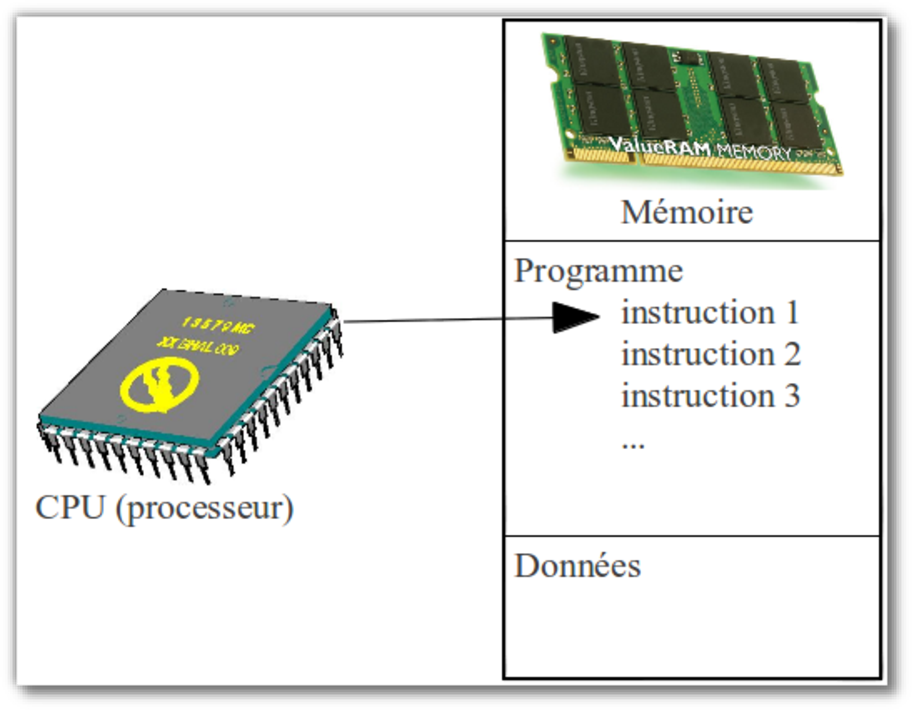
\includegraphics[width=0.45\textwidth]{image/intro-schema-ordi}
			\end{center}
		&
			\textbf{Comment fonctionne le processeur~?}
	
			De façon très simplifiée, on passe par les étapes suivantes~:
	
			\medskip
			\begin{flushleft}
			\begin{enumerate}
			\item Le processeur lit l’instruction courante.
			\item Il exécute cette instruction. Cela peut amener à manipuler les données.
			\item L’instruction suivante devient l’instruction courante.
			\item On revient au point 1.
			\end{enumerate}
			\end{flushleft}
		\\
		\end{tabular}

		On voit qu’il s’agit d’un travail
		automatique ne laissant aucune place à l’initiative~!

\section{Les phases d’élaboration d’un programme}

	Voyons pour résumer un schéma \textbf{simplifié} des phases par
	lesquelles il faut passer quand on développe un programme.

	\begin{tabular}{m{0.25\linewidth}m{0.72\linewidth}}
	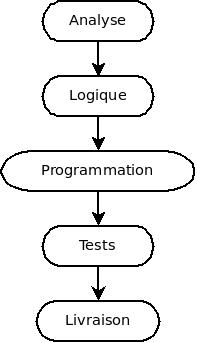
\includegraphics[width=3.5cm]{image/intro-phases-develop}
	&
	\begin{liste}
	\item 
		Lors de \textbf{l’analyse}, le problème doit être
		compris et clairement précisé. Vous aborderez cette phase dans le cours
		d’analyse.
	\item
		Une fois le problème analysé, et avant de passer à la phase de
		programmation, il faut réfléchir à l’\textbf{algorithme} qui va
		permettre de résoudre le problème. C’est à cette phase précise
		que s’attache ce cours.
	\item
		On peut alors \textbf{programmer} cet algorithme dans le langage de
		programmation choisi. Vos cours de langage (Java, Cobol, 
		Assembleur, \dots) sont dédiés à cette phase.
	\item
		Vient ensuite la phase de \textbf{tests} qui ne manquera pas de montrer
		qu’il subsiste des problèmes qu’il
		faut encore corriger. (Vous aurez maintes fois
		l’occasion de vous en rendre compte lors des
		séances de laboratoire)
	\item
		Le produit sans bug (connu) peut être \textbf{mis en application}
		ou \textbf{livré} à la personne qui vous en a passé la commande.
	\end{liste}
	\\
	\end{tabular}
	
	Notons que ce processus n’est pas linéaire. À chaque
	phase, on pourra détecter des erreurs, imprécisions ou oublis des
	phases précédentes et revenir en arrière.

	\textbf{Pourquoi passer par la phase «~logique~» 
		et ne pas directement passer à la programmation~?}
	
	Voilà une question que vous ne manquerez pas de vous poser pendant votre
	apprentissage cette année. Apportons quelques éléments de réflexion.

	\begin{liste}
	\item
		Passer par une phase de «~logique~» permet de séparer deux 
		difficultés~:~quelle est la marche à suivre~? Et comment l’exprimer
		dans le langage de programmation choisi~? Le langage que nous allons
		utiliser en logique est plus souple et plus général que le langage Java
		par exemple (où il faut être précis au «~;~» près).
	\item
		De plus, un algorithme écrit facilite le dialogue dans une équipe de
		développement. «~J’ai écrit un algorithme pour
		résoudre le problème qui nous occupe. Qu’en
		pensez-vous~? Pensez-vous qu’il est correct~?
		Avez-vous une meilleure idée~?~». L’algorithme est plus adapté à la
		communication car plus lisible.
	\item
		Enfin, si la logique est écrite, elle pourra facilement être traduite
		dans n’importe quel langage de programmation. La
		traduction d’un langage de programmation à un autre
		est un peu moins facile à cause des particularités propres à chaque
		langage.
	\end{liste}

	Bien sûr, cela n’a de sens que si le problème présente
	une réelle difficulté logique. Certains problèmes (en pratique,
	certaines parties de problèmes) sont suffisamment simples que pour être
	directement programmés. Mais qu’est-ce
	qu’un problème simple~? Cela va évidemment changer
	tout au long de votre apprentissage. Un problème qui vous paraitra
	difficile en début d’année vous paraitra (enfin, il
	faut l’espérer~!) une évidence en fin
	d’année.

\section{Conclusion}

	L’informatisation de problèmes est un processus essentiellement
	dynamique, contenant des allées-venues constantes entre les différentes
	étapes. Codifier un algorithme dans un langage de programmation
	quelconque n’est certainement pas la phase la plus difficile de ce
	processus. Par contre, élaborer une démarche logique de résolution d’un
	problème est probablement plus complexe.
	
	Le but du cours de \textbf{logique et techniques de programmation} est
	double~:

	\begin{liste}
	\item
		essayer de définir une bonne démarche d’élaboration d’algorithmes
		(apprentissage de la \textbf{logique} de programmation) ;
	\item
		faire comprendre l’intérêt d’utiliser certaines méthodes ou
		\textbf{techniques} classiques qui ont fait leurs preuves.
	\end{liste}

	Le tout devrait avoir pour résultat l’élaboration de \textit{bons
	programmes}, c’est-à-dire \textit{des programmes dont il est facile de
	se persuader qu’ils sont corrects} et des programmes dont la
	maintenance est la plus aisée possible. Dans ce sens, ce cours se situe
	idéalement en aval d’un cours d’\textbf{analyse}, et en amont des cours
	de \textbf{langage de programmation}. Ceux-ci sont idéalement complétés
	par les notions de \textbf{système d’exploitation} et de
	\textbf{fichiers}.

	Afin d’envisager la résolution d’une multiplicité de problèmes prenant
	leur source dans des domaines différents, le contenu minimum de ce
	cours envisage l’étude des points suivants (dans le désordre)~:

	\begin{liste}
	\item 
		la représentation des algorithmes
	\item
		la programmation structurée
	\item
		la programmation procédurale~:~les modules et 
		le passage de paramètres
	\item
		les bases de la programmation orientée objet
	\item
		la logique de traitement des fichiers séquentiels
	\item
		la logique de traitement des tableaux
	\item
		la résolution de problèmes récursifs
	\item
		la logique de traitement des structures de données particulières telles
		que listes, files d’attente, piles, arbres, graphes, tables de hachage,
		etc.
	\end{liste}

	Voilà bien un programme trop vaste pour une année d’étude, même pour un
	cours de 100 heures~! Un choix devra donc être fait et ce, en fonction
	de critères tels que la rapidité d’assimilation, l’intérêt des
	étudiants et les besoins exprimés pour des cours annexes. Les
	matières non traitées en 1\up{ère} année 
	seront étudiées au cours de logique de 2\up{e} année.

\section{Références}
	
	On reprend ici une liste de livres et sites que vous pouvez consulter
	tout au long de votre apprentissage de
	l’algorithmique. Certaines références, plus
	spécifiques, seront fournies avec les chapitres qui les concernent.

	\begin{liste}
	\item 
		Alain Cardon et Christophe Dabancourt~:~«~\textit{Initiation à
		l’algorithmique objet}~» aux éditions Eyrolles. ISBN
		2-212-09258-X
		\textit{Un ouvrage très clair sur l’algorithmique qui
		suit assez bien le cours de logique même si les notations sont un peu
		différentes.}
	\item
		Claude Delannoy~:~«~\textit{Initiation à
		l’informatique}~» aux éditions Eyrolles. 
		ISBN 978-2212088724
		\textit{Un livre pédagogique adapté à un étudiant de première année.}
	\end{liste}

\chapter{Le robot logique \index{Robot logique}}

	\marginicon{objectif}
	Dans ce chapitre nous allons appréhender les bases de la logique de
	programmation au travers d’une petite application
	ludique~:~le «~robot logique~». Nous pourrons ainsi faire connaissance
	avec les concepts suivants~:
	
	\begin{liste}
	\item La séquence
	\item Les choix ou alternatives
	\item Les répétitions
	\item Les modules
	\end{liste}

	Il ne s’agit que d’une introduction ;
	les chapitres suivants nous permettront d’approfondir
	ces concepts.

\section{Le «~robot logique~»}

	Pour introduire les bases de la logique de programmation, nous utilisons
	le «~robot logique~», un programme d’aide à
	l’apprentissage de l’algorithmique conçu par Marc Tommasi
	de l’université de Lille
	3\footnote{\url{http://jrobot.gforge.inria.fr/}}.
	
	\begin{multicols}{2}
	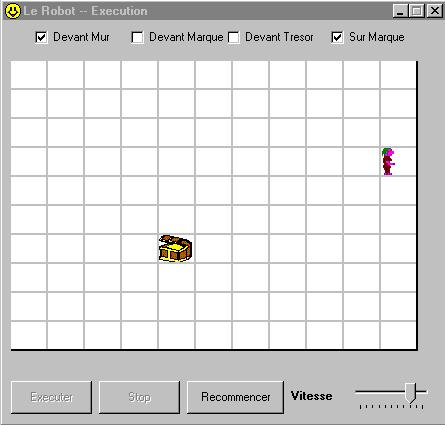
\includegraphics[width=5.553cm,height=5.302cm]{image/robot-grille.pdf}

	Un robot se déplace dans un domaine rectangulaire sous 
	forme d’une grille délimitée par un mur.
	On peut y placer un trésor. Le but est de trouver
	l’algorithme qui va permettre au robot
	d’effectuer une tâche donnée (par exemple trouver le
	trésor). Pour cela, il faut combiner les ordres de base (les
	primitives) qu’il connait (par exemple~:~«~avancer~»,
	«~à droite~», \dots) en utilisant éventuellement des structures
	conditionnelles ou répétitives.

	\end{multicols}
	
	\textbf{Note}~:~Récemment, l’auteur a modifié le graphisme de l’application.
	Le robot apparait comme un pingouin et le trésor est
	devenu un poisson. 
	Le fonctionnement de l’application n’a toutefois pas 
	fondamentalement changé.

	\subsection{Installation}

		Le programme n’est pas installé à l’école.
		Il est possible de l’essayer sans l’installer.
		Pour cela, il faut se rendre sur la page de l’application
		(\url{http://jrobot.gforge.inria.fr/}) et cliquer sur le lien
		\og~Essayez-le~\fg.
		Chez vous, vous pouvez également cliquer sur le lien 
		\og~Téléchargez-le~\fg{} pour l’installer.
		
	\subsection{Utilisation}

		Le robot se configure via deux fenêtres.

		\begin{enumerate}
		\item 
			La première permet de «~programmer~» le robot, 
			lui donner la \textbf{séquence d’instructions}
			qu’il va devoir suivre. 
			Cette fenêtre permet également
			d’indiquer la \textbf{situation initiale}~:~
			position et orientation du robot, position du trésor.
			
		\item 
			La deuxième fenêtre montre la grille avec le robot 
			et permet de voir «~tourner~» le programme.  
		\end{enumerate}

\section{La séquence}

	Nous l’avons vu dans le chapitre
	d’introduction~:~un algorithme est une séquence
	d’instructions élémentaires. Quelles sont les
	instructions élémentaires comprises par le robot~? Les instructions les
	plus rudimentaires sont~:
	
	\begin{Emphase}[definition]{Instructions élémentaires}
		\remonter
		\begin{description}
		\item[Avancer]
			Le robot se déplace d’une case dans la direction vers laquelle il regarde
		\item[Pivoter à droite]
			Le robot tourne d’un quart de tour vers la droite.
			Ainsi, s’il regardait en bas, il regarde à présent à gauche.
		\end{description}
	\end{Emphase}
		
	Nous allons commencer par quelque chose de très simple~:~demandons au
	robot de faire un demi-tour (sur place).

	\begin{Emphase}[exercice]{Exemple~:~demi-tour}

		«~Faire demi-tour~» n’est pas une instruction
		élémentaire comprise par le robot. Il nous faut la découper en une
		séquence d’instructions plus simples. Ici, rien de
		compliqué, il suffit de tourner deux fois d’un quart
		de tour.

		\textbf{Conditions initiales}

		\begin{itemize}
		\item La position et la direction du robot sont aléatoires
		\item La position du trésor n’est pas importante
		\end{itemize}

		\textbf{But}~:~Le robot doit faire demi-tour.

		\textbf{Solution}
		
		\includegraphics{image/robot-demitour}
		
	\end{Emphase}

	Tentons à présent un exercice un peu plus compliqué
	(même si cela n’apparait pas tout de suite)

	
	\begin{Emphase}[exercice]{Exercice~:~avancer de deux cases}

		\textbf{Conditions initiales}

		\begin{itemize}
		\item La position et la direction du robot sont aléatoires
		\item La position du trésor n’est pas importante
		\end{itemize}
		
		\textbf{But}~:~Le robot doit avancer de deux cases dans la direction
		vers laquelle il regarde.

	\end{Emphase}

	Vous avez peut-être trouvé la solution suivante~:
		
	\includegraphics{image/robot-avancer2}
	
	Elle n’est \textbf{pas correcte}~! Pourtant je suis sûr
	que vous l’avez essayé et que le robot a effectivement
	avancé de 2 cases. 
	
	\begin{Emphase}[reflexion]{Test de l’algorithme}

		Si vous avez trouvé la solution ci-dessus, exécutez-la de nombreuses
		fois, vous finirez par tomber sur un cas où cela ne se passe pas bien.
		Pouvez-vous identifier quel est le problème~?

	\end{Emphase}

	Vous l’avez compris, si le robot est à moins de 2 cases
	du mur, il «~fonce~» dans le mur. Il signale ainsi
	qu’il ne peut pas exécuter une instruction du
	programme.
	
	\marginicon{attention}
	Ce n’est pas parce qu’un programme
	fonctionne correctement une fois, qu’il va fonctionner
	toujours. Il peut se produire un bug dans une condition qui
	n’a pas été prévue par le programmeur. Vous en avez
	sûrement tous déjà fait l’expérience avec les
	programmes que vous utilisez.

	Remarquez que le robot ne prend \textbf{jamais
	d’initiative}. Il exécute chaque instruction donnée
	sans se poser de question (est-ce pertinent, nécessaire~?). Il
	n’a d’ailleurs \textbf{aucune idée du
	but à atteindre, du sens de ce qu’il fait}.
	
	Ici, le problème vient également de
	l’énoncé qui ne stipule pas clairement ce
	qu’il faut faire dans ces cas-là.

\section{Poser correctement le problème}

	On a vu que notre robot «~fonce dans le mur~» si on lui demande
	d’avancer alors qu’il fait face à un
	mur. Il ne fait là qu’exécuter scrupuleusement
	l’algorithme qui lui a été fourni. Mais
	qu’aurait-il dû faire~? Nous n’en
	savons rien car l’énoncé ne le dit pas. On pourrait
	envisager que le robot s’arrête, fasse demi-tour,
	tourne en rond, \dots
	
	Cela met en évidence l’importance de la \textbf{phase
	d’analyse} dans le développement d’un
	programme. \textbf{Que faut-il faire exactement~?} Normalement la
	réponse est à chercher chez la personne pour qui on programme\footnote{Et
	à l’école, dans l’énoncé fourni par
	le professeur~!}.
	
	\marginicon{attention}
	Attention~! Ne surtout pas prendre d’initiative
	lorsqu’on programme. Si on ne sait pas quoi faire dans
	un cas précis, il faut repasser par la phase d’analyse
	pour le préciser. Sinon, on obtiendra la plupart du temps un programme
	\textbf{faux, car ne faisant pas ce qui est attendu}.

\section{Les alternatives \index{Alternatives (avec robot)}}

	Reposons le problème précisément~:~on veut que le robot avance de 2
	cases sauf si un mur l’en empêche, auquel cas il
	s’arrête juste devant le mur.
	
	À présent, la séquence d’instructions que le robot doit
	effectuer va dépendre de la situation, de son environnement. Comment
	faire~? Le robot a la possibilité de \textbf{tester son environnement}
	et de réagir en conséquence (en suivant scrupuleusement ce
	qu’on lui a indiqué évidemment). On va pouvoir lui
	donner deux séries d’instructions ; il exécutera la
	première série ou la deuxième en fonction du résultat du test.

	\begin{Emphase}[definition]{Les tests}
	Parmi les tests disponibles on trouve~:
	
		\begin{description}
		\item[devantMur]
			est vrai si le robot fait \textbf{face} à un mur.
		\item[devantTrésor]
			est vrai si le robot fait face au trésor.
		\end{description}
	\end{Emphase}

	De plus, on peut utiliser les opérateurs \textbf{non}, \textbf{et}, 
	\textbf{ou} pour effectuer des \emph{calculs logiques}.
	
	\begin{Emphase}[definition]{Les alternatives}
	\includegraphics[scale=1]{image/robot-si}
	\end{Emphase}

	Lorsque le robot doit exécuter une alternative, il teste la condition
	fournie. Si elle est vraie il exécute la première série
	d’instructions ; sinon, il exécutera la seconde série.
	Ensuite, il passera à la suite de l’algorithme.

	On rencontrera souvent des situations ou la partie «~sinon~» est vide.
	Le robot doit effectuer des actions uniquement si la condition est
	vraie. Si elle est fausse, il ne doit rien faire (il passe à la suite
	du programme)

	\marginicon{attention}
	Une alternative est une instruction qui se place à un endroit précis
	dans la séquence d’instructions. Le robot ne
	l’évalue qu’à ce moment-là et agit en
	conséquence. Il ne s’agit absolument \textbf{pas de
	vérités} qu’on apprend à
	l’ordinateur, qui sont valables à tout moment et
	qu’il doit utiliser à bon escient pour améliorer son
	comportement.

	Ainsi on ne dit pas~:~«~si, à un moment donné, tu es face à un mur,
	n’avance pas si on te le demande~» mais bien quelque
	chose comme~:~«~si tu n’es pas devant un mur
	\textbf{MAINTENANT} alors tu peux avancer~»

	Notez aussi que le robot exécute \textbf{toutes} les instructions liées
	à un test même si cela en modifie le résultat. Ex~:~si on lui demande
	d’avancer deux fois s’il
	n’est pas devant le mur, il le fera même
	s’il se trouve devant le mur après le premier
	avancement.

	Comment utiliser les alternatives pour améliorer notre programme~?
	Commençons par un exemple simple.

	
	\begin{Emphase}[exercice]{Exemple~:~avancer d’une case}

		\textbf{Conditions initiales}

		\begin{itemize}
		\item La position et la direction du robot sont aléatoires
		\item La position du trésor n’est pas importante
		\end{itemize}
		
		\textbf{But}~:~Le robot doit avancer d’\textbf{une
		case} tout droit (dans la direction vers laquelle il regarde). 
		Si un mur l’en empêche, il devra s’arrêter juste devant ce mur.

		\textbf{Solution}~:~
		
		\includegraphics[scale=0.9]{image/robot-avancer1}

	\end{Emphase}
	
	Si cet exemple est bien compris, 
	essayez de résoudre par vous-même celui-ci~:

	
	\begin{Emphase}[exercice]{Exercice~:~avancer de deux cases (amélioré)}

		\textbf{Conditions initiales}

		\begin{itemize}
		\item La position et la direction du robot sont aléatoires
		\item La position du trésor n’est pas importante
		\end{itemize}
		
		\textbf{But}~:~Le robot doit avancer de \textbf{deux cases} tout droit
		(dans la direction vers laquelle il regarde). Si un mur
		l’en empêche, il devra s’arrêter
		juste devant le mur.

	\end{Emphase}

\section{La répétition}

	Continuons notre apprentissage de l’algorithmique et
	posons-nous le problème suivant~:~«~On voudrait que le robot avance
	\textbf{jusqu’au} mur face à lui.~».
	
	Que se passe-t-il ici~? Le robot va devoir avancer un certain nombre de
	fois mais ce nombre est inconnu au moment de
	l’écriture de l’algorithme ; cela va
	dépendre de la situation initiale. Nous allons nous en sortir grâce à
	la structure répétitive. On peut demander à
	l’ordinateur de \textbf{répéter} des instructions. On
	lui fournit également une condition qui lui permet de savoir
	s’il doit continuer ou non cette tâche répétitive.

	
	\begin{Emphase}[definition]{La répétition}
	\includegraphics[scale=1]{image/robot-tq}
	\end{Emphase}

	Lorsqu’il rencontre cette structure, le robot évalue la
	condition. Si elle est vraie, il exécute \textbf{toutes} les
	instructions à l’intérieur du «~\textit{tant que~}»
	puis revient tester la condition. Lorsqu’elle devient
	fausse ou si elle est fausse dès le début, il passe à la suite de
	l’algorithme.
	
	\begin{Emphase}[exercice]{Exercice~:~avancer jusqu’au mur}

		\textbf{Conditions initiales}

		\begin{itemize}
		\item La position et la direction du robot sont aléatoires
		\item La position du trésor n’est pas importante
		\end{itemize}
		
		\textbf{But}~:~Le robot doit avancer jusqu’au mur
		devant lui et s’y arrêter.

	\end{Emphase}

\section{Les marques du robot}

	Imaginons à présent que l’on veuille que le robot
	revienne à sa position de départ après avoir atteint le mur. Le
	problème c’est que le robot n’a pas
	de mémoire. Par contre, il peut laisser une trace de son passage
	(tracer une croix sur la case qu’il occupe).
	
	\marginicon{attention}
	Un ordinateur, lui, possède une mémoire. Il pourrait ainsi retenir les
	coordonnées de la case de départ ou encore le nombre de cases
	parcourues avant d’arriver au mur.

	
	\begin{Emphase}[definition]{Instructions élémentaires}
		\remonter
		\begin{description}
		\item[Marquer]
			Le robot trace une croix sur la case qu’il occupe.
		\item[Effacer marque]
			Le robot efface la croix sur la case qu’il occupe.
		\end{description}
	\end{Emphase}

	\begin{Emphase}{Tests}
		\remonter
		\begin{description}
		\item[devantMarque]
			est vrai si le robot fait face à une marque.
		\item[surMarque]
			est vrai si le robot est sur une marque.
		\end{description}
	\end{Emphase}

	Nous avons à présent tout ce qu’il faut pour résoudre
	notre problème. Il est déjà d’une belle complexité
	mais vous avez tout ce qu’il faut pour le résoudre~:~courage~!

	
	\begin{Emphase}[exercice]{Exercice~:~avancer jusqu’au mur et revenir}

		\textbf{Conditions initiales}

		\begin{itemize}
		\item La position et la direction du robot sont aléatoires
		\item La position du trésor n’est pas importante
		\end{itemize}
		
		\textbf{But}~:~Le robot doit avancer jusqu’au mur
		devant lui, faire demi-tour et revenir à sa position de départ.

	\end{Emphase}

\section{La notion de procédure}

	Pour le problème précédent, vous avez dû, par deux fois, demander au
	robot de faire demi-tour. C’est un problème que vous
	aviez déjà résolu au début de ce chapitre mais vous avez dû, à nouveau,
	expliquer au robot comment faire. C’est gênant~!

	\begin{liste}
	\item 
		L’algorithme devient répétitif car il contient du code dupliqué
		(deux fois «~à droite~»).
	\item 
		À la lecture de l’algorithme, 
		il n’apparait pas clairement qu’on demande au robot 
		d’effectuer un demi-tour
		(en tout cas moins clairement que si on trouvait explicitement
		l’ordre «~demi-tour~»).
	\end{liste}

	\marginicon{reflexion}
	Pourquoi est-ce important que l’algorithme soit lisible
	par un humain puisque c’est le robot
	(l’ordinateur si on généralise) qui va le lire et
	l’exécuter~?

	La solution au problème de duplication de code est fournie par la notion
	de \textit{procédure}.

	\marginicon{definition}
	Une \textbf{procédure} (on dira aussi \textbf{module}, \textbf{fonction}
	ou \textbf{méthode}) est une portion d’algorithme
	auquel on a donné un \textbf{nom} et qui peut être «~utilisé~»
	(\textbf{appelé}) dans d’autres algorithmes.

	Lorsque le robot rencontre un nom de procédure, il exécute toutes les
	instructions de cette procédure puis revient continuer le premier
	algorithme là où il a été interrompu.

	Exemple~:~L’algorithme A appelle la procédure «~Brol~».

	\begin{center}
	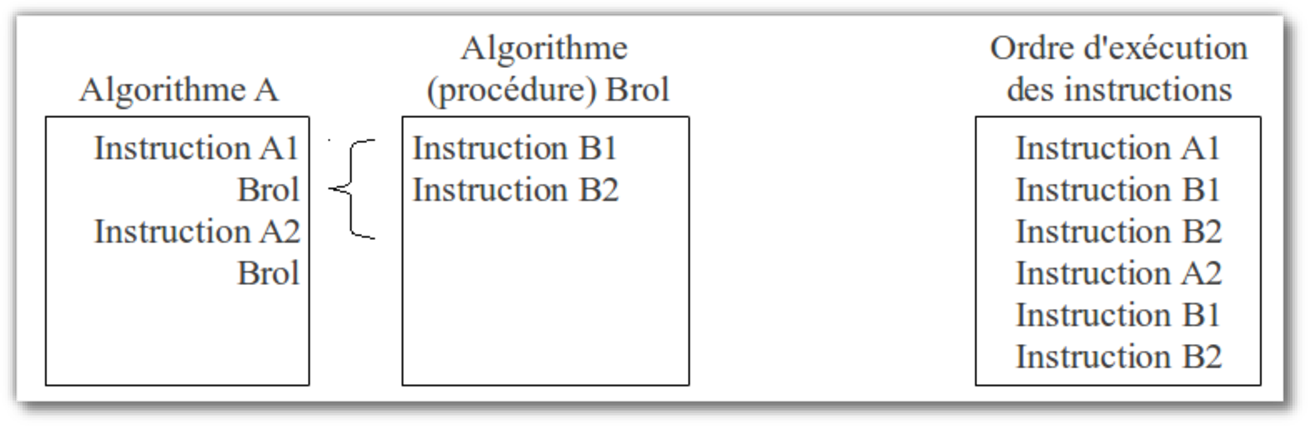
\includegraphics[width=0.9\textwidth]{image/robot-procedure}
	
	{Remarque~:~une procédure est également un algorithme~!}
	\end{center}

	
	\begin{Emphase}[exercice]{Exercice~:~procédure pour le demi-tour}
	
		Écrire une procédure «~demi-tour~» et l’utiliser dans
		le problème précédent (avancer jusqu’au mur et revenir
		au point de départ).
		
		Que pourrions-nous encore écrire comme procédure pour accroitre
		la lisibilité de notre algorithme~?

	\end{Emphase}

\section{Conclusion}

	Le robot nous a permis d’appréhender les principaux
	concepts de l’algorithmique qui vont maintenant nous
	servir pour programmer un ordinateur. 
	
	Une différence importante entre le robot et
	l’ordinateur est que ce dernier possède une
	«~mémoire~» que nous allons pouvoir exploiter au travers du concept de
	variable.

\section{Exercices}

	\subsection{Exercices de réflexion}

		\textit{
		Pour ces exercices, on vous demande de réfléchir sur le concept
		d’algorithme.}

\begin{Exercice}{Un algorithme correct}
Quand peut-on affirmer qu’un algorithme est correct~?
\end{Exercice}

\begin{Exercice}{Unicité d’un algorithme}
	Est-il, selon vous, possible de trouver 
	plusieurs algorithmes différents
	pour résoudre un même problème~?
\end{Exercice}

\begin{Exercice}{Un problème insoluble}
	Pouvez-vous imaginer un problème insoluble pour le robot~?
	C’est-à-dire un problème pour lequel on ne peut pas
	trouver d’algorithme qui le résolve.
\end{Exercice}

	\subsection{Séquences simples}
	
		Pour les exercices suivants, le robot se trouve 
		au départ dans le coin sud-ouest, 
		orienté vers le nord.

\begin{Exercice}{Avancer simplement}
	Le robot doit avancer de trois cases.
\end{Exercice}

\begin{Exercice}{Avancer et tourner}
	Le robot doit avancer de trois cases, tourner à droite, 
	avancer de cinq cases.
\end{Exercice}

\begin{Exercice}{Aller-retour}
	Le robot doit avancer de trois cases, demi-tour, 
	revenir au départ, demi-tour.
\end{Exercice}

\begin{Exercice}{Le carré}
	Le robot se promène sur la grille 
	et décrit un carré de quatre cases sur quatre.
\end{Exercice}
		
	\subsection{Alternatives}

\begin{Exercice}{Avancer d’une case}
	Le robot est placé au hasard.
	Le robot avance si la case devant lui est libre (pas devant un mur).
\end{Exercice}

\begin{Exercice}{Avancer ou demi-tour}
	Le robot est placé au hasard. 
	Le robot avance si la case devant lui est libre,
	sinon il fait demi-tour.
\end{Exercice}

\begin{Exercice}{Chercher le trésor devant}
	Le robot se trouve dans le coin nord-est, orienté vers
	l’ouest ; le trésor est au nord. Le robot doit avancer
	de deux cases au plus. Si le robot se trouve devant le trésor lors de
	son déplacement, il est si content qu’il fait un tour
	sur place avant de se jeter dessus.
\end{Exercice}

\begin{Exercice}{Avancer de deux cases}
	Le robot est placé au hasard. Il avance de 2 cases.
\end{Exercice}


	\subsection{Répétitives}

		\emph{%
		À partir d’ici, les exercices sont difficiles
		(en tout cas en début d’année ; en fin d’année,
		ils devraient vous paraitre plus faciles).
		Si vous n’y arrivez pas tout de suite, c’est normal ; 
		vous pourrez y revenir de temps en temps 
		tout au long de votre apprentissage.
		}

		Le robot se trouve dans le coin sud-ouest, orienté vers le nord.

		\begin{Exercice}{Nord-ouest}
			Le robot doit aller jusqu’au coin nord-ouest.
		\end{Exercice}

		\begin{Exercice}{Nord-ouest et retour}
			Le robot doit aller jusqu’au coin nord-ouest
			puis revenir sur sa case de départ par le même chemin.
		\end{Exercice}

		\begin{Exercice}{Nord-est}
			Le robot doit aller jusqu’au coin nord-est.
		\end{Exercice}

		\begin{Exercice}{Trésor}
			Le robot doit aller jusqu’au trésor qui se trouve
			\begin{itemize}
			\item soit dans le coin nord-est ;
			\item soit dans le coin nord-ouest.
			\end{itemize}
		\end{Exercice}

	\subsection{Modules}

		\begin{Exercice}{Demi-tour}
			Écrire un module qui fait faire un demi-tour au robot.
		\end{Exercice}

		\begin{Exercice}{Tourner}
			Écrire un module qui fait tourner le robot à gauche.
		\end{Exercice}

		\begin{Exercice}{Mur}
			Écrire un module qui déplace le robot
			jusqu’au mur devant lui.
		\end{Exercice}

		\begin{Exercice}{Mur ou trésor}
			Écrire un module qui déplace le robot jusqu’au mur
			devant lui ou le trésor s’il est sur le chemin.
		\end{Exercice}

		\begin{Exercice}{Coin nord-ouest}
			Écrire un module qui déplace le robot vers le coin nord-ouest 
			(orienté vers l’est); on suppose qu’au départ
			le robot est orienté vers l’est.
		\end{Exercice}

		\begin{Exercice}{Un coin}
			Le robot est placé au hasard. 
			Écrire un module qui va dans un coin, peu
			importe lequel. 
		\end{Exercice}

	\subsection{Challenge}

		\begin{Exercice}{Tour du domaine}
			Le robot doit faire le tour du domaine en marquant toutes les cases du
			pourtour, et revenir ensuite à sa position (et son orientation) de
			départ.

			\begin{itemize}
			\item Le robot est situé dans le coin supérieur gauche et regarde à droite.
			\item La position du trésor n’est pas importante.
			\end{itemize}

			\textbf{Conseil}~:~L’utilisation de procédures rendra
			votre programme plus court et plus lisible.
		\end{Exercice}

		\begin{Exercice}{Trouver le trésor (1°)}
			Le robot doit s’arrêter sur le trésor.

			\begin{itemize}
			\item Le robot est situé dans le coin supérieur gauche et regarde à droite.
			\item Le trésor est sur le bord supérieur.
			\end{itemize}

			\textbf{Attention}~:~
			Testez bien votre solution; il existe un cas très particulier.
		\end{Exercice}

		\begin{Exercice}{Trouver le trésor (2°)}
			Le robot doit s’arrêter sur le trésor.

			\begin{itemize}
			\item Le robot est placé aléatoirement et regarde une direction à droite.
			\item Le trésor est placé sur le bord droit.
			\end{itemize}
		\end{Exercice}

		\begin{Exercice}{Trouver le trésor (3°)}
			Le robot doit s’arrêter sur le trésor.

			\begin{itemize}
			\item Le robot est placé aléatoirement et regarde une direction au hasard.
			\item Le trésor est placé sur un bord au hasard.
			\end{itemize}
		\end{Exercice}

		\begin{Exercice}{Marquer le domaine}
			Le robot doit marquer \textbf{complètement} le domaine
			(totalement vide au départ). 
			L’ordre dans lequel il trace les croix n’est pas important.

			\begin{itemize}
			\item
				À vous de choisir la situation initiale du robot qui vous permet de
				résoudre au mieux le problème.
			\end{itemize}
		\end{Exercice}

		\begin{Exercice}{Trouver le trésor (4°)}
			Le robot doit s’arrêter sur le trésor.

			\begin{itemize}
			\item Le robot est situé dans le coin supérieur gauche et regarde à droite.
			\item Le trésor est placé au hasard.
			\end{itemize}
		\end{Exercice}

		\begin{Exercice}{Trouver le trésor (5°)}
			Le robot doit s’arrêter sur le trésor.

			\begin{itemize}
			\item Le robot est placé aléatoirement et regarde une direction au hasard.
			\item Le trésor est placé au hasard.
			\end{itemize}
		\end{Exercice}
			


\chapter{Algorithmes séquentiels}

	\marginicon{objectif}
	Dans ce chapitre, vous apprendrez à écrire un algorithme séquentiel pour
	résoudre un problème informatique. C'est aussi
	l'occasion de fixer la syntaxe du pseudo-code que nous
	allons utiliser. Nous commençons avec les algorithmes
	séquentiels qui sont de simples séquences de suites
	d'instructions. Les structures alternatives et
	répétitives seront vues dans les chapitres suivants.


	\section{Introduction}

		Supposons que nous voulions rédiger une marche
		à suivre détaillée qui explique comment additionner deux fractions. Une
		possibilité de l’écrire en langage «~naturel~» serait la suivante :

		\cadre{
		\begin{pseudo}
			\Stmt - Rechercher le dénominateur commun des deux fractions
			\Stmt - Mettre chaque fraction au même dénominateur
			\Stmt - Additionner les numérateurs des deux fractions,
			\Stmt \Indent ce qui donne le numérateur de la somme
			\Stmt - Simplifier la fraction obtenue
		\end{pseudo}
		}
		
		Cet algorithme, bien que résultant d’un effort
		d’explicitation, est encore très imprécis et risque fort de ne pas
		faciliter l’effort de programmation qui en suivrait. N’oublions pas
		qu’un ordinateur n’est qu’une machine dépourvue de toute intelligence
		et incapable de comprendre les sous-entendus qu’un être humain pourrait
		comprendre !

		De plus, les notions de dénominateur commun et
		de simplification de fraction, qui vous sont 
		familières depuis l'école primaire, 
		ne sont pas immédiates d'un point de
		vue algorithmique. Un algorithme proche d'un langage
		de programmation ne devrait mentionner que les opérations élémentaires
		de calcul telles que $+$, -, $*$, $/$.

		Ceci dit, afin d’être plus proche d’un
		programme écrit dans un langage compréhensible par l’ordinateur,
		l’algorithme ci-dessus pourrait s’écrire :

		\cadre{
		\begin{pseudo}
		\Stmt - Prendre connaissance du premier numérateur et du premier dénominateur ;
		\Stmt - Prendre connaissance du second numérateur et du second dénominateur ;
		\Stmt - Multiplier les deux dénominateurs pour obtenir le dénominateur commun ;
		\Stmt - Multiplier le premier numérateur par le second dénominateur
		\Stmt \Indent et le second numérateur par le premier dénominateur ;
		\Stmt - Additionner ces deux produits pour obtenir le numérateur du résultat ;
		\Stmt - Communiquer ce résultat ainsi que le dénominateur commun.
		\end{pseudo}
		}

		Notons encore que cet algorithme n’est pas le
		plus efficace pour ce type de problème. 
		Il vaudrait mieux utiliser le PPCM 
		(\textit{Plus Petit Commun Multiple}) 
		pour le calcul du dénominateur commun, mais la façon
		de calculer ce dernier serait très fastidieuse à rédiger en langage
		«~naturel~».

		On comprend bien, au travers de cet exemple, que
		le français n’est pas adapté à la description de problèmes au contenu
		mathématique ou scientifique. Le langage naturel est, en effet, un mode
		de représentation trop riche des algorithmes. Il faut comprendre par
		«~riche~», la présence de synonymes, de nombreux mots aux
		significations proches et voisines. L’utiliser amènerait probablement à
		une perte de temps (donc d’argent), et à des risques d’erreurs dans la
		conception des programmes. Il convient dès lors d’élaborer des méthodes
		de représentation plus rigoureuses (donc moins riches) mais nécessitant
		un effort moindre de programmation.

		Ceci dit, le français peut toujours être
		utilisé dans la formalisation d’une première approche de la résolution
		d’un problème devant être traduit ensuite en algorithme puis en
		programme.

	\section{Le pseudo-code}
	
		Les inconvénients de l’utilisation du français dans la représentation
		des algorithmes sont dus à la trop grande richesse de ce langage en
		comparaison à la pauvreté (mais aussi la rigueur) du langage compris
		par la machine. De plus, la lourdeur et la longueur des phrases
		risquent de rendre pénible la relecture et le travail d’élaboration des
		algorithmes. La solution consiste à édulcorer le langage naturel, d’une
		part en remplaçant les noms parfois fastidieux des objets sur lesquels
		portent des opérations par des mots (noms de variables) plus courts,
		d’autre part, en remplaçant les opérations elles-mêmes par des
		opérateurs symboliques suffisamment explicites. De plus, des structures
		types remplaceront les multiples possibilités linguistiques signifiant
		la même chose.

		\marginicon{definition}
		Le \textbf{pseudo-code} ou \textit{Langage de Description des
		Algorithmes} (LDA en abrégé) est un langage formel et symbolique
		utilisant :

		\begin{liste}
		\item
			des \textbf{noms symboliques} destinés à représenter les objets sur
			lesquels s’effectuent des actions ;
		\item
			des \textbf{opérateurs symboliques} ou des mots-clés traduisant les
			opérations primitives exécutables par un exécutant donné ;
		\item
			des \textbf{structures de contrôle} types.
		\end{liste}

		Ce langage repose sur des conventions d’écriture. Il est destiné à
		servir de vecteur de la compréhension permettant par exemple une
		relecture faite par l’élaborateur de l’algorithme lui-même ou faite par
		autrui et facilitant le travail de programmation.

		C’est de cette dernière exigence que nait la polémique consistant à
		savoir jusqu’à quel niveau de détail il convient d’aller dans la
		représentation d’un algorithme ! Nous dirons, pour notre part, qu’il ne
		doit jamais être aussi détaillé que le programme lui-même, celui-ci
		étant, par essence, la description ultime. Point n’est besoin de donner
		deux descriptions quasi identiques d’un algorithme, l’une dans un
		langage \textit{pseudo-codé}, l’autre exprimée dans un langage de
		programmation.

		Nous dirons qu’un algorithme \textit{idéal}, appelé \textbf{algorithme
		général}, exprimé en pseudo-code, devrait se situer à mi-chemin entre
		la démarche globale exprimée dans un langage naturel (langue française)
		ou structuré (ordinogramme) et l’algorithme ultime, c’est-à-dire le
		\textbf{programme}, exprimé en langage de programmation.

		On pourrait d’ailleurs concevoir la possibilité d’établir d’autres
		\textbf{algorithmes plus }\textbf{détaillés} se situant entre
		l’algorithme général et le programme et qui tiendraient compte de
		certaines particularités du langage de programmation dans lequel ils
		sont destinés à être traduits.

		Enfin, et ce n’est pas la chose la moins importante, la définition d’un
		pseudo-code doit être telle qu’il puisse \textbf{faciliter
		l’apprentissage de la logique de programmation} par des personnes
		désireuses de faire de l’informatique un métier. Dans cette optique, il
		est inutile de les embarrasser de contraintes syntaxiques ou autres qui
		risquent de les éloigner du but poursuivi.

		En conclusion, à partir du moment où des conventions sont prises dans un
		contexte bien déterminé (un service informatique d’une entreprise, un
		groupe scolaire,...), il convient que \textbf{tous }respectent ces
		conventions. Ce sera à chacun de juger jusqu’où il ne faut pas aller
		trop loin dans la liberté d’écriture.

	\section{Variables et types}

		Nous savons que les opérations que l’ordinateur devra exécuter portent
		sur des éléments qui sont les \textbf{données} du problème. Lorsqu’on
		attribue un \textbf{nom} et un \textbf{type} à ces données, on parle
		alors de \textbf{variables}. Dans un algorithme, une variable conserve
		toujours son nom et son type, mais peut changer de \textbf{valeur}.
		
		Le \textbf{nom }d’une variable permet de la caractériser et de la
		reconnaitre. Ainsi, dans l’exemple donné ci-dessus, nous pourrions
		donner le nom \textit{num1} au \textit{premier numérateur} et
		\textit{num2} au \textit{second numérateur}, ce qui permet déjà de
		nommer les objets de l’algorithme de façon tout aussi reconnaissable
		mais plus courte et donc plus commode. Quant au \textbf{type} d’une
		variable, il décrit la nature de son contenu.

		\subsection{Les types autorisés}

			Dans un premier temps, les seuls \textbf{types} utilisés sont les
			suivants :
			
			\begin{center}
			\tablehead{}
			\begin{tabular}[t]{p{2cm}|p{12cm}}
			\raggedleft  \textstyleMotCl{entier} &
			 pour les nombres entiers\\
			\raggedleft  \textstyleMotCl{réel} &
			 pour les nombres réels\\
			\raggedleft  \textstyleMotCl{caractère} &
			 pour les différentes lettres et caractères (par
			exemple ceux qui apparaissent sur un clavier : ‘a’, ‘1’, ‘\#’, etc…)\\
			\raggedleft  \textstyleMotCl{chaine} &
			{ pour les variables contenant plusieurs
			caractères ou aucun (la chaine vide)}
			(par exemple : "Bonjour", "Bonjour le monde", "a", "", etc.)
			\\
			\raggedleft  \textstyleMotCl{booléen} &
			 les variables de ce type ne peuvent valoir que
			\textbf{vrai} ou \textbf{faux}\\
			\end{tabular}
			\end{center}
			
			On veillera au cours de logique à ne pas utiliser les valeurs 0 et 1
			pour les variables booléennes, même si leur emploi est correct dans
			beaucoup de langages de programmation.

			
			\begin{Emphase}[exercice]{Exercices}
				Quel(s) type(s) de données utiliseriez-vous 
				pour représenter 
				\begin{itemize}
					\item une date du calendrier ?
					\item un moment dans la journée ?
					\item le prix d'un produit en grande surface ?
					\item votre nom ?
					\item vos initiales ?
					\item votre adresse ?
				\end{itemize}
				
				\bigskip
				
			\end{Emphase}

		\subsection{Déclaration de variables}

			La déclaration d’une variable est l’instruction 
			qui définit son nom et son type. On pourrait écrire :

			\cadre{
			\begin{pseudo}
			\Stmt num1 et num2 seront les noms de deux objets destinés à recevoir
			\Stmt les numérateurs des fractions, c’est-à-dire des nombres à valeurs entières.
			\end{pseudo}
			}
			
			Mais, bien entendu, cette formulation, trop proche du
			langage parlé, serait trop floue et trop longue. 
			Dès lors, nous abrégerons par :

			\cadre{
			\begin{pseudo}
			\Declare{num1, num2}{entiers}
			\end{pseudo}
			}

			\marginicon{definition}
			L’ensemble des instructions de la forme

			\cadre{
			\begin{pseudo}
			\Declare{variable1, variable2,\ldots}{type}
			\end{pseudo}
			}

			forme la partie d’un algorithme nommée 
			\textbf{déclaration des variables}. 
			La déclaration des informations apparaitra toujours en
			début d’algorithme, ou dans un bloc annexe appelé 
			\textbf{dictionnaire des variables} 
			ou encore \textbf{dictionnaire des données}.

			Par exemple, pour l’algorithme des fractions, la déclaration des
			informations pourrait être la suivante :

			\cadre{
			\begin{pseudo}
			\Declare{num1, den1, num2, den2, numRes, denRes}{entiers}
			\end{pseudo}
			}

			avec la signification suivante :

			\begin{liste}
			\item
				\textstyleCodeInsr{num1 (num2)}~: le numérateur 
				de la première (seconde) fraction ;
			\item
				\textstyleCodeInsr{den1 (den2)}~: le dénominateur 
				de la première (seconde) fraction ;
			\item
				\textstyleCodeInsr{numRes (denRes)}~:
				le numérateur (dénominateur) du résultat.
			\end{liste}
			
			\marginicon{attention}
			Attention, lors de la déclaration d’une variable, celle-ci n’a pas de
			valeur ! Nous verrons plus loin que c’est l’instruction
			d’\textbf{affectation} qui va servir à donner un contenu aux variables
			déclarées. En logique, nous n’envisageons pas d’\textit{affectation par
			défaut} consistant à donner une valeur initiale de façon automatique
			aux variables déclarées (par exemple 0 pour les variables numériques,
			comme c’est le cas dans certains langages informatiques).

		\subsection{Comment nommer correctement une variable ?}

			Le but est de trouver un nom qui soit suffisamment court tout en restant
			explicite (ainsi \textstyleCodeInsr{num1} est plus approprié pour
			désigner le \textit{premier numérateur }que \textstyleCodeInsr{zozo1},
			\textstyleCodeInsr{tintin}, \textstyleCodeInsr{bidule,
			premierNumérateur}) et qui ne prête pas à confusion (par exemple
			appeler \textbf{den} la variable représentant le numérateur.
			Il faut aussi tenir compte que les
			langages de programmation imposent certaines limitations (parfois
			différentes d'un langage à l'autre)
			ce qui peut nécessiter une modification du nom lors de la traduction.

			Voici quelques règles et limitations traditionnelles dans les langages
			de programmation:

			\begin{liste}
			\item 
				Un nom de variable est généralement une suite de caractères
				alphanumériques d’un seul tenant (pas de caractères blancs) et ne
				commençant jamais par un chiffre. Ainsi \textstyleCodeInsr{x1} est
				correct mais non \textstyleCodeInsr{1x}. 
			\item 
				Pour donner un nom composé à une variable, on peut utiliser le «~tiret
				bas~» ou \textit{underscore} (par ex. premier\_numérateur) mais on
				déconseille d’utiliser le signe «~–~» qui est plutôt réservé à la
				soustraction. Ainsi, dans la plupart des langages,
				\textstyleCodeInsr{premier-numérateur} serait interprété comme la
				soustraction des variables \textstyleCodeInsr{premier} et
				\textstyleCodeInsr{numérateur}. (Signalons que le tiret 
				\textcolor{black}{«~–~»} est autorisé en Cobol, où il récupère son rôle
				arithmétique s’il est précédé et suivi d’au moins un blanc).
			\item 
				Une alternative à l’utilisation du tiret bas pour l’écriture de noms de
				variables composés est la notation «~chameau~» (\textit{camelCase} en
				anglais), qui consiste à mettre une majuscule au début des mots
				(généralement à partir du deuxième), par exemple
				\textstyleCodeInsr{premierNombre} ou
				\textstyleCodeInsr{dateNaissance}.
			\item
				Les indices et exposants sont proscrits (par ex.
				\textstyleCodeInsr{x}\textstyleCodeInsr{\textsubscript{1}},
				\textstyleCodeInsr{z}\textstyleCodeInsr{\textsubscript{6}} ou
				\textstyleCodeInsr{m²)}
			\item
				Les mots clés du langage sont interdits (par exemple
				\textstyleMotCl{for}, \textstyleMotCl{if}, 
				\textstyleMotCl{while }pour Java et Cobol) et on déconseille 
				d'utiliser les mots-clés du pseudo-code (tels que
				\textstyleMotCl{\textsf{lire}}, 
				\textstyleMotCl{\textsf{afficher}}, 
				\textstyleMotCl{\textsf{pour}}…)
			\item
				Certains langages n’autorisent pas les caractères accentués (tels que
				\textit{à, ç, ê, ø,} etc.) ou les lettres des alphabets non latins
				(tel que ${\Delta}$) mais d’autres oui ; certains font la distinction
				entre les minuscules et majuscules, d’autres non. En logique, nous
				admettons dans noms de variables les caractères accentués du français,
				par ex. : durée, intérêts, etc.
			\end{liste}

			Il est impossible de décrire ici toutes les particularités des
			différents langages, le programmeur se reportera aux règles spécifiques
			du langage qu’il sera amené à utiliser.

			
			\begin{Emphase}[exercice]{Exercice : Déclarer une date}
				Déclarer le(s) variable(s) permettant de représenter la date
				d'anniversaire de quelqu'un.
			\end{Emphase}
			
			
			\begin{Emphase}[exercice]{Exercice : Déclarer un rendez-vous}
				Déclarer le(s) variable(s) permettant de représenter
				l'heure de début, l'heure de fin et
				l'objet d 'un rendez-vous.
			\end{Emphase}

	\section{Opérateurs et expressions}
	
		Les opérateurs agissent sur les variables et les constantes pour former
		des \textbf{expressions}. Une expression est donc une combinaison
		\textbf{cohérente} de variables, de constantes et d’opérateurs,
		éventuellement accompagnés de parenthèses.
	
		\subsection{Opérateurs arithmétiques élémentaires}
	
			Ce sont les opérateurs binaires bien connus :
	
			\begin{center}
			\tablehead{}
			\begin{supertabular}{m{1cm}|m{12cm}}
			\raggedleft  \textstyleCodeInsr{+} & addition\\
			\raggedleft  \textstyleCodeInsr{-} & soustraction\\
			\raggedleft  \textstyleCodeInsr{*} & multiplication\\
			\raggedleft  \textstyleCodeInsr{/} & division réelle\\
			\end{supertabular}
			\end{center}
	
			Ils agissent sur des variables ou expressions à valeurs entières ou
			réelles. Plusieurs opérateurs peuvent être utilisés pour former des
			expressions plus ou moins complexes, en tenant compte des règles de
			calcul habituelles, notamment la priorité de la multiplication et de la
			division sur l’addition et la soustraction. Il est aussi permis
			d’utiliser des parenthèses, par exemple \textstyleCodeInsr{a – (b + c *
			d)/x}. Tout emploi de la division devra être accompagné d’une réflexion
			sur la valeur du dénominateur, une division par 0 entrainant toujours
			l’arrêt d’un algorithme.
	
		\subsection{DIV et MOD}
	
			Ce sont deux opérateurs très importants qui ne peuvent s’utiliser
			qu’avec des variables entières :
	
			\begin{center}
			\tablehead{}
			\begin{supertabular}{m{1cm}|m{12cm}}
			\raggedleft  \textstyleCodeInsr{DIV} & division entière\\
			\raggedleft  \textstyleCodeInsr{MOD} & reste de la division entière\\
			\end{supertabular}
			\end{center}
	
			Par exemple, \textstyleCodeInsr{47 DIV 7} donne 6 tandis que
			\textstyleCodeInsr{47 MOD 7} donne \textstyleCodeInsr{5}.
	
		\subsection{Fonctions mathématiques complexes}
	
			L’élévation à la puissance sera notée \textstyleCodeInsr{**} ou
			\textstyleCodeInsr{\^{}} . Pour la racine carrée d’une variable x nous
			écrirons  $\sqrt{x}$ \textit{.} Attention, pour ce dernier, de veiller
			à ne l’utiliser qu’avec un radicant positif !
	
			\textbf{Exemple} : 
			$(-b+\sqrt{(b\ast \ast 2-4\ast a\ast c)})/(2\ast a)$
			
			Mais on peut aussi accepter la notation mathématique usuelle
			$\frac{-b+\sqrt{b^{2}-4\ast a\ast c}}{2\ast a}$ 
	
			\marginicon{reflexion}
			Pourquoi ne pas avoir écrit «~\textstyleCodeInsr{4ac}~» et
			«~\textstyleCodeInsr{2a}~» ?
	
			Si nécessaire, on se permettra d'utiliser les autres
			fonctions mathématiques sous leur forme la plus courante dans la
			plupart des langages de programmation (exemples :
			$sin(x)$, $tan(x)$, $log(x)$, $exp(x)$, ...)
			
		
		\subsection{Opérateurs de comparaison}
	
			Ces opérateurs agissent généralement sur des variables numériques ou des
			chaines et donnent un résultat booléen.
	
			\begin{center}
			\tablehead{}
			\begin{supertabular}{m{2cm}|m{11cm}}
			\raggedleft  \textstyleCodeInsr{=} & égal\\
			\raggedleft  \textstyleCodeInsr{{\textless}{\textgreater}}
				ou \textstyleCodeInsr{${\neq}$} &  différent de\\
			\raggedleft  \textstyleCodeInsr{\textless} & (strictement) plus petit que\\
			\raggedleft  \textstyleCodeInsr{\textgreater} & (strictement) plus grand que\\
			\raggedleft  \textstyleCodeInsr{${\leq}$} & plus petit ou égal\\
			\raggedleft  \textstyleCodeInsr{${\geq}$} & plus grand ou égal\\
			\end{supertabular}
			\end{center}
	
			Pour les chaines, c'est l’ordre alphabétique qui
			détermine le résultat (par exemple
			\textstyleCodeInsr{{\textquotedbl}milou{\textquotedbl} {\textless}
			{\textquotedbl}tintin{\textquotedbl}} est \textbf{vrai} de même que
			\textstyleCodeInsr{{\textquotedbl}assembleur{\textquotedbl}
			}\textstyleCodeInsr{${\leq}$}\textstyleCodeInsr{
			{\textquotedbl}java{\textquotedbl}})
			
	
		\subsection{Opérateurs logiques}
	
			Ils agissent sur des expressions booléennes (variables ou expressions à
			valeurs booléennes) pour donner un résultat du même type.
	
			\begin{center}
			\tablehead{}
			\begin{supertabular}{m{1cm}|m{12cm}}
			\raggedleft  \textstyleCodeInsr{NON} & négation\\
			\raggedleft  \textstyleCodeInsr{ET} & conjonction logique\\
			\raggedleft  \textstyleCodeInsr{OU} & disjonction logique\\
			\end{supertabular}
			\end{center}
	
			Pour rappel, \textstyleCodeInsr{cond1 ET cond2} n’est vrai que lorsque
			les deux conditions sont vraies. \textstyleCodeInsr{cond1 OU cond2} est
			toujours vrai, sauf quand les deux conditions sont fausses.
	
			Veillez à mettre des parenthèses dans le cas de combinaisons de ET et de
			OU : \textstyleCodeInsr{(cond1 ET cond2) OU cond3} étant différent de
			\textstyleCodeInsr{cond1 ET (cond2 OU cond3).} En cas
			d'oubli de parenthèses, il faudra se rappeler que
			\textstyleCodeInsr{ET} est prioritaire sur le \textstyleCodeInsr{OU}.
			
			Pour rappel aussi, pour un booléen \textstyleCodeInsr{ok}~: 
			\textstyleCodeInsr{ok = faux} est équivalent à \textstyleCodeInsr{NON ok},
			\textstyleCodeInsr{ok = vrai} est équivalent à \textstyleCodeInsr{ok} et 
			\textstyleCodeInsr{NON NON ok} est équivalent à \textstyleCodeInsr{ok}.
			Dans les trois cas, nous préconiserons la seconde écriture.
	
		\subsection{Évaluation complète et court-circuitée}
	
			On définit deux modes d’évaluation des opérateurs \textstyleCodeInsr{ET}
			et \textstyleCodeInsr{OU} :
	
			\begin{description}
			\item[l’évaluation \textit{complète}]
				pour connaitre la valeur de
				\textstyleCodeInsr{cond1 ET cond2} (respectivement
				\textstyleCodeInsr{cond1 OU cond2}), les deux conditions sont chacune
				évaluées, après quoi on évalue la valeur de vérité de l’ensemble de
				l'expression.
			\item[l’évaluation \textit{court-circuitée}]
				dans un premier temps, seule la
				première condition est testée. Dans le cas du \textstyleCodeInsr{ET},
				si \textstyleCodeInsr{cond1} s’avère faux, il est inutile d’évaluer
				\textstyleCodeInsr{cond2} puisque le résultat sera faux de toute façon
				; l’évaluation de \textstyleCodeInsr{cond2} et de l’ensemble de la
				conjonction ne se fera que si \textstyleCodeInsr{cond1} est vrai. De
				même, dans le cas du \textstyleCodeInsr{OU}, si
				\textstyleCodeInsr{cond1} s’avère vrai, il est inutile d’évaluer
				\textstyleCodeInsr{cond2} puisque le résultat sera vrai de toute façon
				; l’évaluation de \textstyleCodeInsr{cond2} et de l’ensemble de la
				disjonction ne se fera que si \textstyleCodeInsr{cond1} est faux.
			\end{description}
	
			Dans le cadre de ce cours, nous opterons pour la deuxième 
			interprétation.
			Montrons son avantage sur un exemple.
			Considérons	l’expression 
			\textstyleCodeInsr{n }\textstyleCodeInsr{${\neq}$}\textstyleCodeInsr{ 0
			ET m/n {\textgreater} 10}. Si on teste sa valeur de vérité avec une
			valeur de \textstyleCodeInsr{n} non nulle, la première condition est
			vraie et le résultat de la conjonction dépendra de la valeur de la
			deuxième condition. Supposons à présent que \textstyleCodeInsr{n} soit
			nul. L’évaluation court-circuitée donne le résultat \textbf{faux}
			immédiatement après test de la première condition sans évaluer la
			seconde, tandis que l’évaluation complète entrainerait un arrêt de
			l’algorithme pour cause de division par 0 !
	
			Noter que l’évaluation court-circuitée a pour conséquence la
			non-commutativité du \textstyleCodeInsr{ET} et du
			\textstyleCodeInsr{OU~}: \textstyleCodeInsr{cond1 ET cond2} n’est donc
			pas équivalent à \textstyleCodeInsr{cond2 ET cond1}, puisque l’ordre
			des évaluations des deux conditions entre en jeu.~Nous conseillons
			cependant de limiter les cas d’utilisation de l’évaluation
			court-circuitée et d'opter pour des expressions dont
			l’évaluation serait similaire dans les deux cas. La justification
			d’utiliser l’évaluation court-circuitée apparaitra dans plusieurs
			exemples tout au long du cours.
	
		\subsection{Manipuler les chaines}
		
			Pour les chaines, nous allons introduire quelques notations\footnote{
			Le lecteur averti reconnaitra la notation modulaire}
			qui vont nous permettre de les manipuler plus facilement.
		
			\begin{liste}
			\item \textstyleCodeInsr{long(maChaine)}
				donne la taille (le nombre de caractères) de la chaine 
				\textstyleCodeInsr{maChaine}.
			\item \textstyleCodeInsr{car(maChaine,pos)}
				donne le caractère en position \textstyleCodeInsr{pos} 
				(à partir de 1) dans la chaine \textstyleCodeInsr{maChaine}.
			\item \textstyleCodeInsr{concat(maChaine1,maChaine2)}
				concatène les chaines \textstyleCodeInsr{maChaine1} 
				et \textstyleCodeInsr{maChaine2}.
				(ex: \textstyleCodeInsr{concat("Bon","jour")} donne \textstyleCodeInsr{"Bonjour"})
			\end{liste}

		\subsection{Manipuler les caractères}

			Introduisons également quelques notations pour les caractères.

			\begin{liste}
			\item \textstyleCodeInsr{chaine(car)} transforme le caractère \textstyleCodeInsr{car} en une chaine de taille 1.
			\item \textstyleCodeInsr{estLettre(car)} est vrai si le caractère \textstyleCodeInsr{car} est une lettre
				(idem pour \textstyleCodeInsr{estChiffre}, 
				\textstyleCodeInsr{estMajuscule}, 
				\textstyleCodeInsr{estMinuscule}).
			\item \textstyleCodeInsr{majuscule(car)} donne la majuscule de la lettre \textstyleCodeInsr{car}
				(idem pour \textstyleCodeInsr{minuscule}).
			\item \textstyleCodeInsr{position(car)} donne la position de \textstyleCodeInsr{car} dans l'alphabet (ex: \textstyleCodeInsr{numLettre('E')} donne 5, 
			idem pour \textstyleCodeInsr{numLettre('e')}).
			\item \textstyleCodeInsr{lettre(num)} l'inverse de la précédente (ex: \textstyleCodeInsr{lettre(4)} donne le caractère 'D').
			\end{liste}

			 
	\section{L’affectation d’une valeur à une variable}

		Cette opération est probablement l’opération la plus importante. En
		effet, une variable ne prend son sens réel que si elle reçoit à un
		moment donné une valeur. Il y a deux moyens de donner une valeur à une
		variable.

		\subsection{Affectation externe }

			On parle d’\textbf{affectation externe} lorsque la valeur à affecter à
			une variable est donnée par l’utilisateur qui la communique à
			l’exécutant quand celui-ci le lui demande : cette valeur est donc
			\textit{externe} à la procédure \ (l’ordinateur ne peut la deviner
			lui-même !)

			L’affectation externe est donc la primitive qui permet de recevoir de
			l’utilisateur, au moment où l'algorithme se déroule,
			une ou plusieurs valeur(s) et de les affecter à des variables en
			mémoire. Nous noterons :

			\cadre{
			\begin{pseudo}
			\Read liste\_de\_variables\_à\_lire
			\end{pseudo}
			}
			
			{\bfseries Exemples}
			
			\cadre{
			\begin{pseudo}
			\Read nombre1, nombre2
			\Read num1, den1, num2, den2
			\end{pseudo}
			}
			
			L’exécution de cette instruction provoque une
			pause dans le déroulement de l’algorithme : l’exécutant demande alors à
			l’utilisateur les valeurs des variables à lire. Ces valeurs viennent
			donc de l’\textit{extérieur~}; une fois introduites dans le système,
			elles sont affectées aux variables concernées et l’algorithme peut
			reprendre son cours. 
			Les possibilités d'introduction de données 
			sont nombreuses : citons par exemple l’encodage de
			données au clavier, un clic de souris, le toucher d'un
			écran tactile, des données provenant d’un fichier, etc.

		\subsection{Affectation interne }

			On parle d’affectation interne lorsque la valeur d’une variable est
			«~calculée~» par l’exécutant de l’algorithme lui-même à partir de
			données qu’il connait déjà :

			\cadre{
			\begin{pseudo}
			\Let nomVariable \Gets expression
			\end{pseudo}
			}
			
			Rappelons qu’une \textbf{expression} 
			est une combinaison de variables et
			d’opérateurs. L'expression a une valeur.
			
			\subsubsection*{Exemples d'affectation corrects}
			
			\cadre{
			\begin{pseudo}
			\Let somme \Gets nombre1 + nombre2
			\Let denRes \Gets den1 * den2
			\Let cpt \Gets cpt + 1
			\Let delta \Gets b**2 – 4*a*c
			\Let test \Gets a < b \RComment pour une variable logique
			\Let maChaine \Gets "Bon"
			\Let uneChaine \Gets concat(maChaine, "jour")
			\end{pseudo}
			}
			
			\subsubsection*{Exemples d'affectation incorrects}
			
			\cadre{
			\begin{pseudo}
			\Let somme + 1 \Gets 3
			\RComment somme + 1 n'est pas une variable
			\Let somme \Gets 3n
			\RComment 3n n'est ni un nom de variable correct ni une expression correcte
			\end{pseudo}
			}
			
			\subsubsection*{Remarques}

			\begin{liste}
			\item
				Il est de règle que le résultat de l’expression à droite du signe
				d’affectation ($\gets$) soit de
				même type que la variable à sa gauche. On tolère certaines exceptions
				:
				\begin{liste}
				\item
					\textstyleCodeInsr{varEntière}{ $\gets$ }\textstyleCodeInsr{varRéelle} : 
					dans ce cas le contenu de la variable sera la valeur \textbf{tronquée}
					de l’expression réelle. 
					Par exemple si «~\textstyleCodeInsr{nb}~» est
					une variable de type entier, son contenu après l’instruction
					«~\textstyleCodeInsr{nb}{ $\gets$ }\textstyleCodeInsr{$15/4$}~» 
					sera 3
				\item 
					\textstyleCodeInsr{varRéelle}{ $\gets$ }\textstyleCodeInsr{varEntière} :
					ici, il n'y a pas de perte de valeur.
				\item 
					\textstyleCodeInsr{varChaine}{ $\gets$ }\textstyleCodeInsr{varCaractère} : 
					équivalent à \textstyleCodeInsr{varChaine}{ $\gets$ }\textstyleCodeInsr{chaine(varCaractère)}.
					
					Le contraire n'est évidemment pas accepté.
				\end{liste}
			\item 
				Seules les variables déclarées peuvent être affectées, que ce soit par
				l’affectation externe ou interne!
			\item 
				Nous ne mélangerons pas la déclaration d’une variable et son
				affectation interne dans une même ligne de code, donc pas
				d’instructions hybrides du genre 
				\textsf{x}{ $\gets$ }\textstyleCodeInsr{2 : entier} ou encore 
				\textsf{x~: entier(0)}.
			\item 
				Pour l’affectation interne, toutes les variables apparaissant dans
				l'\textstyleCodeInsr{expression} doivent avoir été affectées
				préalablement. Le contraire provoquerait un arrêt de l’algorithme.
			\end{liste}
			
	\section{Communication des résultats}

		L’instruction de communication des résultats consiste à donner à
		l’extérieur (donc à l’utilisateur) la valeur d’un résultat 
		calculé au cours de l’exécution de l’algorithme. Nous écrirons :

			\cadre{
			\begin{pseudo}
			\Write \textit{expression} ou \textit{liste de variables séparées par des virgules}
			\end{pseudo}
			}

		qui signifie que la valeur d’une expression (ou celles des différentes
		variables mentionnées) sera fournie à l’utilisateur (par exemple par un
		affichage à l’écran ou par impression sur listing via l’imprimante,
		etc\dots).

		\subsubsection*{Remarques}

		\begin{liste}
		\item
			Ce ne serait pas une erreur fondamentale de remplacer
			\textstyleCodeInsr{lire} par \textstyleCodeInsr{recevoir} ou
			\textstyleCodeInsr{afficher} par \textstyleCodeInsr{écrire}. Il n’y a
			évidemment pas de confusion possible à partir du moment où l’on sait
			qu’il s’agit de primitives d’échange entre l’extérieur et l’ordinateur
			exécutant la procédure, mais par principe, il est conseillé d’utiliser
			une syntaxe commune et limitée à un petit nombre de mots clés.
		\item
			Comme pour l’affectation interne, on ne peut \textstyleCodeInsr{afficher}
			que des expressions dont les variables qui la composent ont été 
			affectées préalablement.
		\end{liste}

	\section{Structure générale d’un algorithme}

		La traduction d’un algorithme en pseudo-code constituera le contenu d’un
		\textstyleMotCl{module}. Un module contient donc la solution
		algorithmique d’un problème donné (ou d’une de ses parties). Sa
		structure générale sera la suivante :

		\cadre{
		\begin{pseudo}
		\Module{nomDuModule}{}{}
			\Stmt \textit{déclaration des variables et constantes utilisées dans le module}
			\Stmt \textit{lecture des données}
			\Stmt \textit{instructions utilisant les données lues}
			\Stmt \textit{communication des résultats}
		\EndModule
		\end{pseudo}
		}		

		\subsubsection*{Remarques}
		
		\begin{liste}
		\item {
			Le code d'un algorithme sera toujours compris entre la
			première ligne, appelée «~entête~» qui commence par 
			le mot «~module~»
			suivi du nom choisi pour l'algorithme, et la ligne
			finale «~fin module~». Le code compris entre l'entête
			et la ligne finale sera toujours légèrement décalé vers la droite,
			c'est un premier exemple
			d'\textbf{indentation} indispensable pour la
			lisibilité d'un programme, nous y reviendrons lors de
			l'étude des structures alternatives et répétitives.}
		\item {
			Comme pour les variables, le nomDuModule devra être approprié au contenu
			! Par exemple, \textstyleCodeInsr{sommerNombres)}, 
			\textstyleCodeInsr{additionnerFractions()} plutôt que 
			\textstyleCodeInsr{goPartez()}!
			Le rôle des parenthèses qui suivent le nom du module sera expliqué plus
			tard.}
		\item {
			Il va de soi que toutes les parties de cette structure générale ne
			seront pas toujours nécessaires : certains algorithmes ne nécessiteront
			pas de lecture de données, d'autres ne devront pas
			communiquer des résultats,...}
		\item {
			Pour la lisibilité, on veillera toujours à ce qu'un module
			tienne sur une vingtaine de lignes (donc, en pratique, sur un écran 
			de 40 x 80 caractères ou une page). Ceci implique que si le module 
			devait être plus long, il faudrait le découper, comme nous le verrons 
			plus loin.}
		\end{liste}

		\bigskip

		Analysons les algorithmes suivants~:
		
		\cadre{
		\begin{pseudo}
		\Module{exempleValide}{}{}
			\Declare{a, b, c}{entiers}
			\Let a \Gets 12
			\Let b \Gets 5
			\Let c \Gets a - b
			\Let a \Gets a + c
			\Let b \Gets a
		\EndModule
		\end{pseudo}
		}
		
		\begin{center}
		\tablehead{}
		\begin{supertabular}
			{m{3cm}m{3cm}m{3cm}m{3cm}}
			\multicolumn{1}{|m{3cm}|}{} &
			\multicolumn{1}{m{3cm}|}{a} &
			\multicolumn{1}{m{3cm}|}{b} &
			\multicolumn{1}{m{3cm}|}{c}\\\hline
			
			\multicolumn{1}{|m{3cm}|}{\textstyleCodeInsr{a, b, c : entiers}} &
			\multicolumn{1}{m{3cm}|}{indéfini} &
			\multicolumn{1}{m{3cm}|}{indéfini} &
			\multicolumn{1}{m{3cm}|}{indéfini}\\\hline
			
			\multicolumn{1}{|m{3cm}|}{\textstyleCodeInsr{a}{ $\gets$ } 12} &
			\multicolumn{1}{m{3cm}|}{12} &
			\multicolumn{1}{m{3cm}|}{indéfini} &
			\multicolumn{1}{m{3cm}|}{indéfini}\\\hline
			
			\multicolumn{1}{|m{3cm}|}{\textstyleCodeInsr{b}{ $\gets$ } 5} &
			\multicolumn{1}{m{3cm}|}{12} &
			\multicolumn{1}{m{3cm}|}{5} &
			\multicolumn{1}{m{3cm}|}{indéfini}\\\hline
			
			\multicolumn{1}{|m{3cm}|}{\textstyleCodeInsr{c}{ $\gets$ }  \textstyleCodeInsr{a - b}} &
			\multicolumn{1}{m{3cm}|}{12} &
			\multicolumn{1}{m{3cm}|}{5} &
			\multicolumn{1}{m{3cm}|}{7}\\\hline
			
			\multicolumn{1}{|m{3cm}|}{\textstyleCodeInsr{a}{ $\gets$ }  \textstyleCodeInsr{a + c}} &
			\multicolumn{1}{m{3cm}|}{19} &
			\multicolumn{1}{m{3cm}|}{5} &
			\multicolumn{1}{m{3cm}|}{7}\\\hline
			
			\multicolumn{1}{|m{3cm}|}{\textstyleCodeInsr{b}{ $\gets$ }  \textstyleCodeInsr{a}} &
			\multicolumn{1}{m{3cm}|}{19} &
			\multicolumn{1}{m{3cm}|}{19} &
			\multicolumn{1}{m{3cm}|}{7}\\\hline
			
		\end{supertabular}
		\end{center}

		\bigskip
		
		\bigskip

		\cadre{
		\begin{pseudo}
		\Module{exempleInvalide}{}{}
			\Declare{a, b, c}{entiers}
			\Let a \Gets 12
			\Let c \Gets a - b
			\Let d \Gets c - 2
		\EndModule
		\end{pseudo}
		}
		
		\begin{center}
		\tablehead{}
		\begin{supertabular}
			{m{3cm}m{3cm}m{3cm}m{3cm}}
			\multicolumn{1}{|m{3cm}|}{} &
			\multicolumn{1}{m{3cm}|}{a} &
			\multicolumn{1}{m{3cm}|}{b} &
			\multicolumn{1}{m{3cm}|}{c}\\\hline
			
			\multicolumn{1}{|m{3cm}|}{\textstyleCodeInsr{a, b, c : entiers}} &
			\multicolumn{1}{m{3cm}|}{indéfini} &
			\multicolumn{1}{m{3cm}|}{indéfini} &
			\multicolumn{1}{m{3cm}|}{indéfini}\\\hline
			
			\multicolumn{1}{|m{3cm}|}{\textstyleCodeInsr{a}{ $\gets$ } 12} &
			\multicolumn{1}{m{3cm}|}{12} &
			\multicolumn{1}{m{3cm}|}{indéfini} &
			\multicolumn{1}{m{3cm}|}{indéfini}\\\hline
			
			\multicolumn{1}{|m{3cm}|}{\textstyleCodeInsr{c}{ $\gets$ }  \textstyleCodeInsr{a - b}} &
			\multicolumn{1}{m{3cm}|}{12} &
			\multicolumn{1}{m{3cm}|}{indéfini} &
			\multicolumn{1}{m{3cm}|}{???}\\\hline
			
			\multicolumn{1}{|m{3cm}|}{\textstyleCodeInsr{d}{ $\gets$ }  \textstyleCodeInsr{c - 2}} &
			\multicolumn{1}{m{3cm}|}{12} &
			\multicolumn{1}{m{3cm}|}{indéfini} &
			\multicolumn{1}{m{3cm}|}{???}\\\hline
		\end{supertabular}
		\end{center}
		
		\textstyleCodeInsr{c} ne peut pas être calculé car b n'a pas été initialisé;
		quant à \textstyleCodeInsr{d}, il n'est même pas déclaré !

		\bigskip
			
		À titre d’exemple, récrivons l’algorithme d’addition de fractions décrit
		en début de chapitre~:

		\cadre{
		\begin{pseudo}
		\Module{additionnerFractions}{}{}
			\Declare{num1, den1, num2, den2, numRes, denRes}{entiers}
			\Read num1, den1, num2, den2
			\Let denRes \Gets den1 * den2
			\Let numRes \Gets num1*den2 + num2*den1
			\Write numRes, "/", denRes
		\EndModule
		\end{pseudo}
		}
		
		\textbf{Remarque~:}
		rappelons que la fraction affichée n'est sans doute pas simplifiée. 
		Nous n'avons pas encore tous les atouts suffisants pour réaliser 
		cela à ce niveau. Patience !

	\section{Commenter un algorithme}

		On n’insistera jamais assez sur la nécessité de \textbf{documenter} un
		algorithme en y insérant des \textbf{commentaires} judicieux, clairs et
		suffisants ! Un commentaire est un texte placé dans
		l'algorithme et destiné à faciliter au maximum la
		compréhension d’un algorithme par le lecteur (parfois une autre
		personne, mais aussi souvent l'auteur qui se perd dans
		son propre texte lorsqu'il s'y replonge après une
		interruption). Ces commentaires (introduits par
		«~\textstyleCodeInsr{//~»}) seront bien entendu ignorés par
		l’exécutant de l’algorithme.

		\cadre{
		\begin{pseudo}
		\LComment Ce module lit les contenus de 2 fractions et affiche leur somme
		\Module{additionnerFractions}{}{}
			\Declare{num1, den1, num2, den2, numRes, denRes}{entiers}
			\Read num1, den1, num2, den2
			\Let denRes \Gets den1 * den2
				\RComment calcul du dénominateur
			\Let numRes \Gets num1*den2 + num2*den1
				\RComment calcul du numérateur
			\Empty \RComment la fraction n'est sans doute pas simplifiée
			\Write numRes, "/", denRes
		\EndModule
		\end{pseudo}
		}

		Noter qu’un excès de commentaires peut être aussi nuisible qu’un
		trop-peu pour la compréhension d’un algorithme. Par exemple, un choix
		judicieux de noms de variables peut s’avérer bien plus efficace que des
		commentaires superflus. Ainsi, l’instruction

		\cadre{
		\begin{pseudo}
		\Let nouveauCapital \Gets ancienCapital * (1 + taux / 100)
		\end{pseudo}
		}

		dépourvue de commentaires est bien préférable aux lignes suivantes :

		\cadre{
		\begin{pseudo}
		\Let c1 \Gets c0 * (1 + t / 100) \RComment calcul du nouveau capital
		\Empty \RComment c1 est le nouveau capital, c0 est l’ancien capital, t est le taux
		\end{pseudo}
		}
		
		Nous prendrons l'habitude de commenter chaque module en précisant ce qu'il fait.

	\section{Compléments de pseudo-code}

		\textstyleMotCl{\textmd{Présentons quelques notions algorithmiques peu
		utilisées en première mais qui vous seront peut-être utiles dans
		l'un ou l'autre des exercices.}}

		\subsection{Constantes}

			Une \textbf{constante} est une information pour laquelle nom, type et
			valeur sont figés. La liste des constantes utilisées dans un algorithme
			apparaitra dans la section déclaration des variables sous la forme
			suivante :

			\cadre{
			\begin{pseudo}
			\Stmt \K{constante} PI = 3,14
			\Stmt \K{constante} ESI 
				= {\textquotedbl}École Supérieure d’Informatique{\textquotedbl}
			\end{pseudo}
			}

			\textstyleMotCl{\textmd{Il est inutile de spécifier leur type, celui-ci
			étant défini implicitement par la valeur de la constante.}}

		\subsection{Énumération}

			Parfois, une variable ne peut prendre qu'un ensemble
			fixe et fini de valeurs. Par exemple une variable représentant une
			saison ne peut prendre que quatre valeurs (HIVER, PRINTEMPS, ÉTÉ,
			AUTOMNE). On va l'indiquer grâce à
			l'énumération qui introduit un \textbf{nouveau type}
			de donnée.

			\cadre{
			\begin{pseudo}
			\Stmt \K{énumération} Saison \{ HIVER, PRINTEMPS, ÉTÉ, AUTOMNE \}
			\end{pseudo}
			}

			Il y a deux avantages à cela : une indication claire des possibilités de
			la variable lors de la déclaration et une lisibilité du code grâce à
			l'utilisation des valeurs explicites.
			
			Par exemple, 
			
			\cadre{
				\begin{pseudo}
					\LComment Ce module lit une saison et affiche sa particularité
					\Module{particularitéSaisonnière}{}{}
						\Decl uneSaison : Saison
						\Read uneSaison
						\RComment on lira la valeur HIVER ou PRINTEMPS ou ÉTÉ ou AUTOMNE
						\If{uneSaison = HIVER}
							\Write "il neige"
						\Else
							\If{uneSaison = PRINTEMPS}
								\Write "les fleurs poussent"
							\Else
								\If{uneSaison = ÉTÉ}
									\Write "le soleil brille"
								\Else
									\Write "les feuilles tombent"
								\EndIf
							\EndIf
						\EndIf
					\EndModule
				\end{pseudo}
			}


			\begin{Emphase}[exercice]{Exercice : Autres situations}

				Pouvez-vous identifier d'autres données qui pourraient
				avantageusement s'exprimer avec une énumération ?

			\end{Emphase}
			
			\subsubsection*{Quid des langages de programmation ?}

				Certains langages (comme Java) proposent un type énuméré complet.
				D'autres (comme C et C++) proposent un type énuméré
				incomplet mais qui permet néanmoins une écriture comme celle ci-dessus.
				Cobol propose des «~noms conditions~» qui représentent
				l'ensemble des valeurs possibles
				d'une variable. D'autres langages,
				enfin, ne proposent rien. Pour ces langages, le truc est de définir des
				constantes entières qui vont permettre une écriture proche de celle
				ci-dessus (mais sans une déclaration explicite).

			\subsubsection*{Lien avec les entiers}

				Dans l'exemple ci dessus, on lit une Saison mais souvent,
				si on travaille avec les Mois par exemple,
				on disposera plutôt d'un entier. Il faut pouvoir
				convertir les valeurs. Chaque langage de programmation propose sa
				propre technique; nous allons adopter la syntaxe suivante :

				\cadre{
				\begin{pseudo}
				\Stmt Saison(3) 
					\RComment donne l'énumération de la saison numéro 3 (on commence à 1);
					\LComment donne ÉTÉ dans notre exemple.
				\Stmt position(uneSaison)
					\RComment donne l'entier associé à une saison;
					\LComment si on a lu HIVER comme valeur pour uneSaison, donne la valeur 1.
				\end{pseudo}
				}

	\section{Exercices}

		\subsection{Pour s'échauffer}

\begin{Exercice}{Compréhension d'algorithme}

	Pour ces exercices, nous vous demandons de comprendre des algorithmes
	donnés. Plus précisément, que vont-ils afficher si à chaque fois les
	deux nombres lus au départ sont successivement $2$ et $3$ ?

	\cadre{
	\begin{pseudo}
	\Module{exerciceA}{}{}
		\Decl a,b : entiers
		\Read a,b
		\Let a \Gets a + 2 * b
		\Write a
	\EndModule
	\end{pseudo}
	}

	\cadre{
	\begin{pseudo}
	\Module{exerciceB}{}{}
		\Decl a,b : entiers
		\Decl quotient : réel
		\Read b,a
		\Let quotient \Gets a / b
		\Write quotient
	\EndModule
	\end{pseudo}
	}

	\cadre{
	\begin{pseudo}
	\Module{exerciceC}{}{}
		\Decl a,b,c,d : entiers
		\Read c,d
		\Let a \Gets 2 * c + 5 * d
		\Let b \Gets 2 + c * 3 + d
		\Let c \Gets a MOD b 
		\Write a DIV c
	\EndModule
	\end{pseudo}
	}

	\cadre{
	\begin{pseudo}
	\Module{exerciceD}{}{}
		\Decl x,y : réels
		\Read x,y
		\Let x \Gets x * x
		\Let x \Gets x * x + y * y
		\Let x \Gets ${\surd}$(x) 
		\Write x
	\EndModule
	\end{pseudo}
	}

	\cadre{
	\begin{pseudo}
	\Module{exerciceE}{}{}
		\Decl x,y : réels
		\Read x,x
		\Let x \Gets x MOD x + (x + 1) DIV 2
		\Write x + 3
	\EndModule
	\end{pseudo}
	}

\end{Exercice}

\begin{Exercice}{Le jeu des $n$ erreurs}

	Identifier les erreurs et/ou les
	problèmes dans les modules suivants~:

	\cadre{
	\begin{pseudo}
	\Module{exA}{}{} \Comment Division
		\Decl nb1, nb2 : réels
		\Write nb1 / nb2
	\EndModule
	\end{pseudo}
	}

	\cadre{
	\begin{pseudo}
	\Module{exB}{}{} \Comment Somme
		\Decl nb1, nb2 : réels
		\Read nb1, nb2
		\Let m \Gets (nb1 + nb2) / 2
		\Write m
	\EndModule
	\end{pseudo}
	}

\end{Exercice}

\begin{Exercice}{Simplification d'algorithme}

	Voici quelques extraits d’algorithmes corrects du point de vue de la
	syntaxe mais contenant des lignes inutiles ou des lourdeurs d’écriture.
	Remplacer chacune de ces portions d’algorithme par un minimum
	d’instructions qui auront un effet équivalent.

	\cadre{
	\begin{pseudo}
	\Let hauteur \Gets largeur * 50 \Comment les deux variables sont des entiers
	\Let hauteur \Gets hauteur MOD 5 + 7
	\end{pseudo}
	}

	\cadre{
	\begin{pseudo}
	\Read var
	\Let var \Gets 0
	\end{pseudo}
	}

	\cadre{
	\begin{pseudo}
	\Let var \Gets 0
	\Read var
	\end{pseudo}
	}

	\cadre{
	\begin{pseudo}
	\Let ok2 \Gets NON (ok1 = vrai) ET NON (ok1 = faux)

	\end{pseudo}
	}

\end{Exercice}

\subsection{Exercices d’apprentissage}

	Il est temps de se lancer et d'écrire vos premiers
	modules. Voici quelques précieux conseils pour vous 
	guider dans la résolution de tels problèmes~:

	\begin{liste}
	\item {
		il convient d’abord de bien comprendre le problème posé; assurez-vous
		qu’il est parfaitement spécifié ;}
	\item {
		déclarez ensuite les variables (et leur type) qui interviennent dans
		l’algorithme ; les noms des variables risquant de ne pas être
		suffisamment explicites;}
	\item {
		mettez en évidence les variables «~données~», les variables
		«~résultats~» et les variables de travail ;}
	\item {
		n’hésitez pas à faire une ébauche de résolution en français avant
		d’élaborer l’algorithme définitif pseudo-codé.}
	\end{liste}

\begin{Exercice}{Surface d'un triangle}
	\marginicon{java}
	Écrire un algorithme qui calcule et affiche la surface
	d'un triangle connaissant sa base et sa hauteur.
	
	\begin{Solution}
		\cadre{
		\begin{pseudo}
			\Module{surfaceTriangle}{}{}
				\Decl base, hauteur, surface : réels
				\Read base
				\Read hauteur
				\Let surface \Gets ( base * hauteur ) / 2
				\Write surface
			\EndModule
		\end{pseudo}
		}
	\end{Solution}
\end{Exercice}

\begin{Exercice}{Placement}
	Écrire un algorithme qui, étant donné le montant d’un capital placé (en
	€) et le taux d’intérêt annuel (en \%), calcule et affiche la valeur
	nouvelle de ce capital après un an de ce placement.
\end{Exercice}

\begin{Exercice}{Prix TTC}
	Écrire un algorithme qui, étant donné le prix unitaire d’un produit
	(hors TVA), le taux de TVA (en \%) et la quantité de produit vendue à
	un client, calcule et affiche le prix total à payer par ce client.
\end{Exercice}

\begin{Exercice}{Durée de trajet}
	Écrire un algorithme qui, étant donné la vitesse moyenne en \textbf{m/s}
	d’un véhicule et la distance parcourue en \textbf{km} par ce véhicule,
	calcule et affiche la durée en secondes du trajet de ce véhicule.
\end{Exercice}

\begin{Exercice}{Permutation}
	\marginicon{java}
	Écrire une séquence d’instructions qui réalise la permutation du contenu
	de deux variables.
\end{Exercice}

\begin{Exercice}{Cote moyenne}
	Écrire un algorithme qui, étant donné les résultats (cote entière sur
	20) de trois examens passés par un étudiant (exprimés par six nombres,
	à savoir, la cote et la pondération de chaque examen) calcule et
	affiche la moyenne globale exprimée en pourcentage. Vérifiez bien votre
	algorithme avec des valeurs concrètes; il est facile de se tromper dans
	la formule !
\end{Exercice}

\begin{Exercice}{Somme des chiffres}
	\marginicon{java}
	Écrire un algorithme qui calcule la somme des chiffres
	d'un nombre entier de 3 chiffres.
	Réflexion : l’algorithme est-il aussi valide pour les entiers inférieurs
	à 100 ?
\end{Exercice}

\begin{Exercice}{Conversion HMS en secondes}
	\marginicon{java}
	Écrire un algorithme qui, étant donné un moment dans la journée donné
	par trois nombres lus, à savoir, heure, minute et seconde, calcule le
	nombre de secondes écoulées depuis minuit.
\end{Exercice}

\begin{Exercice}{Conversion secondes en HMS}
	\marginicon{java}
	Écrire un algorithme qui, étant donné un temps écoulé dans la journée
	exprimé en secondes, calcule et affiche ce temps sous la forme de trois
	nombres (heure, minute et seconde).

	Ex : 10000 secondes donnera 2h 46'40''
\end{Exercice}

\chapter{Les alternatives}

\marginicon{objectif}
Dans ce chapitre, nous abordons les structures alternatives qui
permettent de conditionner des parties d’algorithmes.
Elles ne seront exécutées que si une condition est satisfaite.

\section{«~si~–~alors~–~sinon~»}

Cette structure permet d’exécuter une partie de code ou
une autre en fonction de la valeur de vérité d’une
condition.

\begin{Emphase}[definition]{si – alors}
\cadre{
\begin{pseudo}
\If{condition}
	\LComment instructions à réaliser si la condition est VRAIE
\EndIf
\end{pseudo}
}
\end{Emphase}

La \textbf{condition} est une expression délivrant un résultat booléen
(\textbf{vrai} ou \textbf{faux}) ; elle associe des variables,
constantes, expressions arithmétiques, au moyen des opérateurs logiques
ou de comparaison. En particulier, cette condition peut être réduite à
une seule variable booléenne.

Dans cette structure, lorsque la condition est vraie, il y a exécution
de la séquence d’instructions contenue entre les mots
\textstyleMotCl{alors} et \textstyleMotCl{fin si} ; ensuite,
l’algorithme continue de façon séquentielle.

Lorsque la condition est fausse, les instructions se trouvant entre
\textstyleMotCl{alors} et \textstyleMotCl{fin si} sont tout simplement
ignorées.


\begin{Emphase}[definition]{si – alors – sinon}
\cadre{
\begin{pseudo}
\If{condition}
	\LComment instructions à réaliser si la condition est VRAIE
\Else
	\LComment instructions à réaliser si la condition est FAUSSE
\EndIf
\end{pseudo}
}
\end{Emphase}

Dans cette structure, une et une seule des deux séquences est exécutée.


\begin{Emphase}[exercice]{Exemple~:~Signe d’un nombre}
Écrire un algorithme qui affiche si un nombre lu est positif (zéro inclus)
ou strictement négatif.

{\bfseries Solution}

\cadre{
\begin{pseudo}
\LComment Lit un nombre et affiche si ce nombre est positif (zéro inclus)
ou strictement négatif
\Module{signeNombre}{}{}
	\Decl nb : entier
	\Read nb
	\If{nb < 0}
		\Write "le nombre", nb, " est négatif"
	\Else
		\Write "le nombre", nb, " est positif ou nul"
	\EndIf
\EndModule
\end{pseudo}
}
\end{Emphase}


\begin{Emphase}[exercice]{Exercice~:~Signe d’un nombre (amélioré)}
Écrire un algorithme qui dit si un nombre lu est positif, négatif ou
nul.
\end{Emphase}

\section{Indentation}

Dans l’écriture de tout algorithme, on veillera à \textbf{indenter}
correctement les lignes de codes afin de faciliter sa lecture ; cela
veut dire que~:

\begin{liste}
\item {
Les \textbf{balises} encadrant toute structure de contrôle devront être
parfaitement à la verticale l’une de l’autre~:~\textstyleMotCl{module}
et \textstyleMotCl{fin} \textstyleMotCl{module} ; \textstyleMotCl{si}
[, \textstyleMotCl{sinon}] et \textstyleMotCl{fin}
\textstyleMotCl{si} ; (c’est vrai aussi pour celles que nous allons voir plus tard
: \textstyleMotCl{selon} \textstyleMotCl{que} ; \textstyleMotCl{tant}
\textstyleMotCl{que} ; \textstyleMotCl{faire}
\textstyleMotCl{jusqu’à} \textstyleMotCl{ce}
\textstyleMotCl{que~} ; \textstyleMotCl{pour})}
\item {
Les lignes situées entre toute paire de balises devront être décalées
d’une tabulation vers la droite.}
\item {
On pensera aussi à tracer une \textbf{ligne verticale} entre le début et la
fin d’une structure de contrôle afin de mieux la
délimiter encore (surtout lorsqu’on travaille sur papier). }
\end{liste}

\section{«~selon que~»}

Avec ces structures, plusieurs branches d’exécution
sont disponibles. L’ordinateur choisit la branche à
exécuter en fonction de la valeur d’une variable 
(ou parfois d’une expression) ou de
la condition qui est vraie.

%
\clearpage
%
\begin{Emphase}[definition]{selon que (version avec listes de valeurs)}
\cadre{
\begin{pseudo}
\Switch{variable \K{vaut}}
	\Case{liste\_1 de valeurs séparées par des virgules }
		\LComment instructions lorsque la valeur de la variable est dans liste\_1
	\Case{liste\_2 de valeurs séparées par des virgules }
		\LComment instructions lorsque la valeur de la variable est dans liste\_2		
	\Empty \dots
	\Case{liste\_n de valeurs séparées par des virgules }
		\LComment instructions lorsque la valeur de la variable est dans liste\_n
	\Case{\K{autres }}
		\LComment instructions lorsque la valeur de la variable 
		\LComment ne se trouve dans aucune des listes précédentes
\EndSwitch
\end{pseudo}
}
\end{Emphase}

Dans ce type de structure, comme pour la structure
\textstyleMotCl{si-alors-sinon}, une seule des séquences d’instructions
sera exécutée. On veillera à ne pas faire apparaitre une même valeur
dans plusieurs listes. Cette structure est une simplification
d’écriture de plusieurs alternatives imbriquées. Elle est équivalente à~:

\cadre{
\begin{pseudo}
\If{variable = une des valeurs de la liste\_1}
	\LComment instructions lorsque la valeur est dans liste\_1
\Else
	\If{variable = une des valeurs de la liste\_2}
		\LComment instructions lorsque la valeur est dans liste\_2
	\Else
		\Empty\dots
		\If{variable = une des valeurs de la liste\_n}
			\LComment instructions lorsque la valeur est dans liste\_n
		\Else
			\LComment instructions lorsque la valeur de la variable
			\LComment ne se trouve dans aucune des listes précédentes
		\EndIf
	\EndIf
\EndIf
\end{pseudo}
}

Notez que le cas \textstyleMotCl{autres} est facultatif.


\begin{Emphase}[definition]{selon que (version avec conditions)}
\cadre{
\begin{pseudo}
\Switch{}
	\Case{condition\_1 }
		\LComment instructions lorsque la condition\_1 est vraie
	\Case{condition\_2 }
		\LComment instructions lorsque la condition\_2 est vraie
	\Empty \dots
	\Case{condition\_n }
		\LComment instructions lorsque la condition\_n est vraie
	\Case{\K{autres }}
		\LComment instructions à exécuter quand aucune
		\LComment des conditions précédentes n’est vérifiée
\EndSwitch
\end{pseudo}
}
\end{Emphase}

Comme précédemment, une et une seule des séquences d’instructions est
exécutée. On veillera à ce que les conditions ne se «~recouvrent~» pas,
c’est-à-dire que deux d’entre elles ne soient jamais vraies
simultanément. C’est équivalent à~:

\cadre{
\begin{pseudo}
\If{condition\_1}
	\LComment instructions lorsque la condition\_1 est vraie
\Else
	\If{condition\_2}
		\LComment instructions lorsque la condition\_2 est vraie
	\Else
		\Empty \dots
		\If{condition\_n}
			\LComment instructions lorsque la condition\_n est vraie
		\Else
			\LComment instructions à exécuter quand aucune
			\LComment des conditions précédentes n’est vérifiée
		\EndIf
	\EndIf
\EndIf
\end{pseudo}
}

\begin{Emphase}[exercice]{Exemple~:~Jour de la semaine en clair}
Écrire un algorithme qui lit un jour de la semaine sous forme
d’un nombre entier (1 pour lundi, \dots, 7 pour
dimanche) et qui affiche en clair ce jour de la semaine.

{\bfseries Solution}

\cadre{
\begin{pseudo}
\LComment Lit un nombre entre 1 et 7 et affiche en clair le jour de la semaine correspondant.
\Module{jourSemaine}{}{}
\Decl jour : entier
\Read jour
	\Switch{jour \K{vaut}}
		\Stmt 1 : \K{afficher} "lundi"
		\Stmt 2 : \K{afficher} "mardi"
		\Stmt 3 : \K{afficher} "mercredi"
		\Stmt 4 : \K{afficher} "jeudi"
		\Stmt 5 : \K{afficher} "vendredi"
		\Stmt 6 : \K{afficher} "samedi"
		\Stmt 7 : \K{afficher} "dimanche"
	\EndSwitch
\EndModule
\end{pseudo}
}
\end{Emphase}


\begin{Emphase}[exercice]{Exemple~:~Nombre de jours (avec énumération)}

Reprendre l’algorithme qui affiche le nombre de jours
dans un mois en utilisant une énumération.

{\bfseries Solution}

\cadre{
\begin{pseudo}
\footnotesize
\Stmt \K{énumération} Mois \{JANVIER, FÉVRIER, MARS, AVRIL, MAI, JUIN, JUILLET, AOÛT, SEPTEMBRE, OCTOBRE, NOVEMBRE, DÉCEMBRE\}
\end{pseudo}
}

\cadre{
\begin{pseudo}
\LComment Lit un Mois et affiche le nombre de jours correspondant
\LComment (en ne tenant pas compte des années bissextiles).
\Module{nbJours}{}{}
	\Decl unMois : Mois
	\Read unMois
	\RComment on lira la valeur JANVIER ou FÉVRIER ou \dots{} ou DÉCEMBRE
	\Switch{unMois \K{vaut}}
		\Case{JANVIER, MARS, MAI, JUILLET, AOÛT, OCTOBRE, DÉCEMBRE}
			\Write 31
		\Case{AVRIL, JUIN, SEPTEMBRE, NOVEMBRE}
			\Write 30
		\Case{FÉVRIER} \RComment{on ne tient pas compte ici des années bissextiles}
			\Write 28
	\EndSwitch
	\LComment{Pas de clause \og{}autre\fg{} car toutes les valeurs possibles ont été envisagées}
\EndModule
\end{pseudo}
}
\end{Emphase}

\section{Exercices}

\begin{Exercice}{Compréhension}

Qu’affichent les algorithmes suivants si à chaque fois les deux nombres
lus au départ sont, dans l’ordre, 2 et 3~? Même question avec 4 et 1.

\cadre{
\begin{pseudo}
\Module{exerciceA}{}{}
	\Decl a,b : entier
	\Read a,b
	\If{a > b}
		\Let a \Gets a + 2 * b
	\EndIf
	\Write a
\EndModule
\end{pseudo}
}

\cadre{
\begin{pseudo}
\Module{exerciceB}{}{}
	\Decl a,b,c : entier
	\Read b,a
	\If{a > b}
		\Let c \Gets a DIV b
	\Else
		\Let c \Gets b MOD a	
	\EndIf
	\Write c
\EndModule
\end{pseudo}
}

\cadre{
\begin{pseudo}
\Module{exerciceC}{}{}
	\Decl x1,x2 : entier
	\Decl ok : booléen
	\Read x1,x2
	\Let ok \Gets x1 > x2
	\If{ok}
		\Let ok \Gets ok ET x1 = 4
	\Else
		\Let ok \Gets ok OU x2 = 3
	\EndIf
	\If{ok}
		\Let x1 \Gets x1 * 1000
	\EndIf
	\Write x1 + x2
\EndModule
\end{pseudo}
}
\end{Exercice}

\begin{Exercice}{Simplification d’algorithmes}
Voici quelques extraits d’algorithmes corrects du point de vue de la
syntaxe mais contenant des lignes inutiles ou des lourdeurs d’écriture.
Remplacer chacune de ces portions d’algorithme par un minimum
d’instructions qui auront un effet équivalent.

\cadre{
\begin{pseudo}
\If{ok = vrai}
	\Write nombre
\EndIf
\end{pseudo}
}

\cadre{
\begin{pseudo}
\If{ok = faux}
	\Write nombre
\EndIf
\end{pseudo}
}

\cadre{
\begin{pseudo}
\If{condition}
	\Let ok \Gets vrai
\Else
	\Let ok \Gets faux
\EndIf
\end{pseudo}
}

\cadre{
\begin{pseudo}
\If{a $>$ b}
	\Let ok \Gets faux
\Else
	\If{a $\leq$ b}
		\Let ok \Gets vrai
	\EndIf
\EndIf
\end{pseudo}
}

\cadre{
\begin{pseudo}
\If{ok1 = vrai ET ok2 = vrai}
	\Write x
\EndIf
\end{pseudo}
}
\end{Exercice}

\begin{Exercice}{Maximum de 2 nombres}
\marginicon{java}
Écrire un algorithme qui, étant donné deux nombres quelconques,
recherche et affiche le plus grand des deux. Attention~! On ne veut
pas savoir si c’est le premier ou le deuxième qui est
le plus grand mais bien quelle est cette plus grande valeur. Le
problème est donc bien défini même si les deux nombres sont
identiques.
\end{Exercice}

\begin{Exercice}{Maximum de 3 nombres}
\marginicon{java}
Écrire un algorithme qui, étant donné trois nombres quelconques,
recherche et affiche le plus grand des trois.
\end{Exercice}

\begin{Exercice}{Le signe}
\marginicon{java}
Écrire un algorithme qui affiche un message indiquant
si un entier est strictement négatif, nul ou strictement
positif.
\end{Exercice}

\begin{Exercice}{La fourchette}
{
Écrire un algorithme qui, étant donné trois nombres, recherche et
affiche si le premier des trois appartient à l’intervalle donné par le
plus petit et le plus grand des deux autres (bornes exclues). Qu’est-ce
qui change si on inclut les bornes~?}
\end{Exercice}

\begin{Exercice}{Équation du deuxième degré}
{Écrire un algorithme qui, étant donné une
équation du deuxième degré, déterminée par le coefficient de
{\textit{x}}{\textsuperscript{2}},
le coefficient de
{\textit{x}} et le
terme indépendant, recherche et affiche la (ou les) racine(s) de
l’équation (ou un message adéquat s’il
n’existe pas de racine réelle).}
\end{Exercice}

\begin{Exercice}{Une petite minute}
{Écrire un algorithme qui, à partir d’un moment exprimé par 2 entiers, 
heure et minute, affiche le moment qu’il sera une minute plus tard.}
\end{Exercice}

\begin{Exercice}{Calcul de salaire}
{
Dans une entreprise, une retenue spéciale de 15\% est pratiquée sur la
partie du salaire mensuel qui dépasse 1200~€. Écrire un algorithme qui
calcule le salaire net à partir du salaire brut. En quoi l’utilisation
de constantes convient-elle pour améliorer cet algorithme~?}
\end{Exercice}


\begin{Exercice}{Nombre de jours dans un mois}
Écrire un algorithme qui donne le nombre de jours dans un mois. Le mois
est lu sous forme d’un entier (1 pour janvier\dots).
On considère dans cet exercice que le mois de février
comprend toujours 28 jours.
\end{Exercice}


\begin{Exercice}{Année bissextile}
\marginicon{java}
Écrire un algorithme qui vérifie si une année est bissextile. Pour
rappel, les années bissextiles sont les années multiples de 4. Font
exception, les multiples de 100 (sauf les multiples de 400 qui sont
bien bissextiles). Ainsi

\begin{liste}
\item {
2010 n’est \textbf{pas} bissextile}
\item {
2012 est bissextile}
\item {
2100 n’est \textbf{pas} bissextile}
\item {
2400 est bissextile}
\end{liste}

\end{Exercice}

\begin{Exercice}{Valider une date}
{
Écrire un algorithme qui valide une date donnée par trois entiers~:~l’année, 
le mois et le jour.}
\end{Exercice}

\begin{Exercice}{Le jour de la semaine}
\marginicon{java}
{
Écrire un algorithme qui lit un jour du mois de novembre de cette année
(sous forme d’un entier entre 1 et 30) et qui affiche le nom du jour
(«~lundi~», «~mardi~»\dots).}
\end{Exercice}

\begin{Exercice}{Quel jour serons-nous~?}
{
Écrire un algorithme qui indique le nom du jour qui sera \textit{n}
jours plus tard qu’un jour donné. Par exemple si le jour donné est 
«~mercredi~» et \textit{n} = 10, l’algorithme indiquera «~samedi~».}
\end{Exercice}

\begin{Exercice}{Un peu de trigono}
Écrire un algorithme qui pour un entier \textit{n} donné, affiche la
valeur de $cos(n * \pi/2)$.
\end{Exercice}

\begin{Exercice}{Le stationnement alternatif}
{
Dans une rue où se pratique le stationnement alternatif, du 1 au 15 du
mois, on se gare du côté des maisons ayant un numéro impair, et le
reste du mois, on se gare de l’autre côté. Écrire un
algorithme qui, sur base de la date du jour et du numéro de maison
devant laquelle vous vous êtes arrêté, indique si vous êtes bien
stationné ou non. }
\end{Exercice}

\chapter{Les modules}

	\marginicon{objectif}
	Dans ce chapitre, nous voyons pourquoi et comment découper un algorithme
	en modules (morceaux d'algorithmes).

\section{Introduction}

	Outre le choix de noms de variables explicites et une indentation
	correcte, tout bon programmeur se doit de veiller à la clarté et la
	lisibilité de ses algorithmes. Si ces qualités sont relativement aisées
	à assurer dans les premiers exemples et exercices abordés, il n’en est
	pas de même lorsque croissent la complexité et la longueur des
	algorithmes. Il est courant que les lignes de codes de programmes se
	comptent en centaines ou en milliers. Dès lors, le découpage en modules
	est indispensable. En outre, lors de l’écriture d’un algorithme sur
	papier, on conseille dans un souci de lisibilité qu’aucun des modules
	ne dépasse la longueur d’une page.
	
	Illustrons l’approche modulaire sur l’exercice du chapitre précédent
	demandant de calculer le maximum de 3 nombres. Commençons par écrire la
	solution du problème plus simple : le maximum de 2 nombres.

	\cadre{
	\begin{pseudo}
	\Module{max2}{}{}
		\Decl a,b,max : réels
		\Read a,b
		\If{a > b}
			\Let max \Gets a
		\Else
			\Let max \Gets b
		\EndIf
		\Write max
	\EndModule
	\end{pseudo}
	}
	
	Pour le maximum de 3 nombres, il existe plusieurs approches. Voyons
	celle-ci :

	\cadre{
	\begin{pseudo}
		\Stmt Calculer le maximum des deux premiers nombres, soit temp
		\Stmt Calculer le maximum de temp et du troisième nombre, ce qui donne le résultat.
	\end{pseudo}
	}

	{Sur base de cette idée, comment faire à présent
	pour introduire le calcul du maximum de 2 nombres dans l’algorithme
	calculant le maximum de 3 nombres ? Une solution consiste à
	«~copier-coller~» les lignes de code du module
	}\textstyleCodeInsr{{max2}}{
	dans le module
	}\textstyleCodeInsr{{max3}}{,
	toutefois en adaptant son contenu au contexte de ce module : les
	nombres
	}\textstyleCodeInsr{{a}}{
	et
	}\textstyleCodeInsr{{b}}{
	ne doivent plus être systématiquement lus et la valeur du maximum ne
	doit plus être systématiquement affichée. Ainsi
	}\textstyleCodeInsr{{temp}}{
	est calculé et ré-utilisé dans un calcul ultérieur. Ceci donnerait :}

	\cadre{
	\begin{pseudo}
	\Module{max3}{}{}
		\Decl a,b,c,temp,max : réels
		\Read a,b,c
		\If{a > b}
			\Let temp \Gets a
		\Else
			\Let temp \Gets b
		\EndIf
		\If{temp > c}
			\Let max \Gets temp
		\Else
			\Let max \Gets c
		\EndIf
		\Write max
	\EndModule
	\end{pseudo}
	}

	Bien que correcte, cette démarche est cependant déconseillée et peut
	s’avérer fastidieuse, spécialement dans le cas de «~grands~»
	algorithmes. Imaginons qu’il aurait fallu de cette façon «~mixer~» deux
	algorithmes d’une cinquantaine de lignes chacun. Le résultat serait un
	algorithme d’une centaine de lignes qui perdrait en lisibilité et
	clarté. De plus, l’opération effectuée n’est pas sans risques : que se
	passerait-il si les deux modules contiennent chacun une variable nommée
	de manière identique ? Cette «~transplantation~» demande donc la
	vérification de toutes les variables utilisées, la réécriture des
	lignes de déclarations de variables de façon à y inclure celles du
	module «~greffé~», le «~raccord~» correct des données lues et écrites
	par ce module aux variables du module principal, etc… 
	
	Imaginons, par exemple, que l'on doit calculer le
	maximum de 4 ou même 5 nombres. Le résultat serait un code long et
	composé de lignes fort proches. Une erreur serait vite arrivée et
	serait difficile à détecter.
	
	L’idéal serait de pouvoir garder deux modules séparés, conservant chacun
	leur spécificité (l’un calculant le maximum de deux nombres et l’autre
	le maximum de trois nombres) mais de leur permettre de communiquer
	entre eux pour s’échanger des données ou des résultats de calculs. Nous
	allons voir deux solutions.

\section{Passage de paramètres}

	Pour pouvoir faire communiquer les modules entre eux, il faut les
	équiper d’une «~interface~» de transmission des variables appelée
	l’\textbf{en-tête }du module et qui contient une déclaration de
	variables qu’on appellera ici \textbf{paramètres} du module. 
	
	Les variables accompagnées d’une flèche vers le bas (\textsf{↓}) sont
	des \textbf{paramètres d’entrée} qui reçoivent des données au
	\textbf{début} de l’exécution du module (données qui ne doivent donc
	plus être lues) tandis que celles accompagnées d’une flèche vers le
	haut (\textsf{↑}) sont des \textbf{paramètres de sortie} qui permettent
	de renvoyer des résultats à l’\textbf{issue} de l’exécution du module
	(résultats qui ne doivent donc plus être écrits). 

	Par exemple, ceci donnerait pour le module \textstyleCodeInsr{max2} :

	\cadre{
	\begin{pseudo}
	\Module{max2}{a\In, b\In : réels, max\Out : réel}{}
		\If{a > b}
			\Let max \Gets a
		\Else
			\Let max \Gets b
		\EndIf
	\EndModule
	\end{pseudo}
	}

	Notons que, sous cette forme, ce module est devenu «~inactif~», il ne
	lit rien ni n’écrit rien, mais il est cependant prêt à être utilisé. Il
	suffit pour cela de lui fournir les valeurs de \textstyleCodeInsr{a} et
	\textstyleCodeInsr{b} (paramètres d’entrée) pour qu’il entre en action.
	Une fois le maximum calculé, celui-ci est affecté à la variable
	\textstyleCodeInsr{max} qui – en tant que paramètre de sortie –
	contiendra et renverra le résultat voulu.

	{Pour faire appel aux services de ce module, il
	suffit à présent d’écrire son nom suivi d’un nombre de variables (ou
	d'expressions) en accord avec son entête. Montrons par
	un exemple comment le module
	}\textstyleCodeInsr{{max3}}{
	peut faire appel au module
	}\textstyleCodeInsr{{max2}}{:}

	\cadre{
	\begin{pseudo}
	\Module{max3}{}{}
		\Decl a,b,c,temp,max : réels
		\Read a,b,c
		\Stmt max2( a, b, temp )
		\Stmt max2( temp, c, max )
		\Write max
	\EndModule
	\end{pseudo}
	}

	{
	{L’instruction
	}\textstyleCodeInsr{{max2(a, b,
	temp)}}{ se déroule comme suit :}}
	
	\begin{liste}
	\item {
	{le contenu des variables
	}\textstyleCodeInsr{{a}}{
	et
	}\textstyleCodeInsr{{b}}{
	est affecté aux paramètres d’entrée
	}\textstyleCodeInsr{{a}}{
	et
	}\textstyleCodeInsr{{b}}{
	du module
	}\textstyleCodeInsr{{max2}}{,
	puis ce module peut entrer en action ;}}
	\item {
	{à l’issue du module
	}\textstyleCodeInsr{{max2}}{,
	la valeur du paramètre de sortie
	}\textstyleCodeInsr{{max}}{
	est communiquée à la variable
	}\textstyleCodeInsr{{temp}}{,
	qui contient à présent le maximum de
	}\textstyleCodeInsr{{a}}{
	et
	}\textstyleCodeInsr{{b}}{.}}
	\end{liste}

	{
	{L’instruction
	}\textstyleCodeInsr{{max2(temp, c,
	max)}}{ se déroule comme suit :}}
	
	\begin{liste}
	\item {
	{le contenu des variables
	}\textstyleCodeInsr{{temp}}{
	et
	}\textstyleCodeInsr{{c}}{
	est affecté aux paramètres d’entrée
	}\textstyleCodeInsr{{a}}{
	et
	}\textstyleCodeInsr{{b}}{
	du module
	}\textstyleCodeInsr{{max2}}{,
	puis ce module peut entrer en action ;}}
	\item {
	{à l’issue du module
	}\textstyleCodeInsr{{max2}}{,
	la valeur du paramètre de sortie
	}\textstyleCodeInsr{{max}}{
	est communiquée à la variable
	}\textstyleCodeInsr{{max}}{,
	qui contient à présent le maximum des 3 nombres de départ.}}
	\end{liste}

	{Il est évident que la présence de ces deux
	instructions dans le module
	}\textstyleCodeInsr{{max3}}{
	implique la présence du module
	}\textstyleCodeInsr{{max2}}{
	«~aux alentours~» du premier, c’est-à-dire que ces deux modules doivent
	se trouver sur le même support d’écriture de
	l'algorithme complet.}

	{
	{Implicitement, on a introduit ici un nouveau
	type de primitive, l’}{\textbf{appel à un
	}}{\textbf{module}}{\textit{
	}}{qui consiste en la simple écriture de son
	nom dans le code. Cette }{instruction est
	reconnue comme telle car elle ne s’apparente pas aux autres types
	}{d’instruction vus précédemment (primitives
	}\textstyleMotCl{{lire}}{,
	}\textstyleMotCl{{écrire}}{,
	affectation
	(}\Gets{)}{,
	structures }{de contrôle
	}\textstyleMotCl{{si}}{,
	}\textstyleMotCl{{selon
	que}}{,
	}\textstyleMotCl{{tant
	que}}{,
	}\textstyleMotCl{{pour}}{,
	etc.) Lorsque l’ordinateur rencontre cette instruction, il va
	rechercher si un module portant ce nom existe. Une fois ce module
	trouvé, les paramètres }{\textit{ad
	hoc}}{ lui sont communiqués et toutes les
	instructions le composant sont exécutées séquentiellement. Arrivé à
	l’issue du module, les paramètres de sortie sont communiqués au module
	appelant et le déroulement de celui-ci se poursuit là où il avait été
	interrompu.}}

	{\bfseries Remarques}

	\begin{liste}
	\item {
	{un paramètre peut être à la fois paramètre
	d’entrée et de sortie ; on le fait suivre alors de la double flèche
	}{↓↑}{ ;}}
	\item {
	si tous les paramètres sont en entrée, on peut omettre les flèches;}
	\item {
	la présence de ces paramètres n’est pas obligatoire, on peut envisager
	un module sans paramètre de sortie (par ex. un module qui reçoit en
	entrée un nombre et dont la seule fonction est de l’afficher à
	l’écran), ou inversement sans paramètre d’entrée (un module qui simule
	un lancer de dé, et renvoie en paramètre une valeur aléatoire entre 1
	et 6) ;}
	\item {
	{pour appeler correctement un module, il faut
	fournir des noms de variables, des expressions ou des constantes
	}{\textbf{en même
	nombre}}{ et en même ordre que les paramètres
	du module ;}}
	\item {
	en outre, les types des variables doivent correspondre entre l’appel et
	l’en-tête du module ;}
	\item {
	ne peut être affectée à un paramètre d’entrée du module qu’une
	constante, une expression ou une variable préalablement affectée ;}
	\item {
	à un paramètre de sortie d’un module doit toujours correspondre une
	autre variable, jamais une constante ou une expression ;}
	\item {
	il faut s’assurer qu’à l’issue du module, tous les paramètres de sortie
	aient été affectés lors de l’exécution de ce module.}
	\end{liste}

\section{Variables locales}

	Dans le cadre de ce cours d’algorithmique,
	nous n’envisagerons que l’utilisation de 
	\textbf{variables locales}. 
	Toute variable est \textbf{locale} au module 
	dans lequel elle apparait, ce qui veut dire que son existence
	est ignorée en dehors de ce module. 
	Nous n’envisageons donc pas ici l’utilisation de 
	\textbf{variables globales} 
	(variables dont le contenu est reconnu 
	par tous les modules d’un programme).

	Précisons qu'une variable locale est aussi
	\textbf{dynamique}, c’est-à-dire qu’un emplacement en mémoire lui est
	réservé durant l’exécution du module où elle est déclarée. Une fois
	l’exécution terminée, cet emplacement est récupéré en mémoire.

	Plutôt qu’une restriction, cette propriété est
	une aide confortable au programmeur : si, de
	façon fortuite, des variables appartenant à des modules différents
	possédaient le même nom, il n’y aurait pas d’interférence entre ces
	variables, ni confusion possible de leur
	contenu. Par exemple, dans le module
	\textstyleCodeInsr{max2}, les paramètres d’entrée 
	\textstyleCodeInsr{a}, \textstyleCodeInsr{b}
	ainsi que le paramètre de sortie \textstyleCodeInsr{max}
	sont locaux à ce module. 
	Ce serait aussi le cas de toute autre variable temporaire 
	déclarée dans le module.

	Notons au passage que les variables déclarées dans l’entête du module ne
	doivent plus l’être dans la partie «~déclaration de variables~» de ce
	module. Mais toutes les variables utilisées dans un module doivent être
	déclarées, soit dans son entête, soit dans sa déclaration. Le
	non-respect de cette règle provoquerait une erreur d’exécution.

	Pour illustrer le fonctionnement des variables
	locales, voici encore une nouvelle version de l’algorithme incluant une
	fonctionnalité qui va empêcher l’utilisateur d’entrer des nombres
	strictement négatifs. Le module
	\textstyleCodeInsr{lirePositif} ci-dessous
	vérifie si un nombre lu est positif et affiche un message
	d'erreur sinon. Le texte complet de l’algorithme est
	le suivant :

	\cadre{
	\begin{pseudo}
	\Module{max3}{}{}
		\Decl a,b,c,temp,max : réels
		\Stmt lirePositif(a)
		\Stmt lirePositif(b)
		\Stmt lirePositif(c)
		\Stmt max2( a, b, temp )
		\Stmt max2( temp, c, max )
		\Write max
	\EndModule
	\end{pseudo}
	}

	\cadre{
	\begin{pseudo}
	\Module{lirePositif}{a\Out : réel}{}
		\Read a
		\If{a<0}
			\Error Le nombre n'est pas positif !
		\EndIf
	\EndModule
	\end{pseudo}
	}

	\cadre{
	\begin{pseudo}
	\Module{max2}{a\In, b\In : réels, max\Out : réel}{}
		\If{a > b}
			\Let max \Gets a
		\Else
			\Let max \Gets b
		\EndIf
	\EndModule
	\end{pseudo}
	}

	Dans cet exemple, les trois modules en jeu utilisent 
	une variable nommée \textstyleCodeInsr{a}; 
	il n’y a cependant aucune confusion possible. 
	Ainsi, à l’issue du deuxième appel du module
	\textstyleCodeInsr{lirePositif}, 
	le contenu de son paramètre \textstyleCodeInsr{a}
	est affecté à la variable \textstyleCodeInsr{b}
	du module \textstyleCodeInsr{max2}.

\section{Module renvoyant une valeur}

	Un deuxième type de module est le 
	\textbf{module renvoyant une valeur}. 
	(On désigne aussi ce type de modules par le terme \textbf{fonction}).
	Son entête est du type suivant :

	\cadre{
	\begin{pseudo}
	\ModuleSign{exemple}{var1\In:type1,var2\In:type2,\dots,varN\In:typeN}{typeRes}
	\end{pseudo}
	}

	Il se distingue du module précédemment étudié par la flèche de renvoi à
	droite, et possède les particularités suivantes :

	\begin{liste}
	\item {
		{ce module renvoie
		}{\textbf{une}}{
		}{\textbf{valeur}}{
		}{\textbf{qui n’est pas affectée à une variable
		de
		}}{\textbf{sortie~}}{;}}
	\item {
		{à droite de la flèche de renvoi ne se trouve
		donc pas le nom d’un paramètre de sortie, mais le
		}{\textbf{type}}{ de la
		valeur renvoyée ;}}
	\item {
		\textstyleCodeInsr{{typeRes}}{
		est le type de la valeur renvoyée ; en théorie, ce peut être un type
		simple (entier, réel, booléen, chaine, caractère), un type structuré ou
		même un tableau (ces types seront vus dans les chapitres suivants). En
		pratique il conviendra de s’en tenir aux limitations du langage utilisé
		;}}
	\item {
		\textstyleCodeInsr{{var1}}{,
		...,
		}\textstyleCodeInsr{{varN}}{
		sont les paramètres du module (aussi appelés
		}{\textbf{arguments}}{)
		; ce sont le plus souvent des paramètres d’entrée, les paramètres de
		sortie }{étant plus rares dans ce type de
		module ;}}
	\item {
		ces arguments deviennent automatiquement des variables locales du module
		; déclarées dans son en-tête, elles ne doivent plus l’être dans la
		partie déclarative ;}
	\item {
		{la valeur renvoyée est définie à la fin du
		module via la primitive
		}\textstyleCodeInsr{{retourner}}{
		}\textstyleCodeInsr{{résultat}}{,
		où
		}\textstyleCodeInsr{{résultat}}{
		est une variable (ou plus généralement une expression) de type
		}\textstyleCodeInsr{{typeRes}}{
		;}}
	\item {
		pour appeler ce type de module, on utilise son nom \textbf{comme celui
		d’une variable} dans le module appelant, mais jamais à gauche du signe
		d’affectation.}
	\end{liste}

	Comme précédemment, il faut veiller, lors de l’appel du module renvoyant
	une valeur, à ce que le nombre d’arguments ainsi que leur type
	correspondent à ceux spécifiés dans l’entête.

	Pour exemple, transformons une fois de plus la
	dernière version de notre algorithme.
	Plutôt que de renvoyer un résultat via un paramètre de sortie, 
	les modules \textstyleCodeInsr{lirePositif} et
	\textstyleCodeInsr{max2} renvoient à présent 
	chacun uniquement une valeur de type \textit{réel}.
	Noter que le premier de ces modules n’a pas d’argument.
	Noter également la façon d’appeler ces deux modules.

	\cadre{
	\begin{pseudo}
	\Module{max3}{}{}
		\Decl a,b,c,temp,max : réels
		\Let a \Gets lirePositif()
		\Let b \Gets lirePositif()
		\Let c \Gets lirePositif()
		\Let temp \Gets max2(a,b)
		\Let max  \Gets max2(temp,c)
		\Write max
	\EndModule
	\end{pseudo}
	}

	\cadre{
	\begin{pseudo}
	\Module{lirePositif}{}{réel}
		\Decl a : réel
		\Read a
		\If{a<0}
			\Error Le nombre n'est pas positif !
		\EndIf
		\Return a
	\EndModule
	\end{pseudo}
	}

	\cadre{
	\begin{pseudo}
	\Module{max2}{a\In, b\In : réels}{réel}
		\Decl max : réel
		\If{a > b}
			\Let max \Gets a
		\Else
			\Let max \Gets b
		\EndIf
		\Return max
	\EndModule
	\end{pseudo}
	}

	L'écriture avec une valeur de retour permet une
	écriture plus compacte :

	\cadre{
	\begin{pseudo}
	\Module{max3}{}{}
		\Decl a,b,c,temp,max : réels
		\Let a \Gets lirePositif()
		\Let b \Gets lirePositif()
		\Let c \Gets lirePositif()
		\Let max  \Gets max2(max2(a,b),c)
		\Write max
	\EndModule
	\end{pseudo}
	}

	ou encore (mais on perd un peu en clarté) :

	\cadre{
	\begin{pseudo}
	\Module{max3}{}{}
		\Decl a,b,c,temp,max : réels
		\Let a \Gets lirePositif()
		\Let b \Gets lirePositif()
		\Let c \Gets lirePositif()
		\Write max2(max2(a,b),c)
	\EndModule
	\end{pseudo}
	}

	ou même (et là, ce n'est plus du tout lisible !) :

	\cadre{
	\begin{pseudo}
	\Module{max3}{}{}
		\Write max2(max2(lirePositif(),lirePositif()),lirePositif())
	\EndModule
	\end{pseudo}
	}

\section{Un exemple complet}

Synthétisons les notions vues dans ce chapitre au travers
d'un exemple complet.


\begin{Emphase}[exercice]{Exercice résolu : Écart entre 2 moments}
	Étant donné deux moments dans une journée donnés chacun par trois
	nombres (heure, minute, seconde), écrire un algorithme qui calcule et
	affiche le délai écoulé entre ces deux moments en heure(s), minute(s),
	seconde(s) sachant que le deuxième moment donné est chronologiquement
	postérieur au premier.
\end{Emphase}

\subsection*{Analyse du problème}

	Le problème n'est pas simple. 
	On pourrait se dire qu'il suffit de soustraire les heures, 
	les minutes et les secondes.

	Ainsi, pour l'écart entre
	1h22'23'' et
	3h34'56'', on
	calcule 3h-1h=2h;
	34'-22'=12' et
	56''-23''=33''
	ce qui donne un écart de
	2h12'33''.

	Mais il s'agit là d'un cas favorable
	sans résultat négatif. Si une des soustractions est négative, comme par
	exemple pour l'écart entre
	1h22'23'' et
	3h11'12'', de
	simples soustractions ne suffisent pas.

	On pourrait bien sûr compléter notre code pour tenir compte de tous les
	cas mais il existe aussi une autre approche. Rappelons-nous que nous
	avons déjà écrit des algorithmes proches de ce problème dans les
	exercices du chapitre sur les algorithmes séquentiels. Plus précisément
	:

	\cadre{
	\begin{pseudo}
		\ModuleSign{heuresEnSecondes}{}{}
		\ModuleSign{secondesEnHeures}{}{}
	\end{pseudo}
	}

	Cela peut nous mettre sur la voie d'une approche
	détournée pour arriver à nos fins. Le chemin sera plus long mais sera
	plus simple à écrire. L'idée est de tout convertir en
	secondes car alors la soustraction est simple. Le résultat est alors
	reconverti en heures-minutes-secondes.

	\begin{center}
	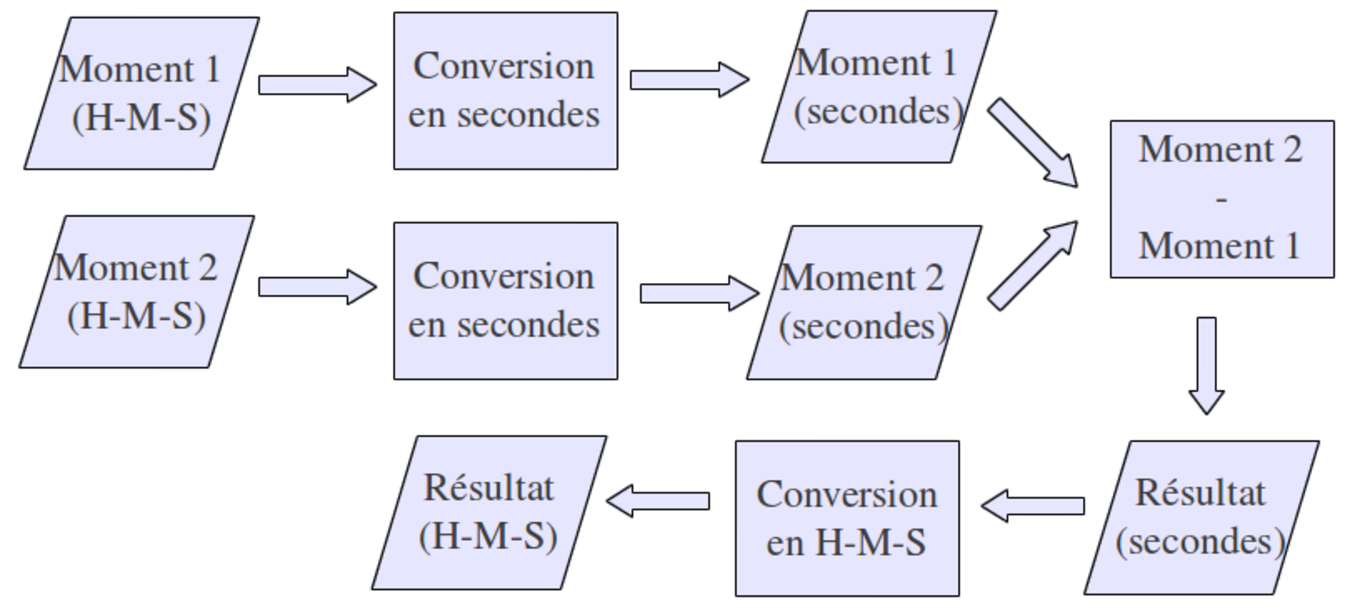
\includegraphics[width=0.8\textwidth]{image/module-conversion}
	\end{center}

\subsection*{Conversion en secondes}

	Une des sous-tâches est donc la conversion en secondes
	d'un moment exprimé en heures-minutes-secondes
	(H-M-S). Il nous faut adapter la solution trouvée pour
	l'exercice du chapitre sur les algorithmes séquentiels
	car il n'est pas question ici que les données soient
	lues ni que le résultat soit écrit ; l'interaction ne
	se fait pas avec l'utilisateur mais avec le module
	principal qui va l'utiliser.\footnote{On pourrait,
	dans notre cas précis, imaginer que le module de conversion demande les
	données à l'utilisateur mais un tel module serait
	moins souvent réutilisable.}

	La première question à se poser est donc celle des paramètres :

	\begin{liste}
	\item 
		Quelles sont les données dont a besoin l'algorithme
		pour travailler ?
	\item 
		Quels résultats fournit-il ?
	\end{liste}

	Dans notre cas, la réponse est simple :

	\begin{liste}
	\item {
		Les données sont le moment à convertir en secondes. Ce moment est
		représenté par trois entiers : les heures, les minutes et les secondes
		;}
	\item {
		Le résultat est le moment converti en secondes. Il est représenté par un
		entier.}
	\end{liste}

	Lorsque le résultat est représenté par une seule donnée, on a le choix
	entre un paramètre en sortie :

	\cadre{
	\begin{pseudo}
		\ModuleSign{HMSversSec}{H\In,M\In,S\In,secondes\Out : entiers}{}
	\end{pseudo}
	}
	
	ou une valeur de retour :

	\cadre{
	\begin{pseudo}
		\ModuleSign{HMSversSec}{H\In,M\In,S\In : entiers}{entier}
	\end{pseudo}
	}

	Dans de pareils cas, 
	on privilégie souvent la valeur de retour car cela
	facilite l'écriture lors de l'appel.

	L'algorithme s'écrit alors :

	\cadre{
	\begin{pseudo}
		\Module{HMSversSec}{H\In,M\In,S\In : entiers}{entier}
			\Decl secondes : entier \RComment A déclarer puisque ce n'est pas un paramètre
			\Let secondes \Gets  H * 3600 + M * 60 + S
			\Return secondes
		\EndModule
	\end{pseudo}
	}

	ou de manière équivalente mais plus concise :

	\cadre{
	\begin{pseudo}
		\Module{HMSversSec}{H\In,M\In,S\In : entiers}{entier}
			\Return H * 3600 + M * 60 + S
		\EndModule
	\end{pseudo}
	}

\subsection{Conversion en heures-minutes-secondes}

	À la fin de notre algorithme, il nous faudra reconvertir un résultat
	exprimé en secondes sous la forme heures-minutes-secondes. À nouveau,
	on a déjà résolu ce problème dans le chapitre sur les algorithmes
	séquentiels. Mais il faut l'adapter à
	l'usage de paramètres.

	\begin{liste}
	\item {
		Quelles sont les données ? Une seule, le moment exprimé en secondes}
	\item {
		Quels sont les résultats calculés par le module ? Ce même moment exprimé
		en heures-minutes-secondes. Trois entiers sont requis ce qui fait que
		le choix entre un paramètre en sortie et une valeur de retour ne se
		pose pas ici ; impossible d'utiliser une valeur de
		retour (qui doit être unique) ; on doit utiliser des paramètres en
		sortie.}
	\end{liste}

	Ce qui donne :

	\cadre{
	\begin{pseudo}
		\Module{secVersHMS}{secondes\In,S\Out,M\Out,S\Out : entiers}{}
			\Let H \Gets secondes DIV 3600
			\Let M \Gets secondes MOD 3600 DIV 60
			\Let S \Gets secondes MOD 60
		\EndModule
	\end{pseudo}
	}

\subsection{La solution}

	À présent, on a tout pour écrire la solution à notre problème

	\cadre{
	\begin{pseudo}
		\Module{différenceEntreHeures}{}{} \RComment Pas de paramètres !
			\Decl H1, M1, S1, H2, M2, S2 : entiers \RComment Les 2 moments à soustraire
			\Decl secondes1, secondes2 : entiers \RComment Ces 2 moments en secondes
			\Decl diffSecondes : entier \RComment La différence en secondes
			\Decl diffH, diffM, diffS : entiers \RComment La différence en H-M-S
			\Read H1, M1, S1, H2, M2, S2
			\Let secondes1 \Gets HMSversSec( H1, M1, S1 )
			\Let secondes2 \Gets HMSversSec( H2, M2, S2 )
			\Let diffSecondes \Gets secondes2 – secondes1
			\Stmt secVersHMS( diffSecondes, diffH, diffM, diffS )
			\Write diffH, diffM, diffS
		\EndModule
	\end{pseudo}
	}

	
	\begin{Emphase}[reflexion]{Variante}
		Dans la solution ci-dessus, 
		quelle est ou quelles sont la/les variable(s) locale(s) 
		dont on pourrait se passer moyennant une réécriture de
		l'algorithme ?
	\end{Emphase}
	
\section{Blocs}

	{
	{Un bloc est l’écriture d’une portion de module
	à l’extérieur de celui-ci. C’est un simple
	}{\textit{déplacement}}{
	de lignes de codes vers un autre endroit du texte de
	l'algorithme. La raison de découper un module en blocs
	peut être le souci de clarifier un algorithme en le découpant en étapes
	bien distinctes, ou tout simplement un manque de place… Les variables
	d’un bloc ne sont donc pas des variables locales du bloc dans lequel
	elles apparaissent, mais bien des variables locales du module auquel
	appartient ce bloc. L’appel de l’exécution des instructions se trouvant
	dans un bloc est similaire à celui d’un module avec paramètres, on
	écrit simplement le nom du bloc comme s’il s’agissait d’une
	instruction.}}

	{
	Pour exemple, le module additionnerFractions (première version dans le
	chapitre 3) pourrait se découper ainsi :}

	\cadre{
	\begin{pseudo}
		\Module{additionnerFractions}{}{}
			\Stmt déclaration
			\Stmt lectureDonnées
			\Stmt calculs
			\Stmt écritureRésultat
		\EndModule
	\end{pseudo}
	}

	\cadre{
	\begin{pseudo}
	\Block{declaration}
		\Decl num1, den1, num2, den2, numRes, denRes : entiers
	\EndBlock
	\end{pseudo}
	}

	\cadre{
	\begin{pseudo}
	\Block{lectureDonnées}
		\Read num1, den1, num2, den2
	\EndBlock
	\end{pseudo}
	}

	\cadre{
	\begin{pseudo}
	\Block{calculs}
		\Let numRes \Gets num1 * den2 + num2 * den1
		\Let denRes \Gets den1 * den2
	\EndBlock
	\end{pseudo}
	}

	\cadre{
	\begin{pseudo}
	\Block{écritureRésultat}
		\Write numRes, "/", denRes \RComment la fraction n'est pas simplifiée
	\EndBlock
	\end{pseudo}
	}

	{
	{Le bloc contenant la déclaration des variables
	est aussi appelé }{\textbf{dictionnaire des
	variables}}{ du module.}}

\section{Qu'est-ce qu'un algorithme de qualité ?}

	{
	Nous voulons tous produire du code de qualité mais
	qu'est-ce que cette notion recouvre vraiment ?
	Qu'est-ce qui permet de juger de la qualité
	d'un code ? De nombreux critères existent. Citons ici,
	parmi les plus pertinents, ceux qui sont le plus liés à ce
	cours\footnote{Pour approfondir cette notion,
	l'étudiant pourra lire par exemple : Bertrand Meyer,
	«~\textit{Conception et programmation par objets : pour du logiciel de
	qualité}~», aux éditions «\textit{~interéditions~}»}. }

\subsection{La validité}

	{
	C'est l'évidence, le code doit
	réaliser les tâches pour lesquelles il a été écrit, même dans tous les
	cas particuliers imaginés. C'est là le critère
	principal et les autres ne sont là que pour aider à atteindre celui-ci
	plus facilement. Ne nous leurrons pas, ce critère est loin
	d'être facile à rencontrer. Il suffit pour
	s'en convaincre de se rappeler toutes les fois où des
	logiciels pourtant courants que nous utilisons se sont déjà arrêtés sur
	des erreurs.}

\subsection{L'extensibilité (ou évolutivité)}

	{
	Un code valide résout un problème particulier. Mais dans les situations
	réelles, le problème change régulièrement. Nous voudrons adapter le
	logiciel à de nouveaux besoins, à une modification de la législation,
	parce qu’un besoin était mal compris, ... Ces modifications peuvent
	parfois être prévues mais pas toujours.}

	{
	Le code doit être écrit de telle sorte qu'un changement
	mineur dans le problème n'implique
	qu'un changement mineur dans le code. Ce changement
	doit être évident, facile à opérer et rapide. Il ne doit pas mettre à
	mal la validité du code.}

\subsection{La réutilisabilité}

	{
	On désigne ici la capacité à réutiliser un bout de code
	d'un projet dans un autre projet. Cette réutilisation
	doit être aisée et sûre. Réutiliser du code permet
	d'utiliser du code qui a déjà été éprouvé et de gagner
	du temps que l'on pourra utiliser à améliorer le code
	que l'on doit encore écrire. La découpe en modules
	joue ici un rôle essentiel.}

\subsection{La lisibilité}

	{
	La lisibilité d'un code recouvre une notion globale et
	locale. Au niveau global, on doit facilement comprendre la structure
	générale du code afin de pouvoir aisément comprendre où se trouve le
	code qui nous intéresse. Au niveau local, on doit pouvoir comprendre
	aisément chaque bout de code.}

	{
	Au niveau du procédural (on nomme ainsi la programmation qui se
	structure à l'aide de modules), cela revient à dire
	qu'on doit rapidement voir quels sont les fonctions et
	leur rôle (niveau global) et que chaque fonction sera aisément
	compréhensible (niveau local). }
	
	{
	Est-ce que la lisibilité d'un code passe par
	l'abondance de commentaire ? Non, pas forcément. Le
	commentaire sert à expliquer ce qui n'est pas
	immédiatement clair dans le code. La première source de lisibilité
	provient donc du code lui-même. C'est pourquoi on est
	attentif à la bonne découpe en modules, au choix judicieux des noms de
	modules et de variables, ... Le respect de ces bonnes pratiques diminue
	le besoin de commentaires.}
	
\subsection{L'efficience}

	{
	Ce critère s'intéresse à la bonne utilisation des
	ressources informatiques. Est ce qu'il va tourner
	suffisamment vite, utiliser peu de mémoire ? Faut-il chercher
	systématiquement à optimiser son code ? Non ! On a souvent tendance à
	surévaluer ce critère ce qui est dommageable pour trois raisons.}

	\begin{liste}
	\item {
		Souvent, l'approche directe est suffisante. Par
		exemple, la plupart des applications sont interactives.
		C'est alors l’utilisateur qui est le plus lent, pas la
		machine qui a tout le temps d'effectuer sa tâche
		pendant que l’utilisateur réfléchit à ce qu'il doit
		taper.}
	\item {
		En général, un programme passe 80\% de son temps dans 20\% de son code.
		Chercher à optimiser chaque ligne de code est une perte de temps.}
	\item {
		Accroitre la rapidité d'un code est presque toujours en
		contradiction avec sa lisibilité. On va utiliser un algorithme moins
		connu ou des raccourcis difficiles à suivre.}
	\end{liste}

	{
	C'est pourquoi on recommande en général, face à un
	problème, d'utiliser la solution la plus courante, la
	plus claire. Une fois le programme terminé, et seulement si le besoin
	s'en fait sentir, on identifiera les portions de code
	où le programme s'attarde le plus et on cherchera à
	les optimiser.}

\section{Exercices}

\begin{Exercice}{Compréhension}
	Indiquer quels nombres sont successivement affichés lors de l’exécution
	des modules ex1, ex2, ex3 et ex4.

	\cadre{
	\begin{pseudo}
	\Module{ex1}{}{}
		\Decl x, y : entiers
		\Stmt addition( 3, 4, x )
		\Write x
		\Let x \Gets 3
		\Let y \Gets 5
		\Stmt addition( x, y, y )
		\Write y
	\EndModule

	\Empty

	\Module{addition}{a\In,b\In,c\Out: entiers}{}
		\Decl somme : entier
		\Let somme \Gets a + b
		\Let c \Gets somme
	\EndModule
	\end{pseudo}
	}

	\cadre{
	\begin{pseudo}
	\Module{ex2}{}{}
		\Decl a, b : entiers
		\Stmt addition( 3, 4, a ) \Comment voir ci-dessus
		\Write a
		\Let a \Gets 3
		\Let b \Gets 5
		\Stmt addition( b, a, b )
		\Write b
	\EndModule
	\end{pseudo}
	}

	\cadre{
	\begin{pseudo}
	\Module{ex3}{}{}
		\Decl a, b, c : entiers
		\Stmt calcul( 3, 4, c )
		\Write c
		\Let a \Gets 3
		\Let b \Gets 4
		\Let c \Gets 5
		\Stmt calcul( b, c, a )
		\Write a, b, c
	\EndModule
	\Empty
	\Module{calcul}{a\In,b\In,c\Out: entiers}{}
		\Let a \Gets 2 * a
		\Let b \Gets 3 * b
		\Let c \Gets a + b
	\EndModule
	\end{pseudo}
	}

	\cadre{
	\begin{pseudo}
	\Module{ex4}{}{}
		\Decl a, b, c : entiers
		\Let a \Gets 3
		\Let b \Gets 4
		\Let c \Gets f(b)
		\Write c
		\Stmt calcul2(a, b, c)
		\Write a, b, c
	\EndModule
	\Empty
	\Module{calcul2}{a\In,b\In,c\Out: entiers}{}
		\Let a \Gets f(a)
		\Let c \Gets 3 * b
		\Let c \Gets a + c
	\EndModule
	\Empty
	\Module{f}{a\In: entier}{entier}
		\Decl b : entier
		\Let b \Gets 2 * a + 1
		\Return b
	\EndModule
	\end{pseudo}
	}

\end{Exercice}

\begin{Exercice}{Appels de module}
	Parmi les instructions suivantes (où les variables
	\textstyleCodeInsr{a}, \textstyleCodeInsr{b} et \textstyleCodeInsr{c}
	sont des entiers), lesquelles font correctement appel au module
	d’en-tête suivant ?

	\cadre{
	\begin{pseudo}
		\ModuleSign{PGCD}{a\In,b\In: entiers}{entier}
	\end{pseudo}
	}

	\cadre{
	\begin{pseudo}
	\Stmt [1] a \Gets PGCD( 24, 32 )
	\Stmt [2] a \Gets PGCD( a, 24 )
	\Stmt [3] b \Gets 3 * PGCD( a + b, 2*c ) + 120
	\Stmt [4] PGCD( 20, 30)
	\Stmt [5] a \Gets PGCD( a, b, c )
	\Stmt [6] a \Gets PGCD( a, b ) + PGCD( a, c )
	\Stmt [7] a \Gets PGCD( a, PGCD( a, b ) )
	\Stmt [8] \K{lire} PGCD( a, b )
	\Stmt [9] \K{écrire} PGCD( a, b)
	\Stmt [10] PGCD(a, b ) \Gets c
	\end{pseudo}
	}
\end{Exercice}

\begin{Exercice}{Comparaison d'algorithmes}
	Soit un module testant si un nombre entier est pair.
	Comparez les différentes solutions proposées.

	\cadre{
	\begin{pseudo}
		\Module{estPair}{nb\In: entier}{booléen}
		\Decl pair : booléen
		\Let pair \Gets faux
		\If{nb MOD 2 = 0}
			\Let pair \Gets vrai
		\EndIf
		\Return pair
		\EndModule
	\end{pseudo}
	}

	\cadre{
	\begin{pseudo}
		\Module{estPair}{nb\In: entier}{booléen}
		\Decl pair : booléen
		\If{nb MOD 2 = 0}
			\Let pair \Gets vrai
		\Else
			\Let pair \Gets faux
		\EndIf
		\Return pair
		\EndModule
	\end{pseudo}
	}

	\cadre{
	\begin{pseudo}
		\Module{estPair}{nb\In: entier}{booléen}
		\Decl pair : booléen
		\Let pair \Gets nb MOD 2 = 0
		\Return pair
		\EndModule
	\end{pseudo}
	}

	\cadre{
	\begin{pseudo}
		\Module{estPair}{nb\In: entier}{booléen}
		\Return nb MOD 2 = 0
		\EndModule
	\end{pseudo}
	}

	\cadre{
	\begin{pseudo}
		\Module{estPair}{nb\In: entier}{booléen}
		\If{nb MOD 2 = 0}
			\Return vrai
		\Else
			\Return faux
		\EndIf
		\EndModule
	\end{pseudo}
	}

	\cadre{
	\begin{pseudo}
		\Module{estPair}{nb\In: entier}{booléen}
		\If{nb MOD 2 = 0}
			\Return vrai
		\EndIf
		\Return faux
		\EndModule
	\end{pseudo}
	}
	
\end{Exercice}

\begin{Exercice}{Échange de variables}
\marginicon{java}
Écrire un module \textit{swap} qui échange le contenu des deux variables
entières passées en paramètres.
\end{Exercice}

\begin{Exercice}{Valeur absolue}
Écrire un module qui retourne la valeur absolue d'un
réel reçu en paramètre.
\end{Exercice}

\begin{Exercice}{Maximum de 4 nombres}
\marginicon{java}
Écrire un module qui retourne le maximum de 4
nombres donnés en paramètres.
\end{Exercice}

\begin{Exercice}{Validité d'une date}
\marginicon{java}
Reprendre l'algorithme de validation d'une date 
développé au chapitre précédent et le rendre modulaire.
\end{Exercice}


% ==================================
\chapter{Les variables structurées}
% ==================================

% ==========================
\section{Le type structuré}
% ==========================

	Dans les chapitres précédents, nous avons utilisé des variables de types
	dits «~simples~» (entier, réel, booléen, caractère, chaine) ne pouvant
	contenir qu’une seule valeur à la fois. Cependant, certains types
	d’information consistent en un regroupement de plusieurs données
	élémentaires. Quelques exemples :

	\begin{liste}
	\item {
		une \textbf{date} est composée de trois éléments (le jour, le mois,
		l’année), le mois s’exprimant tantôt par un entier (15/10/2004) tantôt
		par une chaine (15 octobre 2004)}
	\item {
		un \textbf{moment} de la journée est un triple d’entiers (heures,
		minutes, secondes)}
	\item {
		la localisation d’un \textbf{point} dans un plan nécessite la
		connaissance de deux coordonnées cartésiennes (l’abscisse \textit{x} et
		l’ordonnée \textit{y}) ou polaires (le rayon \textit{r} et l’angle
		\textit{$\theta $})}
	\item {
		une \textbf{adresse }est composée de plusieurs données : un nom de rue,
		un numéro de maison, parfois un numéro de boite postale, un code
		postal, le nom de la localité, un nom ou code de pays pour une adresse
		à l’étranger\dots}
	\end{liste}

	Pour stocker et manipuler de tels ensembles de données, nous utiliserons
	des \textbf{types structurés} ou \textbf{structures}\footnote{Nous
	verrons dans un chapitre ultérieur que l'approche
	«~orienté objet~» offre également une solution élégante pour manipuler
	des données complexes}. Une \textbf{structure} est donc un ensemble
	fini d’éléments pouvant être de types distincts. Chaque élément de cet
	ensemble, appelé \textbf{champ} de la structure, possède un nom unique.
	
	Noter qu’un champ d’une structure peut lui-même être une structure. Par
	exemple, une \textbf{carte d’identité} inclut parmi ses informations
	une \textbf{date} de naissance, l’\textbf{adresse} de son
	propriétaire\dots

% ===================================
\section{Définition d'une structure}
% ===================================

	\marginicon{definition}
	La définition d’un type structuré adoptera le modèle suivant :

	\cadre{
	\begin{pseudo}
	\Struct{NomDeLaStructure}
		\Decl nomChamp1 : type1
		\Decl nomChamp2 : type2
		\Decl \dots
		\Decl nomChampN : typeN
	\EndStruct
	\end{pseudo}
	}

	nomChamp1, \dots, nomChampN 
	sont les noms des différents champs de la structure, 
	et type1, \dots, typeN les types de ces champs. 
	Ces types sont soit les types «~simples~» étudiés
	précédemment (entier, réel, booléen, caractère, chaine) soit d’autres
	types structurés dont la structure aura été préalablement définie.

	Pour exemple, nous définissons ci-dessous trois
	types structurés que nous utiliserons souvent par la suite :

	\cadre{
	\begin{pseudo}
	\Struct{Date}
		\Decl jour : entier
		\Decl mois : entier
		\Decl année : entier
	\EndStruct
	\end{pseudo}
	}

	\cadre{
	\begin{pseudo}
	\Struct{Moment}
		\Decl heure : entier
		\Decl minute : entier
		\Decl seconde : entier
	\EndStruct
	\end{pseudo}
	}

	\cadre{
	\begin{pseudo}
	\Struct{Point}
		\Decl x : réel
		\Decl y : réel
	\EndStruct
	\end{pseudo}
	}

% =====================================================
\section{Déclaration d’une variable de type structuré}
% =====================================================

	Une fois un type structuré défini, la
	déclaration de variables de ce type est identique à celle des variables
	simples. Par exemple :

	\cadre{
	\begin{pseudo}
	\Decl anniversaire, jourJ : Date
	\Decl départ, arrivée, unMoment : Moment
	\Decl a, b, centreGravité : Point
	\end{pseudo}
	}

% ====================================================
\section{Utilisation des variables de type structuré}
% ====================================================

	En général, pour manipuler une variable
	structurée ou en modifier le contenu, il faut agir au niveau de ses
	champs en utilisant les opérations permises selon leur type. Pour
	accéder à l’un des champs d’une variable structurée, il faut mentionner
	le nom de ce champ ainsi que celui de la variable dont il fait partie.
	Nous utiliserons la notation «~pointée~» :

	\cadre{
	\begin{pseudo}
	\Stmt nomVariable.nomChamp
	\end{pseudo}
	}

	Exemple d’instructions utilisant les variables
	déclarées au paragraphe précédent :

	\cadre{
	\begin{pseudo}
	\Let anniversaire.jour \Gets 15
	\Let anniversaire.mois \Gets 10
	\Let anniversaire.année \Gets 2014
	\Let arrivée.heure \Gets départ.heure+2
	\Let centreGravité.x \Gets (a.x+b.x)/2
	\end{pseudo}
	}

	On peut cependant dans certains cas utiliser
	une variable structurée de manière globale (c’est-à-dire d’une façon
	qui agit simultanément sur chacun de ses champs). Le cas le plus
	courant est l’affectation interne entre deux variables structurées de
	même type, par exemple :

	\cadre{
	\begin{pseudo}
	\Let arrivée \Gets départ
	\end{pseudo}
	}

	qui résume les trois instructions suivantes :

	\cadre{
	\begin{pseudo}
	\Let arrivée.heure \Gets départ.heure
	\Let arrivée.minute \Gets départ.minute
	\Let arrivée.seconde \Gets départ.seconde
	\end{pseudo}
	}

	Une variable structurée peut aussi être le
	paramètre d’un module, et un module peut également renvoyer une
	«~valeur~» de type structuré. Par exemple, l’en-tête d’un module
	renvoyant le nombre de secondes écoulées entre une heure de départ et
	d’arrivée serait :

	\cadre{
	\begin{pseudo}
	\ModuleSign{nbSecondesEcoulées}{ départ\In, arrivée\In : Moment}{entier}
	\end{pseudo}
	}

	On pourra aussi lire ou afficher une variable structurée\footnote{Bien que, dans certains
	langages, ces opérations devront être décomposées en une lecture ou
	écriture de chaque champ de la structure.}.

	\cadre{
	\begin{pseudo}
	\Read unMoment
	\Write unMoment
	\end{pseudo}
	}

	Par contre, il n’est pas autorisé d’utiliser
	les opérateurs de comparaison ({\textless}, {\textgreater}) pour
	comparer des variables structurées (même de même type), car une
	relation d’ordre n’accompagne pas toujours les structures utilisées. En
	effet, s’il est naturel de vouloir comparer des dates ou des moments,
	comment définir une relation d’ordre avec les points du plan ou avec
	des cartes d’identités ?

	Si le besoin de comparer des variables
	structurées se fait sentir, il faudra dans ce cas écrire des modules de
	comparaison adaptés aux structures utilisées.

	Par facilité, on peut assigner tous les champs en une fois via des
	«~\{\}~». Exemple :

	\cadre{
	\begin{pseudo}
	\Let anniversaire \Gets \{1,9,1989\}
	\end{pseudo}
	}

% =============================
\section{Exemple d’algorithme}
% =============================

	Le module ci-dessous reçoit en paramètre deux dates ; la valeur renvoyée
	est –1 si la première date est antérieure à la deuxième, 0 si les deux
	dates sont identiques ou 1 si la première date est postérieure à la
	deuxième.

	\cadre{
	\begin{pseudo}
	\Module{comparerDates}{date1\In, date2\In}{entier}
		\Decl résultat : entier
		\Let  résultat \Gets -1
		\If{date1.année ${\geq}$ date2.année}
			\If{date1.année $>$ date2.année}
				\Let  résultat \Gets 1
			\Else \RComment Les années sont identiques
				\If{date1.mois ${\geq}$ date2.mois}
					\If{date1.mois $>$ date2.mois}
						\Let  résultat \Gets 1
					\Else \RComment Les mois sont identiques
						\If{date1.jour ${\geq}$ date2.jour}
							\If{date1.jour $>$ date2.jour}
								\Let  résultat \Gets 1
							\Else \RComment Les jours sont identiques
								\Let  résultat \Gets 0
							\EndIf
						\EndIf
					\EndIf
				\EndIf
			\EndIf
		\EndIf
		\Return résultat
	\EndModule
	\end{pseudo}
	}

% =====================================
\section{Exercices sur les structures}
% =====================================

\begin{Exercice}{Conversion moment-secondes}
	Écrire un module qui reçoit en paramètre un
	moment d’une journée et qui retourne le nombre de secondes écoulées
	depuis minuit jusqu’à ce moment.
\end{Exercice}

\begin{Exercice}{Conversion secondes-moment}
	Écrire un module qui reçoit en paramètre un
	nombre de secondes écoulées dans une journée à partir de minuit et qui
	retourne le moment correspondant de la journée.
\end{Exercice}

\begin{Exercice}{Temps écoulé entre 2 moments}
	Écrire un module qui reçoit en paramètres deux
	moments d’une journée et qui retourne le nombre de secondes séparant
	ces deux moments.
\end{Exercice}

\begin{Exercice}{Milieu de 2 points}
	Écrire un module recevant les coordonnées de
	deux points distincts du plan et retournant les coordonnées du point
	situé au milieu des deux.
\end{Exercice}

\begin{Exercice}{Distance entre 2 points}
	Écrire un module recevant les coordonnées de
	deux points distincts du plan et qui retourne
	la distance entre ces deux points.
\end{Exercice}

\begin{Exercice}{Un rectangle}
	\marginicon{java}
	Définir un type \textbf{Rectangle} pouvant décrire de façon
	commode un rectangle dans un espace à deux dimensions et dont les côtés
	sont parallèles aux axes des coordonnées. 
	Écrire ensuite

	\begin{enumerate}[label=\alph*)]
	\item {
		un module calculant le périmètre d’un rectangle reçu en paramètre ;}
	\item {
		un module calculant la surface d’un rectangle reçu en paramètre ;}
	\item {
		un module recevant en paramètre un rectangle R et les coordonnées
		d'un point P, et renvoyant 
		\textbf{vrai} si et seulement si le point P est à
		l'intérieur du rectangle R ;}
	\item {
		un module recevant en paramètre un rectangle R et les coordonnées
		d'un \ point P, et renvoyant 
		\textbf{vrai} si et seulement si le point P est sur le bord du
		rectangle R ;}
	\item {
		un module recevant en paramètre deux rectangles et renvoyant la valeur
		booléenne \textbf{vrai} si et seulement si ces deux rectangles ont une
		intersection.}
	\end{enumerate}
\end{Exercice}

\begin{Exercice}{Un cercle}
	Définir un type \textbf{Cercle} pouvant décrire de façon
	commode un cercle quelconque dans un espace à deux dimensions. 
	Écrire ensuite
	
	\begin{enumerate}[label=\alph*)]
	\item {
		un module calculant la surface du cercle reçu en paramètre ;}
	\item {
		un module recevant 2 points en paramètre et retournant le cercle dont le
		diamètre est défini par ces 2 points ;}
	\item {
		un module qui détermine si un point donné est dans un cercle ;}
	\item {
		un module qui indique si 2 cercles ont une intersection.
	}
	\end{enumerate}
\end{Exercice}

\begin{Exercice}{Validation de date}
	Écrire un algorithme qui valide une date reçue en paramètre 
	sous forme d'une structure.
\end{Exercice}

	

% ====================
\chapter{Les boucles}
\label{chap:bcl}
% ====================

	\marginicon{objectif}
	Les ordinateurs révèlent tout leur potentiel dans leur capacité à
	répéter inlassablement les mêmes tâches. Nous voyons ici comment
	spécifier des boucles dans nos codes et comment les utiliser à bon
	escient.

	\marginicon{attention}
	Attention ! D'expérience, nous savons que ce chapitre
	est difficile à appréhender par les étudiants. Beaucoup
	d'entre-vous perdent pied ici. Accrochez-vous et
	faites bien tous les exercices proposés !


% =======================================
\section{La notion de travail répétitif}
% =======================================

	Si on veut faire effectuer un travail répétitif, 
	il faut indiquer deux choses
	
	\begin{enumerate}
	\item Le travail à répéter
	\item Comment savoir s'il faut continuer la répétition 
		ou l'arrêter.
	\end{enumerate}

	Examinons quelques exemples pour fixer notre propos.

	\textbf{Exemple 1} : Pour traiter des dossiers, on dira quelque chose
	comme «~tant qu'il reste un dossier à traiter, le
	traiter~» ou encore «~traiter un dossier puis passer au suivant
	jusqu'à ce qu'il
	n'en reste plus à traiter~».

	\begin{liste}
	\item La tâche à répéter est : «~traiter un dossier~»
	\item On indique qu'on doit continuer s'il
		reste encore un dossier à traiter
	\end{liste}

	\textbf{Remarque :} On aurait aussi pu le formuler ainsi : «~traiter un
	dossier et passer au suivant jusqu'à ce
	qu'il n'en reste plus~»

	\textbf{Exemple 2} : Pour calculer la cote finale de tous les étudiants,
	on aura quelque chose du genre «~Pour tout étudiant, calculer sa
	cote~»

	\begin{liste}
	\item 
		La tâche à répéter est : «~calculer la cote d'un
		étudiant~»
	\item 
		On indique qu'on doit le faire pour tous les étudiants.
		On doit donc commencer par le premier, passer à chaque fois au suivant
		et s'arrêter quand on a fini le dernier.
	\end{liste}

	\textbf{Exemple 3} : Pour afficher tous les nombres de 1 à 100, on aura
	«~Pour tous les nombres de 1 à 100, afficher ce nombre~»

	\begin{liste}
	\item
		La tâche à répéter est : «~afficher un nombre~»
	\item 
		On indique qu'on doit le faire pour tous les nombres de
		1 à 100. On doit donc commencer avec 1, passer à chaque fois au nombre
		suivant et s'arrêter après avoir affiché le nombre
		100.
	\end{liste}

	\textbf{Attention} ! Comprenez bien que c'est toujours
	la même tâche qui est exécutée mais pas avec le même effet à chaque
	fois. Ainsi, on traite un dossier mais à chaque fois un différent; on
	affiche un nombre mais à chaque fois un différent. Nous verrons comment
	y arriver en logique.

% ==============================
\section{Structures itératives}
% ==============================

	Chacune des structures suivantes traduit une volonté de faire exécuter
	un certain nombre de fois une séquence d’instructions. 

	\subsection{«~tant que~»}

		Le «~tant que~» est une structure qui demande à
		l'exécutant de répéter une tâche (une ou plusieurs
		instructions) tant qu'une condition donnée est vraie.

		\cadre{
		\begin{pseudo}
		\While{condition}
			\Stmt séquence d’instructions à exécuter
		\EndWhile
		\end{pseudo}
		}

		Comme pour la structure \textstyleMotCl{si}, la \textbf{condition} est
		une expression à valeur booléenne. Dans ce type de structure, il faut
		qu’il y ait dans la séquence d’instructions comprise entre
		\textstyleMotCl{tant que} et \textstyleMotCl{fin tant que} au moins une
		instruction qui modifie une des composantes de la condition de telle
		manière qu’elle puisse devenir \textbf{fausse} à un moment donné
		(sinon, boucle infinie!). La figure \vref{fig:boucle-tq} donne 
		un ordinogramme mettant en évidence la dynamique de cette structure. 
		On remarquera que si la condition est fausse dès le début, 
		la tâche n'est jamais exécutée.

		\begin{figure}[h]
		\centering
		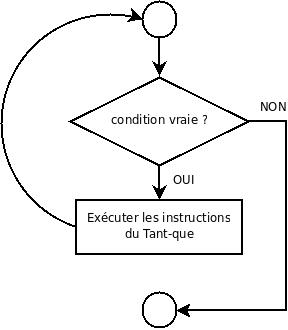
\includegraphics[width=0.5\textwidth]{image/boucle-tq}
		\caption{Ordinogramme de la boucle "tant-que"}
		\label{fig:boucle-tq}
		\end{figure}
		
	\subsection{«~faire – jusqu'à ce que~»}

		Cette structure est très proche du «~tant que~» 
		à deux différences près :
	
		\begin{enumerate}
		\item {
			Le test est fait à la fin et pas au début. La tâche est donc toujours
			exécutée au moins une fois. }
		\item {
			On donne la condition pour arrêter et pas pour continuer; il
			s'agit d'une différence mineure.}
		\end{enumerate}

		\cadre{
		\begin{pseudo}
		\Repeat
			\Stmt séquence d’instructions à exécuter
		\Until{condition}
		\end{pseudo}
		}

		Comme ci-dessus, il faut que la séquence d’instructions comprise entre
		\textstyleMotCl{faire} et \textstyleMotCl{jusqu'à ce
		que} contienne au moins une instruction qui modifie la condition de
		telle manière qu’elle puisse devenir \textbf{vraie} à un moment donné
		pour arrêter l'itération. 
		La figure \vref{fig:boucle-faire} donne 
		un ordinogramme mettant en évidence la dynamique de cette structure. 

		\begin{figure}[h]
		\centering
		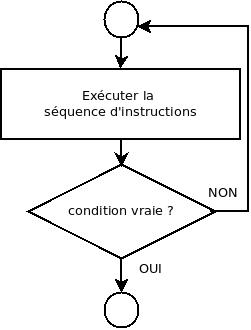
\includegraphics[width=0.4\textwidth]{image/boucle-faire}
		\caption{Ordinogramme de la boucle "faire – jusqu'à ce que"}
		\label{fig:boucle-faire}
		\end{figure}

	\subsection{«~pour~»}

		Ici, on va plutôt indiquer \textbf{combien de fois} la tâche doit être
		répétée. Cela se fait au travers d'une
		\textbf{variable de contrôle} dont la valeur va évoluer à partir
		d'une valeur de départ jusqu'à une
		valeur finale.
		
		\cadre{
		\begin{pseudo}
		\For{variable \K{de} début \K{à} fin [\K{par} pas]}
			\Stmt séquence d’instructions à exécuter
		\EndFor
		\end{pseudo}
		}

		Dans ce type de structure, \textbf{début}, \textbf{fin} et \textbf{pas}
		peuvent être des constantes, des variables ou des expressions (le plus
		souvent à valeurs entières mais on admettra aussi des réels). Le
		\textbf{pas} est facultatif, et généralement omis. Dans ce cas, la
		valeur par défaut est 1. Ce pas est parfois négatif, dans le cas
		d'un compte à rebours, par exemple
		\textstyleCodeInsr{pour n de 10 à 1 par -1}.

		Quand le \textbf{pas} est positif, la boucle s'arrête
		lorsque la variable dépasse la valeur de \textbf{fin}. Par contre, avec
		un \textbf{pas} négatif, la boucle s'arrête lorsque la
		variable prend une valeur plus petite que la valeur de \textbf{fin}
		(cf. le test dans l'organigramme de la figure \vref{fig:boucle-pour})

		\begin{figure}[h]
		\centering
		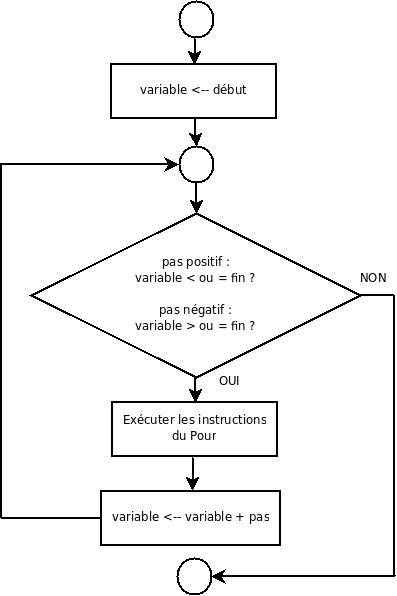
\includegraphics[width=0.5\textwidth]{image/boucle-pour}
		\caption{Ordinogramme de la boucle "pour"}
		\label{fig:boucle-pour}
		\end{figure}

		\marginicon{attention}
		Veiller à la cohérence de l’écriture de cette structure. On considérera
		qu’au cas (à éviter) où \textbf{début} est strictement supérieur à
		\textbf{fin} et le \textbf{pas} est positif, la séquence d’instructions
		n’est jamais exécutée (mais ce n’est pas le cas dans tous les langages
		de programmation !). Idem si \textbf{début} est strictement inférieur à
		\textbf{fin} mais avec un \textbf{pas} négatif.

		\textbf{Exemples~}:

		\cadre{
		\begin{pseudo}
		\Stmt \K{pour} i \K{de} 0 \K{à} 2 \K{faire} \RComment La boucle est exécutée 3 fois.
		\Stmt \K{pour} i \K{de} 2 \K{à} 0 \K{faire} \RComment La boucle n'est pas exécutée.
		\Stmt \K{pour} i \K{de} 1 \K{à} 10 \K{par} -1 \K{faire} \RComment La boucle n'est pas exécutée.
		\Stmt \K{pour} i \K{de} 1 \K{à} 1 \K{par} 5 \K{faire} \RComment La boucle est exécutée 1 fois.
		\end{pseudo}
		}
		
		\marginicon{attention}
		Veiller aussi à ne pas modifier dans la séquence d’instructions une des
		variables de contrôle \textbf{début}, \textbf{fin} ou \textbf{pas} ! Il
		est aussi fortement déconseillé de modifier «~manuellement~» la
		\textbf{variable} de contrôle au sein de la boucle
		\textstyleMotCl{pour}. Il ne faut pas l’initialiser en début de boucle,
		et ne pas s’occuper de sa modification, l’instruction \textbf{variable}
		{\textsf{\textbf{←}}} \textbf{variable} +
		\textbf{pas} étant automatique et implicite à chaque étape de la
		boucle. Il est aussi déconseillé d’utiliser \textbf{variable} à la
		sortie de la structure \textstyleMotCl{pour} sans lui affecter une
		nouvelle valeur (son contenu pouvant varier selon le langage de
		programmation).

	\subsection{Quel type de boucle choisir ?}

		En pratique, il est possible d’utiliser systématiquement la boucle 
		\textstyleMotCl{tant que} qui peut s’adapter à toutes les situations. 
		Cependant, il est plus clair d’utiliser \textstyleMotCl{pour} dans les cas 
		où le nombre d’itérations est fixé et connu à l’avance 
		(par là, on veut dire que le nombre d'itérations est déterminé au moment 
		où on arrive à la boucle). 
		La boucle \textstyleMotCl{faire} convient quant à elle
		dans les cas où le contenu de la boucle doit être parcouru au moins une
		fois, alors que dans \textstyleMotCl{tant que}, 
		le nombre de parcours peut être nul si la condition initiale est fausse. 
		La figure \vref{fig:boucle-choix} propose un petit schéma récapitulatif.

		\begin{figure}[h]
		\centering
		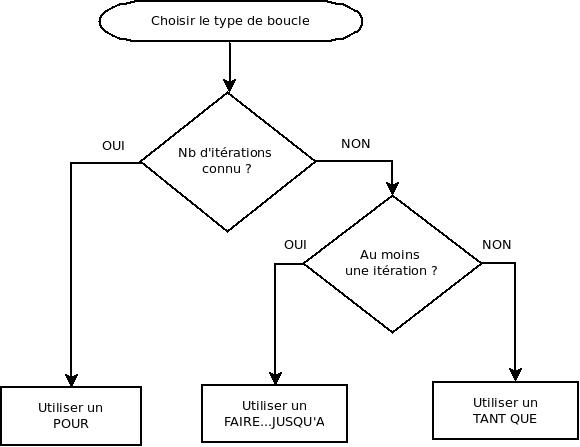
\includegraphics[width=0.7\textwidth]{image/boucle-choixtype}
		\caption{Quel type de boucle choisir ?}
		\label{fig:boucle-choix}
		\end{figure}

% =================
\section{Exemples}
% =================

	Nous présentons quelques exemples de difficulté
	croissante pour montrer comment bien utiliser les boucles.

	\subsection{Exemple 1 -- Compter de 1 à 10}

		Imaginons qu'on veuille afficher tous les nombres de 1 à 10. 
		On va évidemment rejeter cette première solution :

		\cadre{
		\begin{pseudo}
		\Module{compterJusque10}{}{} \RComment Une mauvaise solution !
		\Write 1
		\Write 2
		\Write 3
		\Write 4
		\Write 5
		\Write 6
		\Write 7
		\Write 8
		\Write 9
		\Write 10
		\EndModule
		\end{pseudo}
		}

		Non seulement c'est long à écrire 
		(imaginer l'algorithme pour afficher les nombres de 1 à 10000 !) 
		mais c'est très peu souple.
		Cela ne fonctionne que pour 10 : il faut modifier l'algorithme pour
		un autre décompte. La boucle va nous permettre
		d'obtenir un algorithme qui s'adapte
		à la limite du décompte.

		Posons-nous les bonnes questions pour déterminer la boucle :

		\begin{liste}
		\item 
			Quelle est la tâche à répéter ? Afficher un nombre.
		\item 
			Comment savoir si on continue ? On arrête quand «~10~» est affiché.
		\item 
			Comment afficher à chaque fois un nombre différent ? 
			Au travers d'une variable qui prendra toutes les valeurs de 1 à 10. 
			Il faut donc ajouter dans le corps de la
			boucle une incrémentation de la variable
		\end{liste}

		Ce qui donne :

		\cadre{
		\begin{pseudo}
		\Module{compterJusque10}{}{} \RComment Version avec tant que
			\Decl nb : entier
			\Let nb \Gets 1 \RComment C'est le premier nombre à afficher
			\While{nb $\leq$ 10} \RComment Tant que le nb à afficher est toujours bon
				\Write nb \RComment On affiche la valeur de la variable nb
				\Let nb \Gets nb + 1 \RComment On passe au nombre suivant
			\EndWhile
		\EndModule
		\end{pseudo}
		}

		Mais ici, on pourrait aussi l'écrire avec un «~pour~» vu qu'on
		connait exactement le nombre de passages dans la boucle (10). 
		La variable de contrôle va évoluer de 1 à 10 ce qui tombe bien car
		c'est justement le nombre à afficher à chaque fois.

		\cadre{
		\begin{pseudo}
		\Module{compterJusque10}{}{} \RComment Version avec pour
			\Decl nb : entier
			\For{nb \K{de} 1 \K{à} 10} \RComment Par défaut le pas est de 1
				\Write nb 
			\EndFor
		\EndModule
		\end{pseudo}
		}

		On obtient une solution plus courte et plus lisible 
		car l'en-tête du «~pour~» indique clairement
		comment va évoluer la boucle
		(valeur de départ, pas et valeur finale)

	\subsection{Exemple 2 -- Compter de 1 à beaucoup}

		Dans l'exercice précédent, on a
		affirmé que la boucle pouvait s'adapter à la limite du
		décompte. Montrons-le ! Supposons qu'on veuille
		afficher les nombres de 1 à n où n est une valeur donnée par
		l'utilisateur.

		Rien de plus simple, il suffit de lire cette
		valeur au début et de l'utiliser comme limite de boucle

		\cadre{
		\begin{pseudo}
		\Module{afficherN}{}{} 
			\Decl nb, n : entier
			\Read n
			\For{nb \K{de} 1 \K{à} n} 
				\Write nb 
			\EndFor
		\EndModule
		\end{pseudo}
		}

		\marginicon{reflexion}
		\textbf{Réflexion} : Que se passe-t-il si l'utilisateur entre une valeur négative ?
		Comment améliorer le code pour que le programme
		le signale à l'utilisateur ?

	\subsection{Exemple 3 -- Afficher les nombres pairs}

		Cela se complique un peu. Cette fois-ci on
		affiche uniquement les nombres \textbf{pairs} jusqu'à la limite $n$.
		
		\textbf{Exemple} : 
		les nombres pairs de $1$ à $10$ sont : $2$, $4$, $6$, $8$, $10$.
		
		Notez que $n$ peut être impair. Si $n$ vaut $11$, 
		l'affichage est le même que pour $10$.

		Est-ce qu'on peut utiliser un «~pour~» ? 
		Oui. De 1 à n, il y a exactement «~n DIV 2~» nombres à afficher. 
		La difficulté vient du lien à faire entre la variable de
		contrôle et le nombre à afficher.

		\textbf{Solution 1} : 
		on garde le lien entre la variable de contrôle 
		et le nombre à afficher. 
		Dans ce cas, on commence à $2$ et le pas doit être de $2$.

		\cadre{
		\begin{pseudo}
		\Module{afficherPair}{}{} 
			\Decl nb, n : entier
			\Read n
			\For{nb \K{de} 2 \K{à} n \K{par} 2} 
				\Write nb 
			\EndFor
		\EndModule
		\end{pseudo}
		}

		\textbf{Solution 2} : 
		la variable de contrôle compte simplement le nombre d'itérations.
		Alors il faut calculer le nombre à afficher en fonction de la variable
		de contrôle (ici le double de celle-ci convient)

		\cadre{
		\begin{pseudo}
		\Module{afficherPair}{}{} 
			\Decl i, n : entier
			\Read n
			\For{nb \K{de} 1 \K{à} n DIV 2} 
				\Write 2 * i 
			\EndFor
		\EndModule
		\end{pseudo}
		}

		Par une vieille habitude des programmeurs\footnote{Née avec 
		le langage FORTRAN où la variable $i$ était par défaut une variable entière.},
		une variable de contrôle qui se contente de compter les passages dans
		la boucle est souvent nommée $i$. 
		On l'appelle aussi «~itérateur~».

	\subsection{Exemple 4 -- Afficher les premiers nombres pairs}

		Voici un problème proche du précédent : 
		on affiche cette fois les $N$ premiers nombres pairs.
		
		\textbf{Exemple} : 
		les $10$ premiers nombres pairs sont : $2$, $4$, $6$, $8$, $10$, $12$, $14$, $16$, $18$, $20$.
		
		Il est plus simple de partir de la solution 2 de l'exemple précédent
		en changeant simplement la valeur finale de la boucle.

		\cadre{
		\begin{pseudo}
		\Module{afficherPair}{}{} 
			\Decl i, n : entier
			\Read n
			\For{nb \K{de} 1 \K{à} n} 
				\Write 2 * i 
			\EndFor
		\EndModule
		\end{pseudo}
		}

	\subsection{Exemple 5 -- Somme de nombres}

		Changeons de problème. On veut pouvoir calculer
		la somme d'une série de nombres donnés par
		l'utilisateur. Il faut d'abord se
		demander comment l'utilisateur va pouvoir indiquer
		combien de nombres il faut additionner ou quand est-ce que le dernier
		nombre à additionner a été entré. Voyons quelques possibilités.

		\textbf{Variante 1} : 
		L'utilisateur indique le nombre de termes au départ.
		Ce problème est proche de ce qui a déjà été fait.
		
		\cadre{
		\begin{pseudo}
		\Module{sommeNombres}{}{} \RComment Variante 1
			\Decl nbValeurs : entier \RComment nb de valeurs à additionner
			\Decl valeur : entier \RComment un des termes de l'addition
			\Decl somme : entier \RComment la somme
			\Decl i : entier \RComment itérateur
			\Let somme \Gets 0 \RComment la somme se construit petit à petit. 0 au départ
			\Read nbValeurs
			\For{nb \K{de} 1 \K{à} nbValeurs} 
				\Read valeur
				\Let somme \Gets somme + valeur 
			\EndFor
			\Write somme
		\EndModule
		\end{pseudo}
		}

		\textbf{Variante 2} : Après chaque nombre, 
		on demande à l'utilisateur s'il y a encore un nombre à additionner.

		Ici, il faut chercher une solution différente
		car on ne connait pas au départ le nombre de valeurs à additionner et
		donc le nombre de passages dans la boucle. On va devoir passer à un
		«~tant que~» ou un «faire jusqu'à ce que». On peut
		envisager de demander en fin de boucle s'il reste
		encore un nombre à additionner. Ce qui donne :

		\cadre{
		\begin{pseudo}
		\Module{sommeNombres}{}{} \RComment Variante 2a
			\Decl encore : booléen \RComment est-ce qu'il reste encore une valeur à additionner ?
			\Decl valeur : entier \RComment un des termes de l'addition
			\Decl somme : entier \RComment la somme
			\Let somme \Gets 0
			\Repeat 
				\Read valeur
				\Let somme \Gets somme + valeur 
				\Read encore
			\Until{NON encore}
			\Write somme
		\EndModule
		\end{pseudo}
		}
		
		Avec cette solution, on additionne au moins une valeur. 
		Si on veut pouvoir tenir compte du
		cas très particulier où l'utilisateur ne veut
		additionner aucune valeur, il faut utiliser un «~tant que~» et donc
		poser la question avant d'entrer dans la boucle.

		\cadre{
		\begin{pseudo}
		\Module{sommeNombres}{}{} \RComment Variante 2b
			\Decl encore : booléen \RComment est-ce qu'il reste encore une valeur à additionner ?
			\Decl valeur : entier \RComment un des termes de l'addition
			\Decl somme : entier \RComment la somme
			\Let somme \Gets 0
			\Read encore
			\While{encore} 
				\Read valeur
				\Let somme \Gets somme + valeur 
				\Read encore
			\EndWhile
			\Write somme
		\EndModule
		\end{pseudo}
		}

		\textbf{Variante 3} :
		L'utilisateur entre une valeur spéciale pour indiquer la fin. 
		On parle de valeur \textbf{sentinelle}. 
		Ceci n'est possible que si cette valeur \textbf{sentinelle} ne peut pas être
		un terme valide de l'addition. Par exemple, si on veut
		additionner des nombres positifs uniquement, la valeur -1 peut servir
		de valeur sentinelle. Mais sans limite sur les nombres à additionner
		(positifs, négatifs ou nuls) il n'est pas possible de
		choisir une sentinelle.

		Ici, on se base sur la valeur entrée pour décider si on continue ou pas. 
		Il faut donc \textbf{toujours} effectuer un test
		après une lecture de valeur. C'est pour cela
		qu'il faut effectuer une lecture avant et une autre à
		la fin de la boucle.

		\cadre{
		\begin{pseudo}
		\Module{sommeNombres}{}{} \RComment Variante 3
			\Decl valeur : entier \RComment un des termes de l'addition
			\Decl somme : entier \RComment la somme
			\Let somme \Gets 0
			\Read valeur
			\While{valeur ${\neq}$ -1} 
				\Let somme \Gets somme + valeur 
				\Read valeur \RComment remarquer l'endroit où on lit une valeur.
			\EndWhile
			\Write somme
		\EndModule
		\end{pseudo}
		}

		Voilà ! Vous devriez à présent être en mesure de
		résoudre les exercices qui suivent.
		Courage ! Et n'en passez aucun !

		\marginicon{reflexion}
		\textbf{Réflexion} : 
		Quelle valeur sentinelle prendrait-on 
		pour additionner une série de cotes d'interrogations ? 
		Une série de températures ?

		\textbf{Réflexion} : 
		Dans les solutions 2 et 3 on lit une variable booléenne. 
		Comment un programmeur pourrait-il réaliser 
		cette instruction de façon pratique ?

% ==================
\section{Exercices}
% ==================

\begin{Exercice}{Compréhension d'algorithmes}
	Quels sont les affichages réalisés lors de l'exécution
	des algorithmes suivants ?
	
	\cadre{
	\begin{pseudo}
	\Module{boucle1}{}{}
		\Decl x : entier
		\Let x \Gets 0
		\While{x < 12}
			\Let x \Gets x + 2	
		\EndWhile
		\Write x
	\EndModule
	\end{pseudo}
	}
	
	\cadre{
	\begin{pseudo}
	\Module{boucle2}{}{}
		\Decl ok : booléen
		\Decl x : entier
		\Let ok \Gets vrai
		\Let x \Gets 5
		\While{ok}
			\Let x \Gets x + 7	
			\Let ok \Gets x MOD 11 $\neq$ 0	
		\EndWhile
		\Write x
	\EndModule
	\end{pseudo}
	}

	\cadre{
	\begin{pseudo}
	\Module{boucle3}{}{}
		\Decl ok : booléen
		\Decl cpt, x : entiers
		\Let x \Gets 10
		\Let cpt \Gets 0
		\Let ok \Gets vrai
		\While{ok ET cpt < 3}
			\If{x MOD 2 = 0}
				\Let x \Gets x + 1
				\Let ok \Gets x < 20
			\Else
				\Let x \Gets x + 3
				\Let cpt \Gets cpt + 1
			\EndIf
		\EndWhile
		\Write x
	\EndModule
	\end{pseudo}
	}

	\cadre{
	\begin{pseudo}
	\Module{boucle4}{}{}
		\Decl pair, grand : booléens
		\Decl p, x : entiers
		\Let x \Gets 1
		\Let p \Gets 1
		\Let ok \Gets vrai
		\Repeat
			\Let p \Gets 2 * p
			\Let x \Gets x + p
			\Let pair \Gets x MOD 2 = 0
			\Let grand \Gets x > 15
		\Until{pair OU grand}
		\Write x
	\EndModule
	\end{pseudo}
	}

	\cadre{
	\begin{pseudo}
	\Module{boucle5}{}{}
		\Decl i, x : entiers
		\Decl ok : booléen
		\Let x \Gets 3
		\Let ok \Gets vrai
		\For{i \K{de} 1 \K{à} 5}
			\Let x \Gets x + i
			\Let ok \Gets ok ET (x MOD 2 = 0)
		\EndFor
		\If{ok}
			\Write x
		\Else
			\Write 2 * x
		\EndIf
	\EndModule
	\end{pseudo}
	}

	\cadre{
	\begin{pseudo}
	\Module{boucle6}{}{}
		\Decl i, j, fin : entiers
		\For{i \K{de} 1 \K{à} 3}
			\Let fin \Gets 6 * i - 11
			\For{j \K{de} 1 \K{à} fin \K{par} 3}
				\Write 10 * i + j
			\EndFor
		\EndFor
	\EndModule
	\end{pseudo}
	}

\end{Exercice}
\bigskip
\bigskip
\begin{Exercice}{Simplification}
	Voici quelques extraits d’algorithmes corrects du point de vue de la
	syntaxe mais contenant des lignes inutiles ou des lourdeurs d’écriture.
	Remplacer ces portions d’algorithme par un minimum d’instructions qui
	auront un effet équivalent.

	\cadre{
	\begin{pseudo}
	\Let a \Gets 1
	\Let b \Gets 1
	\While{a < 10}
		\Let a \Gets a + 1
		\Let b \Gets b + 1
		\Write b
	\EndWhile
	\end{pseudo}
	}

	\cadre{
	\begin{pseudo}
	\Let a \Gets 1
	\Let b \Gets 1
	\While{a < 10}
		\Let a \Gets a + 1
		\Let b \Gets b + 1
	\EndWhile
	\Write b
	\end{pseudo}
	}

	\cadre{
	\begin{pseudo}
	\Let i \Gets 1
	\For{i \K{de} 1 \K{à} 10}
		\Let b \Gets i
	\EndFor
	\end{pseudo}
	}

\end{Exercice}

\begin{Exercice}{Afficher les n premiers}
	Écrire un algorithme qui lit un naturel n et affiche
	
	\begin{liste}
	\item {
	les n premiers entiers strictement positifs ;}
	\item {
	les n premiers entiers strictement positifs en ordre décroissant ;}
	\item {
	les n premiers carrés parfaits ;}
	\item {
	les n premiers naturels impairs ;}
	\item {
	les naturels impairs qui sont inférieurs ou égaux à n.}
	\end{liste}
\end{Exercice}

\begin{Exercice}{Maximum de nombres}
	Écrire un algorithme qui lit une série de cotes d’interrogation (entiers
	entre 0 et 20) et affiche ensuite la plus grande. Pour signaler la fin
	de l’encodage des cotes, l’utilisateur introduit un nombre négatif
	(\textbf{valeur sentinelle}).
\end{Exercice}

\begin{Exercice}{Afficher les multiples de 3}
	Écrire un algorithme qui lit une série de nombres entiers positifs,
	jusqu’à ce que l’utilisateur encode la valeur 0. Les nombres multiples
	de 3 seront affichés au fur et à mesure et le nombre de ces multiples
	sera affiché en fin de traitement.
\end{Exercice}

\begin{Exercice}{Placement d'un capital}
	On placera le 1\up{er} janvier de l’année à venir un
	capital pendant un certain nombre d’années à un certain taux. Le
	capital évolue suivant le système des intérêts composés. Écrire un
	algorithme qui, à partir du capital de départ, du nombre d’années et du
	taux de placement (en \%), affiche pour chaque année les informations
	suivantes : la date, le capital et les intérêts obtenus au
	1\up{er} janvier de cette année.
\end{Exercice}

\bigskip
\begin{Exercice}{Produit de 2 nombres}
	Écrire un algorithme qui retourne le produit de deux entiers quelconques
	sans utiliser l’opérateur de multiplication, mais en minimisant le
	nombre d’opérations.
\end{Exercice}

\begin{Exercice}{Génération de suites}
	\marginicon{java}
	Écrire un algorithme qui affiche les \textbf{N premiers termes} des
	suites suivantes:

	\begin{enumerate}[label=\alph*)]
	\item {
	1, 2, 4, 7, 11, 16, \dots}
	\item {
	1, 2, 4, 5, 7, 8, 10, 11, \dots}
	\item {
	0, 1, 1, 2, 3, 5, 8, 13, 21, \dots\ (suite de Fibonacci)}
	\item {
	1, 2, 3, 4, 3, 2, 3, 4, 5, 4, 3, 4, 5, 6, 5, 4, 5, 6, \dots\ 
	(la procession d'Echternach)}
	\item {
	1, 2, 3, 3, 5, 4, 7, 5, 9, 6, 11, 7, 13, 8, \dots }
	\item {
	1, 2, 3, 4, 5, 6, 7, 8, 9, 10, 20, 19, 18, 17, 16, 15, 14, 13, 12, 11,
	21, 22, 23, 24, 25, 26, 27, 28, 29, 30, 40, 39, 38, \dots, 31, 41, 42, \dots}
	\end{enumerate}
\end{Exercice}

\begin{Exercice}{Factorielle}
	Écrire un algorithme qui retourne la factorielle de N (entier positif ou
	nul). Rappel: la factorielle de N, notée N!, est le produit des N
	premiers entiers strictement positifs. Par convention, 0! = 1.
\end{Exercice}

\begin{Exercice}{Somme de chiffres}
	\marginicon{java}
	Écrire un algorithme qui retourne la somme des chiffres qui forment un
	nombre naturel N. Attention, on donne au départ \textbf{le} nombre et
	pas ses chiffres. Exemple: 133045 doit donner comme résultat 16,
	puisque 1 + 3 + 3 + 0 + 4 + 5 = 16.
\end{Exercice}

\begin{Exercice}{Conversion binaire-décimale}
	\marginicon{java}
	Écrire un algorithme qui lit un nombre entier positif censé représenter
	une configuration binaire (et donc ne contenant que des chiffres 0 et
	1) et qui retourne la conversion de ce nombre en base 10. Attention, on
	lit \textbf{un} nombre et on affiche \textbf{un} nombre. Améliorer
	l’algorithme de sorte qu’il signale une éventuelle erreur d’encodage.
\end{Exercice}

\begin{Exercice}{Conversion décimale-binaire}
	Écrire un algorithme qui lit un entier positif et retourne sa
	configuration binaire.
\end{Exercice}

\begin{Exercice}{PGCD}
	Écrire un algorithme qui calcule le PGCD (plus grand commun diviseur) de
	deux entiers positifs selon l’algorithme d’Euclide.
\end{Exercice}

\begin{Exercice}{PPCM}
	Écrire un algorithme qui calcule le PPCM (plus petit commun multiple) de
	deux entiers positifs.
\end{Exercice}

\begin{Exercice}{Nombre premier}
	Écrire un algorithme qui vérifie si un entier positif est un
	\textbf{nombre premier}. 
	Rappel : un nombre est premier s’il n’est divisible que par 1 et par
	lui-même. Le premier nombre premier est 2.
\end{Exercice}

\bigskip
\begin{Exercice}{Nombres premiers}
	Écrire un algorithme qui affiche les nombres premiers inférieurs ou
	égaux à un entier positif donné. Le module de cet algorithme fera appel
	de manière répétée mais économique à celui de l’exercice précédent.
\end{Exercice}

\begin{Exercice}{Nombre parfait}
	Écrire un algorithme qui vérifie si un entier positif est un
	\textbf{nombre parfait}, c’est-à-dire un nombre égal à la somme de ses
	diviseurs (sauf lui-même). Par exemple, 6 est parfait car 6 = 1 + 2 +
	3. De même, 28 est parfait car 28 = 1 + 2 + 4 + 7 + 14.
\end{Exercice}

\begin{Exercice}{Décomposition en facteurs premiers}
	Écrire un algorithme qui affiche la décomposition 
	d’un entier en facteurs premiers. 
	Par exemple, $1001880$ donnerait comme décomposition
	$2^3 * 3^2 * 5 * 11^2 * 23$.
\end{Exercice}

\begin{Exercice}{Palindrome}
	Écrire un algorithme qui vérifie si un entier donné 
	forme un palindrome ou non. 
	Un nombre palindrome est un nombre qui lu dans un sens 
	(de gauche à droite) est identique au nombre lu dans l’autre sens 
	(de droite à gauche). 
	Par exemple, $1047401$ est un nombre palindrome.
\end{Exercice}

\begin{Exercice}{Jeu de la fourchette}
	\marginicon{java}
	Écrire un algorithme qui simule le jeu de la
	fourchette. Ce jeu consiste à essayer de découvrir un nombre quelconque
	compris entre 1 et 100 inclus, tiré au sort par l’ordinateur (primitive
	\textstyleCodeInsr{Hasard}). L’utilisateur a droit à huit essais
	maximum. À chaque essai, l’algorithme devra afficher un message
	indicatif «~nombre donné trop petit~» ou «~nombre donné trop grand~».
	En conclusion, soit «~bravo, vous avez trouvé en [nombre] essais~» soit
	«~désolé, le nombre était [valeur] ».
\end{Exercice}

\begin{Exercice}{IMC}
	L’IMC (\textit{Indice de Masse Corporelle}) est une mesure permettant à
	chacun d’entre nous de se situer sur une échelle de corpulence. On
	obtient l’IMC en divisant le poids en kilo par le carré de la taille en
	mètre. Pour un homme, un IMC supérieur à 30 veut dire obèse ; entre 25
	exclu et 30, excès pondéral ; entre 20 inclus et 25 inclus corpulence
	normale ; en dessous de 20 corpulence maigre. Pour une femme, un IMC
	supérieur à 30 veut dire obèse ; entre 24 exclu et 30, excès pondéral ;
	entre 19 inclus et 24 inclus corpulence normale ; en dessous de 19
	corpulence maigre. Écrire un algorithme qui lit les données d’une série
	de personnes (sexe (‘H’ ou ‘F’), poids et taille) et affiche à la fin
	le pourcentage de personnes obèses.

	Remarque~: Choisissez une valeur sentinelle pour indiquer la fin des
	données.
\end{Exercice}

\begin{Exercice}{Cotes}
	Écrire un algorithme qui permet d’introduire
	pour chaque étudiant d’un groupe de logique les trois cotes
	d’interrogations (sur 20) qu’il a passées durant l’année, cotes données
	dans l’ordre chronologique ainsi que la cote d'examen
	(sur 100). La valeur –1 est introduite en cas d’absence justifiée à une
	interrogation. Pour une absence non justifiée, la cote de
	l’interrogation est de 0. En ce qui concerne l'examen,
	toute absence (justifiée ou non) est introduite comme un «~-1~» et
	implique un «~0~» comme cote finale.
	
	Pour rappel, l’examen est coté sur 100 et la cote finale se calcule
	comme suit : on additionne les points des trois interrogations passées
	(y compris les zéros des absences non justifiées) à la cote de
	l’examen. Dans le cas d’absences justifiées (1, 2 ou 3), la cote
	d’examen est ramenée respectivement sur 120, 140 ou 160 et additionnée
	aux interrogations passées. Dans tous les cas, le total sur 160 est
	divisé par 8 pour obtenir la cote finale sur 20.
	
	L'algorithme demande après chaque étudiant
	s'il reste encore des notes à encoder et affiche à la
	fin le nombre de cotes, la meilleure cote et le pourcentage de cotes
	supérieures à 12.
\end{Exercice}


%======================
\chapter{Les tableaux}
%======================

	\marginicon{objectif}
	Dans ce chapitre nous étudions les tableaux, 
	une structure qui peut contenir 
	plusieurs exemplaires de données similaires.

% =============================
\section{Utilité des tableaux}
% =============================

	Nous allons introduire la notion de tableau à partir d’un exemple 
	dans lequel l’utilité de cette structure de données 
	apparaitra de façon naturelle.

	\begin{Emphase}{Exemple~: Statistiques de vente}

		{\itshape
		Un gérant d’une entreprise commerciale souhaite connaitre l’impact d’une
		journée de promotion publicitaire sur la vente de dix de ses produits.
		Pour ce faire, les numéros de ces produits (numérotés de 1 à 10 pour
		simplifier) ainsi que les quantités vendues pendant cette journée de
		promotion sont encodés au fur et à mesure de leurs ventes. En fin de
		journée, le vendeur entrera la valeur 0 pour signaler la fin de
		l’introduction des données. Ensuite, les statistiques des ventes seront
		affichées.}

	\end{Emphase}

	La démarche générale se décompose en trois parties~:

	\begin{liste}
	\item {
		le traitement de début de journée, qui consiste essentiellement à mettre
		les compteurs des quantités vendues pour chaque produit à 0}
		\item {
		le traitement itératif durant toute la journée~: au fur et à mesure des
		ventes, il convient de les enregistrer, c’est-à-dire d’ajouter au
		compteur des ventes d’un produit la quantité vendue de ce produit ; ce
		traitement itératif s’interrompra lorsque la valeur 0 sera introduite}
	\item {
		le traitement final, consistant à communiquer les valeurs des compteurs
		pour chaque produit.}
	\end{liste}

	Vous trouverez sur la page suivante, 
	une version possible de cet algorithme.

%	\begin{algorithm}[H]
%	\caption{Solution sans tableau pour les statistiques de ventes}
%	\label{algo:tab-stat}
	\cadre{
	\begin{pseudo}
	\LComment Calcule et affiche la quantité vendue de 10 produits.
	\Module{statistiquesVentesSansTableau}{}{}
		\Empty
		\Decl cpt1, cpt2, cpt3, cpt4, cpt5~: entiers
		\Decl cpt6, cpt7, cpt8, cpt9, cpt10~: entiers
		\Decl numéroProduit, quantité~: entiers
		\Empty
		\Let cpt1 \Gets 0
		\Let cpt2 \Gets 0
		\Let cpt3 \Gets 0
		\Let cpt4 \Gets 0
		\Let cpt5 \Gets 0
		\Let cpt6 \Gets 0
		\Let cpt7 \Gets 0
		\Let cpt8 \Gets 0
		\Let cpt9 \Gets 0
		\Let cpt10 \Gets 0
		\Empty
		\Write "Introduisez le numéro du produit~:"
		\Read numéroProduit
		\Empty
		\While{numéroProduit > 0}
		\Empty
			\Write "Introduisez la quantité vendue~:"
			\Read quantité
			\Empty
			\Switch{numéroProduit \K{vaut}}
				\Stmt 1~: cpt1 \Gets cpt1 + quantité
				\Stmt 2~: cpt2 \Gets cpt2 + quantité
				\Stmt 3~: cpt3 \Gets cpt3 + quantité
				\Stmt 4~: cpt4 \Gets cpt4 + quantité
				\Stmt 5~: cpt5 \Gets cpt5 + quantité
				\Stmt 6~: cpt6 \Gets cpt6 + quantité
				\Stmt 7~: cpt7 \Gets cpt7 + quantité
				\Stmt 8~: cpt8 \Gets cpt8 + quantité
				\Stmt 9~: cpt9 \Gets cpt9 + quantité
				\Stmt 10~:cpt10 \Gets cpt10 + quantité
			\EndSwitch
			\Empty
			\Write "Introduisez le numéro du produit~:"
			\Read numéroProduit
			\Empty
		\EndWhile
		\Empty
		\Write "quantité vendue de produit 1~:", cpt1
		\Write "quantité vendue de produit 2~:", cpt2
		\Write "quantité vendue de produit 3~:", cpt3
		\Write "quantité vendue de produit 4~:", cpt4
		\Write "quantité vendue de produit 5~:", cpt5
		\Write "quantité vendue de produit 6~:", cpt6
		\Write "quantité vendue de produit 7~:", cpt7
		\Write "quantité vendue de produit 8~:", cpt8
		\Write "quantité vendue de produit 9~:", cpt9
		\Write "quantité vendue de produit 10~:", cpt10
		\Empty
	\EndModule
	\end{pseudo}
	}
%	\end{algorithm}

	\clearpage
	Il est clair, à la lecture de cet algorithme, qu’une simplification
	d’écriture s’impose ! Et que ce passerait-il si le nombre de produits à
	traiter était de 20 ou 100 ? Le but de l’informatique étant de
	dispenser l’humain des tâches répétitives, le programmeur peut en
	espérer autant de la part d’un langage de programmation ! La solution
	est apportée par un nouveau type de variables~: les \textbf{variables
	indicées} ou \textbf{tableaux}.

	Au lieu d’avoir à manier dix compteurs distincts
	(\textstyleCodeInsr{cpt1}, \textstyleCodeInsr{cpt2}, etc.), nous allons
	envisager une seule «~grande~» variable \textstyleCodeInsr{cpt} 
	compartimentée en dix «~sous-variables~» qui se distingueront 
	les unes des autres par un indice~: \textstyleCodeInsr{cpt1} 
	deviendrait ainsi \textstyleCodeInsr{cpt[1]}, \textstyleCodeInsr{cpt2} 
	deviendrait	\textstyleCodeInsr{cpt[2]}, et ainsi de suite jusqu’à
	\textstyleCodeInsr{cpt10} qui deviendrait \textstyleCodeInsr{cpt[10]}.

	\begin{center}
		\begin{tabular}{m{0.588cm}*{10}{m{1.05cm}}}
			~ &
			\centering  \textstyleCodeInsr{cpt[1]} &
			\centering  \textstyleCodeInsr{cpt[2]} &
			\centering  \textstyleCodeInsr{cpt[3]} &
			\centering  \textstyleCodeInsr{cpt[4]} &
			\centering  \textstyleCodeInsr{cpt[5]} &
			\centering  \textstyleCodeInsr{cpt[6]} &
			\centering  \textstyleCodeInsr{cpt[7]} &
			\centering  \textstyleCodeInsr{cpt[8]} &
			\centering  \textstyleCodeInsr{cpt[9]} &
			\centering\arraybslash 
			\textstyleCodeInsr{cpt[10]}\\\hhline{~----------}
			\multicolumn{1}{m{0.588cm}|}{\centering 
			\textstyleCodeInsr{cpt}} & 
			\multicolumn{1}{m{1.05cm}|}{~} &
			\multicolumn{1}{m{1.05cm}|}{~} &
			\multicolumn{1}{m{1.05cm}|}{~} &
			\multicolumn{1}{m{1.05cm}|}{~} &
			\multicolumn{1}{m{1.05cm}|}{~} &
			\multicolumn{1}{m{1.05cm}|}{~} &
			\multicolumn{1}{m{1.05cm}|}{~} &
			\multicolumn{1}{m{1.05cm}|}{~} &
			\multicolumn{1}{m{1.05cm}|}{~} &
			\multicolumn{1}{m{1.05cm}|}{~
			}\\\hhline{~----------}
		\end{tabular}
	\end{center}

	Un des intérêts de cette notation est la possibilité de faire apparaitre
	une variable entre les crochets, par exemple
	\textstyleCodeInsr{cpt[i]}, ce qui permet une grande économie de lignes
	de code.
	
	Voici la version avec tableau.

	\cadre{
	\begin{pseudo}
	\label{tableau:tab1DStock10Articles}
	\LComment Calcule et affiche la quantité vendue de 10 produits.
	\Module{statistiquesVentesAvecTableau}{}{}
		\Empty
		\Decl cpt~: \K{tableau} [1 à 10] d’entiers
		\Decl i, numéroProduit, quantité~: entiers
		\Empty
		\For{i \K{de} 1 \K{à} 10}
			\Let cpt[i] \Gets 0
		\EndFor
		\Empty
		\Write "Introduisez le numéro du produit~:"
		\Read numéroProduit
		\Empty
		\While{numéroProduit > 0}
		\Empty
			\Write "Introduisez la quantité vendue~:"
			\Read quantité
			\Empty
			\Let cpt[numéroProduit] \Gets cpt[numéroProduit] + quantité
			\Empty
			\Write "Introduisez le numéro du produit~:"
			\Read numéroProduit
			\Empty
		\EndWhile
		\Empty
		\For{i \K{de} 1 \K{à} 10}
			\Write "quantité vendue de produit ", i, ": ", cpt[i]
		\EndFor
		\Empty
	\EndModule
	\end{pseudo}
	}

% ====================
\section{Définitions}
% ====================

	\marginicon{definition}
	Un \textbf{tableau} est une suite d’éléments de même type 
	portant tous le même nom mais se distinguant 
	les uns des autres par un indice.

	L’\textbf{indice} est un entier 
	donnant la position d’un élément dans la suite. 
	Cet indice varie entre la position du premier élément 
	et la position du dernier élément, 
	ces positions correspondant aux bornes de l’indice.
	Notons qu'il n'y a pas de «~trou~»~: 
	tous les éléments existent entre le premier et le dernier indice.

	\marginicon{definition}
	La \textbf{taille} d’un tableau 
	est le nombre (strictement positif) de ses éléments.
	Attention ! la taille d’un tableau ne peut pas être modifiée pendant
	son utilisation.

	Souvent on utilise un tableau plus grand que
	le nombre utile de ses éléments. 
	Seule une partie du tableau est utilisée. 
	On parle alors de taille \textbf{physique}
	(la taille maximale du tableau) 
	et de taille \textbf{logique}
	(le nombre d'éléments effectivement utilisés)

% ==================
\section{Notations}
% ==================

	\marginicon{definition}
	Pour déclarer un tableau, on écrit~:

	\cadre{
	\begin{pseudo}
	\Decl nomTableau~: \K{tableau} [borneMin à borneMax] de TypeElément
	\end{pseudo}
	}
	
	où \textstyleCodeInsr{TypeElément} est le type des éléments que l’on
	trouvera dans le tableau. Les éléments sont d’un des types élémentaires
	vus précédemment (entier, réel, booléen, chaine, caractère) ou encore
	des variables structurées. À ce propos, remarquons aussi
	qu'un tableau peut être un champ d'une structure. 
	D'autres possibilités apparaitront lors de l'étude de
	l'orienté objet.

	Les bornes apparaissant dans la déclaration sont des constantes ou des
	paramètres ayant une valeur connue lors de la déclaration. Une fois un
	tableau déclaré, seuls les éléments d’indice compris entre
	\textstyleCodeInsr{borneMin} et \textstyleCodeInsr{borneMax} peuvent
	être utilisés. Par exemple, si on déclare~:

	\cadre{
	\begin{pseudo}
	\Decl tabEntiers~: \K{tableau} [1 à 100] d’entiers
	\end{pseudo}
	}
	
	Il est interdit d’utiliser \textstyleCodeInsr{tabEntiers[0]} ou
	\textstyleCodeInsr{tabEntiers[101]}. De plus, chaque élément
	\textstyleCodeInsr{tabEntiers[i]} (avec $1 \leq i \leq 100$) doit
	être manié avec la même précaution qu’une variable simple, c’est-à-dire
	qu’on ne peut utiliser un élément du tableau qui n’aurait pas été
	préalablement affecté ou initialisé.

	N.B.~: Il n'est pas interdit de prendre 0 pour la borne
	inférieure ou même d'utiliser des bornes négatives
	(par exemple~: \textstyleCodeInsr{tabTempératures~: 
	\textbf{tableau} [-20 à 50] de réels}).

	\marginicon{attention}
	En Java, un tableau est défini par sa taille $n$ et les bornes sont
	automatiquement $0$ et $n-1$. Ce n'est pas le cas en
	Logique où on a plus de liberté dans le choix des bornes.

% ==============================================
\section{Tableau statique vs tableau dynamique}
% ==============================================

	Les tableaux étudiés jusqu'ici sont dit \textbf{statiques}.
	Un tableau est dit \textbf{statique} si sa taille 
	est connue lors de l’écriture du programme

	Un tableau est dit \textbf{dynamique}
	si sa taille n’est connue qu’à l’exécution du programme (elle est
	calculée, donnée par l’utilisateur, lue dans un fichier de
	configuration, fournie par une autre partie du programme, \dots)


	\textbf{Exemples}

	\begin{liste}
	\item
		Reprenons l’exemple ci-dessus. 
		S’il y a toujours exactement 10 produits, 
		alors on peut utiliser un tableau statique. 
	\item
		Dans la pratique, il est probable que ce nombre puisse évoluer 
		au cours de l’histoire de l’entreprise.
		On peut au moins demander au gérant le nombre d'articles dans son stock.
		On utilisera alors un tableau dynamique.
	\item 
		Si on désire stocker le chiffre d’affaire d’une entreprise 
		pour une année donnée, mois par mois, un tableau de
		taille 12 est suffisant (tableau statique)
	
	\end{liste}
	
	\textbf{Concrètement, comment choisir?}
	Le choix dépend du langage.

	Certains langages (c’est le cas de Cobol) ne permettent 
	que des tableaux statiques. Dans ce cas, il faudra souvent
	imposer une \textbf{taille maximale} au tableau. 
	Il sera également nécessaire d’utiliser une variable 
	pour retenir la taille utile (ou logique) du tableau, 
	à savoir la partie du tableau réellement utilisée.
	Bien sûr cette solution entraine souvent une perte de place mémoire due
	à une réservation inutilement grande (ou, pire, une saturation du
	tableau qui n’aura pas été prévu assez grand).
	
	D'autres, comme Java, n'ont que des tableaux dynamiques. La taille ne doit 
	pas forcément être connue à la compilation, mais doit être connue à
	l'exécution. Vous verrez les détails dans votre cours de Java.

	\textbf{Exemple statique}

	Reprenons encore l’exemple de la vente de produits. 
	Si on ne dispose pas de tableau dynamique, on peut réserver
	un tableau de taille 1000 par exemple (si on est sûr qu’on ne vendra
	pas plus de 1000 produits différents) et ajouter une variable entière
	(\textstyleCodeInsr{nbProduits}) pour retenir 
	le nombre exact de produits différents actuellement en vente.
	
	\cadre{
	\begin{pseudo}
	\label{tableau:tab1DStock10Articles}
	\LComment Calcule et affiche la quantité vendue de x produits.
	\Module{statistiquesVentes}{}{}
		\Empty
		\Decl cpt~: \K{tableau} [1 à 1000] d’entiers
		\Decl i, numéroProduit, quantité~: entiers
		\Decl nbArticles~: entier
		\Read nbArticles
		\Empty
		\For{i \K{de} 1 \K{à} nbArticles}
			\Let cpt[i] \Gets 0
		\EndFor
		\Empty
		\Write "Introduisez le numéro du produit~:"
		\Read numéroProduit
		\Empty
		\While{numéroProduit > 0 ET numéroProduit < nbArticles}
		\Empty
			\Write "Introduisez la quantité vendue~:"
			\Read quantité
			\Empty
			\Let cpt[numéroProduit] \Gets cpt[numéroProduit] + quantité
			\Empty
			\Write "Introduisez le numéro du produit~:"
			\Read numéroProduit
			\Empty
		\EndWhile
		\Empty
		\For{i \K{de} 1 \K{à} 10}
			\Write "quantité vendue de produit ", i, ": ", cpt[i]
		\EndFor
		\Empty
	\EndModule
	\end{pseudo}
	}

	\textbf{Exemple dynamique}
	
	Pour déclarer un tableau dynamique, on sépare la déclaration du tableau
	(où la taille n’est pas donnée) de sa création effective~(où on donne
	la taille)

	\cadre{
	\begin{pseudo}
	\Decl nomTableau~: \K{tableau} de TypeElément
	\LComment Le code peut déterminer ici les bornes
	\Let nomTableau \Gets \K{nouveau} \K{tableau} [ borneMin à borneMax ] de TypeElément
	\end{pseudo}
	}

	où \textstyleCodeInsr{borneMin} et \textstyleCodeInsr{borneMax} sont des
	expressions entières quelconques.
	
		\cadre{
	\begin{pseudo}
	\label{tableau:tab1DStock10Articles}
	\LComment Calcule et affiche la quantité vendue de 10 produits.
	\Module{statistiquesVentesAvecTableau}{}{}
		\Empty
		\Decl cpt~: \K{tableau} d’entiers
		\Decl i, numéroProduit, quantité~: entiers
		\Decl nbArticles~: entier
		\Read nbArticles
		\Let cpt \Gets \K{nouveau} \K{tableau} [1 à nbArticles] d'entiers
		\Empty
		\For{i \K{de} 1 \K{à} nbArticles}
			\Let cpt[i] \Gets 0
		\EndFor
		\Empty
		\Write "Introduisez le numéro du produit~:"
		\Read numéroProduit
		\Empty
		\While{numéroProduit > 0 ET numéroProduit < nbArticles}
		\Empty
			\Write "Introduisez la quantité vendue~:"
			\Read quantité
			\Empty
			\Let cpt[numéroProduit] \Gets cpt[numéroProduit] + quantité
			\Empty
			\Write "Introduisez le numéro du produit~:"
			\Read numéroProduit
			\Empty
		\EndWhile
		\Empty
		\For{i \K{de} 1 \K{à} 10}
			\Write "quantité vendue de produit ", i, ": ", cpt[i]
		\EndFor
		\Empty
	\EndModule
	\end{pseudo}
	}


% ==============================
\section{Tableau et paramètres}
% ==============================

	Un tableau peut être passé en paramètre à un module mais qu’en est-il de
	sa taille ? Il serait utile de pouvoir appeler le même module avec des
	tableaux de tailles différentes. Pour permettre cela, la taille du
	tableau reçu en paramètre est déclarée avec une variable (qui peut être
	considéré comme un paramètre entrant).

	\textbf{Exemples~:}
	
	\cadre{
	\begin{pseudo}
	\Module{brol}{tab\In~: \K{tableau} [1 à n] d'entiers}{}
		\Write "J’ai reçu un tableau de ", n, " éléments".
	\EndModule
	\end{pseudo}
	}

	Ce $n$ va prendre la taille précise du tableau
	(statique ou dynamique) utilisé à chaque appel et peut être utilisé
	dans le corps du module. Bien sûr il s’agit là de la taille physique du
	tableau. Si une partie seulement du tableau doit être traitée, il
	convient de passer également la taille logique en paramètre.
	
	\cadre{
	\begin{pseudo}
	\Module{brol}{tab\In~: \K{tableau} [1 à n] d'entiers, tailleLogique~: entier}{}
		\Write "J’ai reçu un tableau rempli de ", tailleLogique, " éléments "
		\Write "sur ", n, " éléments au total."
	\EndModule
	\end{pseudo}
	}

	
	Notons qu’on admet également qu’un module retourne un tableau. 
	
	\cadre{
	\begin{pseudo}
	\LComment Crée un tableau statique d'entiers de taille 10, l'initialise à 0 et le retourne.
	\Module{créerTableau}{}{\K{tableau} [1 à 10] d'entiers}
		\Decl tab~: \K{tableau} [1 à 10] d'entiers
		\Decl i~: entier
		\For{i \K{de} 1 \K{à} 10}
			\Let tab[i] \Gets 0
		\EndFor
		\Return tab
	\EndModule
	\Empty
	\Module{principalAppelTableau}{}{}
		\Decl entiers~: \K{tableau} [1 à 10] d'entiers
		\Decl i~: entier
		\Empty
		\Let entiers \Gets créerTableau()
		\Empty
		\For{i \K{de} 1 \K{à} 10}
			\Write entiers[i]
		\EndFor
	\EndModule
	\end{pseudo}
	}
	
	Par contre, on ne peut pas lire ou afficher un tableau en une seule
	instruction; il faut des instructions de lecture ou
	d'affichage individuelles pour chacun de ses éléments.
	

% ==================
\section{Exercices}
% ==================

\subsection{Exercices de base}
% -----------------------------

\begin{Exercice}{Somme}
	\marginicon{java}
	Écrire un module qui reçoit en paramètre le tableau
	\textstyleCodeInsr{tabEnt} de $n$ entiers 
	et qui retourne la somme de ses éléments.
\end{Exercice}

\begin{Exercice}{Maximum/minimum}
	\marginicon{java}
	Écrire un module qui reçoit en paramètre le tableau
	\textstyleCodeInsr{tabEnt} de $n$ entiers et qui
	retourne la plus grande valeur de ce tableau. Idem pour le minimum.
\end{Exercice}

\begin{Exercice}{Indice du maximum/minimum}
	\label{ex:indiceminmax}
	\marginicon{java}
	Écrire un module qui reçoit en paramètre le tableau
	\textstyleCodeInsr{tabEnt} de $n$ entiers et qui
	retourne l’indice de l’élément contenant la plus grande valeur de ce
	tableau. 
	En cas d’ex-æquo, c’est l’indice le plus petit qui sera renvoyé.
	
	Que faut-il changer pour renvoyer l’indice le plus grand ?
	Et pour retourner l’indice du minimum ? 
	Réécrire l’algorithme de l’exercice précédent en utilisant celui-ci.
\end{Exercice}

\begin{Exercice}{Nombre d'éléments d'un tableau}
	Écrire un module qui reçoit en paramètre le tableau
	\textstyleCodeInsr{tabEnt} de $n$ entiers et qui
	retourne le nombre d’éléments du tableau.
\end{Exercice}

\begin{Exercice}{La présence d'un 0}
	Écrire un module qui reçoit en paramètre le tableau
	\textstyleCodeInsr{tabEnt} de $n$ entiers 
	et qui retourne un booléen 
	indiquant s'il contient au moins un 0. 
\end{Exercice}

\begin{Exercice}{Plus grand écart absolu}
	Écrire un module qui reçoit en paramètre le tableau
	\textstyleCodeInsr{tabEnt} de $n$ entiers et qui
	retourne le plus grand écart absolu entre deux éléments consécutifs de
	ce tableau.
	Et si on veut le plus petit écart ?
\end{Exercice}

\begin{Exercice}{Remplacement de valeurs}
	Écrire un module qui reçoit en paramètre le tableau
	\textstyleCodeInsr{tabEnt} de $n$ entiers et qui
	remplace dans ce tableau toutes les valeurs multiples de 3 par 0.
\end{Exercice}

\begin{Exercice}{Tableau ordonné ?}
	\marginicon{java}
	Écrire un module qui reçoit en paramètre le tableau
	\textstyleCodeInsr{tabEnt} de $n$ entiers et qui
	vérifie si ce tableau est ordonné (strictement) croissant sur les
	valeurs. Le module retournera \textbf{vrai} si le tableau est ordonné,
	\textbf{faux} sinon.
\end{Exercice}

\begin{Exercice}{Position des minimums}
	\marginicon{java}
	Écrire un module qui reçoit en paramètre le tableau
	\textstyleCodeInsr{tabEnt} de $n$ entiers et qui
	affiche le ou les indice(s) des éléments contenant la valeur minimale
	du tableau.

	\begin{enumerate}[label=\alph*)]
	\item 
		écrire une première version «~classique~» avec deux parcours de tableau
	\item
		écrire une deuxième version qui ne parcourt qu’une seule fois 
		\textstyleCodeInsr{tabEnt} en
		stockant dans un deuxième tableau les indices des plus petits éléments
		rencontrés (ce tableau étant à chaque fois réinitialisé lorsqu’un
		nouveau minimum est rencontré)
	\end{enumerate}
\end{Exercice}

\begin{Exercice}{Renverser un tableau}
	\marginicon{java}
	Écrire un module qui reçoit en paramètre le tableau
	\textstyleCodeInsr{tabEnt} de $n$ entiers, et qui
	«~renverse~» ce tableau, c’est-à-dire qui permute le premier élément
	avec le dernier, le deuxième élément avec l’avant-dernier et ainsi de
	suite.
\end{Exercice}

\begin{Exercice}{Tableau symétrique ?}
	Écrire un module qui reçoit en paramètre le tableau
	\textstyleCodeInsr{tabEnt} de $n$ entiers et qui
	vérifie si ce tableau est symétrique, c’est-à-dire si le premier
	élément est identique au dernier, le deuxième à l’avant-dernier et
	ainsi de suite.
\end{Exercice}

\begin{Exercice}{Cumul des ventes}
	Soit le tableau \textstyleCodeInsr{ventes~: 
	\textbf{tableau} [1~à 12]} d’entiers où le
	premier élément contient le montant total des ventes pour janvier, le
	second pour février, et ainsi de suite jusqu'à
	décembre. Écrire l’algorithme qui reçoit ce tableau en paramètre, et
	renvoie le tableau \textstyleCodeInsr{cumul~: 
	\textbf{tableau}[1~à 12]} ; chaque élément
	de ce tableau devra contenir le cumul de toutes les ventes depuis le
	début de l’année jusqu’au mois correspondant à
	l'indice de l’élément en question. Le dernier élément
	de cumul devra donc contenir le total des ventes de l’année.
\end{Exercice}

\bigskip
\begin{Exercice}{Occurrence des chiffres}
	\marginicon{java}
	Écrire un module qui reçoit un nombre entier positif ou nul en paramètre
	et qui affiche pour chacun de ses chiffres le nombre de fois qu’il
	apparait dans ce nombre. Ainsi, pour le nombre 10502851125, l’affichage
	mentionnera que le chiffre 0 apparait 2 fois, 1 apparait 3 fois, 2
	apparait 2 fois, 5 apparait 3 fois et 8 apparait une fois (l’affichage
	ne mentionnera donc pas les chiffres qui n’apparaissent pas).
\end{Exercice}

\begin{Exercice}{Palindrome}
	Soit le tableau \textstyleCodeInsr{phrase~: 
	\textbf{tableau}[1 à n]} de caractères 
	(caractère alphabétique, le caractère d’espacement ou un
	caractère de ponctuation). Dans ce tableau, des lettres qui se suivent
	constituent un mot. Ces mots sont séparés les uns des autres par un ou
	plusieurs caractères d’espacement ou de ponctuation. Écrire un module
	qui reçoit en paramètre ce tableau et qui vérifie si la phrase formée
	par les mots de ce tableau est un palindrome. Le résultat sera
	communiqué par le renvoi d’une valeur booléenne. Pour rappel, une
	phrase palindrome est une phrase qui peut se lire dans les deux sens
	sans tenir compte des espacements et de la ponctuation.
	
	Exemple du contenu du tableau phrase~:

	\begin{center}
	\begin{tabular}{|*{21}{>{\small\centering\arraybackslash}m{0.30cm}|}}
	\hline
	  A &
	  ~ &
	  L &
	  ' &
	  E &
	  T &
	  A &
	  P &
	  E &
	  , &
	  ~ &
	  ~ &
	  E &
	  P &
	  A &
	  T &
	  E &
	  - &
	  L &
	  A &
	  ! \\
	\hline
	\end{tabular}
	\end{center}

	\textbf{Aide}~: il est permis d’utiliser les modules suivants~:

	\cadre{
	\begin{pseudo}
	\ModuleSign{estEspace}{car~: caractère}{booléen} 
		\Stmt \RComment retourne vrai si car est un caractère d’espacement.
	\ModuleSign{estPonctuation}{car~: caractère}{booléen} 
		\Stmt \RComment retourne vrai si car est un caractère de ponctuation.
	\end{pseudo}
	}
\end{Exercice}

\begin{Exercice}{Moyenne d'éléments}
	\marginicon{java}
	Soit le tableau \textstyleCodeInsr{tabEnt} contenant
	$n$ entiers \textbf{différents}. Écrire l’algorithme
	qui calcule et affiche la moyenne des éléments situés entre les valeurs
	minimale et maximale du tableau (ces deux valeurs participant au calcul
	de cette moyenne). Dans l’exemple ci-dessous, le maximum est 85, le
	minimum 5 et la moyenne des 8 éléments concernés est 21. Exploitez
	l'exercice \vref{ex:indiceminmax} pour réaliser cet algorithme. 
	
	\begin{center}
	\begin{tabular}{|*{20}{>{\centering\arraybackslash}m{0.35cm}|}}
	\hline
	  12 &
	  \cellcolor{gray!25}85 &
	  \cellcolor{gray!25}21 &
	  \cellcolor{gray!25}17 &
	  \cellcolor{gray!25}8 &
	  \cellcolor{gray!25}6 &
	  \cellcolor{gray!25}10 &
	  \cellcolor{gray!25}16 &
	  \cellcolor{gray!25}5 &
	  74 &
	  64 &
	  29 &
	  41 &
	  11 &
	  73 &
	  72 &
	  28 &
	  66 &
	  55 &
	  44
	\\\hline
	\end{tabular}
	\end{center}
\end{Exercice}

\begin{Exercice}{OXO}
	Soit le tableau \textstyleCodeInsr{oxo} contenant $n$
	caractères. Chaque élément est le caractère ‘O’ ou ‘X’. Écrire
	l’algorithme qui permet de compter et d’afficher le nombre de séquences
	distinctes des valeurs consécutives ‘O’, ‘X’, ‘O’. Lorsqu’un ‘O’ fait
	partie de deux séquences, on ne comptabilise qu’une seule séquence
	(ainsi le ‘O’ en position 6 ci-dessous est le dernier d’une séquence et
	le premier d’une autre~: on ne comptabilisera qu’une seule séquence
	pour ces deux séquences qui se chevauchent). Dans l’exemple ci-dessous,
	il y a donc 3 séquences à comptabiliser~:

	\begin{center}
	\begin{tabular}{*{20}{>{\centering\arraybackslash}m{0.35cm}}}
	 \itshape 1 &
	 \itshape 2 &
	 \itshape 3 &
	 \itshape 4 &
	 \itshape 5 &
	 \itshape 6 &
	 \itshape 7 &
	 \itshape 8 &
	 \itshape 9 &
	 \itshape 10 &
	 \itshape 11 &
	 \itshape 12 &
	 \itshape 13 &
	 \itshape 14 &
	 \itshape 15 &
	 \itshape 16 &
	 \itshape 17 &
	 \itshape 18 &
	 \itshape 19 &
	 \itshape 20
	 \\\hline
	\multicolumn{1}{|>{\centering\arraybackslash}m{0.35cm}|}{ O} &
	\multicolumn{1}{>{\centering\arraybackslash}m{0.35cm}|}{  X} &
	\multicolumn{1}{>{\centering\arraybackslash}m{0.35cm}|}{  X} &
	\multicolumn{1}{>{\centering\arraybackslash}m{0.35cm}|}{ \cellcolor{gray!25} O} &
	\multicolumn{1}{>{\centering\arraybackslash}m{0.35cm}|}{ \cellcolor{gray!25} X} &
	\multicolumn{1}{>{\centering\arraybackslash}m{0.35cm}|}{ \cellcolor{gray!25} O} &
	\multicolumn{1}{>{\centering\arraybackslash}m{0.35cm}|}{  X} &
	\multicolumn{1}{>{\centering\arraybackslash}m{0.35cm}|}{ \cellcolor{gray!25} O} &
	\multicolumn{1}{>{\centering\arraybackslash}m{0.35cm}|}{ \cellcolor{gray!25} X} &
	\multicolumn{1}{>{\centering\arraybackslash}m{0.35cm}|}{ \cellcolor{gray!25} O} &
	\multicolumn{1}{>{\centering\arraybackslash}m{0.35cm}|}{  O} &
	\multicolumn{1}{>{\centering\arraybackslash}m{0.35cm}|}{  O} &
	\multicolumn{1}{>{\centering\arraybackslash}m{0.35cm}|}{  O} &
	\multicolumn{1}{>{\centering\arraybackslash}m{0.35cm}|}{  X} &
	\multicolumn{1}{>{\centering\arraybackslash}m{0.35cm}|}{  X} &
	\multicolumn{1}{>{\centering\arraybackslash}m{0.35cm}|}{ \cellcolor{gray!25} O} &
	\multicolumn{1}{>{\centering\arraybackslash}m{0.35cm}|}{ \cellcolor{gray!25} X} &
	\multicolumn{1}{>{\centering\arraybackslash}m{0.35cm}|}{ \cellcolor{gray!25} O} &
	\multicolumn{1}{>{\centering\arraybackslash}m{0.35cm}|}{  O} &
	\multicolumn{1}{>{\centering\arraybackslash}m{0.35cm}|}{  X}\\
	\hline
	\end{tabular}
	\end{center}
\end{Exercice}

\begin{Exercice}{Les doublons}
	\marginicon{java}
	Vérifiez si un tableau contient au moins 2 éléments égaux.
\end{Exercice}

\bigskip
\bigskip

\begin{Exercice}{Mastermind}
	\marginicon{java}
	Dans le jeu du Mastermind, un joueur A doit trouver une combinaison de k
	pions de couleur, choisie et tenue secrète par un autre joueur B. Cette
	combinaison peut contenir éventuellement des pions de même couleur. À
	chaque proposition du joueur A, le joueur B indique le nombre de pions
	de la proposition qui sont corrects et bien placés et le nombre de
	pions corrects mais mal placés. 
	
	Pour implémenter une simulation de ce jeu, on utilise le type Couleur,
	dont les valeurs possibles sont les couleurs des pions utilisés.
	(Attention, le nombre exact de couleurs n’est pas précisé.) Les seules
	manipulations permises avec ce type sont la comparaison (tester si deux
	couleurs sont identiques ou non) et l’affectation (affecter le contenu
	d’une variable de type Couleur à une autre variable de ce type). Les
	propositions du joueur A, ainsi que la combinaison secrète du joueur B
	sont contenues dans des tableaux de k composantes de type Couleur.
	
	Écrire le module suivant qui renvoie dans les variables
	\textstyleCodeInsr{bienPlacés} et \textstyleCodeInsr{malPlacés}
	respectivement le nombre de pions bien placés et mal placés dans la
	«~proposition~» du joueur A en la comparant à la «~solution~» cachée du
	joueur B.

	\cadre{
	\begin{pseudo}
	\ModuleSign{testerProposition}{
		proposition\In, solution\In~: 
		\K{tableau} [1 à k ] de Couleur,
		\\\hfill bienPlacés\Out, malPlacés\Out: entiers}{}
	\end{pseudo}
	}
\end{Exercice}

\begin{Exercice}{Casser le chiffre de César}
	Dans le chapitre sur les boucles, l'exercice \vref{ex:cesar}
	vous a montré la technique de César pour chiffrer ses messages.
	
	Ce chiffre est en fait assez facile à casser grâce à l'analyse statistique.
	En effet, dans un texte général, les lettres de l'alphabet ne sont pas
	présentes avec la même fréquence. 
	Par exemple, en français, la lettre 'E' est la plus présente.\footnote{Il y a
	évidemment des exceptions, cf. "La disparition" de Georges Perec.}
	Ainsi, si on trouve un message chiffré 
	(et si on sait que c'est du français et que c'est chiffré par le chiffre de César)
	on peut tenter de le comprendre via une analyse statistique. 
	On analyse la fréquence de chaque lettre du message et la plus fréquente remplace
	probablement le 'E'. Par exemple, si la lettre la plus fréquente est le 'B',
	il est probable que le message soit chiffré avec un décalage de 3.
	
	Écrivez un module qui reçoit une chaine, 
	le message chiffré par le chiffre de César
	et retourne une valeur probable pour le déplacement utilisé pour le chiffrer.
\end{Exercice}


%===============
\chapter{Le tri}
%===============

	\marginicon{objectif}
		Dans ce chapitre nous voyons quelques algorithmes simples pour trier un
		ensemble d'informations~: recherche des maxima, tri
		par insertion et tri bulle. Des algorithmes plus efficaces seront vus
		en deuxième année.


%===================
\section{Motivation}
%===================

	Une application importante de l’informatique est le tri d’informations.
	La conception d’algorithmes efficaces pour ce type de traitement s’est
	imposée avec l’apparition de bases de données de taille importante. On
	citera par exemple la recherche d’un numéro de téléphone ou une adresse
	dans la version informatisée des pages blanches, ou de façon plus
	spectaculaire l’efficacité de certains moteurs de recherche qui
	permettent de retrouver en quelques secondes des mots clés arbitraires
	parmi plusieurs millions de pages sur le web.


	La recherche efficace d’information implique un tri préalable de
	celle-ci. En effet, si l’information n’est pas classée ou triée, le
	seul algorithme possible reviendrait à parcourir entièrement l’ensemble
	des informations. Pour exemple, il suffit d’imaginer un dictionnaire
	dans lequel les mots seraient mélangés de façon aléatoire au lieu
	d’être classés par ordre alphabétique. Pour trouver le moindre mot dans
	ce dictionnaire, il faudrait à chaque fois le parcourir entièrement !
	Il est clair que le classement préalable (ordre alphabétique) accélère
	grandement la recherche.


	Ainsi, recherche et tri sont étroitement liés, et la façon dont les
	informations sont triées conditionne bien entendu la façon de
	rechercher l’information (cf. algorithme de recherche dichotomique).
	Pour exemple, prenons cette fois-ci un dictionnaire des mots croisés
	dans lequel les mots sont d’abord regroupés selon leur longueur et
	ensuite par ordre alphabétique. La façon de rechercher un mot dans ce
	dictionnaire est bien sûr différente de la recherche dans un
	dictionnaire usuel. 

	Le problème central est donc le tri des informations. Celui-ci a pour
	but d’organiser un ensemble d’informations qui ne l’est pas \textit{à
	priori}. On peut distinguer trois grands cas de figure~:

	\liststyleWWviiiNumi
	\begin{enumerate}
		\item 
			D’abord les situations impliquant un classement total d’un ensemble de
			données «~brutes~», c’est-à-dire complètement désordonnées. Prenons
			pour exemple les feuilles récoltées en vrac à l’issue d’un examen ; il
			y a peu de chances que celles-ci soient remises à l’examinateur de
			manière ordonnée ; celui-ci devra donc procéder au tri de l’ensemble
			des copies, par exemple par ordre alphabétique des noms des étudiants,
			ou par numéro de groupe etc.
		\item 
			Ensuite les situations où on s’arrange pour ne jamais devoir trier la
			totalité des éléments d’un ensemble, qui resterait cependant à tout
			moment ordonné. Imaginons le cas d’une bibliothèque~dont les livres
			sont rangés par ordre alphabétique des auteurs~: à l’achat d’un nouveau
			livre, ou au retour de prêt d’un livre, celui-ci est immédiatement
			rangé à la bonne place. Ainsi, l’ordre global de la bibliothèque est
			maintenu par la répétition d’une seule opération élémentaire consistant
			à insérer à la bonne place un livre parmi la collection. C’est la
			situation que nous avons considérée avec la liste ordonnée.
		\item 
			Enfin, les situations qui consistent à devoir re-trier des données
			préalablement ordonnées sur un autre critère. Prenons l’exemple d’un
			paquet de copies d’examen déjà triées sur l’ordre alphabétique des noms
			des étudiants, et qu’on veut re-trier cette fois-ci sur les numéros de
			groupe. Il est clair qu’une méthode efficace veillera à conserver
			l’ordre alphabétique déjà présent dans la première situation afin que
			les copies apparaissent dans cet ordre dans chacun des groupes.
	\end{enumerate}
	
	Le dernier cas illustre un classement sur une \textbf{clé complexe}
	(ou \textbf{composée}) impliquant la comparaison de plusieurs champs
	d’une même structure~: le premier classement se fait sur le numéro de
	groupe, et à numéro de groupe égal, l’ordre se départage sur le nom de
	l’étudiant. On dira de cet ensemble qu’il est classé en \textbf{majeur}
	sur le numéro de groupe et en \textbf{mineur} sur le nom d’étudiant.

	Notons que certains tris sont dits \textbf{stables} parce
	qu'en cas de tri sur une nouvelle clé, l’ordre de la
	clé précédente est préservé pour des valeurs identiques de la nouvelle
	clé, ce qui évite de faire des comparaisons sur les deux champs à la
	fois. Les méthodes nommées \textbf{tri par insertion}, \textbf{tri
	bulle} et \textbf{tri par recherche de minima successifs }(que nous
	allons aborder ci-après) sont stables.

	Le tri d’un ensemble d’informations n’offre que des avantages. Outre le
	fait déjà mentionné de permettre une recherche et une obtention rapide
	de l’information, il permet aussi l’application de traitements
	algorithmiques efficaces (comme par exemple celui des ruptures que nous
	verrons plus loin) qui s’avéreraient trop coûteux (en temps, donc en
	argent !) s’ils s’effectuaient sur des ensembles non triés.

	Certains tris sont évidemment plus performants que d’autres. Le choix
	d’un tri particulier dépend de la taille de l’ensemble à trier et de la
	manière dont il se présente, c’est-à-dire déjà plus ou moins ordonné.
	La performance quant à elle se juge sur deux critères~: le nombre de
	tests effectués (comparaisons de valeurs) et le nombre de transferts de
	valeurs réalisés. 
	
	Les algorithmes classiques de tri présentés dans ce chapitre le sont
	surtout à titre pédagogique. Ils ont tous une «~complexité en
	$n^2$~», ce qui veut dire que si $n$ est le nombre
	d’éléments à trier, le nombre d’opérations élémentaires (tests et
	transferts de valeurs) est proportionnel à $n^2$. Ils conviennent
	donc pour des ensembles de «~taille raisonnable~», mais peuvent devenir
	extrêmement lents à l’exécution pour le tri de grands ensembles, comme
	par exemple les données de l’annuaire téléphonique. Plusieurs solutions
	existent, comme la méthode de tri \textbf{Quicksort}. Cet algorithme
	très efficace faisant appel à la récursivité et qui sera étudié en
	deuxième année a une complexité en $n \log(n)$. 

	\marginicon{attention}
	Dans ce chapitre, les algorithmes traiteront du tri dans un
	\textbf{tableau d’entiers à une }\textbf{dimension}. Toute autre
	situation peut bien entendu se ramener à celle-ci moyennant la
	définition de la relation d’ordre propre au type de données utilisé. Ce
	sera par exemple, l’ordre alphabétique pour les chaines de caractères,
	l’ordre chronologique pour des objets \textstyleCodeInsr{Date} ou
	\textstyleCodeInsr{Moment} (que nous verrons
	plus tard), etc. De plus, le seul ordre envisagé sera l’ordre
	\textbf{croissant} des données. On peut tout aussi bien envisager le
	tri d’une liste (que nous verrons plus tard) en lieu et place d’un tableau.

	Enfin, dans toutes les méthodes de tri abordées, nous supposerons la
	taille physique du tableau à trier (notée $n$) égale à sa taille
	logique, celle-ci n’étant pas modifiée par l’action de tri.


%==========================
\section{Tri par insertion}
%===========================

	Cette méthode de tri repose sur le principe d’insertion de valeurs dans
	un tableau ordonné que nous allons développer lors de la description de
	la liste ordonnée. 

	{\sffamily\bfseries\upshape
	Description de l’algorithme}

	Le tableau à trier sera à chaque étape subdivisé en deux sous-tableaux~:
	le premier cadré à gauche contiendra des éléments déjà ordonnés, et le
	second, cadré à droite, ceux qu’il reste à insérer dans le sous-tableau
	trié. Celui-ci verra sa taille s’accroitre au fur et à mesure des
	insertions, tandis que celle du sous-tableau des éléments non triés
	diminuera progressivement.

	Au départ de l’algorithme, le sous-tableau trié est le premier élément
	du tableau. Comme il ne possède qu’un seul élément, ce sous-tableau est
	donc bien ordonné ! Chaque étape consiste ensuite à prendre le premier
	élément du sous-tableau non trié et à l’insérer à la bonne place dans
	le sous-tableau trié.

	Prenons comme exemple un tableau tab de 20 entiers. 
	
	Au départ, le	sous-tableau trié est formé du premier élément, 
	$tab[1]$ qui vaut 20~:

	\begin{center}
	\tablehead{}
	\begin{supertabular}
		{m{0.49700004cm}m{0.49700004cm}m{0.49700004cm}m{0.49700004cm}m{0.49700004cm}
		m{0.49700004cm}m{0.49700004cm}m{0.49700004cm}m{0.49700004cm}m{0.49700004cm}
		m{0.49700004cm}m{0.49700004cm}m{0.49700004cm}m{0.49700004cm}m{0.49700004cm}
		m{0.49700004cm}m{0.49700004cm}m{0.48300004cm}m{0.48300004cm}m{0.53000003cm}}
		
		\centering \sffamily\itshape 1 &
		\centering \sffamily\itshape 2 &
		\centering \sffamily\itshape 3 &
		\centering \sffamily\itshape 4 &
		\centering \sffamily\itshape 5 &
		\centering \sffamily\itshape 6 &
		\centering \sffamily\itshape 7 &
		\centering \sffamily\itshape 8 &
		\centering \sffamily\itshape 9 &
		\centering \sffamily\itshape 10 &
		\centering \sffamily\itshape 11 &
		\centering \sffamily\itshape 12 &
		\centering \sffamily\itshape 13 &
		\centering \sffamily\itshape 14 &
		\centering \sffamily\itshape 15 &
		\centering \sffamily\itshape 16 &
		\centering \sffamily\itshape 17 &
		\centering \sffamily\itshape 18 &
		\centering \sffamily\itshape 19 &
		\centering\arraybslash \sffamily\itshape 20
		\\
		\hline
		\multicolumn{1}{|m{0.49700004cm}|}{\cellcolor{gray!25}20} &
		\multicolumn{1}{m{0.49700004cm}|}{ 12} &
		\multicolumn{1}{m{0.49700004cm}|}{ 18} &
		\multicolumn{1}{m{0.49700004cm}|}{ 17} &
		\multicolumn{1}{m{0.49700004cm}|}{ 15} &
		\multicolumn{1}{m{0.49700004cm}|}{ 14} &
		\multicolumn{1}{m{0.49700004cm}|}{ 15} &
		\multicolumn{1}{m{0.49700004cm}|}{ 16} &
		\multicolumn{1}{m{0.49700004cm}|}{ 18} &
		\multicolumn{1}{m{0.49700004cm}|}{ 17} &
		\multicolumn{1}{m{0.49700004cm}|}{ 12} &
		\multicolumn{1}{m{0.49700004cm}|}{ 14} &
		\multicolumn{1}{m{0.49700004cm}|}{ 16} &
		\multicolumn{1}{m{0.49700004cm}|}{ 18} &
		\multicolumn{1}{m{0.49700004cm}|}{ 15} &
		\multicolumn{1}{m{0.49700004cm}|}{ 15} &
		\multicolumn{1}{m{0.49700004cm}|}{ 19} &
		\multicolumn{1}{m{0.48300004cm}|}{ 11} &
		\multicolumn{1}{m{0.48300004cm}|}{ 11} &
		\multicolumn{1}{m{0.53000003cm}|}{ 13}\\\hline
	\end{supertabular}
	\end{center}

	\bigskip
	
	L’étape suivante consiste à insérer $tab[2]$, qui vaut 12, dans ce sous-tableau, de
	taille 2~:

	\begin{center}
	\tablehead{}
	\begin{supertabular}
		{m{0.49700004cm}m{0.49700004cm}m{0.49700004cm}m{0.49700004cm}m{0.49700004cm}
		m{0.49700004cm}m{0.49700004cm}m{0.49700004cm}m{0.49700004cm}m{0.49700004cm}
		m{0.49700004cm}m{0.49700004cm}m{0.49700004cm}m{0.49700004cm}m{0.49700004cm}
		m{0.49700004cm}m{0.49700004cm}m{0.48300004cm}m{0.48300004cm}m{0.53000003cm}}
		
		\centering \sffamily\itshape 1 &
		\centering \sffamily\itshape 2 &
		\centering \sffamily\itshape 3 &
		\centering \sffamily\itshape 4 &
		\centering \sffamily\itshape 5 &
		\centering \sffamily\itshape 6 &
		\centering \sffamily\itshape 7 &
		\centering \sffamily\itshape 8 &
		\centering \sffamily\itshape 9 &
		\centering \sffamily\itshape 10 &
		\centering \sffamily\itshape 11 &
		\centering \sffamily\itshape 12 &
		\centering \sffamily\itshape 13 &
		\centering \sffamily\itshape 14 &
		\centering \sffamily\itshape 15 &
		\centering \sffamily\itshape 16 &
		\centering \sffamily\itshape 17 &
		\centering \sffamily\itshape 18 &
		\centering \sffamily\itshape 19 &
		\centering\arraybslash \sffamily\itshape 20
		\\
		\hline
		\multicolumn{1}{|m{0.49700004cm}|}{\cellcolor{gray!25}12} &
		\multicolumn{1}{m{0.49700004cm}|}{\cellcolor{gray!25}20} &
		\multicolumn{1}{m{0.49700004cm}|}{18} &
		\multicolumn{1}{m{0.49700004cm}|}{ 17} &
		\multicolumn{1}{m{0.49700004cm}|}{ 15} &
		\multicolumn{1}{m{0.49700004cm}|}{ 14} &
		\multicolumn{1}{m{0.49700004cm}|}{ 15} &
		\multicolumn{1}{m{0.49700004cm}|}{ 16} &
		\multicolumn{1}{m{0.49700004cm}|}{ 18} &
		\multicolumn{1}{m{0.49700004cm}|}{ 17} &
		\multicolumn{1}{m{0.49700004cm}|}{ 12} &
		\multicolumn{1}{m{0.49700004cm}|}{ 14} &
		\multicolumn{1}{m{0.49700004cm}|}{ 16} &
		\multicolumn{1}{m{0.49700004cm}|}{ 18} &
		\multicolumn{1}{m{0.49700004cm}|}{ 15} &
		\multicolumn{1}{m{0.49700004cm}|}{ 15} &
		\multicolumn{1}{m{0.49700004cm}|}{ 19} &
		\multicolumn{1}{m{0.48300004cm}|}{ 11} &
		\multicolumn{1}{m{0.48300004cm}|}{ 11} &
		\multicolumn{1}{m{0.53000003cm}|}{ 13}\\\hline
	\end{supertabular}
	\end{center}

	\bigskip

	Ensuite, c’est au tour de tab[3], qui vaut 18, d’être inséré~:

	\begin{center}
	\tablehead{}
	\begin{supertabular}
		{m{0.49700004cm}m{0.49700004cm}m{0.49700004cm}m{0.49700004cm}m{0.49700004cm}
		m{0.49700004cm}m{0.49700004cm}m{0.49700004cm}m{0.49700004cm}m{0.49700004cm}
		m{0.49700004cm}m{0.49700004cm}m{0.49700004cm}m{0.49700004cm}m{0.49700004cm}
		m{0.49700004cm}m{0.49700004cm}m{0.48300004cm}m{0.48300004cm}m{0.53000003cm}}
		
		\centering \sffamily\itshape 1 &
		\centering \sffamily\itshape 2 &
		\centering \sffamily\itshape 3 &
		\centering \sffamily\itshape 4 &
		\centering \sffamily\itshape 5 &
		\centering \sffamily\itshape 6 &
		\centering \sffamily\itshape 7 &
		\centering \sffamily\itshape 8 &
		\centering \sffamily\itshape 9 &
		\centering \sffamily\itshape 10 &
		\centering \sffamily\itshape 11 &
		\centering \sffamily\itshape 12 &
		\centering \sffamily\itshape 13 &
		\centering \sffamily\itshape 14 &
		\centering \sffamily\itshape 15 &
		\centering \sffamily\itshape 16 &
		\centering \sffamily\itshape 17 &
		\centering \sffamily\itshape 18 &
		\centering \sffamily\itshape 19 &
		\centering\arraybslash \sffamily\itshape 20
		\\
		\hline
		\multicolumn{1}{|m{0.49700004cm}|}{\cellcolor{gray!25}12} &
		\multicolumn{1}{m{0.49700004cm}|}{\cellcolor{gray!25}18} &
		\multicolumn{1}{m{0.49700004cm}|}{\cellcolor{gray!25}20} &
		\multicolumn{1}{m{0.49700004cm}|}{ 17} &
		\multicolumn{1}{m{0.49700004cm}|}{ 15} &
		\multicolumn{1}{m{0.49700004cm}|}{ 14} &
		\multicolumn{1}{m{0.49700004cm}|}{ 15} &
		\multicolumn{1}{m{0.49700004cm}|}{ 16} &
		\multicolumn{1}{m{0.49700004cm}|}{ 18} &
		\multicolumn{1}{m{0.49700004cm}|}{ 17} &
		\multicolumn{1}{m{0.49700004cm}|}{ 12} &
		\multicolumn{1}{m{0.49700004cm}|}{ 14} &
		\multicolumn{1}{m{0.49700004cm}|}{ 16} &
		\multicolumn{1}{m{0.49700004cm}|}{ 18} &
		\multicolumn{1}{m{0.49700004cm}|}{ 15} &
		\multicolumn{1}{m{0.49700004cm}|}{ 15} &
		\multicolumn{1}{m{0.49700004cm}|}{ 19} &
		\multicolumn{1}{m{0.48300004cm}|}{ 11} &
		\multicolumn{1}{m{0.48300004cm}|}{ 11} &
		\multicolumn{1}{m{0.53000003cm}|}{ 13}\\\hline
	\end{supertabular}
	\end{center}
	
	\bigskip

	Et ainsi de suite jusqu’à insertion du dernier élément dans le
	sous-tableau trié. 

	{\sffamily\bfseries
	Algorithme}

	On combine la recherche de la position d’insertion et le décalage
	concomitant de valeurs.

	\cadre{
	\begin{pseudo}
		\LComment Ce module trie le tableau reçu en paramètre (via un tri par insertion).
		\Module{triInsertion}{tab\InOut~: tableau[1 à n] d’entiers}{}
			\Decl i, j, valAInsérer~: entiers
			\For{i \K{de} 2 \K{à} n}
				\Let valAInsérer \Gets tab[i]
				\LComment Recherche de l’endroit où insérer valAInsérer dans le 
				\LComment sous-tableau trié et décalage simultané des éléments.
				\Let j \Gets i - 1
				\While{j ${\geq}$ 1 ET valAInsérer < tab[j]}
					\Let tab[j+1] \Gets tab[j]
					\Let j \Gets j – 1
				\EndWhile
				\Let tab[j+1] \Gets valAInsérer
			\EndFor
		\EndModule
	\end{pseudo}
	}

	\bigskip


%================================================
\section{Tri par sélection des minima successifs}
%=================================================
	
	Dans ce tri, on recherche à chaque étape la plus petite valeur de
	l’ensemble non encore trié et on peut la placer à sa position
	définitive.

	{\sffamily\bfseries\upshape
	Description de l’algorithme}

	Prenons par exemple un tableau de 20 entiers. 
	
	La première étape consiste
	à rechercher la valeur minimale du tableau. Il s’agit de l’élément
	d’indice 10 et de valeur 17.
	
	\begin{center}
	\tablehead{}
	\begin{supertabular}
		{m{0.49700004cm}m{0.49700004cm}m{0.49700004cm}m{0.49700004cm}m{0.49700004cm}
		m{0.49700004cm}m{0.49700004cm}m{0.49700004cm}m{0.49700004cm}m{0.49700004cm}
		m{0.49700004cm}m{0.49700004cm}m{0.49700004cm}m{0.49700004cm}m{0.49700004cm}
		m{0.49700004cm}m{0.49700004cm}m{0.48300004cm}m{0.48300004cm}m{0.53000003cm}}
		
		\centering \sffamily\itshape 1 &
		\centering \sffamily\itshape 2 &
		\centering \sffamily\itshape 3 &
		\centering \sffamily\itshape 4 &
		\centering \sffamily\itshape 5 &
		\centering \sffamily\itshape 6 &
		\centering \sffamily\itshape 7 &
		\centering \sffamily\itshape 8 &
		\centering \sffamily\itshape 9 &
		\centering \sffamily\itshape 10 &
		\centering \sffamily\itshape 11 &
		\centering \sffamily\itshape 12 &
		\centering \sffamily\itshape 13 &
		\centering \sffamily\itshape 14 &
		\centering \sffamily\itshape 15 &
		\centering \sffamily\itshape 16 &
		\centering \sffamily\itshape 17 &
		\centering \sffamily\itshape 18 &
		\centering \sffamily\itshape 19 &
		\centering\arraybslash \sffamily\itshape 20
		\\
		\hline
		\multicolumn{1}{|m{0.49700004cm}|}{20} &
		\multicolumn{1}{m{0.49700004cm}|}{ 52} &
		\multicolumn{1}{m{0.49700004cm}|}{ 61} &
		\multicolumn{1}{m{0.49700004cm}|}{ 47} &
		\multicolumn{1}{m{0.49700004cm}|}{ 82} &
		\multicolumn{1}{m{0.49700004cm}|}{ 64} &
		\multicolumn{1}{m{0.49700004cm}|}{ 95} &
		\multicolumn{1}{m{0.49700004cm}|}{ 66} &
		\multicolumn{1}{m{0.49700004cm}|}{ 84} &
		\multicolumn{1}{m{0.49700004cm}|}{\cellcolor{gray!25}17} &
		\multicolumn{1}{m{0.49700004cm}|}{ 32} &
		\multicolumn{1}{m{0.49700004cm}|}{ 24} &
		\multicolumn{1}{m{0.49700004cm}|}{ 46} &
		\multicolumn{1}{m{0.49700004cm}|}{ 48} &
		\multicolumn{1}{m{0.49700004cm}|}{ 75} &
		\multicolumn{1}{m{0.49700004cm}|}{ 55} &
		\multicolumn{1}{m{0.49700004cm}|}{ 19} &
		\multicolumn{1}{m{0.48300004cm}|}{ 61} &
		\multicolumn{1}{m{0.48300004cm}|}{ 21} &
		\multicolumn{1}{m{0.53000003cm}|}{ 30}\\\hline
	\end{supertabular}
	\end{center}

	Celui-ci devrait donc apparaitre en 1\textsuperscript{ère }position du
	tableau. Hors, cette position est occupée par la valeur 20. Comment
	procéder dès lors pour ne perdre aucune valeur et sans faire appel à un
	second tableau ? La solution est simple, il suffit d’échanger le
	contenu des deux éléments d’indices 1 et 10~:
	
	\begin{center}
	\tablehead{}
	\begin{supertabular}
		{m{0.49700004cm}m{0.49700004cm}m{0.49700004cm}m{0.49700004cm}m{0.49700004cm}
		m{0.49700004cm}m{0.49700004cm}m{0.49700004cm}m{0.49700004cm}m{0.49700004cm}
		m{0.49700004cm}m{0.49700004cm}m{0.49700004cm}m{0.49700004cm}m{0.49700004cm}
		m{0.49700004cm}m{0.49700004cm}m{0.48300004cm}m{0.48300004cm}m{0.53000003cm}}
		
		\centering \sffamily\itshape 1 &
		\centering \sffamily\itshape 2 &
		\centering \sffamily\itshape 3 &
		\centering \sffamily\itshape 4 &
		\centering \sffamily\itshape 5 &
		\centering \sffamily\itshape 6 &
		\centering \sffamily\itshape 7 &
		\centering \sffamily\itshape 8 &
		\centering \sffamily\itshape 9 &
		\centering \sffamily\itshape 10 &
		\centering \sffamily\itshape 11 &
		\centering \sffamily\itshape 12 &
		\centering \sffamily\itshape 13 &
		\centering \sffamily\itshape 14 &
		\centering \sffamily\itshape 15 &
		\centering \sffamily\itshape 16 &
		\centering \sffamily\itshape 17 &
		\centering \sffamily\itshape 18 &
		\centering \sffamily\itshape 19 &
		\centering\arraybslash \sffamily\itshape 20
		\\
		\hline
		\multicolumn{1}{|m{0.49700004cm}|}{\cellcolor{gray!25}17} &
		\multicolumn{1}{m{0.49700004cm}|}{ 52} &
		\multicolumn{1}{m{0.49700004cm}|}{ 61} &
		\multicolumn{1}{m{0.49700004cm}|}{ 47} &
		\multicolumn{1}{m{0.49700004cm}|}{ 82} &
		\multicolumn{1}{m{0.49700004cm}|}{ 64} &
		\multicolumn{1}{m{0.49700004cm}|}{ 95} &
		\multicolumn{1}{m{0.49700004cm}|}{ 66} &
		\multicolumn{1}{m{0.49700004cm}|}{ 84} &
		\multicolumn{1}{m{0.49700004cm}|}{ 20} &
		\multicolumn{1}{m{0.49700004cm}|}{ 32} &
		\multicolumn{1}{m{0.49700004cm}|}{ 24} &
		\multicolumn{1}{m{0.49700004cm}|}{ 46} &
		\multicolumn{1}{m{0.49700004cm}|}{ 48} &
		\multicolumn{1}{m{0.49700004cm}|}{ 75} &
		\multicolumn{1}{m{0.49700004cm}|}{ 55} &
		\multicolumn{1}{m{0.49700004cm}|}{ 19} &
		\multicolumn{1}{m{0.48300004cm}|}{ 61} &
		\multicolumn{1}{m{0.48300004cm}|}{ 21} &
		\multicolumn{1}{m{0.53000003cm}|}{ 30}\\\hline
	\end{supertabular}
	\end{center}
	
	Le tableau se subdivise à présent en deux sous-tableaux, un sous-tableau
	déjà trié (pour le moment réduit au seul élément $tab[1]$) et le
	sous-tableau des autres valeurs non encore triées (de l’indice 2 à 20).
	On recommence ce processus dans ce second sous-tableau~: le minimum est
	à présent l'élément d’indice 17 et de valeur 19.
	Celui-ci viendra donc en 2\textsuperscript{ème} position, échangeant sa
	place avec la valeur 52 qui s’y trouvait~:

	\begin{center}
	\tablehead{}
	\begin{supertabular}
		{m{0.49700004cm}m{0.49700004cm}m{0.49700004cm}m{0.49700004cm}m{0.49700004cm}
		m{0.49700004cm}m{0.49700004cm}m{0.49700004cm}m{0.49700004cm}m{0.49700004cm}
		m{0.49700004cm}m{0.49700004cm}m{0.49700004cm}m{0.49700004cm}m{0.49700004cm}
		m{0.49700004cm}m{0.49700004cm}m{0.48300004cm}m{0.48300004cm}m{0.53000003cm}}
		
		\centering \sffamily\itshape 1 &
		\centering \sffamily\itshape 2 &
		\centering \sffamily\itshape 3 &
		\centering \sffamily\itshape 4 &
		\centering \sffamily\itshape 5 &
		\centering \sffamily\itshape 6 &
		\centering \sffamily\itshape 7 &
		\centering \sffamily\itshape 8 &
		\centering \sffamily\itshape 9 &
		\centering \sffamily\itshape 10 &
		\centering \sffamily\itshape 11 &
		\centering \sffamily\itshape 12 &
		\centering \sffamily\itshape 13 &
		\centering \sffamily\itshape 14 &
		\centering \sffamily\itshape 15 &
		\centering \sffamily\itshape 16 &
		\centering \sffamily\itshape 17 &
		\centering \sffamily\itshape 18 &
		\centering \sffamily\itshape 19 &
		\centering\arraybslash \sffamily\itshape 20
		\\
		\hline
		\multicolumn{1}{|m{0.49700004cm}|}{\cellcolor{gray!25}17} &
		\multicolumn{1}{m{0.49700004cm}|}{\cellcolor{gray!25}19} &
		\multicolumn{1}{m{0.49700004cm}|}{ 61} &
		\multicolumn{1}{m{0.49700004cm}|}{ 47} &
		\multicolumn{1}{m{0.49700004cm}|}{ 82} &
		\multicolumn{1}{m{0.49700004cm}|}{ 64} &
		\multicolumn{1}{m{0.49700004cm}|}{ 95} &
		\multicolumn{1}{m{0.49700004cm}|}{ 66} &
		\multicolumn{1}{m{0.49700004cm}|}{ 84} &
		\multicolumn{1}{m{0.49700004cm}|}{ 20} &
		\multicolumn{1}{m{0.49700004cm}|}{ 32} &
		\multicolumn{1}{m{0.49700004cm}|}{ 24} &
		\multicolumn{1}{m{0.49700004cm}|}{ 46} &
		\multicolumn{1}{m{0.49700004cm}|}{ 48} &
		\multicolumn{1}{m{0.49700004cm}|}{ 75} &
		\multicolumn{1}{m{0.49700004cm}|}{ 55} &
		\multicolumn{1}{m{0.49700004cm}|}{ 52} &
		\multicolumn{1}{m{0.48300004cm}|}{ 61} &
		\multicolumn{1}{m{0.48300004cm}|}{ 21} &
		\multicolumn{1}{m{0.53000003cm}|}{ 30}\\\hline
	\end{supertabular}
	\end{center}

	Le sous-tableau trié est maintenant formé des deux premiers éléments, et
	le sous-tableau non trié par les 18 éléments suivants. À
	l’étape $i$ de cet algorithme, on sélectionne donc le minimum du
	sous-tableau non trié (entre les indices $i$ et $n$). Une
	fois le minimum localisé, on l’échange avec l’élément d’indice
	$i$. À chaque étape, la taille du sous-tableau trié augmente de
	1 et celle du sous-tableau non trié diminue de 1. L’algorithme s’arrête
	à la $n$\textsuperscript{ème} étape, lorsque le sous-tableau
	trié correspond au tableau de départ. En pratique l’arrêt se fait après
	l’étape $n – 1$, car lorsque le sous-tableau non trié n’est plus
	que de taille 1, il contient nécessairement le maximum de l’ensemble.

	{\sffamily\bfseries\upshape
	Algorithme}
	
	\cadre{
	\begin{pseudo}
		\LComment Ce module trie le tableau reçu en paramètre (via un tri par sélection des minima successifs).
		\Module{triSélectionMinimaSuccessifs}{tab\InOut~: tableau[1 à n] d’entiers}{}
			\Decl i, indiceMin~: entiers
			\For{i \K{de} 1 \K{à} n – 1}
			\RComment i correspond à l’étape de l’algorithme
				\Let indiceMin \Gets positionMin( tab, i, n )
				\Stmt swap( tab[i], tab[indiceMin] )
			\EndFor
		\EndModule
	\end{pseudo}
	}

	\bigskip

	\cadre{
	\begin{pseudo}
		\LComment Ce module retourne de l’indice du minimum entre les indices début et fin du tableau reçu.
		\Module{positionMin}{tab\In~: tableau[1 à n] d’entiers, début, fin~: entiers}{entier}
			\Decl indiceMin, i~: entiers
			\Let indiceMin \Gets début
			\For{i \K{de} début+1 \K{à} fin}
				\If{tab[i] < tab[indiceMin]}
					\Decl indiceMin \Gets i
				\EndIf
			\EndFor
			\Return indiceMin
		\EndModule
		\Empty
		\LComment Ce module échange le contenu de 2 variables.
		\Module{swap}{a\InOut, b\InOut~: entiers}{}
			\Decl aux~: entiers
			\Let aux \Gets a
			\Let a \Gets b
			\Let b \Gets aux
		\EndModule
	\end{pseudo}
	}

	\subsection*{Exercices}

	\begin{Exercice}{Sélection des maxima}
		Développez un algorithme similaire consistant à trier un tableau par
		ordre croissant par sélection des \textbf{maxima} successifs. Le
		sous-tableau trié apparaitra donc à droite du tableau, et les maxima
		sélectionnés seront à chaque étape positionnés à droite du sous-tableau
		non trié. 
	\end{Exercice}
	
	\begin{Exercice}{Maxima et minima}
		Développez un algorithme combinant les deux recherches. À chaque étape,
		on sélectionne donc le minimum et le maximum du sous-tableau restant à
		trier et on les positionnera à l’endroit \textit{ad hoc}. N.B.~: on
		constatera que cette méthode n’apporte pas d’amélioration, ni en temps,
		ni en simplicité, aux deux algorithmes de base !
	\end{Exercice}
	

%==================
\section{Tri bulle}
%===================
	
	Il s’agit d’un tri par \textbf{permutations} ayant pour but d’amener à
	chaque étape à la «~surface~» du sous-tableau non trié (on entend par
	là l’élément d’indice minimum) la valeur la plus petite, appelée la
	\textbf{bulle}. La caractéristique de cette méthode est que les
	comparaisons ne se font qu’entre éléments consécutifs du tableau.

	{\sffamily\bfseries\upshape
	Description de l’algorithme}

	Prenons pour exemple un tableau de taille 14. En partant de la fin du
	tableau, on le parcourt vers la gauche en comparant chaque couple de
	valeurs consécutives. Quand deux valeurs sont dans le désordre, on les
	permute. Le premier parcours s’achève lorsqu’on arrive à l’élément
	d’indice 1 qui contient alors la «~bulle~»,
	c'est-à-dire la plus petite valeur du tableau, soit 1~:

	\clearpage
	\begin{center}
	\tablehead{}
	\begin{supertabular}
		{m{0.812cm}m{0.812cm}m{0.812cm}m{0.812cm}m{0.812cm}
		m{0.812cm}m{0.812cm}m{0.812cm}m{0.812cm}m{0.812cm}
		m{0.812cm}m{0.812cm}m{0.812cm}m{0.812cm}m{0.812cm}
		m{0.812cm}m{0.812cm}m{0.812cm}m{0.812cm}m{0.828cm}}
		
		\centering \sffamily\itshape 1 &
		\centering \sffamily\itshape 2 &
		\centering \sffamily\itshape 3 &
		\centering \sffamily\itshape 4 &
		\centering \sffamily\itshape 5 &
		\centering \sffamily\itshape 6 &
		\centering \sffamily\itshape 7 &
		\centering \sffamily\itshape 8 &
		\centering \sffamily\itshape 9 &
		\centering \sffamily\itshape 10 &
		\centering \sffamily\itshape 11 &
		\centering \sffamily\itshape 12 &
		\centering \sffamily\itshape 13 &
		\centering\arraybslash \sffamily\itshape 14
		\\
		\hline
		\multicolumn{1}{|m{0.812cm}|}{10} &
		\multicolumn{1}{m{0.812cm}|}{  5} &
		\multicolumn{1}{m{0.812cm}|}{ 12} &
		\multicolumn{1}{m{0.812cm}|}{ 15} &
		\multicolumn{1}{m{0.812cm}|}{  4} &
		\multicolumn{1}{m{0.812cm}|}{  8} &
		\multicolumn{1}{m{0.812cm}|}{  1} &
		\multicolumn{1}{m{0.812cm}|}{  7} &
		\multicolumn{1}{m{0.812cm}|}{ 12} &
		\multicolumn{1}{m{0.812cm}|}{ 11} &
		\multicolumn{1}{m{0.812cm}|}{  3} &
		\multicolumn{1}{m{0.812cm}|}{  6} &
		\multicolumn{1}{m{0.812cm}|}{  5} &
		\multicolumn{1}{m{0.828cm}|}{\cellcolor{gray!25}4}\\\hline
	\end{supertabular}
	\end{center}

	\begin{center}
	\tablehead{}
	\begin{supertabular}
		{m{0.812cm}m{0.812cm}m{0.812cm}m{0.812cm}m{0.812cm}
		m{0.812cm}m{0.812cm}m{0.812cm}m{0.812cm}m{0.812cm}
		m{0.812cm}m{0.812cm}m{0.812cm}m{0.812cm}m{0.812cm}
		m{0.812cm}m{0.812cm}m{0.812cm}m{0.812cm}m{0.828cm}}
		\hline
		\multicolumn{1}{|m{0.812cm}|}{10} &
		\multicolumn{1}{m{0.812cm}|}{  5} &
		\multicolumn{1}{m{0.812cm}|}{ 12} &
		\multicolumn{1}{m{0.812cm}|}{ 15} &
		\multicolumn{1}{m{0.812cm}|}{  4} &
		\multicolumn{1}{m{0.812cm}|}{  8} &
		\multicolumn{1}{m{0.812cm}|}{  1} &
		\multicolumn{1}{m{0.812cm}|}{  7} &
		\multicolumn{1}{m{0.812cm}|}{ 12} &
		\multicolumn{1}{m{0.812cm}|}{ 11} &
		\multicolumn{1}{m{0.812cm}|}{  3} &
		\multicolumn{1}{m{0.812cm}|}{  6} &
		\multicolumn{1}{m{0.812cm}|}{\cellcolor{gray!25}4} &
		\multicolumn{1}{m{0.828cm}|}{  5}\\\hline
	\end{supertabular}
	\end{center}

	\begin{center}
	\tablehead{}
	\begin{supertabular}
		{m{0.812cm}m{0.812cm}m{0.812cm}m{0.812cm}m{0.812cm}
		m{0.812cm}m{0.812cm}m{0.812cm}m{0.812cm}m{0.812cm}
		m{0.812cm}m{0.812cm}m{0.812cm}m{0.812cm}m{0.812cm}
		m{0.812cm}m{0.812cm}m{0.812cm}m{0.812cm}m{0.828cm}}
		\hline
		\multicolumn{1}{|m{0.812cm}|}{10} &
		\multicolumn{1}{m{0.812cm}|}{  5} &
		\multicolumn{1}{m{0.812cm}|}{ 12} &
		\multicolumn{1}{m{0.812cm}|}{ 15} &
		\multicolumn{1}{m{0.812cm}|}{  4} &
		\multicolumn{1}{m{0.812cm}|}{  8} &
		\multicolumn{1}{m{0.812cm}|}{  1} &
		\multicolumn{1}{m{0.812cm}|}{  7} &
		\multicolumn{1}{m{0.812cm}|}{ 12} &
		\multicolumn{1}{m{0.812cm}|}{ 11} &
		\multicolumn{1}{m{0.812cm}|}{  3} &
		\multicolumn{1}{m{0.812cm}|}{\cellcolor{gray!25}4} &
		\multicolumn{1}{m{0.812cm}|}{  6} &
		\multicolumn{1}{m{0.828cm}|}{  5}\\\hline
	\end{supertabular}
	\end{center}

	\begin{center}
	\tablehead{}
	\begin{supertabular}
		{m{0.812cm}m{0.812cm}m{0.812cm}m{0.812cm}m{0.812cm}
		m{0.812cm}m{0.812cm}m{0.812cm}m{0.812cm}m{0.812cm}
		m{0.812cm}m{0.812cm}m{0.812cm}m{0.812cm}m{0.812cm}
		m{0.812cm}m{0.812cm}m{0.812cm}m{0.812cm}m{0.828cm}}
		\hline
		\multicolumn{1}{|m{0.812cm}|}{10} &
		\multicolumn{1}{m{0.812cm}|}{  5} &
		\multicolumn{1}{m{0.812cm}|}{ 12} &
		\multicolumn{1}{m{0.812cm}|}{ 15} &
		\multicolumn{1}{m{0.812cm}|}{  4} &
		\multicolumn{1}{m{0.812cm}|}{  8} &
		\multicolumn{1}{m{0.812cm}|}{  1} &
		\multicolumn{1}{m{0.812cm}|}{  7} &
		\multicolumn{1}{m{0.812cm}|}{ 12} &
		\multicolumn{1}{m{0.812cm}|}{ 11} &
		\multicolumn{1}{m{0.812cm}|}{\cellcolor{gray!25}3} &
		\multicolumn{1}{m{0.812cm}|}{  4} &
		\multicolumn{1}{m{0.812cm}|}{  6} &
		\multicolumn{1}{m{0.828cm}|}{  5}\\\hline
	\end{supertabular}
	\end{center}

	\begin{center}
	\tablehead{}
	\begin{supertabular}
		{m{0.812cm}m{0.812cm}m{0.812cm}m{0.812cm}m{0.812cm}
		m{0.812cm}m{0.812cm}m{0.812cm}m{0.812cm}m{0.812cm}
		m{0.812cm}m{0.812cm}m{0.812cm}m{0.812cm}m{0.812cm}
		m{0.812cm}m{0.812cm}m{0.812cm}m{0.812cm}m{0.828cm}}
		\hline
		\multicolumn{1}{|m{0.812cm}|}{10} &
		\multicolumn{1}{m{0.812cm}|}{  5} &
		\multicolumn{1}{m{0.812cm}|}{ 12} &
		\multicolumn{1}{m{0.812cm}|}{ 15} &
		\multicolumn{1}{m{0.812cm}|}{  4} &
		\multicolumn{1}{m{0.812cm}|}{  8} &
		\multicolumn{1}{m{0.812cm}|}{  1} &
		\multicolumn{1}{m{0.812cm}|}{  7} &
		\multicolumn{1}{m{0.812cm}|}{ 12} &
		\multicolumn{1}{m{0.812cm}|}{\cellcolor{gray!25}3} &
		\multicolumn{1}{m{0.812cm}|}{ 11} &
		\multicolumn{1}{m{0.812cm}|}{  4} &
		\multicolumn{1}{m{0.812cm}|}{  6} &
		\multicolumn{1}{m{0.828cm}|}{  5}\\\hline
	\end{supertabular}
	\end{center}

	\begin{center}
	\tablehead{}
	\begin{supertabular}
		{m{0.812cm}m{0.812cm}m{0.812cm}m{0.812cm}m{0.812cm}
		m{0.812cm}m{0.812cm}m{0.812cm}m{0.812cm}m{0.812cm}
		m{0.812cm}m{0.812cm}m{0.812cm}m{0.812cm}m{0.812cm}
		m{0.812cm}m{0.812cm}m{0.812cm}m{0.812cm}m{0.828cm}}
		\hline
		\multicolumn{1}{|m{0.812cm}|}{10} &
		\multicolumn{1}{m{0.812cm}|}{  5} &
		\multicolumn{1}{m{0.812cm}|}{ 12} &
		\multicolumn{1}{m{0.812cm}|}{ 15} &
		\multicolumn{1}{m{0.812cm}|}{  4} &
		\multicolumn{1}{m{0.812cm}|}{  8} &
		\multicolumn{1}{m{0.812cm}|}{  1} &
		\multicolumn{1}{m{0.812cm}|}{  7} &
		\multicolumn{1}{m{0.812cm}|}{\cellcolor{gray!25}3} &
		\multicolumn{1}{m{0.812cm}|}{ 12} &
		\multicolumn{1}{m{0.812cm}|}{ 11} &
		\multicolumn{1}{m{0.812cm}|}{  4} &
		\multicolumn{1}{m{0.812cm}|}{  6} &
		\multicolumn{1}{m{0.828cm}|}{  5}\\\hline
	\end{supertabular}
	\end{center}
	
	\begin{center}
	\tablehead{}
	\begin{supertabular}
		{m{0.812cm}m{0.812cm}m{0.812cm}m{0.812cm}m{0.812cm}
		m{0.812cm}m{0.812cm}m{0.812cm}m{0.812cm}m{0.812cm}
		m{0.812cm}m{0.812cm}m{0.812cm}m{0.812cm}m{0.812cm}
		m{0.812cm}m{0.812cm}m{0.812cm}m{0.812cm}m{0.828cm}}
		\hline
		\multicolumn{1}{|m{0.812cm}|}{10} &
		\multicolumn{1}{m{0.812cm}|}{  5} &
		\multicolumn{1}{m{0.812cm}|}{ 12} &
		\multicolumn{1}{m{0.812cm}|}{ 15} &
		\multicolumn{1}{m{0.812cm}|}{  4} &
		\multicolumn{1}{m{0.812cm}|}{  8} &
		\multicolumn{1}{m{0.812cm}|}{  1} &
		\multicolumn{1}{m{0.812cm}|}{\cellcolor{gray!25}3} &
		\multicolumn{1}{m{0.812cm}|}{  7} &
		\multicolumn{1}{m{0.812cm}|}{ 12} &
		\multicolumn{1}{m{0.812cm}|}{ 11} &
		\multicolumn{1}{m{0.812cm}|}{  4} &
		\multicolumn{1}{m{0.812cm}|}{  6} &
		\multicolumn{1}{m{0.828cm}|}{  5}\\\hline
	\end{supertabular}
	\end{center}

	\begin{center}
	\tablehead{}
	\begin{supertabular}
		{m{0.812cm}m{0.812cm}m{0.812cm}m{0.812cm}m{0.812cm}
		m{0.812cm}m{0.812cm}m{0.812cm}m{0.812cm}m{0.812cm}
		m{0.812cm}m{0.812cm}m{0.812cm}m{0.812cm}m{0.812cm}
		m{0.812cm}m{0.812cm}m{0.812cm}m{0.812cm}m{0.828cm}}
		\hline
		\multicolumn{1}{|m{0.812cm}|}{10} &
		\multicolumn{1}{m{0.812cm}|}{  5} &
		\multicolumn{1}{m{0.812cm}|}{ 12} &
		\multicolumn{1}{m{0.812cm}|}{ 15} &
		\multicolumn{1}{m{0.812cm}|}{  4} &
		\multicolumn{1}{m{0.812cm}|}{  8} &
		\multicolumn{1}{m{0.812cm}|}{\cellcolor{gray!25}1} &
		\multicolumn{1}{m{0.812cm}|}{  3} &
		\multicolumn{1}{m{0.812cm}|}{  7} &
		\multicolumn{1}{m{0.812cm}|}{ 12} &
		\multicolumn{1}{m{0.812cm}|}{ 11} &
		\multicolumn{1}{m{0.812cm}|}{  4} &
		\multicolumn{1}{m{0.812cm}|}{  6} &
		\multicolumn{1}{m{0.828cm}|}{  5}\\\hline
	\end{supertabular}
	\end{center}

	\begin{center}
	\tablehead{}
	\begin{supertabular}
		{m{0.812cm}m{0.812cm}m{0.812cm}m{0.812cm}m{0.812cm}
		m{0.812cm}m{0.812cm}m{0.812cm}m{0.812cm}m{0.812cm}
		m{0.812cm}m{0.812cm}m{0.812cm}m{0.812cm}m{0.812cm}
		m{0.812cm}m{0.812cm}m{0.812cm}m{0.812cm}m{0.828cm}}
		\hline
		\multicolumn{1}{|m{0.812cm}|}{10} &
		\multicolumn{1}{m{0.812cm}|}{  5} &
		\multicolumn{1}{m{0.812cm}|}{ 12} &
		\multicolumn{1}{m{0.812cm}|}{ 15} &
		\multicolumn{1}{m{0.812cm}|}{  4} &
		\multicolumn{1}{m{0.812cm}|}{\cellcolor{gray!25}1} &
		\multicolumn{1}{m{0.812cm}|}{  8} &
		\multicolumn{1}{m{0.812cm}|}{  3} &
		\multicolumn{1}{m{0.812cm}|}{  7} &
		\multicolumn{1}{m{0.812cm}|}{ 12} &
		\multicolumn{1}{m{0.812cm}|}{ 11} &
		\multicolumn{1}{m{0.812cm}|}{  4} &
		\multicolumn{1}{m{0.812cm}|}{  6} &
		\multicolumn{1}{m{0.828cm}|}{  5}\\\hline
	\end{supertabular}
	\end{center}

	\begin{center}
	\tablehead{}
	\begin{supertabular}
		{m{0.812cm}m{0.812cm}m{0.812cm}m{0.812cm}m{0.812cm}
		m{0.812cm}m{0.812cm}m{0.812cm}m{0.812cm}m{0.812cm}
		m{0.812cm}m{0.812cm}m{0.812cm}m{0.812cm}m{0.812cm}
		m{0.812cm}m{0.812cm}m{0.812cm}m{0.812cm}m{0.828cm}}
		\hline
		\multicolumn{1}{|m{0.812cm}|}{10} &
		\multicolumn{1}{m{0.812cm}|}{  5} &
		\multicolumn{1}{m{0.812cm}|}{ 12} &
		\multicolumn{1}{m{0.812cm}|}{ 15} &
		\multicolumn{1}{m{0.812cm}|}{\cellcolor{gray!25}1} &
		\multicolumn{1}{m{0.812cm}|}{  4} &
		\multicolumn{1}{m{0.812cm}|}{  8} &
		\multicolumn{1}{m{0.812cm}|}{  3} &
		\multicolumn{1}{m{0.812cm}|}{  7} &
		\multicolumn{1}{m{0.812cm}|}{ 12} &
		\multicolumn{1}{m{0.812cm}|}{ 11} &
		\multicolumn{1}{m{0.812cm}|}{  4} &
		\multicolumn{1}{m{0.812cm}|}{  6} &
		\multicolumn{1}{m{0.828cm}|}{  5}\\\hline
	\end{supertabular}
	\end{center}

	\begin{center}
	\tablehead{}
	\begin{supertabular}
		{m{0.812cm}m{0.812cm}m{0.812cm}m{0.812cm}m{0.812cm}
		m{0.812cm}m{0.812cm}m{0.812cm}m{0.812cm}m{0.812cm}
		m{0.812cm}m{0.812cm}m{0.812cm}m{0.812cm}m{0.812cm}
		m{0.812cm}m{0.812cm}m{0.812cm}m{0.812cm}m{0.828cm}}
		\hline
		\multicolumn{1}{|m{0.812cm}|}{10} &
		\multicolumn{1}{m{0.812cm}|}{  5} &
		\multicolumn{1}{m{0.812cm}|}{ 12} &
		\multicolumn{1}{m{0.812cm}|}{\cellcolor{gray!25}1} &
		\multicolumn{1}{m{0.812cm}|}{ 15} &
		\multicolumn{1}{m{0.812cm}|}{  4} &
		\multicolumn{1}{m{0.812cm}|}{  8} &
		\multicolumn{1}{m{0.812cm}|}{  3} &
		\multicolumn{1}{m{0.812cm}|}{  7} &
		\multicolumn{1}{m{0.812cm}|}{ 12} &
		\multicolumn{1}{m{0.812cm}|}{ 11} &
		\multicolumn{1}{m{0.812cm}|}{  4} &
		\multicolumn{1}{m{0.812cm}|}{  6} &
		\multicolumn{1}{m{0.828cm}|}{  5}\\\hline
	\end{supertabular}
	\end{center}
	
	\begin{center}
	\tablehead{}
	\begin{supertabular}
		{m{0.812cm}m{0.812cm}m{0.812cm}m{0.812cm}m{0.812cm}
		m{0.812cm}m{0.812cm}m{0.812cm}m{0.812cm}m{0.812cm}
		m{0.812cm}m{0.812cm}m{0.812cm}m{0.812cm}m{0.812cm}
		m{0.812cm}m{0.812cm}m{0.812cm}m{0.812cm}m{0.828cm}}
		\hline
		\multicolumn{1}{|m{0.812cm}|}{10} &
		\multicolumn{1}{m{0.812cm}|}{  5} &
		\multicolumn{1}{m{0.812cm}|}{\cellcolor{gray!25}1} &
		\multicolumn{1}{m{0.812cm}|}{ 12} &
		\multicolumn{1}{m{0.812cm}|}{ 15} &
		\multicolumn{1}{m{0.812cm}|}{  4} &
		\multicolumn{1}{m{0.812cm}|}{  8} &
		\multicolumn{1}{m{0.812cm}|}{  3} &
		\multicolumn{1}{m{0.812cm}|}{  7} &
		\multicolumn{1}{m{0.812cm}|}{ 12} &
		\multicolumn{1}{m{0.812cm}|}{ 11} &
		\multicolumn{1}{m{0.812cm}|}{  4} &
		\multicolumn{1}{m{0.812cm}|}{  6} &
		\multicolumn{1}{m{0.828cm}|}{  5}\\\hline
	\end{supertabular}
	\end{center}
	
	\begin{center}
	\tablehead{}
	\begin{supertabular}
		{m{0.812cm}m{0.812cm}m{0.812cm}m{0.812cm}m{0.812cm}
		m{0.812cm}m{0.812cm}m{0.812cm}m{0.812cm}m{0.812cm}
		m{0.812cm}m{0.812cm}m{0.812cm}m{0.812cm}m{0.812cm}
		m{0.812cm}m{0.812cm}m{0.812cm}m{0.812cm}m{0.828cm}}
		\hline
		\multicolumn{1}{|m{0.812cm}|}{10} &
		\multicolumn{1}{m{0.812cm}|}{\cellcolor{gray!25}1} &
		\multicolumn{1}{m{0.812cm}|}{  5} &
		\multicolumn{1}{m{0.812cm}|}{ 12} &
		\multicolumn{1}{m{0.812cm}|}{ 15} &
		\multicolumn{1}{m{0.812cm}|}{  4} &
		\multicolumn{1}{m{0.812cm}|}{  8} &
		\multicolumn{1}{m{0.812cm}|}{  3} &
		\multicolumn{1}{m{0.812cm}|}{  7} &
		\multicolumn{1}{m{0.812cm}|}{ 12} &
		\multicolumn{1}{m{0.812cm}|}{ 11} &
		\multicolumn{1}{m{0.812cm}|}{  4} &
		\multicolumn{1}{m{0.812cm}|}{  6} &
		\multicolumn{1}{m{0.828cm}|}{  5}\\\hline
	\end{supertabular}
	\end{center}

	\begin{center}
	\tablehead{}
	\begin{supertabular}
		{m{0.812cm}m{0.812cm}m{0.812cm}m{0.812cm}m{0.812cm}
		m{0.812cm}m{0.812cm}m{0.812cm}m{0.812cm}m{0.812cm}
		m{0.812cm}m{0.812cm}m{0.812cm}m{0.812cm}m{0.812cm}
		m{0.812cm}m{0.812cm}m{0.812cm}m{0.812cm}m{0.828cm}}
		\hline
		\multicolumn{1}{|m{0.812cm}|}{\cellcolor{gray!25}1} &
		\multicolumn{1}{m{0.812cm}|}{ 10} &
		\multicolumn{1}{m{0.812cm}|}{  5} &
		\multicolumn{1}{m{0.812cm}|}{ 12} &
		\multicolumn{1}{m{0.812cm}|}{ 15} &
		\multicolumn{1}{m{0.812cm}|}{  4} &
		\multicolumn{1}{m{0.812cm}|}{  8} &
		\multicolumn{1}{m{0.812cm}|}{  3} &
		\multicolumn{1}{m{0.812cm}|}{  7} &
		\multicolumn{1}{m{0.812cm}|}{ 12} &
		\multicolumn{1}{m{0.812cm}|}{ 11} &
		\multicolumn{1}{m{0.812cm}|}{  4} &
		\multicolumn{1}{m{0.812cm}|}{  6} &
		\multicolumn{1}{m{0.828cm}|}{  5}\\\hline
	\end{supertabular}
	\end{center}

	Ceci achève le premier parcours. On recommence à présent le même
	processus dans le sous-tableau débutant au deuxième élément, ce qui
	donnera le contenu suivant~:

	\begin{center}
	\tablehead{}
	\begin{supertabular}
		{m{0.812cm}m{0.812cm}m{0.812cm}m{0.812cm}m{0.812cm}
		m{0.812cm}m{0.812cm}m{0.812cm}m{0.812cm}m{0.812cm}
		m{0.812cm}m{0.812cm}m{0.812cm}m{0.812cm}m{0.812cm}
		m{0.812cm}m{0.812cm}m{0.812cm}m{0.812cm}m{0.828cm}}
		\hline
		\multicolumn{1}{|m{0.812cm}|}{ 1} &
		\multicolumn{1}{m{0.812cm}|}{  3} &
		\multicolumn{1}{m{0.812cm}|}{ 10} &
		\multicolumn{1}{m{0.812cm}|}{  5} &
		\multicolumn{1}{m{0.812cm}|}{ 12} &
		\multicolumn{1}{m{0.812cm}|}{ 15} &
		\multicolumn{1}{m{0.812cm}|}{  4} &
		\multicolumn{1}{m{0.812cm}|}{  8} &
		\multicolumn{1}{m{0.812cm}|}{  4} &
		\multicolumn{1}{m{0.812cm}|}{  7} &
		\multicolumn{1}{m{0.812cm}|}{ 12} &
		\multicolumn{1}{m{0.812cm}|}{ 11} &
		\multicolumn{1}{m{0.812cm}|}{  5} &
		\multicolumn{1}{m{0.828cm}|}{  6}\\\hline
	\end{supertabular}
	\end{center}

	Comme pour le tri par recherche des minima successifs, à l’issue de
	l’étape $i$ de l’algorithme, on obtient un sous-tableau trié
	(entre les indices 1 et \textit{i }) et un tableau non encore trié
	(entre les indices $i + 1$ et $n$). Le tri est donc
	achevé à l’issue de l’étape $n – 1$. Cependant, on notera que
	petit à petit, outre le déplacement de la bulle, les éléments plus
	petits évoluent progressivement vers la gauche, et les plus gros vers
	la droite, de sorte qu’il est fréquent que le nombre d’étapes effectif
	est inférieur au nombre d’étapes théorique.

	{\sffamily\bfseries\upshape
	Algorithme}

	Dans cet algorithme, la variable \textstyleCodeInsr{indiceBulle} est à
	la fois le compteur d’étapes et aussi l’indice de l’élément récepteur
	de la bulle à la fin d’une étape donnée.

	\bigskip
	
	\cadre{
	\begin{pseudo}
	\LComment Ce module trie le tableau reçu en paramètre (via un tri bulle).
		\Module{triBulle}{tab\InOut~: tableau[1 à n] d’entiers}{}
			\Decl indiceBulle, j~: entiers
			\For{indiceBulle \K{de} 1 \K{à} n}
				\For{j \K{de} n – 1 \K{à} indiceBulle \K{par} – 1}
					\If{tab[j] > tab[j + 1]}
						\Stmt swap( tab[j], tab[j+1] )
						\RComment voir algorithme précédent
					\EndIf
				\EndFor
			\EndFor
		\EndModule
	\end{pseudo}
	}

	\bigskip

	\subsection*{Exercices}

	\begin{Exercice}{Amélioration 1}
			Écrire une amélioration du tri bulle consistant à mémoriser à chaque
			étape l’indice de la dernière permutation, celui-ci délimitant en fait
			la véritable taille du sous-tableau trié à l’issue d’une étape. En lieu
			et place de la boucle \textstyleMotCl{pour} n’incrémentant l’indice
			bulle que de 1 à la fois, on écrira une boucle \textstyleMotCl{tant
			que} à l’issue de laquelle \textstyleCodeInsr{indiceBulle} prendra la
			valeur de l’indice de dernière permutation + 1.
	\end{Exercice}
	
	\begin{Exercice}{Amélioration 2}
			L’amélioration précédente est issue de l’observation du sous-tableau
			déjà trié en début du tableau initial. On peut de même étudier la
			possibilité d’avoir un sous-tableau, trié également, mais cadré à
			droite dans le tableau à trier. Cette symétrie suggère une amélioration
			supplémentaire qui consiste à changer de sens à la fin d’un parcours
			pour entamer le parcours suivant. Lorsqu’on change de sens, on amènera
			l’élément le plus grand (qu’on peut nommer le «~plomb~») au fond du
			tableau non trié. L’association des deux méthodes donne ce qu’on
			appelle le \textbf{tri shaker}, dont le but est de restreindre le
			sous-tableau non trié en augmentant sa borne inférieure et en diminuant
			sa borne supérieure. Écrire l’algorithme qui réalise cette méthode de
			tri.
	\end{Exercice}
	
	\begin{Exercice}{Tri de dates}
			Écrire un algorithme qui trie un tableau de (variables structurées)
			dates par ordre chronologique croissant.
	\end{Exercice}
	
	\begin{Exercice}{Tri de personnes}
			Écrire un algorithme qui trie un tableau de personnes sur leur date
			d'anniversaire (sans tenir compte de
			l'année). Deux personnes nées le même jour seront
			départagées par leur nom.

			Une personne est représentée par la structure 
			
			\bigskip
			
			\cadre{
			\begin{pseudo}
				\Struct{Personne}
					\Decl nom~: chaine
					\Decl dateNaissance~: Date
				\EndStruct
			\end{pseudo}
			}
			
	\end{Exercice}


%=========================
\section{Cas particuliers}
%==========================

	{\sffamily\bfseries\upshape
	Tri partiel}

		Parfois, on n’est pas intéressé par un tri complet de l’ensemble mais on
		veut uniquement les «~$k$~» plus petites (ou plus grandes) valeurs. Le
		tri par recherche des minima et le tri bulle sont particulièrement
		adaptés à cette situation ; il suffit de les arrêter plus tôt. Par
		contre, le tri par insertion est inefficace car il ne permet pas un
		arrêt anticipé.

	{\sffamily\bfseries\upshape
	Ensemble (presque) trié}

		Les trois tris que nous avons vus ont la même complexité quadratique
		(voir plus loin) dans le cas général mais comment se comportent-ils
		dans le cas d’un tableau (presque) trié ? Dans ce cas, on peut vérifier
		que le tri par recherche des minima successifs reste quadratique alors
		que les deux autres deviennent linéaires (en $n$).

	{\sffamily\bfseries\upshape
	Sélection des meilleurs}

		Une autre situation courante est la suivante~: \ un ensemble de valeurs
		sont traitées (lues, calculées, ...) et il ne faut \ garder que les
		\textstyleCodeInsr{k} plus petites (ou plus grandes).
		L'algorithme est plus simple à écrire si on utilise
		une position supplémentaire en fin de tableau. Notons aussi qu’il faut
		tenir compte du cas où il y a moins de valeurs que le nombre de valeurs
		voulues ; c’est pourquoi on ajoute une variable indiquant le nombre
		exact de valeurs dans le tableau.

	{\sffamily\bfseries\scshape
	Exemple~: les k plus petites valeurs}

		On lit un ensemble de valeurs strictement positives (un 0 indique la fin
		de la lecture) et on ne garde que les «~$k$~» plus petites valeurs.

		\bigskip
		
		\cadre{
		\begin{pseudo}
			\Module{meilleurs}{plusPetits\InOut~: tableau[1 à k + 1] d’entiers, nbValeurs\Out~: entier}{}
				\Decl val~: entier
				\Let nbValeurs \Gets 0
				\Read val
				\While{val ${\neq}$ 0}
					\Stmt insérer( val, plusPetits, nbValeurs )
					\Read val
				\EndWhile
			\EndModule
			
			\Empty
			
			\Module{insérer}{val\In~: entier, plusPetits\InOut~: tableau[1 à k + 1] d’entiers, nbValeurs\InOut~: entier}{}
				\Decl i~: entiers
				\Let i \Gets nbValeurs
				\Read val
				\While{i > 0 ET val < plusPetits[i]}
					\Let plusPetits[i + 1] \Gets plusPetits[i]
					\Let i \Gets i - 1
				\EndWhile
				\Let plusPetits[i + 1] \Gets val
				\If{nbValeurs < k}
					\Let nbValeurs \Gets nbValeurs + 1
				\EndIf
			\EndModule
		\end{pseudo}
		}
		

%===============================
\section{Recherche dichotomique}
%================================

	La recherche dichotomique (ou binaire) a pour essence de réduire à
	chaque étape la taille de l’ensemble de recherche de moitié, jusqu’à ce
	qu’il ne reste qu’un seul élément dont la valeur devrait être celle
	recherchée, sauf bien entendu en cas d’inexistence de cette valeur dans
	l’ensemble de départ. Nous l’expliquons pour un tableau ordonné mais
	elle peut s’appliquer aussi avec des changements mineurs pour
	d'autres structures (par exemple la liste ordonnée que
	nous étudierons plus tard).

	{\sffamily\bfseries\upshape
	Description de l’algorithme}

	Soit \textstyleCodeInsr{val} la valeur recherchée dans une zone
	délimitée par les indices \textstyleCodeInsr{indiceGauche} et
	\textstyleCodeInsr{indiceDroit}. On commence par déterminer l’élément
	médian, c’est-à-dire celui qui se trouve « au milieu » de la zone de
	recherche ; son indice sera déterminé par la formule

	{\centering
	\textstyleCodeInsr{{indiceMédian}}{
	}\textsf{←}{
	}\textstyleCodeInsr{{(indiceGauche +
	indiceDroit)
	}}\textstyleCodeInsr{{DIV}}\textstyleCodeInsr{{
	2}}
	\par}

	On compare alors \textstyleCodeInsr{val}
	avec la valeur de cet élément médian ; il est possible qu’on ait trouvé
	la valeur cherchée; sinon, on partage la zone de recherche en deux
	parties~: une qui \textbf{ne contient certainement pas}
	la valeur cherchée et une qui \textbf{pourrait la
	contenir}. C’est cette deuxième partie qui 
	devient la nouvelle zone de recherche. On
	réitère le processus jusqu’à ce que la valeur cherchée soit trouvée ou
	que la zone de recherche soit réduite à sa plus simple expression,
	c’est-à-dire un seul élément.

	{\sffamily\bfseries
	Algorithme}
	
	\cadre{
		\begin{pseudo}
			\Module{rechercheDichotomique}{tab\InOut~: tableau[1 à k + 1] de T, valeur\In~: T, pos\Out~: entier}{booléen}
				\Decl indiceDroit, indiceGauche, indiceMédian~: entiers
				\Decl candidat~: T
				\Decl trouvé~: booléen
				\Empty
				\Let indiceGauche \Gets 1
				\Let indiceDroit \Gets n
				\Let trouvé \Gets faux
				\Empty
				\While{NON trouvé ET indiceGauche {${\leq}$} indiceDroit}
					\Let indiceMédian \Gets (indiceGauche + indiceDroit) DIV 2
					\Let candidat \Gets tab[indiceMédian]
					\Switch{}
						\Case{candidat = valeur}
							\Let trouvé \Gets vrai
						\Case{candidat < valeur}
							\Let indiceGauche \Gets indiceMédian + 1
							\RComment on garde la partie droite
						\Case{candidat > valeur}
							\Let indiceDroit \Gets indiceMédian – 1
							\RComment on garde la partie gauche
					\EndSwitch
				\EndWhile
				\If{trouvé}
					\Let pos \Gets indiceMédian
				\Else
					\Let pos \Gets indiceGauche
					\RComment dans le cas où la valeur n’est pas trouvée,
					\\
					\RComment on vérifiera que indiceGauche donne la valeur où elle pourrait être insérée.
				\EndIf
				\Return trouvé
			\EndModule
		\end{pseudo}
		}
		
		{\sffamily\bfseries\upshape
		Exemple de recherche fructueuse}

		Supposons que l’on recherche la valeur
		\textbf{23} dans un
		tableau de 20 entiers. La zone ombrée représente à chaque fois la
		partie de recherche, qui est au départ le tableau dans son entièreté.
		Au départ,
		\textstyleCodeInsr{indiceGauche} vaut 1 et
		\textstyleCodeInsr{indiceDroit}	vaut 20.
			
		\begin{center}
		\tablehead{}
		\begin{supertabular}
			{m{0.49700004cm}m{0.49700004cm}m{0.49700004cm}m{0.49700004cm}m{0.49700004cm}
			m{0.49700004cm}m{0.49700004cm}m{0.49700004cm}m{0.49700004cm}m{0.49700004cm}
			m{0.49700004cm}m{0.49700004cm}m{0.49700004cm}m{0.49700004cm}m{0.49700004cm}
			m{0.49700004cm}m{0.49700004cm}m{0.48300004cm}m{0.48300004cm}m{0.53000003cm}}
			
			\centering \sffamily\itshape 1 &
			\centering \sffamily\itshape 2 &
			\centering \sffamily\itshape 3 &
			\centering \sffamily\itshape 4 &
			\centering \sffamily\itshape 5 &
			\centering \sffamily\itshape 6 &
			\centering \sffamily\itshape 7 &
			\centering \sffamily\itshape 8 &
			\centering \sffamily\itshape 9 &
			\centering \sffamily\itshape 10 &
			\centering \sffamily\itshape 11 &
			\centering \sffamily\itshape 12 &
			\centering \sffamily\itshape 13 &
			\centering \sffamily\itshape 14 &
			\centering \sffamily\itshape 15 &
			\centering \sffamily\itshape 16 &
			\centering \sffamily\itshape 17 &
			\centering \sffamily\itshape 18 &
			\centering \sffamily\itshape 19 &
			\centering\arraybslash \sffamily\itshape 20
			\\
			\hline
			\multicolumn{1}{|m{0.49700004cm}|}{\cellcolor{gray!25} 1} &
			\multicolumn{1}{m{0.49700004cm}|}{\cellcolor{gray!25}  3} &
			\multicolumn{1}{m{0.49700004cm}|}{\cellcolor{gray!25}  5} &
			\multicolumn{1}{m{0.49700004cm}|}{\cellcolor{gray!25}  7} &
			\multicolumn{1}{m{0.49700004cm}|}{\cellcolor{gray!25}  7} &
			\multicolumn{1}{m{0.49700004cm}|}{\cellcolor{gray!25}  9} &
			\multicolumn{1}{m{0.49700004cm}|}{\cellcolor{gray!25}  9} &
			\multicolumn{1}{m{0.49700004cm}|}{\cellcolor{gray!25} 10} &
			\multicolumn{1}{m{0.49700004cm}|}{\cellcolor{gray!25} 10} &
			\multicolumn{1}{m{0.49700004cm}|}{\cellcolor{gray!25} 15} &
			\multicolumn{1}{m{0.49700004cm}|}{\cellcolor{gray!25} 16} &
			\multicolumn{1}{m{0.49700004cm}|}{\cellcolor{gray!25} 20} &
			\multicolumn{1}{m{0.49700004cm}|}{\cellcolor{gray!25} 23} &
			\multicolumn{1}{m{0.49700004cm}|}{\cellcolor{gray!25} 23} &
			\multicolumn{1}{m{0.49700004cm}|}{\cellcolor{gray!25} 25} &
			\multicolumn{1}{m{0.49700004cm}|}{\cellcolor{gray!25} 28} &
			\multicolumn{1}{m{0.49700004cm}|}{\cellcolor{gray!25} 28} &
			\multicolumn{1}{m{0.48300004cm}|}{\cellcolor{gray!25} 28} &
			\multicolumn{1}{m{0.48300004cm}|}{\cellcolor{gray!25} 29} &
			\multicolumn{1}{m{0.53000003cm}|}{\cellcolor{gray!25} 29}\\\hline
		\end{supertabular}
		\end{center}

		\bigskip

		\textit{Première étape}~:
		\textstyleCodeInsr{indiceMédian} \textsf{←} 
		\textstyleCodeInsr{(1 + 20) DIV	2}, c’est-à-dire 10. Comme la valeur en
		position 10 est 15, la valeur cherchée doit se trouver à sa droite, et
		on prend comme nouvelle zone de recherche celle délimitée par
		\textstyleCodeInsr{indiceGauche} qui vaut 11 et
		\textstyleCodeInsr{indiceDroit} qui vaut 20.
		
		\bigskip
		
		\begin{center}
		\tablehead{}
		\begin{supertabular}
			{m{0.49700004cm}m{0.49700004cm}m{0.49700004cm}m{0.49700004cm}m{0.49700004cm}
			m{0.49700004cm}m{0.49700004cm}m{0.49700004cm}m{0.49700004cm}m{0.49700004cm}
			m{0.49700004cm}m{0.49700004cm}m{0.49700004cm}m{0.49700004cm}m{0.49700004cm}
			m{0.49700004cm}m{0.49700004cm}m{0.48300004cm}m{0.48300004cm}m{0.53000003cm}}
			
			\centering \sffamily\itshape 1 &
			\centering \sffamily\itshape 2 &
			\centering \sffamily\itshape 3 &
			\centering \sffamily\itshape 4 &
			\centering \sffamily\itshape 5 &
			\centering \sffamily\itshape 6 &
			\centering \sffamily\itshape 7 &
			\centering \sffamily\itshape 8 &
			\centering \sffamily\itshape 9 &
			\centering \sffamily\itshape 10 &
			\centering \sffamily\itshape 11 &
			\centering \sffamily\itshape 12 &
			\centering \sffamily\itshape 13 &
			\centering \sffamily\itshape 14 &
			\centering \sffamily\itshape 15 &
			\centering \sffamily\itshape 16 &
			\centering \sffamily\itshape 17 &
			\centering \sffamily\itshape 18 &
			\centering \sffamily\itshape 19 &
			\centering\arraybslash \sffamily\itshape 20
			\\
			\hline
			\multicolumn{1}{|m{0.49700004cm}|}{ 1} &
			\multicolumn{1}{m{0.49700004cm}|}{  3} &
			\multicolumn{1}{m{0.49700004cm}|}{  5} &
			\multicolumn{1}{m{0.49700004cm}|}{  7} &
			\multicolumn{1}{m{0.49700004cm}|}{  7} &
			\multicolumn{1}{m{0.49700004cm}|}{  9} &
			\multicolumn{1}{m{0.49700004cm}|}{  9} &
			\multicolumn{1}{m{0.49700004cm}|}{ 10} &
			\multicolumn{1}{m{0.49700004cm}|}{ 10} &
			\multicolumn{1}{m{0.49700004cm}|}{ 15} &
			\multicolumn{1}{m{0.49700004cm}|}{\cellcolor{gray!25} 16} &
			\multicolumn{1}{m{0.49700004cm}|}{\cellcolor{gray!25} 20} &
			\multicolumn{1}{m{0.49700004cm}|}{\cellcolor{gray!25} 23} &
			\multicolumn{1}{m{0.49700004cm}|}{\cellcolor{gray!25} 23} &
			\multicolumn{1}{m{0.49700004cm}|}{\cellcolor{gray!25} 25} &
			\multicolumn{1}{m{0.49700004cm}|}{\cellcolor{gray!25} 28} &
			\multicolumn{1}{m{0.49700004cm}|}{\cellcolor{gray!25} 28} &
			\multicolumn{1}{m{0.48300004cm}|}{\cellcolor{gray!25} 28} &
			\multicolumn{1}{m{0.48300004cm}|}{\cellcolor{gray!25} 29} &
			\multicolumn{1}{m{0.53000003cm}|}{\cellcolor{gray!25} 29}\\\hline
		\end{supertabular}
		\end{center}

		\bigskip

		\textit{Deuxième étape}~:
		\textstyleCodeInsr{indiceMédian} \textsf{←} 
		\textstyleCodeInsr{(11 + 20) DIV 2}, c’est-à-dire 15. Comme on y trouve la
		valeur 25, on garde les éléments situées à la gauche de celui-ci ; la
		nouvelle zone de recherche est [11, 14].
		
		
		\begin{center}
		\tablehead{}
		\begin{supertabular}
			{m{0.49700004cm}m{0.49700004cm}m{0.49700004cm}m{0.49700004cm}m{0.49700004cm}
			m{0.49700004cm}m{0.49700004cm}m{0.49700004cm}m{0.49700004cm}m{0.49700004cm}
			m{0.49700004cm}m{0.49700004cm}m{0.49700004cm}m{0.49700004cm}m{0.49700004cm}
			m{0.49700004cm}m{0.49700004cm}m{0.48300004cm}m{0.48300004cm}m{0.53000003cm}}
			
			\centering \sffamily\itshape 1 &
			\centering \sffamily\itshape 2 &
			\centering \sffamily\itshape 3 &
			\centering \sffamily\itshape 4 &
			\centering \sffamily\itshape 5 &
			\centering \sffamily\itshape 6 &
			\centering \sffamily\itshape 7 &
			\centering \sffamily\itshape 8 &
			\centering \sffamily\itshape 9 &
			\centering \sffamily\itshape 10 &
			\centering \sffamily\itshape 11 &
			\centering \sffamily\itshape 12 &
			\centering \sffamily\itshape 13 &
			\centering \sffamily\itshape 14 &
			\centering \sffamily\itshape 15 &
			\centering \sffamily\itshape 16 &
			\centering \sffamily\itshape 17 &
			\centering \sffamily\itshape 18 &
			\centering \sffamily\itshape 19 &
			\centering\arraybslash \sffamily\itshape 20
			\\
			\hline
			\multicolumn{1}{|m{0.49700004cm}|}{ 1} &
			\multicolumn{1}{m{0.49700004cm}|}{  3} &
			\multicolumn{1}{m{0.49700004cm}|}{  5} &
			\multicolumn{1}{m{0.49700004cm}|}{  7} &
			\multicolumn{1}{m{0.49700004cm}|}{  7} &
			\multicolumn{1}{m{0.49700004cm}|}{  9} &
			\multicolumn{1}{m{0.49700004cm}|}{  9} &
			\multicolumn{1}{m{0.49700004cm}|}{ 10} &
			\multicolumn{1}{m{0.49700004cm}|}{ 10} &
			\multicolumn{1}{m{0.49700004cm}|}{ 15} &
			\multicolumn{1}{m{0.49700004cm}|}{\cellcolor{gray!25} 16} &
			\multicolumn{1}{m{0.49700004cm}|}{\cellcolor{gray!25} 20} &
			\multicolumn{1}{m{0.49700004cm}|}{\cellcolor{gray!25} 23} &
			\multicolumn{1}{m{0.49700004cm}|}{\cellcolor{gray!25} 23} &
			\multicolumn{1}{m{0.49700004cm}|}{ 25} &
			\multicolumn{1}{m{0.49700004cm}|}{ 28} &
			\multicolumn{1}{m{0.49700004cm}|}{ 28} &
			\multicolumn{1}{m{0.48300004cm}|}{ 28} &
			\multicolumn{1}{m{0.48300004cm}|}{ 29} &
			\multicolumn{1}{m{0.53000003cm}|}{ 29}\\\hline
		\end{supertabular}
		\end{center}

		\bigskip

		\textit{Troisième étape}~:
		\textstyleCodeInsr{indiceMédian} \textsf{←} 
		\textstyleCodeInsr{(11 + 14) DIV 2}, c’est-à-dire 12 où se trouve l’élément
		20. La zone de recherche devient
		\textstyleCodeInsr{indiceGauche} vaut 13 et
		\textstyleCodeInsr{indiceDroit} vaut 14.

		
		\begin{center}
		\tablehead{}
		\begin{supertabular}
			{m{0.49700004cm}m{0.49700004cm}m{0.49700004cm}m{0.49700004cm}m{0.49700004cm}
			m{0.49700004cm}m{0.49700004cm}m{0.49700004cm}m{0.49700004cm}m{0.49700004cm}
			m{0.49700004cm}m{0.49700004cm}m{0.49700004cm}m{0.49700004cm}m{0.49700004cm}
			m{0.49700004cm}m{0.49700004cm}m{0.48300004cm}m{0.48300004cm}m{0.53000003cm}}
			
			\centering \sffamily\itshape 1 &
			\centering \sffamily\itshape 2 &
			\centering \sffamily\itshape 3 &
			\centering \sffamily\itshape 4 &
			\centering \sffamily\itshape 5 &
			\centering \sffamily\itshape 6 &
			\centering \sffamily\itshape 7 &
			\centering \sffamily\itshape 8 &
			\centering \sffamily\itshape 9 &
			\centering \sffamily\itshape 10 &
			\centering \sffamily\itshape 11 &
			\centering \sffamily\itshape 12 &
			\centering \sffamily\itshape 13 &
			\centering \sffamily\itshape 14 &
			\centering \sffamily\itshape 15 &
			\centering \sffamily\itshape 16 &
			\centering \sffamily\itshape 17 &
			\centering \sffamily\itshape 18 &
			\centering \sffamily\itshape 19 &
			\centering\arraybslash \sffamily\itshape 20
			\\
			\hline
			\multicolumn{1}{|m{0.49700004cm}|}{ 1} &
			\multicolumn{1}{m{0.49700004cm}|}{  3} &
			\multicolumn{1}{m{0.49700004cm}|}{  5} &
			\multicolumn{1}{m{0.49700004cm}|}{  7} &
			\multicolumn{1}{m{0.49700004cm}|}{  7} &
			\multicolumn{1}{m{0.49700004cm}|}{  9} &
			\multicolumn{1}{m{0.49700004cm}|}{  9} &
			\multicolumn{1}{m{0.49700004cm}|}{ 10} &
			\multicolumn{1}{m{0.49700004cm}|}{ 10} &
			\multicolumn{1}{m{0.49700004cm}|}{ 15} &
			\multicolumn{1}{m{0.49700004cm}|}{ 16} &
			\multicolumn{1}{m{0.49700004cm}|}{ 20} &
			\multicolumn{1}{m{0.49700004cm}|}{\cellcolor{gray!25} 23} &
			\multicolumn{1}{m{0.49700004cm}|}{\cellcolor{gray!25} 23} &
			\multicolumn{1}{m{0.49700004cm}|}{ 25} &
			\multicolumn{1}{m{0.49700004cm}|}{ 28} &
			\multicolumn{1}{m{0.49700004cm}|}{ 28} &
			\multicolumn{1}{m{0.48300004cm}|}{ 28} &
			\multicolumn{1}{m{0.48300004cm}|}{ 29} &
			\multicolumn{1}{m{0.53000003cm}|}{ 29}\\\hline
		\end{supertabular}
		\end{center}

		\bigskip


		\textit{Quatrième étape~:}
		\textstyleCodeInsr{indiceMédian} \textsf{←} 
		\textstyleCodeInsr{(13 + 14) DIV 2}, c’est-à-dire 13 où se trouve la valeur
		cherchée ; la recherche est terminée.

	{\sffamily\bfseries\upshape
	Exemple de recherche infructueuse}

		Recherchons à présent la valeur \textbf{8}. Les premières étapes vont donner
		
		
		\begin{center}
		\tablehead{}
		\begin{supertabular}
			{m{0.49700004cm}m{0.49700004cm}m{0.49700004cm}m{0.49700004cm}m{0.49700004cm}
			m{0.49700004cm}m{0.49700004cm}m{0.49700004cm}m{0.49700004cm}m{0.49700004cm}
			m{0.49700004cm}m{0.49700004cm}m{0.49700004cm}m{0.49700004cm}m{0.49700004cm}
			m{0.49700004cm}m{0.49700004cm}m{0.48300004cm}m{0.48300004cm}m{0.53000003cm}}
			
			\centering \sffamily\itshape 1 &
			\centering \sffamily\itshape 2 &
			\centering \sffamily\itshape 3 &
			\centering \sffamily\itshape 4 &
			\centering \sffamily\itshape 5 &
			\centering \sffamily\itshape 6 &
			\centering \sffamily\itshape 7 &
			\centering \sffamily\itshape 8 &
			\centering \sffamily\itshape 9 &
			\centering \sffamily\itshape 10 &
			\centering \sffamily\itshape 11 &
			\centering \sffamily\itshape 12 &
			\centering \sffamily\itshape 13 &
			\centering \sffamily\itshape 14 &
			\centering \sffamily\itshape 15 &
			\centering \sffamily\itshape 16 &
			\centering \sffamily\itshape 17 &
			\centering \sffamily\itshape 18 &
			\centering \sffamily\itshape 19 &
			\centering\arraybslash \sffamily\itshape 20
			\\
			\hline
			\multicolumn{1}{|m{0.49700004cm}|}{\cellcolor{gray!25} 1} &
			\multicolumn{1}{m{0.49700004cm}|}{\cellcolor{gray!25}  3} &
			\multicolumn{1}{m{0.49700004cm}|}{\cellcolor{gray!25}  5} &
			\multicolumn{1}{m{0.49700004cm}|}{\cellcolor{gray!25}  7} &
			\multicolumn{1}{m{0.49700004cm}|}{\cellcolor{gray!25}  7} &
			\multicolumn{1}{m{0.49700004cm}|}{\cellcolor{gray!25}  9} &
			\multicolumn{1}{m{0.49700004cm}|}{\cellcolor{gray!25}  9} &
			\multicolumn{1}{m{0.49700004cm}|}{\cellcolor{gray!25} 10} &
			\multicolumn{1}{m{0.49700004cm}|}{\cellcolor{gray!25} 10} &
			\multicolumn{1}{m{0.49700004cm}|}{\cellcolor{gray!25} 15} &
			\multicolumn{1}{m{0.49700004cm}|}{\cellcolor{gray!25} 16} &
			\multicolumn{1}{m{0.49700004cm}|}{\cellcolor{gray!25} 20} &
			\multicolumn{1}{m{0.49700004cm}|}{\cellcolor{gray!25} 23} &
			\multicolumn{1}{m{0.49700004cm}|}{\cellcolor{gray!25} 23} &
			\multicolumn{1}{m{0.49700004cm}|}{\cellcolor{gray!25} 25} &
			\multicolumn{1}{m{0.49700004cm}|}{\cellcolor{gray!25} 28} &
			\multicolumn{1}{m{0.49700004cm}|}{\cellcolor{gray!25} 28} &
			\multicolumn{1}{m{0.48300004cm}|}{\cellcolor{gray!25} 28} &
			\multicolumn{1}{m{0.48300004cm}|}{\cellcolor{gray!25} 29} &
			\multicolumn{1}{m{0.53000003cm}|}{\cellcolor{gray!25} 29}\\\hline
		\end{supertabular}
		\end{center}

		\bigskip
		
		\begin{center}
		\tablehead{}
		\begin{supertabular}
			{m{0.49700004cm}m{0.49700004cm}m{0.49700004cm}m{0.49700004cm}m{0.49700004cm}
			m{0.49700004cm}m{0.49700004cm}m{0.49700004cm}m{0.49700004cm}m{0.49700004cm}
			m{0.49700004cm}m{0.49700004cm}m{0.49700004cm}m{0.49700004cm}m{0.49700004cm}
			m{0.49700004cm}m{0.49700004cm}m{0.48300004cm}m{0.48300004cm}m{0.53000003cm}}
			
			\centering \sffamily\itshape 1 &
			\centering \sffamily\itshape 2 &
			\centering \sffamily\itshape 3 &
			\centering \sffamily\itshape 4 &
			\centering \sffamily\itshape 5 &
			\centering \sffamily\itshape 6 &
			\centering \sffamily\itshape 7 &
			\centering \sffamily\itshape 8 &
			\centering \sffamily\itshape 9 &
			\centering \sffamily\itshape 10 &
			\centering \sffamily\itshape 11 &
			\centering \sffamily\itshape 12 &
			\centering \sffamily\itshape 13 &
			\centering \sffamily\itshape 14 &
			\centering \sffamily\itshape 15 &
			\centering \sffamily\itshape 16 &
			\centering \sffamily\itshape 17 &
			\centering \sffamily\itshape 18 &
			\centering \sffamily\itshape 19 &
			\centering\arraybslash \sffamily\itshape 20
			\\
			\hline
			\multicolumn{1}{|m{0.49700004cm}|}{\cellcolor{gray!25} 1} &
			\multicolumn{1}{m{0.49700004cm}|}{\cellcolor{gray!25}  3} &
			\multicolumn{1}{m{0.49700004cm}|}{\cellcolor{gray!25}  5} &
			\multicolumn{1}{m{0.49700004cm}|}{\cellcolor{gray!25}  7} &
			\multicolumn{1}{m{0.49700004cm}|}{\cellcolor{gray!25}  7} &
			\multicolumn{1}{m{0.49700004cm}|}{\cellcolor{gray!25}  9} &
			\multicolumn{1}{m{0.49700004cm}|}{\cellcolor{gray!25}  9} &
			\multicolumn{1}{m{0.49700004cm}|}{\cellcolor{gray!25} 10} &
			\multicolumn{1}{m{0.49700004cm}|}{\cellcolor{gray!25} 10} &
			\multicolumn{1}{m{0.49700004cm}|}{ 15} &
			\multicolumn{1}{m{0.49700004cm}|}{ 16} &
			\multicolumn{1}{m{0.49700004cm}|}{ 20} &
			\multicolumn{1}{m{0.49700004cm}|}{ 23} &
			\multicolumn{1}{m{0.49700004cm}|}{ 23} &
			\multicolumn{1}{m{0.49700004cm}|}{ 25} &
			\multicolumn{1}{m{0.49700004cm}|}{ 28} &
			\multicolumn{1}{m{0.49700004cm}|}{ 28} &
			\multicolumn{1}{m{0.48300004cm}|}{ 28} &
			\multicolumn{1}{m{0.48300004cm}|}{ 29} &
			\multicolumn{1}{m{0.53000003cm}|}{ 29}\\\hline
		\end{supertabular}
		\end{center}

		\bigskip
		
		\begin{center}
		\tablehead{}
		\begin{supertabular}
			{m{0.49700004cm}m{0.49700004cm}m{0.49700004cm}m{0.49700004cm}m{0.49700004cm}
			m{0.49700004cm}m{0.49700004cm}m{0.49700004cm}m{0.49700004cm}m{0.49700004cm}
			m{0.49700004cm}m{0.49700004cm}m{0.49700004cm}m{0.49700004cm}m{0.49700004cm}
			m{0.49700004cm}m{0.49700004cm}m{0.48300004cm}m{0.48300004cm}m{0.53000003cm}}
			
			\centering \sffamily\itshape 1 &
			\centering \sffamily\itshape 2 &
			\centering \sffamily\itshape 3 &
			\centering \sffamily\itshape 4 &
			\centering \sffamily\itshape 5 &
			\centering \sffamily\itshape 6 &
			\centering \sffamily\itshape 7 &
			\centering \sffamily\itshape 8 &
			\centering \sffamily\itshape 9 &
			\centering \sffamily\itshape 10 &
			\centering \sffamily\itshape 11 &
			\centering \sffamily\itshape 12 &
			\centering \sffamily\itshape 13 &
			\centering \sffamily\itshape 14 &
			\centering \sffamily\itshape 15 &
			\centering \sffamily\itshape 16 &
			\centering \sffamily\itshape 17 &
			\centering \sffamily\itshape 18 &
			\centering \sffamily\itshape 19 &
			\centering\arraybslash \sffamily\itshape 20
			\\
			\hline
			\multicolumn{1}{|m{0.49700004cm}|}{ 1} &
			\multicolumn{1}{m{0.49700004cm}|}{  3} &
			\multicolumn{1}{m{0.49700004cm}|}{  5} &
			\multicolumn{1}{m{0.49700004cm}|}{  7} &
			\multicolumn{1}{m{0.49700004cm}|}{  7} &
			\multicolumn{1}{m{0.49700004cm}|}{\cellcolor{gray!25}  9} &
			\multicolumn{1}{m{0.49700004cm}|}{\cellcolor{gray!25}  9} &
			\multicolumn{1}{m{0.49700004cm}|}{\cellcolor{gray!25} 10} &
			\multicolumn{1}{m{0.49700004cm}|}{\cellcolor{gray!25} 10} &
			\multicolumn{1}{m{0.49700004cm}|}{ 15} &
			\multicolumn{1}{m{0.49700004cm}|}{ 16} &
			\multicolumn{1}{m{0.49700004cm}|}{ 20} &
			\multicolumn{1}{m{0.49700004cm}|}{ 23} &
			\multicolumn{1}{m{0.49700004cm}|}{ 23} &
			\multicolumn{1}{m{0.49700004cm}|}{ 25} &
			\multicolumn{1}{m{0.49700004cm}|}{ 28} &
			\multicolumn{1}{m{0.49700004cm}|}{ 28} &
			\multicolumn{1}{m{0.48300004cm}|}{ 28} &
			\multicolumn{1}{m{0.48300004cm}|}{ 29} &
			\multicolumn{1}{m{0.53000003cm}|}{ 29}\\\hline
		\end{supertabular}
		\end{center}

		\bigskip
		
		\begin{center}
		\tablehead{}
		\begin{supertabular}
			{m{0.49700004cm}m{0.49700004cm}m{0.49700004cm}m{0.49700004cm}m{0.49700004cm}
			m{0.49700004cm}m{0.49700004cm}m{0.49700004cm}m{0.49700004cm}m{0.49700004cm}
			m{0.49700004cm}m{0.49700004cm}m{0.49700004cm}m{0.49700004cm}m{0.49700004cm}
			m{0.49700004cm}m{0.49700004cm}m{0.48300004cm}m{0.48300004cm}m{0.53000003cm}}
			
			\centering \sffamily\itshape 1 &
			\centering \sffamily\itshape 2 &
			\centering \sffamily\itshape 3 &
			\centering \sffamily\itshape 4 &
			\centering \sffamily\itshape 5 &
			\centering \sffamily\itshape 6 &
			\centering \sffamily\itshape 7 &
			\centering \sffamily\itshape 8 &
			\centering \sffamily\itshape 9 &
			\centering \sffamily\itshape 10 &
			\centering \sffamily\itshape 11 &
			\centering \sffamily\itshape 12 &
			\centering \sffamily\itshape 13 &
			\centering \sffamily\itshape 14 &
			\centering \sffamily\itshape 15 &
			\centering \sffamily\itshape 16 &
			\centering \sffamily\itshape 17 &
			\centering \sffamily\itshape 18 &
			\centering \sffamily\itshape 19 &
			\centering\arraybslash \sffamily\itshape 20
			\\
			\hline
			\multicolumn{1}{|m{0.49700004cm}|}{ 1} &
			\multicolumn{1}{m{0.49700004cm}|}{  3} &
			\multicolumn{1}{m{0.49700004cm}|}{  5} &
			\multicolumn{1}{m{0.49700004cm}|}{  7} &
			\multicolumn{1}{m{0.49700004cm}|}{  7} &
			\multicolumn{1}{m{0.49700004cm}|}{\cellcolor{gray!25}  9} &
			\multicolumn{1}{m{0.49700004cm}|}{  9} &
			\multicolumn{1}{m{0.49700004cm}|}{ 10} &
			\multicolumn{1}{m{0.49700004cm}|}{ 10} &
			\multicolumn{1}{m{0.49700004cm}|}{ 15} &
			\multicolumn{1}{m{0.49700004cm}|}{ 16} &
			\multicolumn{1}{m{0.49700004cm}|}{ 20} &
			\multicolumn{1}{m{0.49700004cm}|}{ 23} &
			\multicolumn{1}{m{0.49700004cm}|}{ 23} &
			\multicolumn{1}{m{0.49700004cm}|}{ 25} &
			\multicolumn{1}{m{0.49700004cm}|}{ 28} &
			\multicolumn{1}{m{0.49700004cm}|}{ 28} &
			\multicolumn{1}{m{0.48300004cm}|}{ 28} &
			\multicolumn{1}{m{0.48300004cm}|}{ 29} &
			\multicolumn{1}{m{0.53000003cm}|}{ 29}\\\hline
		\end{supertabular}
		\end{center}

		\bigskip

		Arrivé à ce stade, la zone de recherche s’est réduite à un seul élément.
		Ce n’est pas celui qu’on recherche mais c’est à cet endroit qu’il se
		serait trouvé ; c’est donc là qu’on pourra éventuellement
		l'insérer. Le paramètre de sortie prend la valeur 6.


%=====================================
\section{Introduction à la complexité}
%======================================

	L’algorithme de recherche dichotomique est beaucoup plus rapide que
	l’algorithme de recherche linéaire. Mais qu’est-ce que cela veut dire
	exactement ? Comment le mesure-t-on ? Quels critères utilise-t-on ?

	On pourrait se dire que pour comparer deux algorithmes, il suffit de les
	traduire tous les deux dans un langage de programmation, de les
	exécuter et de comparer leur temps d’exécution. Cela pose toutefois
	quelques problèmes
			
	\liststyleListv
	\begin{liste}
		\item 
			Il faut que les programmes soient exécutés dans des environnements
			strictement identiques ce qui n’est pas toujours facile
		\item 
			Le test ne porte que sur un (voir quelques uns) jeu(x) de tests. Comment
			en tirer un enseignement général ? Que se passerait-il avec des données
			plus importantes ? Avec des données différentes ?
	\end{liste}
	
	En fait, un chiffre précis ne nous intéresse pas. Ce qui est intéressant
	à connaitre, c’est l’évolution de la rapidité de l’algorithme (plus
	précisément, le nombre d’opérations de base) en fonction de la
	\textbf{taille} du problème à résoudre. Comment va-t-il se comporter
	sur de «~gros~» problèmes ?

	Dans le cas de la recherche, la taille du problème est la taille du
	tableau dans lequel on recherche un élément. On peut considérer que
	l’opération de base est la comparaison avec un élément du tableau. La
	question est alors la suivante~: pour un tableau de taille $n$, à combien
	de comparaisons faut-il procéder pour trouver l’élément (ou se rendre
	compte de son absence) ?

	{\bfseries
	Pour la recherche linéaire}

		Cela dépend évidemment de la position de la valeur à trouver. Dans le
		meilleur des cas c’est 1, dans le pire c’est $n$ mais on peut dire, qu’en
		moyenne, cela entraine «~$n/2$~» comparaisons (que ce soit pour la
		trouver ou se rendre compte de son absence).

	{\bfseries
	Pour la recherche dichotomique}

		Ici, la zone de recherche est divisée par 2, à chaque étape. Imaginons
		une liste de 64 éléments~: après 6 étapes, on arrive à un élément
		isolé. Pour une liste de taille $n$, on peut en déduire que le nombre de
		comparaisons est au maximum l'exposant
		qu'il faut donner à 2 pour obtenir $n$, soit
		«~$\log_2(n)$~».

	{\sffamily\bfseries\upshape
	Comparaisons}

	
	Voici un tableau comparatif du nombre de comparaison en fonction de la
	taille $n$

	\begin{center}
	\tablehead{}
	\begin{supertabular}{|m{4.4300003cm}|m{0.507cm}|m{0.71900004cm}|m{0.93100005cm}|m{1.2479999cm}|m{1.4599999cm}|m{1.671cm}|}
	\hline
	\raggedleft \bfseries $n$ &
	\raggedleft \bfseries 10 &
	\raggedleft \bfseries 100 &
	\raggedleft \bfseries 1000 &
	\raggedleft \bfseries 10.000 &
	\raggedleft \bfseries 100.000 &
	\raggedleft\arraybslash \bfseries 1
	million\\\hline
	\raggedleft \bfseries recherche linéaire &
	\raggedleft  5 &
	\raggedleft  50 &
	\raggedleft  500 &
	\raggedleft  5.000 &
	\raggedleft  50.000 &
	\raggedleft\arraybslash  500.000\\\hline
	\raggedleft \bfseries recherche dichotomique &
	\raggedleft  4 &
	\raggedleft  7 &
	\raggedleft  10 &
	\raggedleft  14 &
	\raggedleft  17 &
	\raggedleft\arraybslash  20\\\hline
	\end{supertabular}
	\end{center}
	
	On voit que c’est surtout pour des grands problèmes que la recherche
	dichotomique montre toute son efficacité. On voit aussi que ce qui est
	important pour mesurer la complexité c'est
	l'ordre de grandeur du nombre de comparaisons. 

	
	On dira que la recherche simple est un algorithme de complexité linéaire
	(c'est-à-dire que le nombre
	d'opérations est de l'ordre de $n$ ou
	proportionnel à $n$) ce qu’on note en langage plus mathématique $O(n)$
	(prononcé «~grand $O$ de $n$~»). Pour la recherche dichotomique, la
	complexité est logarithmique, et on le note $O(\log_2(n))$.

	Comparons les complexités les plus courantes.

	\begin{center}
	\begin{tabular}{|m{3.167cm}|m{1.074cm}|m{1.43cm}|m{1.074cm}|m{1.4319999cm}|m{1.287cm}|m{1.425cm}|m{1.714cm}|}
	\hline
	\raggedleft \bfseries taille problème &
	\raggedleft \bfseries 10 &
	\raggedleft \bfseries 100 &
	\raggedleft \bfseries 1000 &
	\raggedleft \bfseries 10\textsuperscript{4} &
	\raggedleft \bfseries 10\textsuperscript{5} &
	\raggedleft \bfseries 10\textsuperscript{6} &
	\raggedleft\arraybslash \bfseries
	10\textsuperscript{9}\\\hline
	\centering  $O(1)$ &
	\raggedleft  1 &
	\raggedleft  1 &
	\raggedleft  1 &
	\raggedleft  1 &
	\raggedleft  1 &
	\raggedleft  1 &
	\raggedleft\arraybslash  1\\\hline
	\centering  $O(\log_2(n))$ &
	\raggedleft  4 &
	\raggedleft  7 &
	\raggedleft  10 &
	\raggedleft  14 &
	\raggedleft  17 &
	\raggedleft  20 &
	\raggedleft\arraybslash  30\\\hline
	\centering  $O(n)$ &
	\raggedleft  10 &
	\raggedleft  100 &
	\raggedleft  1000 &
	\raggedleft  10.000 &
	\raggedleft  10\textsuperscript{5} &
	\raggedleft  10\textsuperscript{6} &
	\raggedleft\arraybslash 
	10\textsuperscript{9}\\\hline
	\centering  $O(n^2)$ &
	\raggedleft  100 &
	\raggedleft  10.000 &
	\raggedleft  10\textsuperscript{6} &
	\raggedleft  10\textsuperscript{8} &
	\raggedleft  10\textsuperscript{10} &
	\raggedleft  10\textsuperscript{12} &
	\raggedleft\arraybslash 
	10\textsuperscript{18}\\\hline
	\centering  $O(n^3)$ &
	\raggedleft  1000 &
	\raggedleft  10\textsuperscript{6} &
	\raggedleft  10\textsuperscript{9} &
	\raggedleft  10\textsuperscript{12} &
	\raggedleft  10\textsuperscript{15} &
	\raggedleft  10\textsuperscript{18} &
	\raggedleft\arraybslash 
	10\textsuperscript{27}\\\hline
	\centering  $O(2^n)$ &
	\raggedleft  1024 &
	\raggedleft  10\textsuperscript{30} &
	\raggedleft  10\textsuperscript{301} &
	\raggedleft  10\textsuperscript{3010} &
	\raggedleft  10\textsuperscript{30102} &
	\raggedleft  10\textsuperscript{301029} &
	\raggedleft\arraybslash 
	10\textsuperscript{301029995}\\\hline
	\end{tabular}
	\end{center}
	
	On voit ainsi que si on trouve un algorithme correct pour résoudre un
	problème mais que cet algorithme est de complexité exponentielle alors
	cet algorithme ne sert à rien en pratique. Par exemple un algorithme de
	recherche de complexité exponentielle, exécuté sur une machine pouvant
	effectuer un milliard de comparaisons par secondes, prendrait plus de
	dix mille milliards d’années pour trouver une valeur dans un tableau de
	100 éléments.

%====================
\section{	Exercices}
%=====================

	\begin{Exercice}{Calcul de complexités}
			
			\begin{enumerate}[label=\alph*)]
				\item 
					Quelle est la complexité d'un algorithme qui recherche
					le maximum d'un tableau de $n$ éléments ?
				\item 
					Quelle est la complexité d'un algorithme qui remplace
					par 0 toutes les occurrences du maximum d'un tableau
					de $n$ éléments ?
				\item 
					Quelle est la complexité d'un algorithme qui vérifie si
					un tableau contient deux éléments égaux ?
				\item 
					Quelle est la complexité de l'algorithme de tri par
					recherche des minima successifs ?
				\item 
					Quelle est la complexité d'un algorithme qui vérifie si
					un tableau est un palindrome ?
			\end{enumerate}
		\end{Exercice}
		
		\begin{Exercice}{Réflexion}
				L’algorithme de recherche dichotomique est-il toujours à préférer à
				l’algorithme de recherche linéaire ?
		\end{Exercice}


%====================
\section{Références}
%====================

	\liststyleListv
	\begin{liste}
		\item {
			\url{http://interstices.info/jcms/c_6973/les-algorithmes-de-tri}

			\textit{Ce site permet de visualiser les méthodes de tris en
			fonctionnement. Il présente tous les tris vus en première plus quelques
			autres comme le «~tri rapide~» («~quicksort~») que vous verrez en
			deuxième année. }}
	\end{liste}

% ====================================
\chapter{Les tableaux à 2 dimensions}
% ====================================

% ===================
\section{Définition}
% ===================

	\marginicon{definition}
	La \textbf{dimension} d’un tableau est le nombre d’indices qu’on utilise
	pour faire référence à un de ses éléments. Attention de ne pas confondre 
	avec la	taille !
	
	Dans ce qui précède, nous avons introduit les tableaux à une dimension.
	Un seul indice suffisait à localiser un de ses éléments. De nombreuses
	situations nécessitent cependant l’usage de tableaux à deux dimensions.
	Ils vous sont déjà familiers par leur présence dans beaucoup de
	situations courantes : calendrier, grille horaire, grille de mots
	croisés, sudoku, jeux se déroulant sur un quadrillage (damier,
	échiquier, scrabble, \dots).

% ====================
\section{Déclaration}
% ====================

	\marginicon{definition}
	Pour déclarer un tableau statique à 2 dimensions, on écrira :

	\cadre{
	\begin{pseudo}
	\Decl nomTableau : \K{tableau} [ligMin à ligMax, colMin à colMax] de TypeElément
	\end{pseudo}
	}
	
	Pour un tableau dynamique, on procédera en deux étapes comme expliqué
	pour les tableaux à une dimension. 
	
	\cadre{
	\begin{pseudo}
	\Decl nomTableau~: \K{tableau} de TypeElément
	\LComment Le code peut déterminer ici les bornes
	\Let nomTableau \Gets \K{nouveau} \K{tableau} [ligneMin à ligneMax, colMin à colMax] de TypeElément
	\end{pseudo}
	}

	où \textstyleCodeInsr{ligneMin}, \textstyleCodeInsr{ligneMax}, 
	\textstyleCodeInsr{colMin} et \textstyleCodeInsr{colMax}sont des
	expressions entières quelconques.

	
	
	On ne se permettra pas en logique de
	combiner les deux types de tableaux, à savoir utiliser la notation
	«~statique~» pour certaines dimensions et «~dynamique~» pour les
	autres.

	Notez qu'un tableau à deux dimensions peut aussi être
	vu comme un tableau à une dimension dont chacun des éléments est
	lui-même un tableau à une dimension.

	\textbf{Exemple} : Soit le tableau déclaré ainsi:

	\cadre{
	\begin{pseudo}
	\Decl ntabLettres : \K{tableau}[1 à 4, 1 à 5] de caractères
	\end{pseudo}
	}

	On peut le visualiser à l’aide d’une grille à 4 lignes et 5 colonnes.

	\begin{center}
	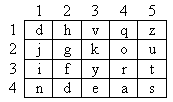
\includegraphics[width=4cm]{image/tab2d-vision-tab2d}
	\end{center}

	Ainsi, la valeur de \textstyleCodeInsr{tabLettres[3,4]} 
	est le caractère ‘r’. 
	
	La vision «~tableau de tableau~» 
	(ou décomposition en niveaux)
	donnerait :

	\begin{center}
	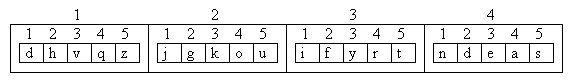
\includegraphics[width=0.9\textwidth]{image/tab2d-vision-tabtab}
	\end{center}

	Dans cette représentation, le tableau \textstyleCodeInsr{tabLettres} est
	d’abord décomposé à un premier niveau en quatre éléments auxquels on
	accède par le premier indice. Ensuite, chaque élément de premier niveau
	est décomposé en cinq éléments de deuxième niveau accessibles par le
	deuxième indice.
	
	\textbf{Exemple~:} reprenons l'exemple du stock de 10 produit
	\vref{tableau:tab1DStock10Articles} mais pour chaque jour de la semaine.
	
	
	\begin{center}
		\tablehead{}
		\begin{supertabular}{m{1.5cm}m{1.2cm}m{1.2cm}m{1.2cm}m{1.2cm}m{1.2cm}m{1.2cm}m{1.2cm}m{1.2cm}m{1.2cm}m{1.4cm}}
			~ &
			\centering  \textstyleCodeInsr{article1} &
			\centering  \textstyleCodeInsr{article2} &
			\centering  \textstyleCodeInsr{article3} &
			\centering  \textstyleCodeInsr{article4} &
			\centering  \textstyleCodeInsr{article5} &
			\centering  \textstyleCodeInsr{article6} &
			\centering  \textstyleCodeInsr{article7} &
			\centering  \textstyleCodeInsr{article8} &
			\centering  \textstyleCodeInsr{article9} &
			\centering\arraybslash 
			\textstyleCodeInsr{article10}\\\hhline{~----------}
			\multicolumn{1}{m{1.5cm}|}{\centering 
			\textstyleCodeInsr{lundi}} & 
			\multicolumn{1}{m{1.2cm}|}{cpt[1][1]} &
			\multicolumn{1}{m{1.2cm}|}{cpt[1][2]} &
			\multicolumn{1}{m{1.2cm}|}{cpt[1][3]} &
			\multicolumn{1}{m{1.2cm}|}{cpt[1][4]} &
			\multicolumn{1}{m{1.2cm}|}{cpt[1][5]} &
			\multicolumn{1}{m{1.2cm}|}{cpt[1][6]} &
			\multicolumn{1}{m{1.2cm}|}{cpt[1][7]} &
			\multicolumn{1}{m{1.2cm}|}{cpt[1][8]} &
			\multicolumn{1}{m{1.2cm}|}{cpt[1][9]} &
			\multicolumn{1}{m{1.4cm}|}{cpt[1][10]
			}\\\hhline{~----------}
			
			\multicolumn{1}{m{1.5cm}|}{\centering 
			\textstyleCodeInsr{mardi}} & 
			\multicolumn{1}{m{1.2cm}|}{cpt[2][1]} &
			\multicolumn{1}{m{1.2cm}|}{cpt[2][2]} &
			\multicolumn{1}{m{1.2cm}|}{cpt[2][3]} &
			\multicolumn{1}{m{1.2cm}|}{cpt[2][4]} &
			\multicolumn{1}{m{1.2cm}|}{cpt[2][5]} &
			\multicolumn{1}{m{1.2cm}|}{cpt[2][6]} &
			\multicolumn{1}{m{1.2cm}|}{cpt[2][7]} &
			\multicolumn{1}{m{1.2cm}|}{cpt[2][8]} &
			\multicolumn{1}{m{1.2cm}|}{cpt[2][9]} &
			\multicolumn{1}{m{1.4cm}|}{cpt[2][10]
			}\\\hhline{~----------}
			
			\multicolumn{1}{m{1.5cm}|}{\centering 
			\textstyleCodeInsr{mercredi}} & 
			\multicolumn{1}{m{1.2cm}|}{cpt[3][1]} &
			\multicolumn{1}{m{1.2cm}|}{cpt[3][2]} &
			\multicolumn{1}{m{1.2cm}|}{cpt[3][3]} &
			\multicolumn{1}{m{1.2cm}|}{cpt[3][4]} &
			\multicolumn{1}{m{1.2cm}|}{cpt[3][5]} &
			\multicolumn{1}{m{1.2cm}|}{cpt[3][6]} &
			\multicolumn{1}{m{1.2cm}|}{cpt[3][7]} &
			\multicolumn{1}{m{1.2cm}|}{cpt[3][8]} &
			\multicolumn{1}{m{1.2cm}|}{cpt[3][9]} &
			\multicolumn{1}{m{1.4cm}|}{cpt[3][10]
			}\\\hhline{~----------}
			
			\multicolumn{1}{m{1.5cm}|}{\centering 
			\textstyleCodeInsr{jeudi}} & 
			\multicolumn{1}{m{1.2cm}|}{cpt[4][1]} &
			\multicolumn{1}{m{1.2cm}|}{cpt[4][2]} &
			\multicolumn{1}{m{1.2cm}|}{cpt[4][3]} &
			\multicolumn{1}{m{1.2cm}|}{cpt[4][4]} &
			\multicolumn{1}{m{1.2cm}|}{cpt[4][5]} &
			\multicolumn{1}{m{1.2cm}|}{cpt[4][6]} &
			\multicolumn{1}{m{1.2cm}|}{cpt[4][7]} &
			\multicolumn{1}{m{1.2cm}|}{cpt[4][8]} &
			\multicolumn{1}{m{1.2cm}|}{cpt[4][9]} &
			\multicolumn{1}{m{1.4cm}|}{cpt[4][10]
			}\\\hhline{~----------}
			
			\multicolumn{1}{m{1.5cm}|}{\centering 
			\textstyleCodeInsr{vendredi}} & 
			\multicolumn{1}{m{1.2cm}|}{cpt[5][1]} &
			\multicolumn{1}{m{1.2cm}|}{cpt[5][2]} &
			\multicolumn{1}{m{1.2cm}|}{cpt[5][3]} &
			\multicolumn{1}{m{1.2cm}|}{cpt[5][4]} &
			\multicolumn{1}{m{1.2cm}|}{cpt[5][5]} &
			\multicolumn{1}{m{1.2cm}|}{cpt[5][6]} &
			\multicolumn{1}{m{1.2cm}|}{cpt[5][7]} &
			\multicolumn{1}{m{1.2cm}|}{cpt[5][8]} &
			\multicolumn{1}{m{1.2cm}|}{cpt[5][9]} &
			\multicolumn{1}{m{1.4cm}|}{cpt[5][10]
			}\\\hhline{~----------}
			
			\multicolumn{1}{m{1.5cm}|}{\centering 
			\textstyleCodeInsr{samedi}} & 
			\multicolumn{1}{m{1.2cm}|}{cpt[6][1]} &
			\multicolumn{1}{m{1.2cm}|}{cpt[6][2]} &
			\multicolumn{1}{m{1.2cm}|}{cpt[6][3]} &
			\multicolumn{1}{m{1.2cm}|}{cpt[6][4]} &
			\multicolumn{1}{m{1.2cm}|}{cpt[6][5]} &
			\multicolumn{1}{m{1.2cm}|}{cpt[6][6]} &
			\multicolumn{1}{m{1.2cm}|}{cpt[6][7]} &
			\multicolumn{1}{m{1.2cm}|}{cpt[6][8]} &
			\multicolumn{1}{m{1.2cm}|}{cpt[6][9]} &
			\multicolumn{1}{m{1.4cm}|}{cpt[6][10]
			}\\\hhline{~----------}
			
			\multicolumn{1}{m{1.5cm}|}{\centering 
			\textstyleCodeInsr{dimanche}} & 
			\multicolumn{1}{m{1.2cm}|}{cpt[7][1]} &
			\multicolumn{1}{m{1.2cm}|}{cpt[7][2]} &
			\multicolumn{1}{m{1.2cm}|}{cpt[7][3]} &
			\multicolumn{1}{m{1.2cm}|}{cpt[7][4]} &
			\multicolumn{1}{m{1.2cm}|}{cpt[7][5]} &
			\multicolumn{1}{m{1.2cm}|}{cpt[7][6]} &
			\multicolumn{1}{m{1.2cm}|}{cpt[7][7]} &
			\multicolumn{1}{m{1.2cm}|}{cpt[7][8]} &
			\multicolumn{1}{m{1.2cm}|}{cpt[7][9]} &
			\multicolumn{1}{m{1.4cm}|}{cpt[7][10]
			}\\\hhline{~----------}
		\end{supertabular}
	\end{center}
	
	\bigskip

	\cadre{
	\begin{pseudo}
	\LComment Calcule et affiche la quantité vendue de 10 produits
	\LComment pour chaque jour de la semaine (de 1~: lundi à 7~: dimanche).
	\Module{statistiquesVentesSemaine}{}{}
		\Empty
		\Decl cpt~: \K{tableau} [1 à 7, 1 à 10] d’entiers
		\Decl produit, jour~: entiers
		\Empty
		\Stmt initialiser(cpt)
		\Empty
		\LComment Pour chaque jour de la semaine
		\For{jour \K{de} 1 \K{à} 7}
			\Stmt traiterStock1Jour(cpt, jour)
			\For{produit \K{de} 1 \K{à} 10}
				\Write "quantité vendue de produit ", produit, " ce jour ", jour, "~: ", cpt[jour][i]
			\EndFor
		\EndFor	
	\EndModule
	\end{pseudo}
	}
	
	\cadre{
	\begin{pseudo}
	\LComment Ce module initialise le tableau d'entiers à 0
	\Module{initialiser}{entiers\InOut~: \K{tableau} [1 à 7, 1 à 10] d’entiers}{}
		\Decl i, j~: entiers
		\For{i \K{de} 1 \K{à} 7}
			\For{j \K{de} 1 \K{à} 10}
				\Let cpt[i][j] \Gets 0
			\EndFor
		\EndFor
	\EndModule
	\end{pseudo}
	}
	
	\cadre{
	\begin{pseudo}
	\LComment Ce module effectue le traitement du stock pour une journée.
	\Module{traiterStock1Jour}{cpt~\InOut: \K{tableau} [1 à 7, 1 à 10] d’entiers, jour~: entier}{}
		\Decl numéroProduit, quantité~: entiers
		\Write "Introduisez le numéro du produit~:"
		\Read numéroProduit
		\Empty
		\While{numéroProduit > 0}
			\Empty
			\Write "Introduisez la quantité vendue~:"
			\Read quantité
			\Empty
			\Let cpt[jour][numéroProduit] \Gets cpt[jour][numéroProduit] + quantité
			\Empty
			\Write "Introduisez le numéro du produit~:"
			\Read numéroProduit
			\Empty
		\EndWhile
	\EndModule
	\end{pseudo}
	}
	
	Pour plus d'exemples, allez faire un tour à l'\vref{algo:Tab2D}

% ============================================
\section{La troisième dimension (et au-delà)}
% ============================================

	Certaines situations complexes nécessitent l'usage de
	tableaux à 3 voire plus de dimensions.

	\marginicon{definition}
	Pour déclarer un tableau statique à $k$ dimensions, on écrira :

	\cadre{
	\begin{pseudo}
	\Decl nomTableau : \K{tableau} [ bMin\_1 à bMax\_1, \dots, bMin\_k à bMax\_k] de TypeElément
	\end{pseudo}
	}

	où chaque paire de bornes \textstyleCodeInsr{bMin\_i}~et
	\textstyleCodeInsr{bMax\_i} limite l’indice correspondant 
	à la $i^{ème}$	dimension du tableau.
	
	
% ================================================
\section{Parcours d'un tableau à deux dimensions}
%\label{algo:Tab2D}
% ================================================

Comme nous l'avons fait pour les tableaux à  une dimension,
envisageons le parcours des tableaux à deux dimensions 
(n lignes et m colonnes).

Déclaration d'un tableau statique~:

\cadre{
\begin{pseudo}
	\Decl tab~: tableau [1 à n, 1 à m] de T
\end{pseudo}
}

Déclaration d'un tableau dynamique~:

\cadre{
	\begin{pseudo}
	\Decl tab~: \K{tableau} de T
	\Let tab \Gets \K{nouveau} \K{tableau} [1 à n, 1 à m] de T
	\end{pseudo}
	}

Commençons par des cas plus simples 
où on ne parcourt qu'une seule des dimensions 
puis attaquons le cas général.

\subsection{Parcours d'une dimension}

On peut vouloir ne parcourir qu'une seule ligne du tableau.
Si on parcourt la ligne $l$, on visite les cases 
$(l,1)$, $(l,2)$, \dots, $(l,m)$.
L'indice de ligne est constant et c'est l'indice de colonne qui varie.

\begin{center}
$l$
\begin{tabular}{|*{5}{>{\centering\arraybackslash}m{0.3cm}|}}
\hline
\ & \ & \ & \ & \  \\
\hline
\cellcolor{gray!25}\ & \cellcolor{gray!25}\ & \cellcolor{gray!25}\ & \cellcolor{gray!25}\ & \cellcolor{gray!25}\  \\
\hline
\ & \ & \ & \ & \  \\
\hline
\end{tabular}
\end{center}

Ce qui donne l'algorithme :

\cadre{
\begin{pseudo}
	\LComment{Parcours de la ligne $l$ d'un tableau à deux dimensions}
	\For{c de 1 à m}
		\Stmt traiter tab[l,c]
	\EndFor
\end{pseudo}
}

Retenons~: pour parcourir une ligne, on utilise une boucle sur les colonnes. 

Symétriquement, on pourrait considérer le parcours de la colonne $c$
comme avec l'algorithme suivant.

\cadre{
\begin{pseudo}
	\LComment{Parcours de la colonne $c$ d'un tableau à deux dimensions}
	\For{l de 1 à n}
		\Stmt traiter tab[l,c]
	\EndFor
\end{pseudo}
}

Si le tableau est carré ($n=m$) on peut aussi envisager le parcours
des deux diagonales.

Pour la colonne descendante, 
les éléments à visiter sont $(1,1)$, $(2,2)$, \dots, $(n,n)$.

\begin{center}
\begin{tabular}{|*{3}{>{\centering\arraybackslash}m{0.3cm}|}}
\hline
\cellcolor{gray!25}\ & \ & \ \\
\hline
\ & \cellcolor{gray!25}\ & \ \\
\hline
\ & \ & \cellcolor{gray!25}\ \\
\hline
\end{tabular}
\end{center}

Une seule boucle suffit 
comme le montre l'algorithme suivant.

\cadre{
\begin{pseudo}
	\LComment{Parcours de la diagonale descendante d'un tableau carré}
	\For{i de 1 à n}
		\Stmt traiter tab[i,i]
	\EndFor
\end{pseudo}
}

Pour la colonne montante, 
on peut envisager deux solutions, 
avec deux indices ou un seul
en se basant sur le fait que $i+j=n+1 \Rightarrow j=n+1-i$.

\cadre{
\begin{pseudo}
	\LComment{Parcours de la diagonale montante d'un tableau carré - 2 indices}
	\Let j \Gets n
	\For{i de 1 à n}
		\Stmt traiter tab[i,j]
		\Let j \Gets j - 1
	\EndFor
\end{pseudo}
}

\cadre{
\begin{pseudo}
	\LComment{Parcours de la diagonale montante d'un tableau carré - 1 indice}
	\For{i de 1 à n}
		\Stmt traiter tab[i, n + 1 - i]
	\EndFor
\end{pseudo}
}

\subsection{Parcours des deux dimensions}

\subsubsection*{Parcours par lignes et par colonnes}

Les deux parcours les plus courants sont les parcours ligne par ligne
et colonne par colonne.
Les tableaux suivants montrent dans quel ordre chaque case est visitée dans ces deux parcours.

\begin{center}
\begin{minipage}{0.4\textwidth}
\begin{center}
Parcours ligne par ligne\\
\begin{tabular}{|*{5}{>{\centering\arraybackslash}m{0.35cm}|}}
\hline
1 & 2 & 3 & 4 & 5 \\
\hline
6 & 7 & 8 & 9 & 10 \\
\hline
11 & 12 & 13 & 14 & 15 \\
\hline
\end{tabular}
\end{center}
\end{minipage}
\qquad
\begin{minipage}{0.4\textwidth}
\begin{center}
Parcours colonne par colonne\\
\begin{tabular}{|*{5}{>{\centering\arraybackslash}m{0.35cm}|}}
\hline
1 & 4 & 7 & 10 & 13 \\
\hline
2 & 5 & 8 & 11 & 14 \\
\hline
3 & 6 & 9 & 12 & 15 \\
\hline
\end{tabular}
\end{center}
\end{minipage}
\end{center}

Le plus simple est d'utiliser deux boucles imbriquées 

\cadre{
\begin{pseudo}
	\LComment{Parcours d'un tableau à 2 dimensions, ligne par ligne}
	\For{lg de 1 à n}
		\For{col de 1 à m}
			\Stmt traiter tab[lg,col]
		\EndFor
	\EndFor
\end{pseudo}
}

\cadre{
\begin{pseudo}
	\LComment{Parcours d'un tableau à 2 dimensions, colonne par colonne}
	\For{col de 1 à m}
		\For{lg de 1 à n}
			\Stmt traiter tab[lg,col]
		\EndFor
	\EndFor
\end{pseudo}
}

Mais on peut obtenir le même résultat avec une seule boucle
si l'indice sert juste à compter le nombre de passages
et que les indices de lignes et de colonnes sont gérés manuellement.

L'algorithme suivant montre ce que ça donne
pour un parcours ligne par ligne.
La solution pour un parcours colonne par colonne est similaire
et laissée en exercice.

\cadre{
\begin{pseudo}
	\LComment{Parcours d'un tableau à 2 dimensions via une seule boucle}
	\Let lg \Gets 1
	\Let col \Gets 1
	\For{i de 1 à n*m}
		\Stmt traiter tab[lg,col]
		\Let col \Gets col + 1	\RComment Passer à la case suivante
		\If{col > m} \RComment On déborde sur la droite, passer à la ligne suivante
			\Let col \Gets 1
			\Let lg \Gets lg + 1
		\EndIf
	\EndFor
\end{pseudo}
}

L'avantage de cette solution apparaitra 
quand on verra des situations plus difficiles.

\subsubsection*{Interrompre le parcours}

Comme avec les tableaux à une dimension, 
envisageons l'arrêt prématuré lors de la rencontre d'une certaine condition.
Et, comme avec les tableaux à une dimension, 
transformons d'abord nos \K{pour} en \K{tant que}.

Par exemple, montrons les deux parcours ligne par ligne, avec une et deux boucle(s).

\cadre{
\begin{pseudo}
	\LComment{Parcours d'un tableau à 2 dimensions, ligne par ligne, via un tant que}
	\Let lg \Gets 1
	\While{lg < n}
		\Let col \Gets 1
		\While{col < m}
			\Stmt traiter tab[lg, col]
			\Let col \Gets col + 1
		\EndWhile
		\Let lg \Gets lg + 1
	\EndWhile
\end{pseudo}
}

\cadre{
\begin{pseudo}
	\LComment{Parcours d'un tableau à 2 dimensions via une seule boucle et un tant que}
	\Let lg \Gets 1
	\Let col \Gets 1
	\Let i \Gets 1
	\While{i $\le$ n*m} \RComment ou "lg $\le$ n" 
		\Stmt traiter tab[lg,col]
		\Let col \Gets col + 1	\RComment Passer à la case suivante
		\If{col > m} \RComment On déborde sur la droite, passer à la ligne suivante
			\Let col \Gets 1
			\Let lg \Gets lg + 1
		\EndIf
		\Let i \Gets i + 1		
	\EndWhile
\end{pseudo}
}

On peut à présent introduire le test comme on l'a fait 
dans les algorithmes de parcours des tableaux à une dimension.

Illustrons-le au travers de deux exemples.
Le premier introduit un test en utilisant un booléen
alors que le second introduit un test
sans utiliser de booléen.

\cadre{
\begin{pseudo}
	\LComment{Parcours avec test d'arrêt - deux boucles et un booléen}
	\Let trouvé \Gets faux
	\Let lg \Gets 1
	\While{lg $<$ n ET NON trouvé}
		\Let col \Gets 1
		\While{col $<$ m ET NON trouvé}
			\If{\textit{tab[lg, col] impose l'arrêt du parcours}}
				\Let trouvé \Gets vrai
			\Else \RComment Ne pas modifier les indices si arrêt demandé
				\Let col \Gets col + 1
			\EndIf
		\EndWhile
		\If{NON trouvé} \RComment Ne pas modifier les indices si arrêt demandé
			\Let lg \Gets lg + 1
		\EndIf
	\EndWhile
\end{pseudo}
}

\cadre{
\begin{pseudo}
	\LComment{Parcours avec test d'arrêt - une boucle et pas de booléen}
	\Let lg \Gets 1
	\Let col \Gets 1
	\Let i \Gets 1
	\While{i $\le$ n*m ET \textit{tab[lg, col] n'impose pas l'arrêt}}  
		\Let col \Gets col + 1	\RComment Passer à la case suivante
		\If{col > m} \RComment On déborde sur la droite, passer à la ligne suivante
			\Let col \Gets 1
			\Let lg \Gets lg + 1
		\EndIf
		\Let i \Gets i + 1		
	\EndWhile
	\LComment Arrêt prématuré si i $\le$ n*m.
\end{pseudo}
}

\subsubsection*{Parcours plus compliqué - le serpent}

Envisageons un parcours plus difficile illustré par le tableau suivant.

\begin{center}
\begin{tabular}{|*{5}{>{\centering\arraybackslash}m{0.35cm}|}}
\hline
1 & 2 & 3 & 4 & 5 \\
\hline
10 & 9 & 8 & 7 & 6 \\
\hline
11 & 12 & 13 & 14 & 15 \\
\hline
\end{tabular}
\end{center}

Le plus simple est d'adapter l'algorithme de parcours 
avec une seule boucle
en introduisant un sens de déplacement, 
ce qui donne l'algorithme :

\cadre{
\begin{pseudo}
	\LComment{Parcours du serpent dans un tableau à deux dimensions}
	\Let lg \Gets 1
	\Let col \Gets 1
	\Let depl \Gets 1	\RComment 1 pour avancer, -1 pour reculer
	\For{i de 1 à n*m}
		\Stmt traiter tab[lg, col]
		\If{1 $\le$ col + depl ET col + depl $\le$ m}
			\Let col \Gets col + depl \RComment On se déplace dans la ligne
		\Else
			\Let lg \Gets lg + 1	\RComment On passe à la ligne suivante
			\Let depl \Gets -depl	\RComment et on change de sens
		\EndIf
	\EndFor
\end{pseudo}
}


% ===================
\section{ Exercices}
% ===================

\begin{Exercice}{Affichage}
	Écrire un module qui affiche tous les éléments d'un
	tableau à $n$ lignes et $m$ colonnes
	\begin{enumerate}[label=\alph*)]
	\item ligne par ligne ;
	\item colonne par colonne.
	\end{enumerate}
\end{Exercice}

\begin{Exercice}{Les nuls}
	\marginicon{java}
	Écrire un module qui reçoit un tableau ($n$ x $m$)
	d'entiers et qui affiche la proportion
	d'éléments nuls dans ce tableau.
\end{Exercice}

\begin{Exercice}{Le contour du tableau}
	\marginicon{java}
	On donne un tableau d’entiers \code{tabEnt} 
	à $n$ lignes et $m$ colonnes. 
	Écrire un module retournant la somme 
	de tous les éléments \textit{impairs}
	situés sur le bord du tableau.

	Exemple : pour le tableau suivant, le module doit renvoyer $32$

	\begin{center}
	\begin{tabular}{|*{4}{>{\centering\arraybackslash}m{0.6cm}|}}
	  \hline
	  3 & 4 & 6 & 11\\\hline
	  2 & 21 & 7 & 9\\\hline
	  1 & 5 & 12 & 3\\\hline
	\end{tabular}
	\end{center}

	Et pour le suivant, le module doit renvoyer $6$

	\begin{center}
	\begin{tabular}{|*{5}{>{\centering\arraybackslash}m{0.3cm}|}}
	\hline
	 4 & 1 & 2 & 8 & 5\\\hline
	\end{tabular}
	\end{center}
\end{Exercice}

\begin{Exercice}{À vos pinceaux !}
	On possède un tableau à $n$ lignes et $n$ colonnes dont les éléments de type
	Couleur valent NOIR ou BLANC. On suppose que le tableau est initialisé
	à ‘BLANC’ au départ. Écrire un module qui ‘noircit’ les cases de ce
	tableau comme le suggèrent les dessins suivants~(les exemples sont
	donnés pour un tableau 10 x 10 mais les algorithmes doivent fonctionner
	quelle que soit la taille du tableau).
	
	\begin{center}
	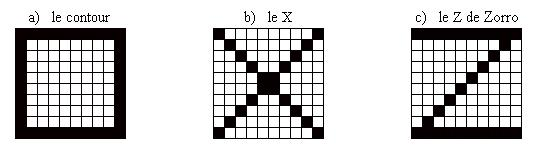
\includegraphics[width=0.9\textwidth]{image/tab2d-ex-oxz}
	\end{center}
\end{Exercice}

\begin{Exercice}{Le tableau de cotes}
	Soit un tableau à $n$ lignes et $m$ colonnes d'entiers où
	une ligne représente les notes sur 20 d'un étudiant et
	les colonnes toutes les notes d'un cours.
	
	Écrire un algorithme recevant ce tableau en paramètre et affichant le
	pourcentage d'étudiants ayant obtenu une moyenne
	supérieure à 50\%.
\end{Exercice}

\begin{Exercice}{Tous positifs}
	\marginicon{java}
	Écrire un module qui reçoit un tableau ($n$ x $m$) d’entiers et qui vérifie
	si tous les nombres qu’il contient sont strictement positifs. Bien sûr,
	on veillera à éviter tout travail inutile; la rencontre d’un nombre
	négatif doit arrêter le module.
\end{Exercice}

\begin{Exercice}{Le carré magique}
	\marginicon{java}
	Un carré magique est un tableau d’entiers carré
	(c'est-à-dire possédant autant de lignes que de
	colonnes) ayant la propriété suivante: si on additionne les éléments
	d'une quelconque de ses lignes, de ses colonnes ou de
	ses deux diagonales, on obtient à chaque fois le même résultat.

	Écrire un module recevant en paramètres le tableau [1 à $n$, 1 à $n$]
	d'entiers Carré et renvoyant une valeur booléenne
	indiquant si Carré est un carré magique ou non.
\end{Exercice}

\begin{Exercice}{Le triangle de Pascal}
	Le triangle de Pascal est construit de la façon suivante :

	\begin{liste}
	\item la ligne initiale contient un seul élément de valeur 1 ;
	\item chaque ligne possède un élément de plus que la précédente ;
	\item chaque ligne commence et se termine par 1 ;
	\item 
		pour calculer un nombre d’une autre case du tableau, on additionne le
		nombre situé dans la case située juste au-dessus avec celui dans la
		case à la gauche de la précédente.
	\end{liste}

	Écrire un module qui reçoit en paramètre un entier
	$n$, et qui renvoie un tableau contenant les
	$n+1$ premières lignes du triangle de Pascal
	(indicées de $0$ à $n$).
	
	N.B.: le «~triangle~» sera bien entendu renvoyé dans un tableau carré.
	Quid des cases non occupées ?

	Par exemple, pour $n$ qui vaut 5, on aura le tableau suivant :

	\begin{center}
	\begin{tabular}{|*{6}{>{\centering\arraybackslash}m{0.35cm}|}}
	\hline
	 1 & ~ & ~ & ~ & ~ & ~ \\\hline
	 1 & 1 & ~ & ~ & ~ & ~ \\\hline
	 1 & 2 & 1 & ~ & ~ & ~ \\\hline
	 1 & 3 & 3 & 1 & ~ & ~ \\\hline
	 1 & 4 & 6 & 4 & 1 & ~ \\\hline
	 1 & 5 & 10 & 10 & 5 & 1 \\\hline
	\end{tabular}
	\end{center}
\end{Exercice}

\begin{Exercice}{Le calendrier du mois}
	Écrire un module qui reçoit en paramètres 
	le numéro du premier jour du mois 
	(c-à-d 1 si le mois commence un lundi, 2 si le mois commence un mardi,
	etc.) ainsi que le nombre de jours dans le mois.
	Au départ de ces données, 
	le module remplira avec les dates des jours du mois un tableau
	«~calendrier~» à deux dimensions, 
	dont les colonnes représentent les jours 
	(la première colonne correspondant au lundi) et les lignes les
	semaines. 
	Par exemple, si le mois contient 30 jours et le premier jour
	est un mercredi, le contenu du tableau sera :

	\begin{center}
	\tablehead{}
	\begin{supertabular}{|m{0.807cm}|m{0.807cm}|m{0.807cm}|m{0.807cm}|m{0.807cm}|m{0.807cm}|m{0.81100005cm}|}
	\multicolumn{1}{m{0.807cm}}{\centering 
	\textstylePolicepardfauti{L}} &
	\multicolumn{1}{m{0.807cm}}{\centering 
	\textstylePolicepardfauti{M}} &
	\multicolumn{1}{m{0.807cm}}{\centering 
	\textstylePolicepardfauti{M}} &
	\multicolumn{1}{m{0.807cm}}{\centering 
	\textstylePolicepardfauti{{J}}} &
	\multicolumn{1}{m{0.807cm}}{\centering 
	\textstylePolicepardfauti{{V}}} &
	\multicolumn{1}{m{0.807cm}}{\centering 
	\textstylePolicepardfauti{{S}}} &
	\multicolumn{1}{m{0.81100005cm}}{\centering\arraybslash
	 \textstylePolicepardfauti{D}}\\\hline
	~
	 &
	~
	 &
	\raggedleft  \textstylePolicepardfauti{1} &
	\raggedleft  \textstylePolicepardfauti{2} &
	\raggedleft  \textstylePolicepardfauti{3} &
	\raggedleft  \textstylePolicepardfauti{4} &
	\raggedleft\arraybslash 
	\textstylePolicepardfauti{5}\\\hline
	\raggedleft  \textstylePolicepardfauti{6} &
	\raggedleft  \textstylePolicepardfauti{7} &
	\raggedleft  \textstylePolicepardfauti{8} &
	\raggedleft  \textstylePolicepardfauti{9} &
	\raggedleft  \textstylePolicepardfauti{10} &
	\raggedleft  \textstylePolicepardfauti{11} &
	\raggedleft\arraybslash 
	\textstylePolicepardfauti{12}\\\hline
	\raggedleft  \textstylePolicepardfauti{13} &
	\raggedleft  \textstylePolicepardfauti{14} &
	\raggedleft  \textstylePolicepardfauti{15} &
	\raggedleft  \textstylePolicepardfauti{16} &
	\raggedleft  \textstylePolicepardfauti{17} &
	\raggedleft  \textstylePolicepardfauti{18} &
	\raggedleft\arraybslash 
	\textstylePolicepardfauti{19}\\\hline
	\raggedleft  \textstylePolicepardfauti{20} &
	\raggedleft  \textstylePolicepardfauti{21} &
	\raggedleft  \textstylePolicepardfauti{22} &
	\raggedleft  \textstylePolicepardfauti{23} &
	\raggedleft  \textstylePolicepardfauti{24} &
	\raggedleft  \textstylePolicepardfauti{25} &
	\raggedleft\arraybslash 
	\textstylePolicepardfauti{26}\\\hline
	\raggedleft  \textstylePolicepardfauti{27} &
	\raggedleft  \textstylePolicepardfauti{28} &
	\raggedleft  \textstylePolicepardfauti{29} &
	\raggedleft  \textstylePolicepardfauti{30} &
	~
	 &
	~
	 &
	~
	\\\hline
	\end{supertabular}
	\end{center}

	\textbf{Réflexions} :

	\begin{liste}
	\item Combien de lignes au maximum doit avoir ce tableau ?
	\item Quid des cases non occupées ?
	\end{liste}
\end{Exercice}

\begin{Exercice}{À vos pinceaux (la suite) !}
	Pour poursuivre l'exercice du pinceau, 
	voici quelques cas plus coriaces.
	
	\begin{center}
	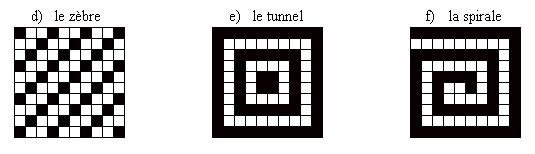
\includegraphics[width=0.9\textwidth]{image/tab2d-ex-zts}
	\end{center}
\end{Exercice}

\begin{Exercice}{Exercices sur la complexité}

	Quelle est la complexité 
	\begin{enumerate}[label=\alph*)]
	\item 
		d’un algorithme de parcours	d'un tableau $n$ x $n$ ?
	\item
		d'un algorithme qui remet à 0 toutes les
		occurrences du maximum d'un tableau $n$ x $n$ ?
	\item 
		de l'algorithme que vous avez écrit pour résoudre les
		exercices du pinceau ?
	\end{enumerate}
\end{Exercice}

\begin{Exercice}{Lignes et colonnes}
	Écrire un module qui reçoit un tableau d’entiers à 2 dimensions en paramètre 
	et qui retourne un booléen indiquant si ce tableau 
	possède 2 lignes ou 2 colonnes identiques.
	
	Dans l’affirmative, 
	ce module renverra également en paramètres les informations suivantes :
	
	\begin{liste}
	\item les indices des lignes ou colonnes identiques
	\item un caractère valant ‘L’ ou ‘C’ selon qu’il s’agit de lignes ou de
	colonnes
	\end{liste}
	
	Dans la négative, les valeurs de ces paramètres seront indéterminées ou
	quelconques, elles ne seront de toute façon pas utilisées par le module
	appelant.
\end{Exercice}

%========================
\chapter{L'orienté objet}
%=========================


	\marginicon{objectif}
		Dans ce chapitre, nous présentons les bases de la programmation orientée
		objet. Nous commençons par expliquer les motivations qui ont amené ce
		type de programmation avant d'entrer dans le vif du
		sujet en explicitant le concept
		d'\textit{encapsulation}. Les autres piliers de
		l'orienté objet (\textit{héritage} et
		\textit{polymorphisme}) ne seront pas vus cette année.


%===================
\section{Motivation}
%====================

	Depuis son apparition, la puissance de l'ordinateur
	n'a cessé de croitre exponentiellement. Les tâches qui
	lui sont confiées ont fait de même. Ainsi les programmes à écrire sont
	de plus en plus gros et de plus en plus complexes.
	
	Face à la complexité, la démarche est toujours la même : découper le
	problème en sous-problèmes (qui peuvent à leur tour être découpés) ce
	qui permet

	\liststyleListv
	\begin{itemize}
		\item 
			d'attaquer chaque problème séparément en évitant la
			surcharge cognitive ;
		\item 
			de répartir le travail entre plusieurs personnes ;
		\item 
			de pouvoir réutiliser du travail déjà produit si un sous-problème est
			déjà apparu dans le cadre d'un autre problème ;
		\item 
				de produire un code plus lisible car s'exprimant avec
				des termes de plus haut niveau, plus proches du problème à résoudre.
				Ainsi, là où un tri devra être fait, on trouvera le mot «~trier~» qui
				fera référence à la partie de code qui s’occupe du tri. Cela va dans le
				sens d’une plus grande «~abstraction~» du code : un code qui s’éloigne
				du langage simpliste compris par le processeur pour s’approcher de la
				pensée humaine et des termes du problème à résoudre.
	\end{itemize}
	
	Les langages de programmation ont suivi cette approche en permettant
	toujours plus d’abstraction. Dans un chapitre précédent, on vous a
	présenté la notion de module qui permet de découper la tâche à réaliser
	en sous-tâches ainsi que la notion de structure qui permet de regrouper
	des données. Il s'agit là de deux approches	dissociées. 

	C'est cette lacune que se propose de combler
	l'orienté objet : permettre de définir des
	\textbf{objets} (composés de \textbf{données} et
	\textbf{d'instructions}) qui sont proches du problème
	à résoudre. Cela va permettre une meilleure lisibilité et une plus
	grande concision du code. Ainsi on pourra définir les notions de date,
	d'employé, de fournisseur, de plateau de jeu, de pion,
	de livre, d'emprunteur, de carte à jouer, de chambre,
	de réservation, de vol, de produit, de stock, de ristourne, de facture,
	de panier d'achats, de compte en banque, de banque, de
	client, de portefeuille d'actions, ...


%==========================
\section{La notion d'objet}
%==========================

\marginicon{definition}
{\sffamily\bfseries\upshape
Définition\footnote{Les définitions sont tirées du livre de Cardon et
Dabancourt (cf. bibliographie)}}

Un \textbf{objet} est une entité logicielle qui :

\liststyleListi
\begin{itemize}
	\item 
		a une \textbf{identité~}; c'est-à-dire que nous pouvons
		identifier un objet par un nom (tout comme une variable possède un
		nom).
	\item 
		est capable de sauvegarder un \textbf{état}, c'est à
		dire un ensemble d'informations dans des variables
		internes;
	\item 
		répond à des \textbf{messages} précis en déclenchant des activations
		internes appropriées qui peuvent changer l'état de
		l'objet. Ces opérations sont appelées des
		\textbf{méthodes}. Ce sont des fonctions liées à des objets et qui
		précisent le \textbf{comportement} de ces objets.
\end{itemize}

{\sffamily\bfseries\upshape
État}

Un objet contient de l'information, des données qui
définissent son état.

{\bfseries
Exemples}

\liststyleListv
\begin{itemize}
	\item 
		Pour un produit, l'état peut être :
		l'intitulé du produit, son code barre, son prix, ... 
	\item 
		Pour un employé, on peut avoir : son nom, son prénom, son adresse, sa
		date d'embauche, son salaire mensuel, sa fonction, son
		téléphone, ... 
	\item 
		Une carte à jouer a une couleur et une valeur.
	\item 
		L'état d'une date est le jour du
		calendrier qu'elle représente.
	\item 
		L'état d'une heure est le moment de la
		journée qu'elle représente.
\end{itemize}

L'état d'un objet est mémorisé via des
variables qu'on appelle des \textit{attributs}.

\bigskip

\marginicon{definition}
{\sffamily\bfseries\upshape
Attributs}

Les \textbf{attributs} d'un objet sont
l'ensemble des informations se présentant sous forme
de variables et permettant de représenter l'état
d'un objet.

Nous verrons plus loin la syntaxe précise pour définir les attributs
d'un objet.

{
\textbf{Exemples} }

\liststyleListv
\begin{itemize}
	\item 
		L'intitulé d'un produit peut être
		représenté par une chaine. C'est également le cas des
		nom et prénom(s) d'un employé.
	\item 
		La date d'embauche peut être représentée par un «~objet
		date~» (une date est rarement un type primitif du langage utilisé). Un
		attribut d'un objet peut être lui même un objet.
	\item 
		Un moment de la journée peut aussi être un objet représenté par trois
		entiers\footnote{Toutefois, on verra que ce n'est
		peut-être pas la meilleure solution.} : les heures, les minutes et les
		secondes (en supposant qu'on désire une précision de
		l'ordre de la seconde).
	\item 
		L'adresse d'un employé peut être
		représentée par une seule chaine mais également par un «~objet
		adresse~» (qui contiendrait : une rue, un numéro, un code postal,
		...).
\end{itemize}

\marginicon{attention}
{\textbf{Remarque}\textbf{ : }Certaines parties de
l'état peuvent évoluer au fil du temps.
D'autres parties sont immuables. Ainsi
l'adresse d'une personne peut changer
mais pas sa date de naissance. }

\marginicon{exercice}
{\sffamily\bfseries\scshape
Exercices - attributs}

\liststyleWWviiiNumi
\begin{enumerate}
	\item 
		Quel(s) attribut(s) prendriez-vous pour représenter
		(l'état d') une date ?
	\item 
		Et pour un étudiant ?
	\item 
		Et pour un dé à 6 faces ?
	\item 
		Et pour une télévision ? \ (on peut en trouver vraiment beaucoup !)
\end{enumerate}

\bigskip

\marginicon{definition}
{\sffamily\bfseries\upshape
Comportement}

{Le \textbf{comportement} d'un objet est défini par
l'ensemble des messages ou requêtes auxquels il peut
répondre.}

Pour ce faire, il exécute une fonction (un module) qui pourra
éventuellement retourner une information à l'émetteur
du message.

Les messages peuvent interroger l'objet, le modifier,
lui demander d'agir sur son environnement (afficher du
texte, modifier un fichier, ...). 

{
\textbf{Exemples} }

\liststyleListv
\begin{itemize}
	\item {
		Quels «~messages~» peut-on envoyer à une date ? On peut lui demander
		(entre autres):}
			\begin{itemize}
				\item {
					des informations sur le jour du mois, le mois, l'année,
					le jour de la semaine ; }
				\item {
					si elle est antérieure ou non à une autre date ;}
				\item {
					si elle fait partie d'une année bissextile ; }
				\item {
					le nombre de jours qui la sépare de la fin de l'année
					;}
				\item {
					de passer au jour suivant, à la semaine suivante, ...}
			\end{itemize}
	\item 
		Et pour un stock de produits ? On peut 
		\begin{itemize}
			\item {
				lui demander la quantité disponible d'un produit donné
				;}
			\item {
				lui annoncer l'arrivée d'une quantité
				donnée d'un produit donné ;}
			\item {
				lui indiquer qu'un produit n'existe
				plus (à retirer du stock) ;}
			\item {
				lui demander d'enlever une certaine quantité
				d'un produit du stock.}
		\end{itemize}
	\item {
		Et pour un employé ? On peut}
		\begin{itemize}
			\item {
				lui demander son adresse, son salaire ou sa fonction, ...}
			\item {
				augmenter son salaire ;}
			\item {
				le changer de fonction ;}
			\item {
				le licencier (penser à prévoir une date de départ dans
				l'état !).}
		\end{itemize}
	\item {
		Pour un moment de la journée on peut demander s'il se
		situe le matin ou pas, ...}	
\end{itemize}

\marginicon{exercice}
{\sffamily\bfseries\scshape
Exercice - comportement}

\begin{enumerate}
	\item {
		Quel comportement voyez-vous pour un téléviseur ?}
	\item {
		Et pour un étudiant ?}
\end{enumerate}

\bigskip

\marginicon{definition}
{\sffamily\bfseries\upshape
Méthode}

{Un message lance l'exécution d'un
module appelé \textbf{méthode} dans le jargon de
l'orienté objet. }

{\bfseries
Exemples}

\liststyleListv
\begin{itemize}
	\item {
		Pour permettre à une date de passer au jour suivant, nous allons définir
		un méthode qui incrémente le jour du mois en tenant compte
		d'un possible basculement au mois suivant ou à
		l'année suivante.}
	\item {
		Pour permettre à un moment d'indiquer
		s'il est le matin ou pas, nous allons définir une
		méthode comme celle-ci \ (nous verrons plus tard comment
		l'associer aux objets)}

		\bigskip

		\cadre{
		\begin{pseudo}
			\LComment On suppose que 'heure' est un des attributs utilisés
			\LComment pour représenter l'état (le moment dans la journée)
			\Method{estMatin}{}{booléen}
				\Return heure > 12 // on considère
				que midi est situé l'après-midi
			\EndMethod
		\end{pseudo}
		}
		\\
		\bigskip
		{
		Cet exemple devrait vous sembler familier à deux exceptions près}

		\liststyleListv
		\begin{itemize}
			\item {
				on utilise le mot «~\textstyleMotCl{méthode}~» en lieu et place de
				«~\textstyleMotCl{module}~» ;}
			\item {
				les attributs (l'heure ici) ne sont pas passés en
				paramètre. Un objet connait déjà son état et donc la valeur de ses
				attributs. Nous verrons plus loin la syntaxe précise.}
	\end{itemize}
\end{itemize}

\marginicon{exercice}
{\sffamily\bfseries\scshape
Exercices - méthodes}

\liststyleWWviiiNumi
\begin{enumerate}
	\item 
		Dans le comportement d'un téléviseur, on retrouve
		«~éteindre~» et «~allumer~». À quoi ressemblerait le code de ces
		méthodes ?
	\item 
		Écrivez la méthode qui permet de passer au jour suivant.
\end{enumerate}

\bigskip

{\sffamily\bfseries
Activer un comportement}

{
Pour activer un comportement d'un objet, il faut lui
envoyer un message (ou dit autrement, appeler une de ses méthodes). La
syntaxe que nous allons utiliser (c'est la plus
courante) est la notation pointée}

\cadre{
\begin{pseudo}
	\Stmt nomObjet.nomMéthode()
\end{pseudo}
}

{\bfseries
Exemple}

{
Supposons que le nom «~maintenant~» désigne un objet contenant un moment
de la journée (on verra comment réaliser cela). Si on veut savoir si on
est le matin, on peut écrire}

\cadre{
\begin{pseudo}
	\If{maintenant.estMatin()}
		\Stmt ...
	\EndIf
\end{pseudo}
}


\bigskip

\marginicon{exercice}
{\sffamily\bfseries\scshape
Exercice – activer un comportement}

Écrire la portion de code qui allume une télévision (désignée par
«~maTélévision~») et puis l'éteint aussitôt après.


\bigskip

{\sffamily\bfseries\upshape
Les paramètres d'un comportement}

{
Activer un comportement revient à appeler une méthode de
l'objet. Souvent il est nécessaire
d'envoyer à l'objet des informations
complémentaires pour préciser notre demande ce qui se fait via
l'utilisation des paramètres.}

{\bfseries
Exemple}

Si on veut modifier le salaire d'un employé, il faut
que notre message contienne le nouveau salaire. Autrement dit, il faut
communiquer ce nouveau salaire à la méthode de changement du salaire.
Ce qui donne la méthode suivante :

\cadre{
\begin{pseudo}
	\Method{modifierSalaire}{nouveauSalaire : entier}{}
		\Stmt salaire \Gets nouveauSalaire
	\EndMethod
\end{pseudo}
}

\bigskip

\marginicon{exercice}
{\sffamily\bfseries\scshape
Exercices – paramètres du comportement}

\liststyleWWviiiNumi
\begin{enumerate}
	\item 
		Prenons un objet représentant un étudiant. 
		Nous supposerons qu'un étudiant a un \textit{numéro}, un 
		\textit{nom}, une \textit{annéeÉtude}, est ou non 
		\textit{doubleur} et est ou non \textit{ancien}
		Donnez les entêtes des méthodes suivantes qui permettent de
		:

		\liststyleListv
		\begin{itemize}
			\item 
				demander le numéro d'un étudiant
			\item 
				demander si un étudiant est doubleur ou non
			\item 
				modifier l'année détude d'un étudiant
			\item 
				faire réussir un étudiant
			\item 
				faire rater un étudiant.
		\end{itemize}
			
	\item 
		Prenons un objet représentant une date du calendrier grégorien. 
		Donnez les entêtes des méthodes suivantes qui permettent de
		:

		\liststyleListv
		\begin{itemize}
			\item
				demander le jour de la semaine d'une date
			\item 
				savoir si une date est antérieure ou non à une autre
			\item 
				connaitre le nombre de jours (absolu) séparant deux dates.
		\end{itemize}
		
	\item 
		Utilisation. Soit «~date1~» et «~date2~», deux dates ; écrivez la
		portion de code qui utilise les méthodes ci-dessus pour
		
		\liststyleListv
		\begin{itemize}
			\item 
				vérifier quelle date précède l'autre;
			\item 
				calculer le nombre de jours d'écart entre ces deux
				dates.
		\end{itemize}
	
	\item 
		Précédemment, vous avez défini l'ensemble du
		comportement d'un téléviseur. Écrivez les entêtes des
		méthodes correspondant à ce comportement ainsi qu'une
		portion de code qui les utilise.
\end{enumerate}

\bigskip


%=========================
\section{L'encapsulation}
%=========================

Un objet possède un état qui est représenté par des attributs. Les
bonnes pratiques de la programmation orientée objet préconisent
fortement que les attributs d'un objet soient
invisibles en dehors de l'objet. Ils ne pourront être
accédés qu'au travers du comportement de
l'objet, c'est-à-dire via ses
méthodes.

\marginicon{definition}
{\sffamily\bfseries\upshape
{
Lorsque les détails de l'implémentation
d'un objet sont masqués aux autres objets, on dit
qu'il y a \textbf{encapsulation} des données et du
comportement des objets.}}


Pourquoi une telle recommandation ? Le but est de garantir la cohérence
de l'état de l'objet. Si on pouvait
accéder directement à un attribut (et donc le modifier), on pourrait y
mettre une valeur incohérente. Par exemple, on pourrait dire que les
minutes d'un moment valent -3 ou 75 ou encore que le
jour de la date est 32 !

Dès lors, il nous faudra préciser pour chaque \textbf{membre} (attributs
et méthodes) d'un objet s'il est
\textbf{privé} (inconnu de l'extérieur) ou
\textbf{public} (connu de l'extérieur). 

Le bon usage impose que tous les attributs soient rendus privés et que
les méthodes restent publiques. Toutefois, on pourra trouver également
des méthodes privées. Ce sera notamment le cas si plusieurs méthodes
d'un objet ont une partie commune; \ il sera
intéressant de la \textit{factoriser}, c-à-d en faire une méthode
privée (ex : un calcul de maximum).

Puisqu'un attribut est privé, il est courant pour
chacun des attributs de rencontrer une méthode destinée à connaitre la
valeur de cet attribut et une autre qui permet de la modifier.

{\sffamily\bfseries\upshape
Accesseur et mutateur}

\marginicon{definition}
{\sffamily\bfseries\upshape
{
\textbf{Accesseur}\footnote{\textstyleFootnoteSymbol{On utilise aussi
souvent le mot anglais «~getter~». }} : méthode dont le but est de
fournir la valeur d'un attribut
\textbf{Mutateur}\footnote{\textstyleFootnoteSymbol{On utilise aussi
souvent le mot anglais «~setter~»}} : méthode dont le but est de
modifier la valeur d'un attribut}}

Par convention, ces méthodes sont nommées «~getNom~» et «~setNom~» où
«~nom~» est le nom de
l'attribut\footnote{\textstyleFootnoteSymbol{Pour un
attribut booléen, on pourra préférer «~estNom~» au lieu de
«~getNom~»}}. Par facilité, on utilisera parfois le terme «~accesseur~»
pour désigner à la fois les «~accesseurs~» et les «~mutateurs~».

{\bfseries
Exemple}

Écrivons l'accesseur et le mutateur pour
l'attribut «~heure~» d'un moment de
la journée

\cadre{
\begin{pseudo}
	\Method{getHeure}{}{entier}
		\Return heure
	\EndMethod
\end{pseudo}
}

\bigskip

\cadre{
\begin{pseudo}
	\Method{setHeure}{uneHeure : entier}{}
		\Stmt heure \Gets uneHeure
	\EndMethod
\end{pseudo}
}

\bigskip

{\sffamily\bfseries\upshape
Que faire si le paramètre est invalide ? }

Dans l'exemple précédent, que se passerait-il si le
paramètre \textstyleCodeInsr{uneHeure} vaut 25 ? Une valeur aberrante sera
affectée à l'attribut \textstyleCodeInsr{heure}.

Dans le cas de paramètres invalides, la plus mauvaise solution est de ne
rien faire. Le programme continuerait en croyant que tout s’est bien
passé et il court à la catastrophe. Il est préférable qu’un programme
se plante plutôt que de fournir une mauvaise réponse. 

Dans certains langages (comme le C), l’usage est que chaque module
retourne un entier indiquant s'il y a eu une erreur
(et laquelle). L’inconvénient est que le module appelant n’est pas
obligé de tenir compte de l’erreur.

Les \textbf{exceptions} sont un mécanisme du même genre mais qui oblige
à fournir un code de traitement de l’erreur. Il ne sera pas étudié en
première année\footnote{\textstyleFootnoteSymbol{En tout cas pas au
cours de Logique mais vous étudierez cette notion au cours de Java.}}.

Cette année, nous nous contenterons d'indiquer
clairement dans nos codes qu'il
s'agit d'une situation anormale via
la primitive \textstyleMotCl{erreur} qui arrête le déroulement du
programme avec une courte explication du problème.

La syntaxe que nous allons retenir est

\cadre{
\begin{pseudo}
	\Stmt \K{erreur} "explication de l'erreur"
\end{pseudo}
}

\bigskip

Ce qui donne :

\cadre{
\begin{pseudo}
	\Method{setHeure}{uneHeure : entier}{}
		\If{uneHeure < 0 OU uneHeure > 23}
			\Stmt \K{erreur} "heure invalide"
		\EndIf
		\LComment Pour être précis, il faudrait tenir compte que 24h00 est une
heure valide
		\Stmt heure \Gets uneHeure
	\EndMethod
\end{pseudo}
}

\textbf{Remarque} : Accéder à la valeur d’un attribut ne pose pas de
problème de validité. Alors pourquoi rendre l’attribut complètement
privé plutôt que de n’empêcher que des modifications directes (une
sorte d’attribut en \textit{lecture seule}) ? Cela permet de changer de
façon transparente la représentation des données. \ Nous y reviendrons
plus loin.

\marginicon{exercice}
{\sffamily\bfseries\scshape
Exercice - encapsulation}

Sans le savoir, vous avez déjà défini des accesseurs (lisez: accesseurs
et mutateurs) pour le téléviseur. Lesquels ? En suivant la convention
de nom pour les accesseurs, quels noms auraient-ils dû porter ?


%====================================================
\section{La notion de classe et d'instance}
%=====================================================

Pour pouvoir utiliser des objets nous allons devoir les définir
(expliciter leur état et leur comportement). Cette définition est
commune à tous les objets similaires. Par exemple toutes les dates ont
un même comportement et un même type d'état (une
journée du calendrier).

\marginicon{definition}
{\sffamily\bfseries\upshape
{
Une \textbf{classe} est un ensemble d'objets qui ont en
commun les mêmes méthodes et qui partagent les mêmes types
d'attributs.}}

Une \textbf{instance}\footnote{Vous pouvez considérer les termes
«~instance de classe~» et «~objet~» comme synonymes. }
d'une classe est un objet particulier
d'une classe qui peut activer les méthodes de la
classe et qui a des valeurs particulières pour ses attributs.

On peut établir le parallélisme avec les types de base que vous avez
déjà vus. Définir une classe revient à définir un nouveau type de
données. En gros, on peut dire qu'un\textbf{ }objet
est à une classe ce qu'une variable est à un type.

Comprenons bien que les objets d'une même classe ont le
même «~type~» d'état mais pas le même état proprement
dit. Deux objets «~date~» représentent tous deux une date du calendrier
mais pas (forcement) la même ! Ils auront donc les mêmes attributs mais
avec des valeurs différentes !

{\sffamily\bfseries\upshape
Définition d'une classe}

{
Nous devons d'abord définir une classe avant de pouvoir
en instancier les objets que nous voulons utiliser. Précisons la
syntaxe utilisée pour définir une classe}

\cadre{
\begin{pseudo}
	\Class{NomDeLaClasse}
		\Private
			\LComment La liste des attributs (donc privés par convention)
		\Public
			\LComment La liste des méthodes publiques
		\Private
			\LComment La liste des méthodes privées
	\EndClass
	\LComment Par souci de lisibilité, on pourra indiquer uniquement 
	les signatures des
	\LComment méthodes et donner le code complet des méthodes à 
	la suite de la classe.
\end{pseudo}
}

\bigskip

{
\textbf{Exemple} : la classe Moment qui représente un moment de la
journée}

\cadre{
\begin{pseudo}
	\Class{Moment}
		\Private
			\Decl heure : entier
			\Decl minute : entier
			\Decl seconde : entier
		\Public
			\MethodSign{getHeure}{}{entier}
			\MethodSign{getMinute}{}{entier}
			\MethodSign{getSeconde}{}{entier}
			\MethodSign{setHeure}{uneHeure : entier}{}
			\MethodSign{setMinute}{uneMinute : entier}{}
			\MethodSign{setSeconde}{uneSeconde : entier}{}
			\MethodSign{estMatin}{}{booléen}
	\EndClass
	
	\Method{estMatin}{}{booléen}
		\Return heure < 12
	\EndMethod
	\LComment + les accesseurs et les mutateurs

\end{pseudo}
}

\bigskip

{\sffamily\bfseries\upshape
Instanciation d'une classe}

{«~Instancier~» signifie créer un objet d'une classe.
Cela s'écrit avec l'instruction
\textstyleMotCl{nouveau}. Pour lui donner un nom, on
l'assigne à une variable déclarée du type de la
classe.}

\cadre{
\begin{pseudo}
	\Decl nomObjet : nomClasse 
	\RComment déclaration de l'objet
	\Let nomObjet \Gets \K{nouveau} nomClasse() 
	\RComment instanciation de l'objet
\end{pseudo}
}

{
\textbf{Exemple} : pour créer un moment de la journée}

\cadre{
\begin{pseudo}
	\Module{test}{}{}
		\Decl midi : Moment
		\RComment réf. 1
		\Let midi \Gets \K{nouveau} Moment()
		\RComment réf. 2
		\Stmt midi.setHeure( 12 )
		\Stmt midi.setMinute( 0 )
		\Stmt midi.setSeconde( 0 )
		\RComment réf. 3
		\If{midi.estMatin()}
			\Write "Midi est considéré comme
			étant encore le matin"
		\Else 
			\Write "Midi est considéré comme
			étant l'après-midi"
		\EndIf
	\EndModule
\end{pseudo}
}

Remarquez qu'il y a une différence importante entre les
objets et les types de bases. Lorsqu'on déclare une
variable d'un type de base, cela alloue
automatiquement un espace mémoire pour cette variable.
C'est différent avec les objets. La déclaration
n'entraine qu'une réservation mémoire
pour une «~référence~» vers un objet. Celui-ci
n'existe pas encore. Il sera créé (et sa mémoire
allouée) via une instruction spécifique (\textstyleMotCl{nouveau}). On
parle de variable «\textit{~dynamique~}». Le nom est alors~une
«~référence~» vers l’objet. Les avantages de cette dissociation seront
évidents lorsque nous parlerons de la notion de \textit{constructeur}.

Après la déclaration (réf. 1), on a :

\begin{center}
\tablehead{}
\begin{supertabular}{m{2.2089999cm}}
\centering\arraybslash  midi\\\hline
\multicolumn{1}{|m{2.2089999cm}|}{\centering\arraybslash
\itshape rien}\\\hline
\end{supertabular}
\end{center}

Après la création (réf. 2), on a :

\begin{center}
\tablehead{}
\begin{supertabular}{m{2.578cm}m{2.261cm}|m{3.162cm}|}
\centering  midi &
\multicolumn{1}{m{2.261cm}}{~
} &
\multicolumn{1}{m{3.162cm}}{\centering\arraybslash
 Moment}\\\hhline{-~-}
\multicolumn{1}{|m{2.578cm}|}{~
} &
\centering \sffamily → &
\centering\arraybslash  heure = ?\\\hhline{-~~}
~
 &
~
 &
\centering\arraybslash  minute = ?\\
~
 &
~
 &
\centering\arraybslash  seconde = ?\\\hhline{~~-}
\end{supertabular}
\end{center}

Après l'action des mutateurs (réf. 3), on a :

\bigskip

\begin{center}
\tablehead{}
\begin{supertabular}{m{2.578cm}m{2.261cm}|m{3.162cm}|}
\centering  midi &
\multicolumn{1}{m{2.261cm}}{~
} &
\multicolumn{1}{m{3.162cm}}{\centering\arraybslash
 Moment}\\\hhline{-~-}
\multicolumn{1}{|m{2.578cm}|}{~
} &
\centering \sffamily → &
\centering\arraybslash  heure = 12\\\hhline{-~~}
~
 &
~
 &
\centering\arraybslash  minute = 0\\
~
 &
~
 &
\centering\arraybslash  seconde = 0\\\hhline{~~-}
\end{supertabular}
\end{center}

\marginicon{exercice}
{\sffamily\bfseries\scshape
Exercices – classe et instance}

\liststyleWWviiiNumi
\begin{enumerate}
	\item 
		Pour les étudiants, vous avez déjà écrit les attributs et les en-têtes des
		méthodes. Regroupez le tout en une classe \textstyleCodeInsr{Etudiant
		en respectant les notations que vous venez de voir.}
	\item 
		Écrivez un module qui fait rater un étudiant puis qui le fait réussir.
\end{enumerate}

\bigskip


%==========================
\section{Les constructeurs}
%===========================

L'encapsulation nous permet de contrôler
l'état de l'objet et de
l'empêcher de tomber dans un état invalide. Mais
qu'en est-il de l'état de départ ?
Est-il valide ?

Il serait bon, lorsqu'on crée un objet (via
\textstyleMotCl{nouveau}) de pouvoir indiquer l'état
initial de l'objet et que cet état puisse être validé.
C'est le rôle précis des constructeurs.

\marginicon{definition}
{\sffamily\bfseries\upshape{
Un \textbf{constructeur} est une méthode particulière permettant
d'initialiser les attributs d'un
objet lors de sa création effective. Elle porte le même nom que sa
classe et ne retourne pas de valeur.}}

Il peut y avoir plusieurs constructeurs ce qui permet
d'offrir plusieurs possibilités
d'indiquer l'état initial de
l'objet.

Remarquez que cela demande de définir plusieurs méthodes qui portent le
même nom. C'est ce qu'on appelle la
\textbf{surcharge}. Des méthodes éponymes (c-à-d de même nom) doivent
pouvoir être différenciées via leur signature (la liste de leurs
paramètres).

{\bfseries
Exemple}

Écrivons des constructeurs pour un moment de la journée :

\cadre{
\begin{pseudo}
	\Class{Moment}
		\Private
			\LComment pas de changement
			\Decl heure : entier
			\Decl minute : entier
			\Decl seconde : entier
		\Public
			\ConstrSign{Moment}{uneHeure, uneMinute, uneSeconde : entiers}
			\ConstrSign{Moment}{uneHeure, uneMinute : entiers}
			\RComment 0 seconde par défaut
			\ConstrSign{Moment}{uneHeure : entier}
			\RComment initialiser à une heure pile
			\Empty
			\LComment pas de changement au niveau des méthodes :
			\MethodSign{getHeure}{}{entier}
			\MethodSign{getMinute}{}{entier}
			\MethodSign{getSeconde}{}{entier}
			\MethodSign{setHeure}{uneHeure : entier}{}
			\MethodSign{setMinute}{uneMinute : entier}{}
			\MethodSign{setSeconde}{uneSeconde : entier}{}
			\MethodSign{estMatin}{}{booléen}
	\EndClass
	\end{pseudo}
}

\cadre{
\begin{pseudo}
	\Constr{Moment}{uneHeure, uneMinute, uneSeconde : entiers}
		\Stmt setHeure(uneHeure)
		\Stmt setMinute(uneMinute)
		\Stmt setSeconde(uneSeconde)
		\LComment Il est courant en logique qu'un constructeur 
		appelle les mutateurs 
		\LComment afin d'effectuer les tests sans avoir à les
		dupliquer.
		\LComment Mais c'est une démarche que vous éviterez de
		\LComment faire en Java par exemple.
	\EndConstr
	
	\Empty
	\Constr{Moment}{uneHeure, uneMinute : entiers}
		\Stmt setHeure(uneHeure)
		\Stmt setMinute(uneMinute)
		\Stmt setSeconde(0)
	\EndConstr
	
	\Empty
	\Constr{Moment}{uneHeure : entier}
		\Stmt setHeure(uneHeure)
		\Stmt setMinute(0)
		\Stmt setSeconde(0)
	\EndConstr
		
	\Empty
	\LComment + les accesseurs, les mutateurs et les autres méthodes

\end{pseudo}
}

Lorsqu'on instancie un objet, les paramètres
qu'on donne déterminent le constructeur qui est
effectivement utilisé pour initialiser l'état de
l'objet.

{
\textbf{Exemple} : Instancions quelques moments de la journée}

\cadre{
\begin{pseudo}
	\Let moment11 \Gets \K{nouveau} Moment(14, 23, 56)
	\Let moment11 \Gets \K{nouveau} Moment(9, 30)
	\Let moment11 \Gets \K{nouveau} Moment(17)
\end{pseudo}
}

Le fait qu'un objet est instancié via la primitive
\textbf{nouveau} et pas implicitement à la déclaration permet de
postposer sa construction effective au moment où
l'état initial qu'on veut lui donner
sera connu (ce qui peut résulter d'un calcul). On est
ainsi assuré que tous les objets manipulés sont valides ce qui permet
d’éviter les situations où une méthode fait des dégâts suite à la
manipulation d’un objet invalide.

\marginicon{exercice}
{\sffamily\bfseries\scshape
Exercices - constructeur}

\liststyleWWviiiNumi
\begin{enumerate}
	\item {
		Écrivez un ou des constructeur(s) pour un \textstyleCodeInsr{Etudiant}}
	\item {
		Adaptez le module écrit plus haut pour qu'il fasse rater 
		puis réussir l'étudiant "Dupont, g12345, en 1ère année,
		non doubleur".}
\end{enumerate}

\bigskip


%================================================
\section{Du choix de la représentation de l'état}
%=================================================

Lorsqu'on définit une classe, il faut choisir les
attributs qui vont permettre de représenter l'état des
objets. Cela peut paraitre immédiat mais il n'en est
rien.

{\bfseries
Exemple}

Pour un moment de la journée, nous avons choisi
d'utiliser trois attributs entiers (les heures, les
minutes et les secondes). Nous aurions tout aussi bien pu choisir
d'utiliser un seul entier représentant le nombre de
secondes écoulées depuis minuit.

Ces deux représentations sont tout-à-fait équivalentes en terme de
potentiel mais la grande différence est l'efficacité
du code des méthodes. 

Prenons deux méthodes symptomatiques : celle qui donne
l'heure et celle qui compare deux moments de la
journée. La première est beaucoup plus simple à écrire et plus rapide
avec la première représentation alors que la seconde méthode est plus
simple à écrire et plus rapide avec la seconde représentation.

Dès lors, quelle représentation choisir ? Il faut examiner, pour chaque
représentation possible, le nombre de méthodes qui sont efficaces mais
aussi imaginer la fréquence de leur utilisation (ce qui est difficile
et changeant). Heureusement, ce choix n'est pas
définitif. Si on change d'avis, on peut changer la
représentation. Il faudra bien sûr réécrire les méthodes de la classe
mais il ne faudra rien changer au reste du code, c-à-d les lignes du
code utilisant la classe. C’est d’ailleurs là une des grandes forces de
la programmation orientée objet.

\marginicon{exercice}
{\sffamily\bfseries\scshape
Exercices – représentation de l'état}

\liststyleWWviiiNumi
\begin{enumerate}
	\item 
		Compléter la classe Moment en écrivant la méthode «~getHeure~» et celle
		qui compare deux moments pour les deux représentations imaginées
		ci-dessus.
	\item 
		Écrire le module qui crée deux moments de la journée et vérifie si le
		premier est avant le second. Ce code dépend-il des attributs choisis
		pour définir la classe Moment ?
\end{enumerate}

\bigskip

\marginicon{attention}
{\bfseries
Remarque}

Précédemment, nous avons défini un \textbf{accesseur} comme une méthode
permettant d’accéder à la valeur d’un attribut. Mais c’est au
développeur à définir quels sont les attributs ; c’est totalement caché
à l’utilisateur de la classe. On voit donc bien que cette notion
d’accesseur n’a pleinement de sens qu’en interne, pour le développeur
de la classe. Pour l’utilisateur il s’agit d’une méthode comme les
autres.


%============================
\section{La mort d'un objet}
%============================

On sait que déclarer une variable ou créer un objet réserve de l’espace
en mémoire. On ne s’est jamais demandé quand cet espace mémoire est
libéré.

Pour les variables locales d’un module ou d'une
méthode, la réponse est simple : l’espace mémoire est récupéré
lorsqu’on arrive à la fin du module ou de la méthode.

Pour les objets, c’est un peu plus compliqué. L’espace réservé pour
contenir la référence (voir paragraphe suivant) est bien libéré à la
fin du module puisque la variable cesse d’exister. Par contre l’espace
réservé dynamiquement pour contenir l’objet lui-même (par la primitive
\textstyleMotCl{nouveau}) est toujours là et bien là !

Mais alors, il n’est plus référencé et donc plus utilisable ? Pas
forcément. En effet, il est possible qu’il soit référencé par plusieurs
références. Si certaines sont détruites, il se peut que d’autres
continuent à exister. Ce sera le cas, par exemple, si l’objet constitue
la valeur de retour de la méthode ; sa référence à l’intérieur du
module est détruite mais il sera toujours accessible par une référence
du module appelant.

Mais que faire quand on n’a plus besoin d’un objet ? On trouve
typiquement deux approches dans les langages OO.

{\sffamily\bfseries\upshape
Destruction explicite de l’objet}

Dans cette approche (qui est celle de C++ notamment), c’est au
programmeur lui-même qu’il incombe de détruire explicitement un objet
et ainsi de permettre au système de récupérer l’espace mémoire. 

Cette technique offre au programmeur un grand contrôle sur l’utilisation
de la mémoire mais offre malheureusement quelques inconvénients.

\liststyleListv
\begin{itemize}
	\item 
		Cela demande une grande attention lors de la programmation afin de
		récupérer tout l’espace qui peut l’être. Dans le cas contraire, on
		gaspille de la mémoire.
	\item 
		Dans l’autre sens, il ne faut pas trop détruire. Si, par mégarde, on
		détruit un objet qui est encore référencé et qu'on
		utilise cette référence, le comportement du programme est imprévisible
		(la mémoire peut avoir été utilisée pour autre chose).
	\item 
		Un objet peut contenir des références à d’autres objets. La destruction
		est alors un processus non trivial qui peut sensiblement alourdir et
		obscurcir le code.
\end{itemize}

{\sffamily\bfseries\upshape
Utilisation d’un \textit{garbage collector} (ramasse-miettes)}

Cette autre approche (choisie notamment par Java) enlève au programmeur
toute (ou presque) responsabilité quant à la gestion de la mémoire. De
temps en temps, ou lorsque le besoin s’en fait sentir, un composant du
système appelé \textit{garbage collector} se met au travail. Son rôle
est justement de récupérer l’espace qui n’est plus utilisé. Pour cela,
il considère que tout objet qui n'est plus accessible
(parce que plus aucune référence ne permet d’y accéder) peut être
détruit.

Par facilité et parce que cela correspond au cours de Java que vous
suivez cette année, nous adopterons dans ce cours cette seconde
approche, c'est à dire qu'il ne faut
pas se préoccuper de ce problème ;-)


%=====================================
\section{Quelques éléments de syntaxe}
%=====================================

Clarifions certaines notations liées aux objets.

\liststyleListv
\begin{itemize}
	\item {
		On peut directement afficher un objet. Cela affiche son état,
		c'est-à-dire les valeurs de ses attributs dans
		l'ordre où ils apparaissent dans la définition de la
		classe.
		\\
		\bigskip
		\cadre{
		\begin{pseudo}
			\Decl rendezVous : Moment
			\Let rendezVous \Gets \K{nouveau} Moment(14, 23, 56)
			\Write rendezVous 
			\RComment affichera 14, 23 et 56 dans un format lisible quelconque
		\end{pseudo}
		}
		}
		\bigskip

	\item {
		Un nom d'objet est en fait une \textbf{référence} à
		l'objet. Ainsi l'assignation ne copie
		pas l'objet mais sa référence. Au final, nous avons
		deux noms identifiant le même objet}
		\\
		\bigskip
		\cadre{
		\begin{pseudo}
			\Decl moment1, moment2 : Moment
			\Let moment1 \Gets \K{nouveau} Moment(14, 23, 56)
			\Let moment2 \Gets moment1
			\RComment moment1 et moment2 désignent le même objet
			\Stmt moment2.setHeure( 12 )
			\Write moment1.getHeure() 
			\RComment affiche 12 !!!
		\end{pseudo}
		}

		\bigskip

		\begin{center}
		\tablehead{}
		\begin{supertabular}{m{2.19cm}m{2.2779999cm}|m{2.975cm}|m{2.34cm}m{2.146cm}}
		\hhline{-~-~-}
		\multicolumn{1}{|m{2.19cm}|}{\centering  moment1}
		&
		\centering \sffamily → &
		\centering  Heure = \sout{14} 12 &
		\multicolumn{1}{m{2.34cm}|}{\centering \sffamily
		←} &
		\multicolumn{1}{m{2.146cm}|}{\centering\arraybslash
		 moment2}\\\hhline{-~~~-}
		~
		 &
		~
		 &
		\centering  minute = 23 &
		~
		 &
		~
		\\
		~
		 &
		~
		 &
		\centering  seconde = 56 &
		~
		 &
		~
		\\\hhline{~~-~~}
		\end{supertabular}
		\end{center}

		\bigskip

	\item 
		Le signe «~=~» permet de tester que deux noms référencent le même objet.
		Pour tester que deux objets différents sont dans le même état, on
		utilise la méthode «~égal~».
		\\
		\bigskip
		\cadre{
		\begin{pseudo}
			\Decl moment1, moment2, moment3 : Moment
			\Empty
			\Let moment1 \Gets {nouveau} Moment( 14, 23, 56 )
			\Let moment2 \Gets moment1 
			\RComment moment1 et moment2 désignent le même objet
			\Empty
			\Let moment3 \Gets {nouveau} Moment( 14, 23, 56 )
			\Write moment1 = moment2
			\RComment vrai
			\Write moment1 = moment3 
			\RComment faux
			\Write moment1.égal(moment2) 
			\RComment vrai
			\Write moment1.égal(moment3) 
			\RComment vrai
			\Empty 
			\Stmt moment2.setHeure( 12 )
			\Write moment1.égal(moment2) 
			\RComment vrai
			\Write moment1.égal(moment3) 
			\RComment faux
		\end{pseudo}
		}
\end{itemize}

\bigskip

\marginicon{exercice}
{\sffamily\bfseries\scshape
Exercice – méthode égal()}

Écrire la méthode égal() pour la classe Moment.

\bigskip

N.B. : On supposera par la suite qu'une telle méthode
existe par défaut pour toutes les nouvelles classes.

\liststyleListv
\begin{itemize}
	\item {
		Un attribut privé n'est pas connu en dehors de la
		classe. Précisons : un attribut privé n'est connu que
		des instances de cette classe, ce qui signifie qu'il
		est également connu par tous les autres objets de la même
		classe.

		\textbf{Exemple} : écrivons la méthode qui teste si un moment précède un
		autre (en supposant que l'état est représenté par un
		seul entier, totalSecondes, le nombre de secondes depuis minuit)
		\\
		\bigskip
		\cadre{
		\begin{pseudo}
			\Method{estAntérieur}{autre : Moment}{booléen}
				\Return totalSecondes < autre.totalSecondes
				\LComment c'est équivalent à \textstyleMotCl{retourner} totalSecondes < autre.getTotalSecondes()
			\EndMethod
		\end{pseudo}
		}
		\bigskip
		}
	\item {
		Lorsqu'il est déclaré, un nom d'objet
		ne référence encore aucun objet. Cela s'indique par la
		valeur «~rien~». On peut aussi utiliser cette valeur pour enlever toute
		référence vers un objet.
		\\
		\bigskip
		\cadre{
		\begin{pseudo}
			\Decl moment : Moment
			\RComment moment = rien
			\Let moment \Gets \K{nouveau} Moment( 14, 23, 56 )
			\RComment moment ${\neq}$ rien
			\Let moment \Gets rien
			\RComment moment = rien
		\end{pseudo}
		}
		}
\end{itemize}
	

%===============================================	
\section{Représentation modélisée d'une classe}
%===============================================

Un dessin étant souvent plus lisible qu'un texte, on
peut représenter graphiquement une classe. Une notation courante est
celle utilisée en UML\footnote{{Unified
Modeling Langage. }On vous en parlera plus en détail au cours
d'Analyse.}. Pour faire simple, une classe est
représentée par un rectangle composé de 3 zones : la première pour le
nom de la classe, la deuxième pour les attributs et la troisième pour
les méthodes. On indique par un signe «~+~» (resp. «~-~») que le membre
est public (resp. privé)

{\bfseries
Exemple}

Remarquons qu'on indique la signature des méthodes mais
pas le code associé. En fonction du niveau de détail désiré, on
pourrait aussi omettre les paramètres et types de retour.

\begin{center}
\begin{minipage}{4.905cm}
\begin{center}
\tablehead{}
\begin{supertabular}{|m{4.7050004cm}|}
\hline
\centering\arraybslash \bfseries Date\\\hline
{ {}- jour : entier}

{ {}- mois : entier}

 {}- année : entier\\\hline
{ + getJour() \textsf{→} entier}

{ + setJour( j: entier )}

{ + avancer1Jour()}

 ...\\\hline
\end{supertabular}
\end{center}
\end{minipage}
\end{center}

\bigskip

\bigskip


%=======================================
\section{Un exemple complet : une durée}
%=======================================

Examinons un exemple complet pour fixer les notions introduites par ce
chapitre. Lors de l'apprentissage du pseudo-code, vous
avez écrit quelques modules manipulant des heures (conversion du format
HMS en nombre de secondes depuis minuit, conversion inverse, différence
entre 2 heures, …). Il est souvent utile, lorsqu’on développe un
algorithme, d’avoir à sa disposition un tel type de données au même
titre que les types prédéfinis. Faisons-le !

{\sffamily\bfseries\upshape
Ce que l’on veut vraiment}

Avant tout, il faut bien préciser ce que l’on veut décrire. L’«~heure~»
est un concept multifacettes. Parle-t-on de l’heure comme moment dans
la journée ou de l’heure comme représentant une durée ? Dans le premier
cas, elle ne peut dépasser 24h et la différence entre 2 heures n’a pas
de sens (ou plus précisément n’est pas une heure, mais une durée !).
Dans le deuxième cas, on n’a pas ces contraintes. Nous allons ici
adopter la deuxième approche et pour bien la distinguer, nous allons
plutôt appeler cela une \textbf{durée}.

{\sffamily\bfseries\upshape
Le comportement (les méthodes)}

La première question à se poser est celle des services qu’on veut
fournir, c’est-à-dire des méthodes publiques de la classe. On doit
pouvoir \textit{construire} une durée. On doit pouvoir connaitre le
nombre d’heures, minutes ou secondes correspondant à une durée. On doit
pouvoir effectuer des calculs avec des durées (addition, soustraction).
Enfin, on doit pouvoir comparer des durées. Arrêtons-nous là, mais en
pratique, on pourrait trouver encore bon nombre d’autres méthodes qu’il
serait intéressant de fournir. Ce qui nous donne jusqu’à présent

\cadre{
\begin{pseudo}
	\Class{Durée}
		\Private
			\LComment rien encore
		\Public
			\ConstrSign{Durée}{secondes : entier}
			\ConstrSign{Durée}{heure, minute, seconde : entiers}
			\Empty
			\MethodSign{getJour}{}{entier}
			\RComment nb de jours dans une durée
			\MethodSign{getHeure}{}{entier}
			\RComment entier entre 0 et 23 inclus
			\MethodSign{getMinute}{}{entier}
			\RComment entier entre 0 et 59 inclus
			\MethodSign{getSeconde}{}{entier}
			\RComment entier entre 0 et 59 inclus
			\Empty
			\MethodSign{getTotalHeures}{}{entier}
			\RComment Le nombre total d’heures
			\MethodSign{getTotalMinutes}{}{entier}
			\RComment Le nombre total de minutes
			\MethodSign{getTotalSecondes}{}{entier}
			\RComment Le nombre total de secondes
			\Empty
			\MethodSign{ajouter}{autreDurée : Durée}{}
			\MethodSign{différence}{autreDurée : Durée}{Durée}
			\MethodSign{égale}{autreDurée : Durée}{booléen}
			\MethodSign{plusPetit}{autreDurée : Durée}{booléen}
	\EndClass
\end{pseudo}
}

\bigskip

\marginicon{attention}
{\bfseries
Quelques remarques}

\liststyleListv
\begin{itemize}
	\item {
		On a deux constructeurs, ce qui offre plus de souplesse pour initialiser
		un objet. Ceci est un exemple supplémentaire du concept de
		«\textbf{~surcharge~}».}
	\item {
		Faisons bien la distinction entre les méthodes
		\textstyleCodeInsr{getXXX()} et \textstyleCodeInsr{getTotalXXX()}. Par
		exemple, la méthode \textstyleCodeInsr{getMinute()} retourne la valeur
		de la composante «~minutes~» dans une représentation HMS tandis que la
		méthode \textstyleCodeInsr{getTotalMinutes()} retourne le nombre total
		de minutes pour cette durée. Ex : pour 1h23’12’’,
		\textstyleCodeInsr{getMinute()} retourne 23 et
		\textstyleCodeInsr{getTotalMinutes()} retourne 83. Idem avec les heures
		et les secondes.}
	\item {
		Les méthodes \textstyleCodeInsr{getTotalXXX()} retournent le nombre
		(toujours entier) de XXX contenus dans la durée. Exemple, avec la durée
		0h23’52'’, \textstyleCodeInsr{getTotalMinutes()}
		retourne 23 et pas 24 (autrement dit, il n’y a pas d’arrondi vers le
		haut).}
	\item {
		Il n’y a pas de \textit{mutateur }(\textstyleCodeInsr{setXXX()}). Ce qui
		signifie qu’on ne peut pas changer directement la valeur de l’objet
		après son initialisation. On aurait pu en définir mais nous
		n'avons pas jugé utile de le faire dans ce cas
		précis.}
	\item {
		La méthode \textstyleCodeInsr{ajouter()} ne retourne rien. En effet,
		elle ajoute la durée à l’objet sur lequel est appelée la méthode. C’est
		un choix ; on aurait aussi pu dire que la méthode ne modifie pas
		l’objet mais en retourne un autre qui représente la somme. Dans ce cas,
		on l’aurait plutôt appelée «\textstyleCodeInsr{~plus( )}~».}
	\item {
		La méthode \textstyleCodeInsr{différence()}, elle, renvoie toujours une
		durée (positive).}
\end{itemize}

{\sffamily\bfseries
La représentation de l'état (les attributs)}

La question suivante est : «~Comment représenter une durée en interne ?
». Plusieurs possibilités existent. Par exemple :

\liststyleListv
\begin{itemize}
	\item 
		Via le nombre d’heures, de minutes et de secondes
	\item 
		Via le nombre total de secondes
	\item 
		Via une chaine, par exemple au format «~HH :MM :SS~» où HH pourrait
		éventuellement excéder 23.
\end{itemize}

Le premier choix semble le plus évident mais réfléchissons-y de plus
près. D’une part, pourquoi se limiter aux heures. On pourrait
introduire un champ ‘\textstyleCodeInsr{jour}’ (après tout on a bien
une méthode \textstyleCodeInsr{getJour()}). 

Quel critère doit vraiment nous permettre de décider ? Il faut une
représentation qui soit suffisante (tout est représenté) et qui
permette d’écrire des méthodes lisibles et si possible efficaces
(c'est-à-dire où le calcul est rapide). Selon ces
critères, la deuxième représentation est de loin la meilleure. Ce qui
nous donne

\cadre{
\begin{pseudo}
	\Class{Durée}
		\Private
			\Decl totalSecondes : entier
		\Public
			\LComment idem
	\EndClass
\end{pseudo}
}

{\sffamily\bfseries\upshape
L'implémentation}

On est à présent prêt pour écrire le code des méthodes. Ce qui nous
donne pour la classe dans son entièreté :

\cadre{
\begin{pseudo}
	\Class{Durée}
		\Private
			\Decl totalSecondes : entier
		\Public
			\ConstrSign{Durée}{secondes : entier}
			\ConstrSign{Durée}{heure, minute, seconde : entiers}
			\Empty
			\MethodSign{getJour}{}{entier}
			\RComment nb de jours dans une durée
			\MethodSign{getHeure}{}{entier}
			\RComment entier entre 0 et 23 inclus
			\MethodSign{getMinute}{}{entier}
			\RComment entier entre 0 et 59 inclus
			\MethodSign{getSeconde}{}{entier}
			\RComment entier entre 0 et 59 inclus
			\Empty
			\MethodSign{getTotalHeures}{}{entier}
			\RComment Le nombre total d’heures
			\MethodSign{getTotalMinutes}{}{entier}
			\RComment Le nombre total de minutes
			\MethodSign{getTotalSecondes}{}{entier}
			\RComment Le nombre total de secondes
			\Empty
			\MethodSign{ajouter}{autreDurée : Durée}{}
			\MethodSign{différence}{autreDurée : Durée}{Durée}
			\MethodSign{égale}{autreDurée : Durée}{booléen}
			\MethodSign{plusPetit}{autreDurée : Durée}{booléen}
	\EndClass
\end{pseudo}
}

\cadre{
\begin{pseudo}
	\Constr{Durée}{secondes : entier}
		\If{secondes < 0}
			\Stmt \K{erreur} "paramètre négatif"
		\EndIf
		\Let totalSecondes \Gets secondes
	\EndConstr
	\Empty
	\Constr{Durée}{heure, minute, seconde : entiers}
		\If{heure < 0 OU minute < 0 OU seconde < 0}
			\Stmt \K{erreur} "un des paramètres est négatif"
		\EndIf
		\Let totalSecondes \Gets 3600*heure + 60*minute + seconde
	\EndConstr
\end{pseudo}
}

\cadre{
\begin{pseudo}
	\LComment Retourne le nombre de jours dans une 
	représentation JJ/HH:MM:SS
	\Method{getJour}{}{entier}
		\Return totalSecondes DIV (3600*24)
	\EndMethod
	\Empty
	\LComment Retourne le nombre d'heures dans une 
	représentation JJ/HH:MM:SS
	\Method{getHeure}{}{entier}
		\LComment On doit enlever les jours éventuels
		\Return (totalSecondes DIV 3600) MOD 24
	\EndMethod
	\Empty
	\LComment Retourne le nombre de minutes dans une 
	représentation JJ/HH:MM:SS
	\Method{getMinute}{}{entier}
		\LComment On doit enlever les heures éventuelles
		\Return (totalSecondes DIV 60) MOD 60
	\EndMethod
	\Empty
	\LComment Retourne le nombre de secondes dans une 
	représentation JJ/HH:MM:SS
	\Method{getSeconde}{}{entier}
		\LComment On doit enlever les minutes éventuelles
		\Return totalSecondes  MOD 60
	\EndMethod
\end{pseudo}
}

\cadre{
\begin{pseudo}

	\LComment Retourne le nombre entier d’heures complètes
	\Method{getTotalHeures}{}{entier}
		\Return totalSecondes DIV 3600
	\EndMethod
	\Empty
	\LComment Retourne le nombre entier de minutes complètes
	\Method{getTotalMinutes}{}{entier}
		\Return totalSecondes DIV 60
	\EndMethod
	\Empty
	\LComment Retourne le nombre entier de secondes complètes
	\Method{getTotalSecondes}{}{entier}
		\Return totalSecondes
	\EndMethod
\end{pseudo}
}

\cadre{
\begin{pseudo}
	\Method{ajouter}{autreDurée : Durée}{}
		\Let totalSecondes \Gets totalSecondes + autreDurée.totalSecondes
	\EndMethod
	\Empty
	\Method{différence}{autreDurée : Durée}{Durée}
		\Return \K{nouvelle} Durée(valeurAbsolue(totalSecondes - autreDurée.totalSecondes))
	\EndMethod
	\Empty
	\Method{égale}{autreDurée : Durée}{booléen}
		\Return totalSecondes = autreDurée.totalSecondes
	\EndMethod
	\Empty
	\Method{plusPetit}{autreDurée : Durée}{booléen}
		\Return totalSecondes < autreDurée.totalSecondes
	\EndMethod
\end{pseudo}
}

Et c’est tout ! Chaque méthode est très petite. C’est une constante en
orienté objet : écrire de petites méthodes qui font chacune une et une
seule chose bien précise.


%===============================
\section{Ce qu'on n'a pas vu...}
%================================

Nous n'avons évidemment pas épuisé le sujet de
l'orienté objet. Celui-ci est composé de trois piliers
: l'\textbf{encapsulation},
l'\textbf{héritage} et le \textbf{polymorphisme}.

Nous venons de voir l'essentiel de la partie
«~encapsulation~». Les deux autres notions, plus complexes, seront
abordées au cours de Java mais également au cours de Logique de
deuxième année. En voici un aperçu :

\marginicon{definition}
{\sffamily\bfseries\upshape
L'héritage}

{L’héritage permet de définir une classe à partir d’une autre qui lui
sert de base.} 
On peut alors

\liststyleListv
\begin{itemize}
	\item {
		Étendre son état}
	\item {
		Augmenter ou modifier son comportement}
\end{itemize}

Par exemple, on pourra définir un \textstyleCodeInsr{Etudiant} à partir
de la notion de \textstyleCodeInsr{Personne}.

La classe qui sert de point de départ est appelée \textbf{classe de
base}, \textbf{classe mère} ou encore \textbf{super-classe}. La classe
qu’on définit à partir d’une classe mère est appelée \textbf{classe
dérivée}, \textbf{classe fille} ou encore \textbf{sous-classe}.

Cette notion est un préalable pour le pilier suivant, le
\textbf{polymorphisme}.

\marginicon{definition}
{\sffamily\bfseries\upshape
Le polymorphisme}

{
Le polymorphisme permet d’utiliser un objet fille en lieu et place d’un
objet mère.} 

{Exposé aussi brièvement cela peut paraitre futile mais cela
permet de construire du code ayant une architecture élégante, robuste
et facilement adaptable.}


%==================
\section{Exercices}
%==================

\begin{Exercice}{L'étudiant}
	Reprenez la classe \textstyleCodeInsr{Etudiant} qui a servi
	d'exemple. Identifiez et écrivez les méthodes qui vous
	paraissent utiles pour une telle classe.
\end{Exercice}

\begin{Exercice}{Une personne}
	Créez une classe \textstyleCodeInsr{Personne}, une personne étant
	constituée d'un nom, d'un prénom et
	d'une date de naissance. Cette classe utilisera la
	classe \textstyleCodeInsr{Date}.

	On doit pouvoir construire une personne :

	\liststyleListi
	\begin{itemize}
		\item 
			avec 3 arguments : le nom (\textstyleCodeInsr{chaine}), le prénom
			(\textstyleCodeInsr{chaine}) et la date de naissance de la personne
			(\textstyleCodeInsr{Date})
		\item 
			avec 2 arguments de type chaine : le nom et le prénom de la personne; la
			date de naissance est alors initialisée à «\textstyleCodeInsr{~rien~}»
	\end{itemize}

	Écrivez aussi tous les accesseurs et mutateurs que vous jugez
	pertinents. Dans un module principal, créez une personne :

	\begin{enumerate}[label=\alph*)]
		\item 
			sans argument
		\item 
			avec comme arguments {\textquotedbl}Durant{\textquotedbl} et
			{\textquotedbl}Zébulon{\textquotedbl}
		\item 
			avec comme arguments {\textquotedbl}Durant{\textquotedbl},
			{\textquotedbl}Zébulon{\textquotedbl} et la date de naissance du
			01/02/1980
	\end{enumerate}

	Pour réaliser les constructeurs recevant la date de naissance en
	paramètre, il faudra tester si cette date n’est pas antérieure à la
	date du jour. La date du jour est fournie par le constructeur de
	\textstyleCodeInsr{Date} sans paramètre.
\end{Exercice}

\begin{Exercice}{Anniversaire des personnes}
	Utilisons la classe \textstyleCodeInsr{Personne} écrite plus haut.
	Écrire un module qui lit des \textstyleCodeInsr{Personne} (au clavier)
	et affiche les noms et le nombre de celles nées ce mois-ci. On suppose
	que la lecture de «~rien~» indique la fin des données.
\end{Exercice}

\begin{Exercice}{Le rectangle (version orientée objet)}
	Nous avons déjà abordé les rectangles dans le chapitre des variables
	structurées. Nous reprenons cet exercice sous l’angle de l’orienté
	objet.

	Créez une classe \textbf{Rectangle}
	permettant de définir des rectangles dont les cotés sont parallèles aux
	axes des coordonnées dans un plan cartésien. Plusieurs représentations
	sont possibles :

	\liststyleListi
	\begin{itemize}
		\item 
			la position d’un des sommets et les mesures des cotés
		\item 
			les positions de deux sommets opposés
		\item 
			la position du centre et les demi-mesures des cotés, etc.
	\end{itemize}

	N’hésitez pas à utiliser la structure Point définissant un point dans un
	plan cartésien.

	Une fois les attributs choisis, écrire divers constructeurs :

	\begin{enumerate}[label=\alph*)]
		\item 
			sans arguments : le rectangle est un carré de coté 1 centré en (0,0)
		\item
			avec deux paramètres : les mesures des cotés horizontaux et verticaux,
			le rectangle étant centré en (0,0)
		\item 
			avec trois paramètres : la position du coin en haut à gauche (structure
			Point) et les mesures des cotés horizontaux et verticaux 
		\item 
			avec deux paramètres de type Point : les positions de deux sommets
			opposés
	\end{enumerate}

	Veillez à vérifier la validité des paramètres !

	Doter ensuite la classe de méthodes permettant :

	\begin{enumerate}[label=\alph*)]
		\item 
			d’obtenir la position du centre
		\item 
			d’obtenir la position du coin inférieur droit
		\item 
			de calculer le périmètre du rectangle
		\item 
			de calculer la surface du rectangle
		\item 
			de déplacer le rectangle en donnant l’amplitude du déplacement au niveau
			des abscisses et des ordonnées
		\item 
			de multiplier les dimensions du rectangle par un facteur k, le centre
			restant au même endroit
		\item 
			de faire pivoter le rectangle de 90° autour de son centre
		\item 
			de vérifier si un rectangle à une intersection avec un autre rectangle
	\end{enumerate}

	Test : écrire un module TestRectangle en vue de tester le bon
	fonctionnement de la classe rectangle. Ce module : 

	\begin{enumerate}[label=\alph*)]
		\item 
			Crée un rectangle R1 par défaut
		\item 
			Crée un rectangle R2 de cotés 5 et 7, et centré en (0,0)
		\item 
			Crée un rectangle R3 possédant les sommets (-2,3) et (4, -5)
		\item 
			Affiche la surface de R1 et le périmètre de R2
		\item 
			Déplace R1 d’une unité vers le bas
		\item 
			Déplace R2 de 2 unités vers la droite
		\item 
			Grossit R3 d’un facteur 3
		\item 
			Effectue une rotation de 90° à R2
		\item 
			Indique si R2 et R3 possèdent une intersection
	\end{enumerate}

	À présent, choisissez une autre représentation des attributs et récrivez
	tout le contenu de la classe (très long, courage !) réécrire ensuite le
	module TestRectangle (très rapide !)
\end{Exercice}
%=================
\chapter{La liste}
%=================


\marginicon{objectif}

Imaginons qu’on désire manipuler par programme une liste de contacts ou
encore une liste de rendez-vous. Cette liste va varier ; sa taille
n’est donc pas fixée. Utiliser un tableau à cet effet n’est pas
l’idéal. En effet, la taille d’un tableau, qu’il soit statique ou
dynamique, ne peut plus changer une fois le tableau créé. Il faudrait
le sur-dimensionner, ce qui n’est pas économe.

Il serait intéressant de disposer d’une structure qui offre toutes les
facilités d’un tableau tout en pouvant «~grandir~» si nécessaire.
Construisons une telle structure de données et appelons-la «~Liste~»
pour rester en phase avec son appellation commune en Java.


%========================
\section{La classe Liste}
%=========================

Nous verrons plus loin comment la réaliser en pratique mais nous pouvons
déjà définir le comportement qu’on en attend (les méthodes qu’elle doit
fournir)

\cadre{
\begin{pseudo}
	\Class{Liste de T}
		\RComment T est un type quelconque
		\Private
			\LComment sera complété plus tard	
		\Public
			\ConstrSign{Liste de T}{}			
				\RComment construit une liste vide
			\MethodSign{get}{pos : entier}{T}
				\RComment donne un élément en position pos
			\MethodSign{set}{pos : entier, valeur : T}{}
				\RComment modifie un élément en position pos
			\MethodSign{taille}{}{entier}
				\RComment donne le nombre d’éléments
			\MethodSign{ajouter}{valeur : T}{}
				\RComment ajoute un élément en fin de liste
			\MethodSign{insérer}{pos : entier, valeur : T}{}
				\RComment insère un élément en position pos
			\MethodSign{supprimer}{}{}
				\RComment supprime le dernier élément
			\MethodSign{supprimerPos}{pos : entier}{}
				\RComment supprime l'élément en position pos
			\MethodSign{supprimer}{valeur : T}{booléen}
				\RComment supprime l'élément de valeur donnée
			\MethodSign{vider}{}{}
				\RComment vide la liste
			\MethodSign{estVide}{}{booléen}
				\RComment la liste est-elle vide ?
			\MethodSign{existe}{valeur \In : T, poso \Out : entier}{}
				\RComment recherche un élément
		\EndClass
\end{pseudo}
}

\bigskip

Quelques précisions s’imposent :

\liststyleListv
\begin{itemize}
	\item 
		Comme les tableaux, les listes peuvent contenir des éléments de
		n’importe quel type tout en restant uniforme au sein d’une même liste
		(on pourra manipuler une liste d’entiers, une liste de contacts, ...
		mais pas mélanger). Il serait rédhibitoire de devoir définir une Liste
		pour chaque type d’éléments. On utilise dès lors la possibilité en OO
		d’écrire un code \textbf{générique}\footnote{\ on parle aussi de
		«~template~».}. Le «~T~» dans la définition de la classe indique le
		type des éléments qui sera spécifié lors de l’utilisation de la classe.
		On écrira par exemple «~\textstyleCodeInsr{Liste d’entiers}~» pour
		utiliser une liste d’entiers.
	\item 
		Les méthodes «\textstyleCodeInsr{~get~}» et «\textstyleCodeInsr{~set~}»
		permettent de connaitre ou modifier un élément de la liste. On
		considère que le premier élément de la liste est en position 1.
	\item 
		«\textstyleCodeInsr{~ajouter~}» ajoute un élément en fin de liste (elle
		grandit donc d’une unité)
	\item 
		«\textstyleCodeInsr{~insérer~}» insère un élément à une position donnée
		(entre 1 et taille+1). L’élément qui s’y trouvait est décalé
		d'une position ainsi que tous les éléments suivants.
	\item 
		La version de «\textstyleCodeInsr{~supprimer~}» avec une position en
		paramètre supprime un élément d'une position donnée en
		décalant les éléments suivants. On pourrait imaginer une technique plus
		rapide consistant à placer le dernier élément à la place de l’élément
		supprimé mais ce faisant on changerait l’ordre relatif des éléments ce
		qui va à l’encontre de l’idée intuitive qu’on se fait d’une liste.
		Cette amélioration pourrait plutôt s’envisager dans une structure de
		type \textbf{ensemble} pour lequel il n’y a pas d’ordre relatif entre
		les éléments.
	\item 
		La version de «\textstyleCodeInsr{~supprimer~}» avec une valeur en
		paramètre enlève un élément de valeur donnée. Elle retourne un booléen
		indiquant si la suppression a pu se faire ou pas (ce qui sera le cas si
		la valeur n’est pas présente dans la liste). Si la valeur existe en
		plusieurs exemplaires, la méthode n’en supprime que la première
		occurrence.
	\item 
		La méthode «\textstyleCodeInsr{~existe~}» permet de savoir si un élément
		donné existe dans la liste. 
	\item 
		si c’est le cas, elle donne aussi sa position.
	\item 
		si l’élément n’existe pas, le paramètre ‘\textstyleCodeInsr{pos}’ est
		indéterminé 
	\item 
		si l’élément est présent en plusieurs exemplaires, la méthode donne la
		position de la première occurrence.
	\item 
		En pratique, il serait intéressant de chercher un élément à partir d’une
		partie de l’information qu’elle contient mais c’est difficile à
		exprimer de façon générique c'est-à-dire lorsque le
		type n'est pas connu à priori.
\end{itemize}

\bigskip

{\sffamily\bfseries\scshape
Exemple : recherche du minimum}

Dans le chapitre sur les tableaux, vous avez fait un exercice consistant
à afficher tous les indices où se trouve le minimum d’un tableau.
Reprenons-le et modifions-le afin qu’il retourne la liste des indices
où se trouvent les différentes occurrences du minimum. On pourrait
l’écrire ainsi :

\cadre{
\begin{pseudo}
	\Module{indicesMinimum}{tab : tableau [1 à n] d'entiers}{Liste d’entiers}
		\Decl min : entier
		\Decl indicesMin : Liste d'entiers
		\Let min \Gets tab[1]
		\Let indicesMin \Gets \K{nouvelle} Liste d'entiers()
		\Stmt indicesMin.ajouter( 1 )
		\For{i \K{de} 2 \K{à} n}
			\Switch{} 
				\Case{tab[i] = min}
					\Stmt indicesMin.ajouter( i )
				\Case{tab[i] < min}
					\Stmt indicesMin.vider() 
					\Stmt indicesMin.ajouter( i )
					\Let min \Gets tab[i]
				\Case{tab[i] > min}
					\LComment rien à faire dans ce cas	
			\EndSwitch
		\EndFor
		\Return indicesMin
	\EndModule
\end{pseudo}
}

\bigskip

%===================================
\section{Comment implémenter l’état}
%===================================

Cette liste est bien utile mais comment la réaliser en pratique ?
Comment représenter une liste variable d’éléments ? Pour
l'instant, la seule structure qui peut accueillir
plusieurs éléments de même type est le tableau. Nous allons donc
prendre comme attribut principal de la liste, un tableau que nous
appellerons \textstyleCodeInsr{éléments}. Comment, dès lors, contourner
le problème de la limitation de la taille de ce tableau ?

Repartons donc de la notion de tableau et tentons de comprendre sa
limitation. Lors de sa création, un tableau se voit attribuer un espace
bien précis et contigu en mémoire. Il se peut très bien que
l'espace «~juste après~» soit occupé par une autre
variable ce qui l'empêche de grandir. La parade est
claire : si un \ tableau s’avère trop petit lors de son utilisation, il
suffit d’en créer un autre plus grand ailleurs en mémoire et d’y
recopier tous les éléments du premier. Évidemment, cette opération est
coûteuse en temps et on cherchera à l’effectuer le moins souvent
possible.

\textbf{Quelle taille donner au nouveau tableau} ? L’idée qui vient
immédiatement est d’augmenter la taille d’une unité afin d’accueillir
le nouvel élément mais cette approche implique de fréquents
agrandissements. Il est plus efficace d’augmenter la taille
proportionnellement, par exemple en la multipliant par un facteur 2.

\begin{center}
\tablehead{}
\begin{supertabular}{|m{0.259cm}|m{0.259cm}|m{0.259cm}|m{0.087999985cm}m{0.46000004cm}m{0.087999985cm}|m{0.25300002cm}|m{0.259cm}|m{0.259cm}|m{0.15299998cm}|m{0.15299998cm}|m{0.17cm}|}
\hhline{---~~~------}
 1 &
 5 &
 7 &
~
 &
 ${\Rightarrow}$ &
~
 &
 1 &
 5 &
 7 &
 . &
 . &
 .\\\hhline{---~~~------}
\end{supertabular}
\end{center}


\textbf{Taille logique et taille physique}. À tout moment, le tableau
aura une et une seule taille même si celle-ci pourra changer au cours
du temps. Puisqu’on multipliera la taille du tableau par 2 pour des
raisons d’efficacité, il y aura toutefois une différence entre la
\textbf{taille physique} d’un tableau et sa \textbf{taille logique}. La
taille physique est le nombre de cases réservées pour le tableau alors
que la taille logique est le nombre de cases effectivement occupées.
Dans ce qui suit, on s'arrangera pour que les cases
occupées soient groupées à gauche du tableau (il n'y a
pas de trou). Pour l’utilisateur, seule la taille logique a un sens (on
lui cache les détails d’implémentation).


\textbf{Exemple} : pour le tableau suivant, la taille logique est de 6
(c’est cette taille qui a du sens pour l’utilisateur de la liste) et la
taille physique est de 8.

\begin{center}
\tablehead{}
\begin{supertabular}{|m{0.506cm}|m{0.506cm}|m{0.506cm}|m{0.506cm}|m{0.506cm}|m{0.506cm}|m{0.506cm}|m{0.523cm}|}
\hline
 2 &
 5 &
 4 &
 8 &
 3 &
 12 &
\centering  . &
\centering\arraybslash  .\\\hline
\end{supertabular}
\end{center}

Quand il faut insérer un élément (en position valide) ou en ajouter un
en fin de liste, deux cas se présentent :

\liststyleListv
\begin{itemize}
	\item 
		Si la taille logique est plus petite que la taille physique, il suffit
		d’ajouter l’élément dans le tableau et d’adapter la taille logique.
	\item 
		Par contre, si la taille logique est égale à la taille physique, il faut
		procéder à un agrandissement du tableau.
\end{itemize}

Présentons les attributs nécessaires et l'algorithme
d’agrandissement du tableau.

\cadre{
\begin{pseudo}
	\Class{Liste de T}
		\Private
			\Decl éléments : \K{tableau} de T
			\Decl tailleLogique : entier
			\Decl taillePhysique : entier
		\Private
			\Method {agrandir}{}{}
				\Decl i : entier
				\Decl nouveauTab : \K{tableau} de T
				\Let taillePhysique \Gets taillePhysique * 2
				\Let nouveauTab \Gets \K{nouveau} \K{tableau} [ 1 à taillePhysique ] de T
				\For{i \K{de} 1 \K{à} tailleLogique}
					\Let nouveauTab[ i ] \Gets éléments[ i ]
				\EndFor
				\Let éléments \Gets nouveauTab
			\EndMethod
		\EndClass
	\end{pseudo}
}

\bigskip

\textbf{Réduction du tableau}. Tout comme on agrandit le tableau si
nécessaire, on pourrait le réduire lorsque des suppressions d’éléments
le rendent sous-utilisé (par exemple lorsque la taille logique devient
inférieure au tiers de la taille physique). Nous n’abordons toutefois
pas cette problématique ici.


%=======================================
\section{Implémentation du comportement}
%=======================================

Nous avons à présent toutes les cartes en main pour écrire les méthodes
publiques de la classe.

\cadre{
\begin{pseudo}
	\Constr{Liste de T()}{}
		\Let tailleLogique \Gets 0
		\RComment La liste est vide au départ
		\Let taillePhysique \Gets 32
		\RComment une bonne valeur pour commencer
		\Let éléments \Gets \K{nouveau} \K{tableau} [ 1 à taillePhysique ] de T
	\EndConstr
\end{pseudo}
}

\bigskip

\cadre{
\begin{pseudo}
	\Method{get}{pos : entier}{T}
		\If{ pos < 1 OU pos > tailleLogique}
			\K{erreur} position invalide
		\EndIf
		\Return éléments[ pos ]
	\EndMethod
\end{pseudo}
}

\bigskip

\cadre{
\begin{pseudo}
	\Method{set}{pos : entier, valeur : T}{}
		\If{ pos < 1 OU pos > tailleLogique}
			\K{erreur} position invalide
		\EndIf
		\Let éléments[ pos ] \Gets valeur
	\EndMethod
\end{pseudo}
}

\bigskip

\cadre{
\begin{pseudo}
	\Method{taille}{}{entier}
		\Return tailleLogique
		\RComment Et pas la taille physique !
	\EndMethod
\end{pseudo}
}

\bigskip

\cadre{
\begin{pseudo}
	\Method{ajouter}{valeur : T}{}
		\If{tailleLogique = taillePhysique}
			\Stmt agrandir()
			\RComment méthode privée détaillée supra
		\EndIf
		\Let tailleLogique \Gets tailleLogique + 1
		\Let éléments[ tailleLogique ] \Gets valeur
	\EndMethod
\end{pseudo}
}

\bigskip

\cadre{
\begin{pseudo}
	\Method{insérer}{pos : entier, valeur : T}{}
		\If{ pos < 1 OU pos > tailleLogique+1}
			\K{erreur} position invalide
		\EndIf
		\If{tailleLogique = taillePhysique}
			\Stmt agrandir()
		\EndIf
		\Stmt décalerDroite( pos )
		\RComment voir ci-dessous
		\Let tailleLogique \Gets tailleLogique + 1
		\Let éléments[ pos ] \Gets valeur
	\EndMethod
\end{pseudo}
}

\bigskip

\cadre{
\begin{pseudo}
	\Method{supprimer}{}{}
		\If{tailleLogique = 0}
			\K{erreur} liste vide
		\EndIf
		\Let tailleLogique \Gets tailleLogique - 1
	\EndMethod
\end{pseudo}
}

\bigskip

\cadre{
\begin{pseudo}
	\Method{supprimerPos}{pos : entier}{}
		\If{ pos < 1 OU pos > tailleLogique}
			\K{erreur} position invalide
		\EndIf
		\Stmt décalerGauche( pos + 1 )
		\Let tailleLogique\Gets tailleLogique - 1
	\EndMethod
\end{pseudo}
}

\bigskip

\cadre{
\begin{pseudo}
	\Method{supprimer}{valeur: T}{booléen}
		\Decl existe : booléen
		\Decl pos : entier
		\Let existe \Gets existe(valeur, pos)
		\If{existe}
			\Stmt supprimer( pos )
		\EndIf
		\Return existe
	\EndMethod
\end{pseudo}
}

\bigskip

\cadre{
\begin{pseudo}
	\Method{vider}{}{}
		\Let tailleLogique \Gets 0 
		\RComment Les éléments ne sont pas effacés mais sont ignorés
	\EndMethod
\end{pseudo}
}

\bigskip

\cadre{
\begin{pseudo}
	\Method{estVide}{}{booléen}
		\Return tailleLogique = 0
	\EndMethod
\end{pseudo}
}

\bigskip

\cadre{
\begin{pseudo}
	\Method{existe}{valeur\In : T, pos\Out : entier}{booléen}
		\Let pos \Gets 1
		\LComment Rq : le ET ci-dessous est une évaluation 
		court-circuitée (cf. chapitre 3)
		\While{ pos{${\leq}$}tailleLogique ET éléments[ pos ]{${\neq}$}valeur}
			\Let pos \Gets pos + 1
		\EndWhile
		\Return pos{${\leq}$}tailleLogique
	\EndMethod
\end{pseudo}
}

\bigskip

\cadre{
\begin{pseudo}
	\LComment Ces méthodes-ci sont privées
	\bigskip

	\Method{décalerDroite}{début : entier}{}
		\LComment Décale tous les éléments d'une position vers
		la droite à partir de début
		\Decl i : entier
		\For{i \K{de} tailleLogique \K{à} début \K{par} –1}
			\Let éléments[ i + 1 ] \Gets éléments[ i ]
		\EndFor
	\EndMethod

	\bigskip
	
	\Method {décalerGauche}{début : entier}{}
		\LComment Décale toutes les éléments d'une position vers
		la gauche à partir de début ; 
		\LComment ce paramètre vaut toujours au moins 2.
		\Decl i : entier
		\For{i \K{de} début \K{à} tailleLogique}
			\Let éléments[ i - 1 ] \Gets éléments[ i ]
		\EndFor
	\EndMethod
\end{pseudo}
}

\bigskip

\marginicon{attention}
\textstyleMotCl{La recherche se fait sur un élément complet. }


Prenons comme exemple une liste de contacts.
Lors d'une recherche, on doit fournir
\textstyleMotCl{tout} le contact à
rechercher. Il s'agit juste de savoir
s'il est présent et où. Une autre méthode intéressante
serait de retrouver un contact à partir d'une partie
de l'information, par exemple son nom. Cette méthode
est fort proche de notre méthode de recherche mais il serait très
difficile de l'écrire génériquement. On vous demandera
d'écrire explicitement une telle méthode de recherche
en cas de besoin.


%====================================
\section{Et sans tableau dynamique ?}
%=====================================

Certains langages (c’est le cas de Cobol) ne permettent pas de créer
dynamiquement un nouveau tableau. Il vous faudra travailler avec un
tableau classique en le créant suffisamment grand.


Les algorithmes d’ajout/suppression/recherche vus pour la liste peuvent
être appliqués tels quels à un tableau statique à une modification près
: lors d’un ajout dans un tableau plein, on ne peut pas l’agrandir; il
faut générer une erreur.


%==================
\section{Exercices}
%===================

\begin{Exercice}{Liste des premiers entiers}
	Écrire un module qui reçoit un entier n en paramètre et retournant la
	liste contenant les entiers de 1 à n dans l'ordre
	décroissant. On peut supposer que n est positif.
\end{Exercice}
	
\begin{Exercice}{	Liste des premiers entiers}
	Écrire un module qui reçoit une liste de chaines en paramètre et
	supprime de cette liste tous les éléments de valeur donnée en
	paramètre. L'algorithme retournera le nombre de
	suppressions effectuées
\end{Exercice}
	
\begin{Exercice}{Somme d'une liste}
	Écrire un module qui calcule la somme des éléments d’une liste
	d’entiers.
\end{Exercice}

\begin{Exercice}{Les extrêmes}
		Écrire un module qui supprime le minimum et le maximum des éléments
		d’une liste d’entiers. On peut supposer que le maximum et le minimum
		sont uniques.
\end{Exercice}

\begin{Exercice}{Anniversaires}
		Écrire un module qui reçoit une liste de Personne (nom + prénom + date
		de naissance ; cf. exercice dans le chapitre OO) et retourne la liste
		de ceux qui sont nés durant un mois passé en paramètre (entier entre 1
		et 12)
\end{Exercice}
	
\begin{Exercice}{Concaténation de deux listes}
		Écrire un module qui reçoit 2 listes et ajoute
		à la suite de la première les éléments de la seconde; la seconde liste
		n'est pas modifiée par cette opération.
\end{Exercice}

\begin{Exercice}{Fusion de deux listes}
	
		Soit deux listes \textbf{ordonnées}
		d'entiers (redondances possibles). Écrire un module
		qui les fusionne. Le résultat est une liste encore ordonnée contenant
		tous les entiers des deux listes de départ (qu'on
		laisse inchangées).

		Exemple : Si les 2 listes sont (1, 3, 7, 7) et (3, 9), 
		le résultat est (1, 3, 3, 7, 7, 9).
\end{Exercice}

\begin{Exercice}{Éliminer les doublons d'une liste}
		Soit une liste \textbf{ordonnée} 
		d'entiers avec de possibles redondances. Écrire un
		module qui enlève les redondances de la liste.
				
		Exemple : Si la liste est (1, 3, 3, 7, 8, 8, 8),
		le résultat est (1, 3, 7, 8).

		\begin{enumerate}[label=\alph*)]
			\item 
				Faites l'exercice en créant une \textbf{nouvelle
				liste} (la liste de départ reste inchangée)
			\item 
				Refaites l'exercice en \textbf{modifiant}
				la liste de départ (pas de nouvelle liste)
		\end{enumerate}
\end{Exercice}

\begin{Exercice}{La chaine}
	Nous utilisons déjà un type chaine.
	Faisons-en une classe et dotons-la de
	méthodes souvent utiles.

	\begin{center}
	\tablehead{}
	\begin{supertabular}{|m{11.597cm}|}
		\hline
		\centering\arraybslash  Chaine\\\hline
		 {}- listeCar : Liste de caractères\\\hline
		{ + Chaine( )\ \ // crée une chaine vide}

		{ {+ }Chaine( tab : tableau [1 à n] de caractères )
		\ \ // crée une chaine initialisée au contenu du tableau}

		{ {+ getCaractère ( i : entier ) }\textsf{→} {caractère}}

		{ + concatène( autre : Chaine ) // ajoute autre à
		la fin de la chaine}

		{ {+ sousChaine( début,
		taille : entiers ) }\textsf{→} {Chaine
		\ \ // donne la chaine de taille donnée commençant à la
		\ \ // position début. La chaine n'est pas modifiée}}

		{ {+ existe(
		chaineCherchée : Chaine, position~}\textsf{↑}
		:{ entier ) }\textsf{→}
		{booléen
		\ \ // indique si la chaineCherchée est une sous-chaine;
		\ \ // Si oui, donne la position de la sous-chaine
		\ \ // Si la sous-chaine existe en plusieurs exemplaires, on
		\ \ // donne la première occurrence.}}

		{ {+ remplacer(
		chaineARemplacer, par : Chaine ) }\textsf{→}
		{booléen
		\ \ // retourne un booléen indiquant si au moins un
		\ \ // remplacement a eu lieu (ce qui ne sera pas le cas si la}}

		{ \ \ // chaine à remplacer n’était pas
		présente)}

		 {+ taille() }\textsf{→}
		{entier \ // nb de caractères de la
		chaine}\\\hline
	\end{supertabular}
	\end{center}
	
	Par facilité, on supposera qu’écrire une chaine littéralement revient à
	créer un objet Chaine initialisé de la même façon. (ex : «~Bonjour~»
	est équivalent à «~nouveau Chaine (tab)~» où tab est un tableau
	contenant les caractères 'B',
	'o',
	'n',
	'j',
	'o',
	'u',
	'r'.

	\textbf{Utilisation de la chaine.}

	\liststyleListv
	\begin{enumerate}[label=\alph*)]
		\item 
			Écrire un module qui reçoit un nom complet
			sous la forme «~nom, prénom~» (le nom et le prénom sont donc séparés
			par une virgule et un espace) et dissocie le nom du prénom. 
		\item 
			Écrire un module qui remplace dans une chaine
			tous les «~HEB-ESI~» par «~ESI~»
		\item 
			Idem mais pour le changement inverse 
			(remplacer tous les «~ESI~» par «~HEB-ESI~»)
	\end{enumerate}
\end{Exercice}

	\liststyleExercice
	
\begin{Exercice}{La liste ordonnée}
		Une recherche dans une liste implique un parcours complet de la liste en
		cas de recherche infructueuse. La recherche pourrait être plus rapide
		si la liste était ordonnée (en utilisant la recherche dichotomique). La
		contrainte principale est qu'il faudra maintenir le
		caractère ordonné de la liste (notamment en cas
		d'ajout). Écrivez les modules suivants, de façon à ce
		que la liste reste ordonnée.

		\cadre{
		\begin{pseudo}
			\ModuleSign{ajouterOrdonné}{liste : Liste de T, valeur : T}{}
			\ModuleSign{enleverOrdonné}{liste : Liste de T, valeur : T}{booléen}
			\LComment retourne faux si valeur pas présente. 
			\LComment Si la valeur est présente en plusieurs exemplaire, en enlève une.
			\ModuleSign{existeOrdonné}{liste\In : Liste de T, valeur\In : T, pos\Out: entier}{booléen}
			\LComment si la valeur n'est pas trouvée, pos donne la position où elle aurait dû être.
		\end{pseudo}
		}

\end{Exercice}

\begin{Exercice}{Trier des mots}
		Écrivez un algorithme qui lit une série de mots (se terminant par une
		chaine vide) sans aucun ordre et les affiche dans l’ordre alphabétique.
		Vous pouvez utiliser les modules écrits lors de
		l'exercice précédent.
		
\end{Exercice}

\begin{Exercice}{Éviter les doublons}
		Modifiez l’exemple ci-dessus pour que deux mots identiques ne soient
		introduits qu’une seule fois dans la liste.
\end{Exercice}

\begin{Exercice}{L'ensemble}
		La notion d’ensemble fini est une notion qui vous est déjà 
		familière pour l’avoir rencontrée dans plusieurs cours. Nous rappelons
		certaines de ses propriétés et opérations. 
		
		\bigskip
		
		Étant donnés deux ensembles
		finis \textbf{S} et \textbf{T} ainsi qu’un élément \textbf{x} :

		\liststyleListv
		\begin{itemize}
		\item 
			\textbf{x} {${\in}$} \textbf{S} signifie que l’élément \textbf{x}
			est un élément de l’ensemble \textbf{S}.
		\item 
			L’ensemble vide, noté \textbf{${\emptyset}$} 
			est l’ensemble qui n’a pas d’élément 
			(\textbf{x} {${\in}$} \textbf{${\emptyset}$} 
			est faux quel que soit \textbf{x} ).
		\item 
			L’ordre des éléments dans un ensemble n’a
			aucune signification, l’ensemble \{1,2\} est
			identique à \{2,1\}.
		\item 
			Un élément \textbf{x} ne peut
			pas être plus d’une fois élément d’un même ensemble 
			(pas de répétition).
		\item 
			L’union \textbf{S ${\cup}$ T} 
			est l’ensemble contenant les éléments qui sont dans 
			\textbf{S} ou (non exclusif) dans \textbf{T}.
		\item 
			L’intersection \textbf{S ${\cap}$ T} 
			est l’ensemble des éléments qui sont à la fois 
			dans \textbf{S} et dans \textbf{T}.
		\item 
			La différence \textbf{S {\textbackslash} T} 
			est l’ensemble des éléments qui sont 
			dans \textbf{S} mais pas dans \textbf{T}.
		\end{itemize}
		
		\bigskip
		
		Créez la classe \textstyleCodeInsr{Ensemble}
		décrite ci-dessous.
		
		\cadre{
		\begin{pseudo}
			\Class{Ensemble de T}{} 
			\RComment T est le type des éléments de l'ensemble
			
				\Public
				\ConstrSign{Ensemble de T}{} 
				\RComment construit un ensemble vide
				\MethodSign{ajouter}{élt : T}{}
				\RComment ajoute l'élément à l'ensemble
				\MethodSign{enlever}{élt : T}{})
				\RComment enlève un élément de l'ensemble
				\MethodSign{contient}{élt : T}{booléen}
				\RComment dit si l'élément est présent
				\MethodSign{estVide}{}{booléen}
				\RComment dit si l'ensemble est vide
				\MethodSign{taille}{}{entier}
				\RComment donne la taille de l'ensemble
				\MethodSign{union}{autreEnsemble : Ensemble de T}{Ensemble de T}
				\MethodSign{intersection}{autreEnsemble : Ensemble de T}{Ensemble de T}
				\MethodSign{moins}{autreEnsemble : Ensemble de T}{Ensemble de T}
				\MethodSign{liste}{}{Liste de T}
				\RComment conversion en liste
		\EndClass
	\end{pseudo}
	}
	\bigskip

	\textstylePolicepardfaut{Quelques remarques :}

	\liststyleListv
	\begin{itemize}
		\item 
			La méthode d'ajout (resp. de suppression) n'a
			pas d'effet si l'élément est déjà
			(resp. n'est pas) dans l'ensemble.
		\item 
			Les méthodes \textstyleCodeInsr{union()}, 
			\textstyleCodeInsr{intersection()} et 
			\textstyleCodeInsr{moins()} retournent un troisième ensemble, 
			résultat des 2 premiers sans toucher
			à ces 2 ensembles. On aurait pu envisager des méthodes modifiant
			l'ensemble sur lequel on les appelle.
		\item 
			La méthode \textstyleCodeInsr{liste()}
			est nécessaire si on veut parcourir les éléments de
			l'ensemble (par exemple pour les afficher).
	\end{itemize}
\end{Exercice}

\begin{Exercice}{Autres opérations ensemblistes}
	Nous avons défini des opérations ensemblistes ne touchant pas aux
	ensembles de départ. Que deviennent-elles si on considère
	qu'elles \textbf{modifient}
	l'ensemble sur lequel elles sont appliquées ?
\end{Exercice}


\begin{Exercice}{Rendez-vous}
	Soit la structure «\textstyleCodeInsr{~RendezVous~}» composée d’une date
	et d’un motif de rencontre. Écrire un module qui reçoit une liste de
	rendez-vous et la met à jour en supprimant tous ceux qui sont désormais
	passés. 

	\textstyleCodeInsr{\textrm{Rappel}}\textstyleCodeInsr{\textrm{ : la date
	du jour s'obtient par le constructeur de
	}}\textstyleCodeInsr{Date}\textstyleCodeInsr{\textrm{ sans
	paramètre.}}
\end{Exercice}

%===============================
\chapter{Le fichier séquentiel}
%===============================


\marginicon{objectif}

Dans ce chapitre, on voit comment manipuler les fichiers séquentiels.
Ensuite, on généralise la notion de fichier à la notion de «~séquence~»
qui peut englober aussi d'autres structures comme les
listes et les tableaux.

Dans la première partie de ce chapitre, nous utilisons la convention
courante qu'une lecture infructueuse est nécessaire
pour détecter la fin d'un fichier. En fin de chapitre
on voit une autre convention de lecture qu'on
rencontre dans certains langages et qui stipule qu'on
peut détecter la fin de fichier juste après la dernière lecture utile.

%=====================
\section{Présentation}
%=====================

Un \textbf{fichier} informatique est une unité informationnelle
physiquement stockée sur un support de mémoire de masse permanent
(disque dur, CD-ROM, clé USB par exemple). 


Le qualificatif \textbf{séquentiel}\footnote{Il existe également des
fichiers à \textit{accès direct} (cf. votre cours
d'organisation des données)} signifie que
lorsqu'on \textit{lit} un fichier, les éléments sont
accédés dans une \textbf{séquence préétablie et ordonnée} (pour accéder
à un élément de position donnée, il faut d’abord avoir \textit{lu} tous
les éléments précédents). De même, lorsqu'on
\textit{écrit} un fichier séquentiel, les éléments sont ordonnés dans
l'ordre dans lequel ils sont écrits (une prochaine
lecture les donnerait dans ce même ordre).

Nous allons considérer qu'un fichier peut être lu ou
écrit mais pas les deux en même temps\footnote{Certains systèmes et
langages mettent à disposition des fichiers en lecture/écriture
simultanées}. On considère aussi qu'un fichier doit
explicitement être \textbf{ouvert} avant toute lecture/écriture et
qu'il doit être \textbf{fermé} après la dernière
lecture/écriture.

Lors d'une lecture de fichier, on appelle
«~\textbf{élément courant~»}, le prochain élément qui sera lu.
L’ensemble étant fini, il doit être possible d’en détecter la
\textbf{fin}; on peut imaginer la présence d’une marque particulière
caractérisant cette fin (\textbf{marque de fin de fichier}).

On comprend donc qu'il faut une lecture supplémentaire
explicite pour lire la fin de fichier et se rendre ainsi compte
qu'il n'y a plus rien à lire. En fin
de chapitre on présente un autre type d'accès où on
sait qu'on est à la fin du fichier juste après la
lecture du dernier élément.

Le fichier n'est pas la seule structure qui peut être
accédée en séquence. On pourrait faire de même pour un tableau, une
liste ou encore d'autres structures que vous verrez en
deuxième année. Ce point est, lui aussi, abordé en fin de chapitre.


%==========================================
\section{Primitives}
%===========================================

Voyons les notations utilisées pour manipuler des fichiers.

{\sffamily\bfseries\upshape
Déclaration d’un fichier séquentiel}

Les fichiers utilisés dans un algorithme seront déclarés dans la partie
déclarative du code selon le modèle : 

\cadre{
\begin{pseudo}
	\Decl nomFichier : fichier de T
\end{pseudo}
}

où \textstyleCodeInsr{T} est le type des éléments du fichier (types
simples, variables structurées, objets)


Exemples:

\cadre{
\begin{pseudo}
	\Decl fileNumbers : fichier d’entiers
	\Decl fichierTexte : fichier de chaines
	\Decl fichCalendrier : fichier de Date
\end{pseudo}
}

\bigskip

{\sffamily\bfseries\upshape
Ouverture d’un fichier en lecture }

\cadre{
\begin{pseudo}
	\Stmt \K{ouvrir} nomFichier (\K{lecture})
	\RComment ou \K{IN} ou \K{INPUT}
\end{pseudo}
}

Cette primitive met à la disposition de l’exécutant le fichier
\textstyleCodeInsr{nomFichier} en spécifiant que ce fichier sera
utilisé en lecture (IN). De plus, elle positionne la tête de lecture
devant le premier élément du fichier (qui n’est donc pas encore lu).
Attention, si le fichier \textstyleCodeInsr{nomFichier} est inexistant,
cette primitive provoque l’interruption du programme. 

Pour ouvrir plusieurs fichiers en lecture :

\cadre{
\begin{pseudo}
	\Stmt \K{ouvrir} nomFichier1, nomFichier2, nomFichier3 (\K{lecture})
	\RComment ou \K{IN} ou \K{INPUT}
\end{pseudo}
}

{\sffamily\bfseries\upshape
Ouverture d’un fichier en écriture }

\cadre{
\begin{pseudo}
	\Stmt \K{ouvrir} nomFichier (\K{écriture}) 
	\RComment ou \K{OUT} ou \K{OUTPUT}
\end{pseudo}
}

Cette primitive met à la disposition de l’exécutant le fichier
\textstyleCodeInsr{nomFichier} en spécifiant que ce fichier sera
utilisé en écriture (OUT). De plus, elle positionne la tête d’écriture
en début du fichier. Si le fichier \textstyleCodeInsr{nomFichier} est
inexistant, celui-ci sera créé lors de l’exécution de cette primitive.
Par contre, si ce fichier existe déjà, son contenu est «~détruit~» lors
de l'ouverture.

Pour ouvrir plusieurs fichiers en écriture :

\cadre{
\begin{pseudo}
	\Stmt \K{ouvrir} nomFichier1, nomFichier2, nomFichier3 (\K{écriture})
	\RComment ou \K{OUT} ou \K{OUTPUT}
\end{pseudo}
}

{\sffamily\bfseries\upshape
Lecture dans un fichier (ouvert en lecture) }

\cadre{
\begin{pseudo}
	\Read nomFichier ; nomVariable
\end{pseudo}
}

Cette primitive lit dans le fichier \textstyleCodeInsr{nomFichier} une
valeur qui sera affectée à la variable \textstyleCodeInsr{nomVariable}.
La valeur lue est la donnée du fichier se trouvant en face de la tête
de lecture. 

Si \textstyleCodeInsr{nomFichier} est un fichier de T alors
\textstyleCodeInsr{nomVariable} doit être déclaré de type T.

Pour détecter la fin de fichier, on utilise la
\textbf{notation}\footnote{Dans certains langages, il
s'agira d'une variable en lecture
seule; dans d'autres langages, ce sera un appel de
module ou de méthode.}\textstyleCodeInsr{EOF(nomFichier)}.
Après une lecture \textstyleCodeInsr{EOF(nomFichier)} prend la valeur
\textbf{vrai} si la \textbf{fin de fichier} a été détectée et
\textbf{faux} sinon.

Dans le cas où \textstyleCodeInsr{EOF(nomFichier)} est à
\textbf{vrai}, le contenu de 
\textstyleCodeInsr{nomVariable} n’est plus affecté et doit être
considéré comme indéterminé.

Attention à ne pas commettre les erreurs d’utilisation suivantes qui
provoquent toutes l’interruption de l’algorithme :

\begin{liste}
	\item 
		lecture dans un fichier ouvert en écriture, ou non ouvert en lecture;
	\item 
		utilisation de la primitive \textstyleMotCl{lire} alors que la marque de
		fin de fichier a déjà été détectée, c’est-à-dire lorsque
		\textstyleCodeInsr{EOF(nomFichier)} est devenu \textbf{vrai};
	\item 
		utilisation de \textstyleCodeInsr{nomVariable} alors que
		\textstyleCodeInsr{EOF(nomFichier)} est devenu \textbf{vrai};
	\item 
		appel à \textstyleCodeInsr{EOF(nomFichier)} alors
		qu'aucune lecture n'a encore été faite.
\end{liste}

{\sffamily\bfseries
Écriture dans un fichier (ouvert en écriture) }

\cadre{
\begin{pseudo}
	\Writef nomFichier ; nomVariable
\end{pseudo}
}

Cette primitive réalise l’écriture du contenu de la variable
\textstyleCodeInsr{nomVariable} dans le fichier
\textstyleCodeInsr{nomFichier} à l’endroit correspondant à la position
de la tête d’écriture. Après l’écriture, la tête avance d’une position.
Il est bien entendu interdit d’écrire dans un fichier ouvert en
lecture, ou qui n’a pas été ouvert en écriture. 

{\sffamily\bfseries\upshape
Fermeture d’un fichier }

\cadre{
\begin{pseudo}
	\Stmt \K{fermer} nomFichier
\end{pseudo}
}

Cette primitive permet de fermer un fichier après son utilisation, en
lecture ou en écriture. Dans le cas où le fichier a été ouvert en
écriture, cette primitive place la marque spéciale de fin de fichier
dans l’élément courant. Une fois le fichier fermé, il
n'est plus permis de l'utiliser.

Pour fermer plusieurs fichiers :

\cadre{
\begin{pseudo}
	\Stmt \K{fermer} nomFichier1, nomFichier2, nomFichier3
\end{pseudo}
}


%===========================
\section{Algorithme de base}
%===========================

L’algorithme suivant parcourt simplement le fichier
\textstyleCodeInsr{nomFichier}. Il s’agit de l’algorithme type dont la
structure se retrouve dans la majorité des algorithmes exploitant un
fichier.

\cadre{
\begin{pseudo}
\footnotesize
	\Module{parcoursFichier}{}{}
		\Decl nomFichier : fichier de T
		\Decl enregistrement : T
		\Empty

		\Stmt \K{ouvrir} nomFichier (lecture)
		\Read nomFichier ; enregistrement
		\Empty
		
		\While{NON EOF(nomFichier)}
			\LComment traitement de l’information contenue dans enregistrement
			\Read nomFichier ; enregistrement
		\EndWhile
		\Empty
		
		\Stmt \K{fermer} nomFichier
	\EndModule
\end{pseudo}
}

\bigskip

{\sffamily\bfseries\scshape
Exemple : Copie d'un fichier}

Par exemple, voici un programme qui recopie simplement les données
d'un fichier (en lecture) dans un autre (en écriture)

\cadre{
\begin{pseudo}
\footnotesize
	\Module{copieFichier}{}{}
		\Decl fichierIn : fichier de T
		\Decl fichierOut : fichier de T
		\Decl enregistrement : T 
		\Empty
		
		\Stmt \K{ouvrir} fichierIn (lecture), fichierOut (écriture)
		\Read fichierIn ; enregistrement
		\Empty
		
		\While{NON EOF(fichierIn)}
			\Writef fichierOut ; enregistrement
			\Read fichierIn ; enregistrement
		\EndWhile
		\Empty
		
		\Stmt \K{fermer} fichierIn, fichierOut
	\EndModule
\end{pseudo}
}


%%============================================
%\section{Primitives – notation orienté objet}
%%============================================

%On peut aussi définir une notation orienté objet pour la manipulation
%d'un fichier. On utilise une classe pour les fichiers
%séquentiels en entrée et une autre pour les fichiers séquentiels en
%sortie.

%\cadre{
%\begin{pseudo}
	%\Class{FichierEntrée de T}
		%\Public 
			%\ConstrSign{FichierEntrée de T}{localisation : chaine}
			%\MethodSign{ouvrir}{}{}
			%\MethodSign{lire}{}{T}
			%\MethodSign{EOF}{}{booléen}
			%\MethodSign{fermer}{}{}
	%\EndClass
%\end{pseudo}
%}

%\bigskip


%\cadre{
%\begin{pseudo}
	%\Class{FichierSortie de T}
		%\Public 
			%\ConstrSign{FichierSortie de T}{localisation : chaine}
			%\MethodSign{ouvrir}{}{}
			%\MethodSign{écrire}{enregistrement : T}{}
			%\MethodSign{fermer}{}{}
	%\EndClass
%\end{pseudo}
%}

%Quelques remarques s'imposent :

%\begin{liste}
	%\item 
		%Dans la version non orienté objet, rien n'est dit sur
		%la localisation du fichier; on suppose que cela est déterminé par
		%ailleurs. Ici, nous supposerons que le lien est fait à la
		%construction.
	%\item 
		%En Java, l'appel au constructeur «~ouvre~» le fichier;
		%la tête de lecture/écriture est positionnée au début. Toutefois, pour
		%rester proche de la version non OO, nous supposerons en logique
		%qu'un appel à la méthode \textstyleCodeInsr{ouvrir()}
		%est nécessaire.
%\end{liste}

%{\sffamily\bfseries\scshape
%Exemple : parcours d'un fichier}

%Récrivons l'algorithme de base en notation orienté
%objet.

%\cadre{
%\begin{pseudo}
	%\Module{parcoursFichier}{}{}
		%\Decl fichier : FichierEntrée de T
		%\Decl enregistrement : T
		
		%\Let fichier \Gets \K{nouveau} FichierEntrée de T(data.txt)
		
		%\Stmt fichier.ouvrir()
		%\Let enregistrement \Gets fichier.lire()
		
		%\While{NON fichier.EOF()}
			%\LComment traitement de l’information contenue dans enregistrement
			%\Let enregistrement \Gets fichier.lire()
		%\EndWhile
		
		%\Stmt fichier.fermer()
	%\EndModule
%\end{pseudo}
%}

%Bien souvent, le fichier sera un paramètre du module. Dans ce cas, il
%aura déjà été créé. Illustrons ce point pour
%l'algorithme de copie de fichier.


%\cadre{
%\begin{pseudo}
	%\Module{copieFichier}{fichierIn : FichierEntrée de T, fichierOut : FichierSortie de T}{}
		%\Decl enregistrement : T
		
		%\Stmt fichierIn.ouvrir()
		%\Stmt fichierOut.ouvrir()
		
		%\Let enregistrement \Gets fichierIn.lire()
		
		%\While{NON fichierIn.EOF()}
			%\Stmt fichierOut.écrire(enregistrement)
			%\Let enregistrement \Gets fichierIn.lire()
		%\EndWhile
		
		%\Stmt fichierIn.fermer()
		%\Stmt fichierOut.fermer()
	%\EndModule
%\end{pseudo}
%}


%==================================
\section{Le cas des fichiers vides}
%==================================

Dans tout algorithme de manipulation de fichiers, il faut se demander ce
qu'il advient du cas d'un fichier
vide (rappelons que c'est la première lecture qui
permet d'identifier ce cas). Il y a 3 cas de figure :

\begin{enumerate}
	\item 
		Le fichier vide est un cas particulier tout à fait acceptable et qui est
		traité correctement par l'algorithme général.
	\item 
		Le fichier vide demande un traitement spécial qui n'est
		pas couvert par le cas général.
	\item 
		Le fichier vide dénote un problème mal posé qui ne peut être résolu.
\end{enumerate}

{\sffamily\bfseries\scshape
Exemple 1 – Des informations à traiter}

Le module \textstyleCodeInsr{copierFichier} ci-dessus est un exemple du
premier cas. En cas de fichier vide, l'algorithme
fonctionne parfaitement puisqu'il créera bien un
nouveau fichier vide. De façon générale, le fichier vide peut
simplement indiquer qu'il n'y a rien
à traiter pour le moment. Par exemple, on pourrait imaginer un fichier
contenant des informations sur les étudiants qui se sont mis en ordre
d'inscription aujourd'hui et qui
serait utilisé toutes les nuits par un programme créant les comptes
informatiques pour ces étudiants. 

{\sffamily\bfseries\scshape
Exemple 2 – Calcul de la moyenne}

Si le problème de départ est de calculer la somme, la moyenne ou encore
le maximum des nombres contenus dans un fichier, alors la solution ne
peut être donnée dans le cas d'un fichier vide (cas 3)
à moins que l'analyse n'ait
clairement indiqué la réponse à donner dans ce cas (cas 2).
Concentrons-nous sur le calcul de la moyenne d’une série de nombres
contenus dans un fichier. Voici un premier exemple
:


\cadre{
\begin{pseudo}
\footnotesize
	\Module{calculMoyenne}{fileNb : fichier de réels}{réel}
		\Decl somme, nombre : réels
		\Decl cpt : entier
		\Empty
		
		\Open fileNb (lecture)
		\Empty
		
		\Let cpt \Gets 0
		\Let somme \Gets 0
		\Readf fileNb; nombre
		\Empty
		
		\While{NON EOF(fileNb)}
			\Let cpt \Gets cpt + 1
			\Let somme \Gets somme + nombre
			\Readf fileNb; nombre
		\EndWhile
		\Empty
		
		\Close fileNb
		\Empty
		
		\Return somme / cpt
	\EndModule
\end{pseudo}
}

Il est facile de deviner ce qui se passerait si le fichier était vide !
Le nombre de nombres du fichier étant nul, le calcul de la moyenne
provoquerait une interruption (division par zéro).


Une possibilité consiste à discriminer ce cas en fin de traitement :

\cadre{
\begin{pseudo}
\footnotesize
	\Module{calculMoyenne}{fileNb : fichier de réels}{réel}
		\Decl somme, nombre : réels
		\Decl cpt : entier
		\Empty
		
		\Open fileNb (lecture)
		\Empty
		
		\Let cpt \Gets 0
		\Let somme \Gets 0
		\Readf fileNb; nombre
		\Empty
		
		\While{NON EOF(fileNb)}
			\Let cpt \Gets cpt + 1
			\Let somme \Gets somme + nombre
			\Readf fileNb; nombre
		\EndWhile
		\Empty
		
		\Close fileNb
		\Empty
		
		\If{cpt>0}
			\Return somme / cpt
		\Else
			\Error "Fichier vide"
		\EndIf
	\EndModule
\end{pseudo}
}

Mais ce n'est pas toujours possible. Par exemple, si le
problème est simplement de calculer la somme des nombres, la variable
\textstyleCodeInsr{cpt} disparait et la somme seule ne permet pas de
juger si le fichier est vide. En effet, la somme pourrait être nulle
parce que les différents éléments additionnés amènent précisément à ce
résultat. Il est alors plus sûr de traiter ce cas juste après la
première lecture.

\cadre{
\begin{pseudo}
\footnotesize
	\Module{calculMoyenne}{fileNb : fichier de réels}{réel}
		\Decl somme, nombre : réels
		\Decl cpt : entier
		\Empty
		
		\Open fileNb (lecture)
		\Empty
		
		\Let cpt \Gets 0
		\Let somme \Gets 0
		\Readf fileNb; nombre
		\Empty
		
		\If{EOF(fileNb)}
			\Close fileNb
			\Error "Fichier vide"
		\EndIf
		\Empty
		
		\While{NON EOF(fileNb)}
			\Let cpt \Gets cpt + 1
			\Let somme \Gets somme + nombre
			\Readf fileNb; nombre
		\EndWhile
		\Empty
		
		\Close fileNb
		\Empty
		
		\Return somme / cpt
	\EndModule
\end{pseudo}
}

Écrivons l'algorithme général de traitement
d'un fichier séquentiel :

\cadre{
\begin{pseudo}
\footnotesize
	\Module{algorithmeDeTraitementSurFichier}{}{}
		\Empty
	
		\LComment déclaration des variables, fichiers,... éventuellement en paramètres
		\Empty
		
		\Stmt \K{ouvrir} fichier (lecture)
		\Read fichier ; élément
		\Empty
		
		\If {EOF(fichier)}
			\LComment traitement spécial fichier vide
		\Else 
			\LComment initialisation du traitement de l’ensemble
			\While {NON EOF(fichier)}
				\LComment traitement d’un élément
				\Read fichier ; élément
			\EndWhile
			\LComment clôture du traitement de l’ensemble
		\EndIf
		\Empty
		
		\Stmt \K{fermer} fichier
	\EndModule
\end{pseudo}
}

Lorsque le «~traitement spécial du fichier vide~» consiste à générer une
«~ERREUR~» alors le \textstyleMotCl{si-sinon-fin si} peut être changé
en un simple \textstyleMotCl{si-fin si} suivi du traitement normal.

%====================
\section{La séquence}
%====================

Un fichier séquentiel impose un accès séquentiel à ses éléments.
D'autres structures de données peuvent être accédées
séquentiellement : par exemple le tableau et la liste mais aussi la
liste chainée (cf. votre cours de logique de 2ème année), la
communication sur un port série ou via le réseau, ... Les algorithmes
développés pour les fichiers peuvent être réutilisés pour
n'importe quelle séquence.

{\sffamily\bfseries\upshape
Le tableau vu comme une séquence}

Un tableau permet un accès direct à ses éléments mais on peut tout aussi
bien y accéder en séquence. Comment traduire les notations introduites
pour les fichiers ? Il suffit d'utiliser un indice
courant et de le faire évoluer :

\cadre{
\begin{pseudo}
	\LComment Supposons tab : tableau [1 à n] de T et utilisons un indiceCourant
	\bigskip
	\LComment ouvrir devient
	\Let indiceCourant \Gets 0
	\bigskip
	\LComment lire devient
	\Let indiceCourant \Gets indiceCourant + 1
	\If{indiceCourant ${\leq}$ n}
		\Let sauve \Gets tab[indiceCourant]
	\EndIf
	\bigskip
	\LComment EOF devient
	\Stmt indiceCourant > n
\end{pseudo}
}

{\sffamily\bfseries\upshape
La liste vue comme une séquence}

Une liste aussi peut aussi être vue comme une séquence. Nous vous
laissons en exercice le soin de déterminer ce que deviennent les
primitives ouvrir/lire/\textsf{EOF} dans ce cas

%==================================================
\section{Un accès différent aux fichiers/séquences}
%===================================================

Dans les fichiers comme nous les avons vus actuellement, une «~lecture~»
infructueuse est nécessaire pour se rendre compte
qu'il n'y a plus
d'informations à lire. 

On peut envisager des fichiers (ou plus généralement des séquences) où
on doit d'abord demander s'il reste
un élément à traiter avant de l'obtenir effectivement.
Ce schéma est celui qu'on trouve notamment dans 

\begin{liste}
	\item 
		les curseurs en SQL
	\item 
		les itérateurs en Java
	\item 
		la lecture via la classe Scanner en Java
	\item 
		la lecture dans certains langages de programmation comme Visual Basic
\end{liste}

On pourrait définir une telle séquence ainsi

\cadre{
\begin{pseudo}
	\Class{Séquence de T}
		\MethodSign{débuter}{}{}
		\MethodSign{aEncore}{}{booléen}
		\MethodSign{suivant}{}{T}
	\EndClass
\end{pseudo}
}

Pour illustrer ceci, écrivons l'algorithme qui parcourt
la séquence.

\cadre{
\begin{pseudo}
	\Module{parcourir}{données : Séquence de T}{}
		\Decl élément : T
		\Stmt données.débuter()
		\While{données.aEncore()}
			\Let élément \Gets données.suivant()
			\LComment Traiter l'élément
		\EndWhile
	\EndModule
\end{pseudo}
}

\bigskip

{\sffamily\bfseries\scshape
Exercice – Adaptation aux tableaux et aux listes}

Que deviennent les méthodes de la classe Séquence de T pour un
tableau/une liste ?

%==================
\section{Exercices}
%==================

Pour ces exercices, vous pouvez utiliser les notations orienté objet ou
non mais restez cohérents au sein d'un même exercice
(pas de mélange).

\begin{Exercice}{Algorithmes de base}
	
	Soit un fichier dont chacun des enregistrements est de type
	\code{Elément}. Cette structure contient les champs
	\code{numéro} (entier), \code{clé} (chaine)
	et \code{info} (chaine). Écrire des modules réalisant
	les requêtes suivantes :

	\begin{enumerate}[label=\alph*)]
		\item 
			détermination de la \textbf{longueur} du fichier (c’est-à-dire le nombre
			d’enregistrements du fichier)
		\item 
			affichage de la valeur minimale du champ \code{numéro}
			parmi les enregistrements du fichier
		\item
			recherche du \textit{n}{}-ème enregistrement du fichier. L’entier
			\textit{n} sera entré en paramètre et un paramètre booléen traduira
			l’existence ou non de l’enregistrement recherché ; dans l’affirmative,
			un troisième paramètre renverra cet enregistrement.
		\item 
			recherche d’un élément connaissant sa «~clé~», c’est-à-dire renvoi en
			paramètre du premier enregistrement du fichier dont le champ
			\code{clé} est égal à la valeur \code{val}
			entrée en paramètre. On renverra également un paramètre booléen
			traduisant l’existence ou non de l’élément cherché. 
	\end{enumerate}
\end{Exercice}

\begin{Exercice}{Copies et modifications de fichiers}
	
	Les énoncés suivants sont volontairement «~flous~». À vous de préciser
	leur modalités de fonctionnement et de prévoir les différents scénarios
	possibles.
	
	\begin{enumerate}[label=\alph*)]
		\item 
			Écrire un algorithme qui supprime le \textit{n}{}-ème élément d’un
			fichier
		\item 
			Écrire un algorithme qui supprime d’un fichier les éléments dont la
			valeur d’un certain champ est égale à une valeur entrée en paramètre 
		\item 
			Écrire un algorithme qui insère dans un fichier une valeur entrée en
			paramètre en \textit{n}{}-ème position
		\item 
			Écrire un algorithme qui «~éclate~» un fichier en deux fichiers ; le
			premier contiendra les éléments dont la valeur d’un certain champ est
			inférieure à une valeur entrée en paramètre, et le deuxième contiendra
			les autres éléments.
	\end{enumerate}
\end{Exercice}

\begin{Exercice}{Fichiers ordonnés}

	Soit \code{fileNum} un fichier d’entiers. Écrire un algorithme :

	\begin{enumerate}[label=\alph*)]
		\item 
			qui vérifie si les éléments du fichier sont ordonnés par ordre
			croissant
		\item 
			qui recherche le mode d’ordonnancement du fichier (croissant,
			strictement croissant, décroissant, strictement décroissant ou aucune
			de ces possibilités)
	\end{enumerate}
	
	En supposant à présent \code{fileNum} ordonné en mode croissant, écrire un
	algorithme :

	\begin{enumerate}[label=\alph*)]
		\item 
			qui insère la valeur \code{val} dans une copie de ce fichier
		\item 
			qui crée une copie du fichier débarrassé de ses redondances
	\end{enumerate}
\end{Exercice}

\begin{Exercice}{Statistiques sur les profs}
	Soit le fichier \code{fileProfs} des professeurs de la
	HEB. La structure des enregistrements de ce fichier est {\code{Prof}}
	
	\cadre{
	\begin{pseudo}
	\Struct{Prof}
	\Decl nom : chaine
	\Decl âge : entier
	\Decl sexe : booléen \RComment {\textbf{vrai} si masculin, \textbf{faux} si féminin}
	\Decl dateIn : Date \RComment date d’entrée en fonction 
	\EndStruct
	\end{pseudo}
	}
	
	Écrire l’algorithme qui :
	
	\begin{enumerate}[label=\alph*)]
		\item 
			affiche les noms des professeurs qui auront 20 ans d’ancienneté ou plus
			au 31 décembre prochain
		\item 
			affiche l’âge moyen du corps professora
		\item 
			affiche en \% la proportion de femmes dans le corps professoral
	\end{enumerate}
\end{Exercice}

\begin{Exercice}{La sélection des mannequins}
	Une agence de mannequins a organisé un concours ouvert aux débutantes
	non professionnelles. Les postulantes inscrites ont toutes participé à
	un examen de culture générale au cours duquel les questions étaient
	rédigées indifféremment en français ou en néerlandais. Les
	organisateurs du concours ont encodé tous les renseignements
	nécessaires sur les candidates dans le fichier \code{fileCandidat} dont la structure
	des enregistrements est de type \code{Candidat} 
	
	\cadre{
	\begin{pseudo}
	\Struct{Candidat}
	\Decl nom : chaine
	\Decl adresse : chaine
	\Decl téléphone : chaine
	\Decl date : Date \RComment Date de naissance 
	\Decl taille : réel \RComment La taille en mètre
	\Decl poids : réel \RComment Le poids en kilo
	\Decl pts : entier \RComment Points obtenus à l’examen coté sur 150
	\EndStruct
	\end{pseudo}
	}
	
	En vue de réaliser une sélection, le jury a décidé d’éliminer les
	candidates :

	\begin{liste}
		\item 
			n’ayant pas atteint 18 ans au 1\up{er} novembre de l’année
			en cours ;
		\item 
			ayant 30 ans ou plus au 1\up{er} décembre de l’année en
			cours ;
		\item 
			de moins de 1m70 ou de plus de 1m90 ;
		\item 
			ayant un IMC inférieur à 18 ou supérieur à 20, l’IMC (\textit{Indice de
			Masse Corporelle}) étant le rapport entre le poids et le carré de la
			taille ;
		\item 
			ayant obtenu moins de 70\% à l’examen de culture générale.
	\end{liste}
	
	Écrire l’algorithme qui réalise, en une seule lecture du fichier \code{fileCandidat},
	cette sélection et qui écrit, sur le fichier \code{fileSélection}, les
	enregistrements des candidates sélectionnées qui pourront continuer le
	concours.
\end{Exercice}

\begin{Exercice}{Le top 10}
	Soit le fichier \code{fileNb} dont les enregistrements
	sont des nombres entiers. Écrire l’algorithme qui relève les dix plus
	petites valeurs différentes dans ce fichier et les affiche.
\end{Exercice}

\begin{Exercice}{Le méli-mélo de cartes}
	Soit le fichier \code{fileCartes} dont chaque
	enregistrement est une structure \code{Carte}

	\cadre{
	\begin{pseudo}
	\Struct{Carte}
	\Decl couleur : entier 
		\RComment 0 pour PIQUE, 1 pour TREFLE, 2 pour CARREAU et 3 pour CŒUR
	\Decl figure : entier 
		\RComment 1 pour l’AS, 2 pour le DEUX,\dots, 
		\Empty \RComment 10 pour le DIX, 11 pour le VALET, 12 pour la DAME et 13 pour le ROI
	\EndStruct
	\end{pseudo}
	}

	Le fichier décrit un nombre indéterminé de
	cartes provenant de paquets différents ; comme le nombre de cartes est
	élevé, chaque carte apparait certainement plusieurs fois dans le
	fichier. Écrire l’algorithme qui dénombre et affiche le nombre de jeux
	complets de 52 cartes contenu dans ce fichier.
\end{Exercice}

\begin{Exercice}{La partie d’échec}
	Lorsqu’une partie d’échec est interrompue, on enregistre la position de
	toutes les pièces sur l’échiquier de manière à pouvoir les replacer le
	jour où la partie va reprendre. Le fichier de sauvegarde est \code{jeu} et
	contient des enregistrements de type \code{Case}
	
	\cadre{
	\begin{pseudo}
	\Struct{Case}
	\Decl nl : entier 
		\RComment numéro de ligne où se trouve la pièce (entre 1 et 8)
	\Decl nc : entier 
		\RComment numéro de colonne où se trouve la pièce (entre 1 et 8)
	\Decl val : Pièce 
		\RComment valeur de la pièce
	\EndStruct
	\Empty
	\Struct{Pièce}
	\Decl type : énumération \{ ROI, REINE, CAVALIER, FOU, TOUR, PION \}
	\Decl couleur : énumération \{ BLANC, NOIR \} 
	\EndStruct	
	\end{pseudo}
	}

	Écrire l’algorithme parcourant le fichier \code{jeu} et permettant :

	\begin{liste}
		\item 
			de replacer les pièces dans le tableau \code{échiquier}
			(tableau à deux dimensions 8 x 8 de \code{Pièce})
		\item 
			de compter combien de cavaliers sont encore présents sur l’échiquier
		\item 
			d’afficher la couleur du joueur possédant encore le plus de pièces sur
			l’échiquier.
	\end{liste}
\end{Exercice}	

\begin{Exercice}{Les stages}
	Soit le tableau \code{stages} de \textit{n} éléments de
	structure \code{Stage}

	\cadre{
	\begin{pseudo}
	\Struct{Stage}
	\Decl réfStage : chaine \RComment référence du stage
	\Decl âgeMin : entier \RComment {âge minimum requis pour pouvoir participer}
	\Decl âgeMax : entier \RComment {âge maximum permis pour pouvoir participer}
	\Decl nbMin : entier \RComment nombre minimum de participants pour que ce stage puisse avoir lieu
	\Decl nbMax : entier \RComment nombre maximum de participants admis
	\Decl nbDemande : entier \RComment nombre de demandes valables 
		\Empty \RComment (au point de vue des limites d’âges)  déjà enregistrées avant aujourd’hui
	\EndStruct
	\end{pseudo}
	}

	Soit le fichier \code{demandes} des nouvelles demandes de
	participation à un stage. La structure \code{Demande} d’un
	enregistrement de ce fichier est la suivante :

	\cadre{
	\begin{pseudo}
	\Struct{Demande}
	\Decl nom : chaine \RComment nom et prénom du candidat
	\Decl âge : entier
	\Decl adresse : chaine
	\Decl réfStage : chaine \RComment référence du stage pour lequel la demande est formulée
	\EndStruct
	\end{pseudo}
	}

	Écrire un module qui reçoit en paramètres le tableau
	\code{stages}, le tableau \code{messages} de
	6 éléments de type chaine (décrit ci-dessous) et le fichier
	\code{demandes}. Ce module va traiter les nouvelles
	demandes en mettant à jour le tableau \code{stages} et en
	créant un fichier \code{réponses} de structure
	d’enregistrement \code{InfoOut}. 

	\bigskip

	\cadre{
	\begin{pseudo}
	\Struct{InfoOut}
	\Decl requête : Demande \RComment reprenant toutes les informations fournies par un candidat
	\Decl msg : chaine \RComment le message à envoyer au demandeur, issu du tableau \code{messages}
	\Decl adresse : chaine
	\Decl réfStage : chaine \RComment référence du stage pour lequel la demande est formulée
	\EndStruct
	\end{pseudo}
	}

	Les messages possibles sont un des six suivants :

	\begin{tabular}{|>{\centering\arraybackslash}m{0.36cm}|m{13cm}|}
		\hline
		 1 &
		 Le stage que vous avez demandé \textbf{n’existe
		pas} ! La référence est incorrecte\\\hline
		 2 &
		 Votre êtes \textbf{trop jeune} pour participer
		au stage que vous avez demandé !\\\hline
		 3 &
		 Vous être \textbf{trop âgé} pour participer au
		stage que vous avez demandé !\\\hline
		 4 &
		 Désolé ! Le stage demandé \textbf{est complet}\\\hline
		 5 &
		 Votre inscription pour le stage est \textbf{mise
		en attente} ; pas encore assez d’inscrits\\\hline
		 6 &
		 Votre inscription pour le stage demandé
		\textbf{est acceptée}\\\hline
	\end{tabular}
	
	\textit{Notez qu’un seul message doit être
	fourni en réponse à une demande. L’ordre de priorité des messages
	correspond à l’ordre de leur apparition dans le tableau.}
\end{Exercice}

\begin{Exercice}{Séquence}
	Écrivez un module qui reçoit une séquence d'entiers et
	qui
	\begin{enumerate}
		\item 
			en affiche tous les éléments
		\item 
			détermine la valeur la plus grande (erreur si la séquence est vide)
		\item 
			détermine si la séquence est (strictement) croissante (erreur si la
			séquence est vide)
		\item 
			détermine si la valeur \code{val} (passée en paramètre) est
			présente ou non.
	\end{enumerate}
\end{Exercice}

%===================================
\chapter{Les traitements de rupture}
%===================================

\marginicon{objectif}

Dans ce chapitre, on étudie une classe de problèmes qui peuvent tous se
résoudre avec un même type d'algorithme :
l'algorithme de rupture. À la fin du chapitre vous
devrez être capable de :

\begin{liste}
	\item 
		Détecter qu'on se trouve bien face à un problème qui
		peut entrer dans le cadre d'un algorithme de rupture.
	\item 
		Adapter le squelette général de l'algorithme de rupture
		au problème donné.
\end{liste}


%===============================
\section{Le classement complexe}
%===============================

Dans le chapitre sur les tris, nous avons abordé naturellement la notion
du classement des données. Néanmoins, les données concernées étaient
dans ces cas des variables dites «~simples~» : nombres (entiers ou
réels) ou chaines, variables pour lesquelles la relation d’ordre est
évidente (ordre numérique ou alphabétique). Les algorithmes mis en
œuvre peuvent facilement s’adapter pour d’autre types, par exemple des
objets Date, où l’opérateur de comparaison est remplacé par la méthode
«~estAntérieure()~».

Noter que dans la plupart des cas, les données composées de plusieurs
champs ou attributs, telles les variables structurées, ne possèdent pas
de relation d’ordre naturelle ; par exemple les points d’un espace à
deux ou trois dimensions, ou une structure reprenant toutes les
informations figurant sur une carte d’identité. Si, dans ce dernier
cas, on veut ordonner une série de telles données, il faudra choisir un
premier critère de classement (par exemple le nom ou la date de
naissance) et en cas d’égalité sur le premier critère (deux personnes
peuvent avoir un même nom ou être nées le même jour), il faudra
départager sur un second critère, et éventuellement sur un troisième,
et ainsi de suite.

Ces critères de classement sont bien entendu arbitraires, et dépendent
de l’information qu’on veut retirer de l’ensemble des données. Notons
aussi que l’ordre de classement peut être pour chaque critère croissant
ou décroissant.

Prenons l’exemple d’une structure Etudiant, contenant les champs
matricule, nom, prénom, dateNais (date de naissance) et option (G, I ou
R). Pour l’exemple, considérons une liste de 6 étudiants :

\begin{center}
\begin{tabular}{*{5}{>{\sffamily\arraybackslash}m{2cm}}}
29845 & Durant & Kevin   & 20/01/94 & R\\
30125 & Dupont & Fabrice & 13/06/94 & G\\
30351 & Simon  & André   & 18/11/94 & G\\
30597 & Dupont & Charles & 9/07/94  & G\\
31857 & Guilmant & Léon  & 17/03/96 & R\\
31886 & Durant & Sam     & 30/05/94 & I
\end{tabular}
\end{center}

Cette liste est classée sur le numéro de matricule. C’est un classement
simple réalisé sur un seul champ des données. Le numéro de matricule
étant dans ce cas-ci un \textbf{\textcolor{black}{identifiant}} des
données, le problème de devoir départager ne se pose pas.

Si nous désirons à présent classer sur l’ordre alphabétique des noms, il
faut décider de départager en cas de noms identiques sur un autre
champ, de façon naturelle sur celui des prénoms. Ceci donnerait le
classement double suivant, en \textbf{majeur} sur le nom et en
\textbf{mineur} sur le prénom :

\begin{center}
\begin{tabular}{*{5}{>{\sffamily\arraybackslash}m{2cm}}}
30597 & Dupont & Charles & 9/07/94  & G\\
30125 & Dupont & Fabrice & 13/06/94 & G\\
29845 & Durant & Kevin   & 20/01/94 & R\\
31886 & Durant & Sam     & 30/05/94 & I\\
31857 & Guilmant & Léon  & 17/03/96 & R\\
30351 & Simon  & André   & 18/11/94 & G
\end{tabular}
\end{center}

Supposons enfin que nous voulions grouper les étudiants par sections,
nous devons alors classer prioritairement sur l’option, départager sur
les noms et ensuite sur les prénoms. C’est alors un classement triple :
en \textbf{majeur} sur l’option, en \textbf{médian} sur le nom et en
\textbf{mineur} sur le prénom : 

\begin{center}
\begin{tabular}{*{5}{>{\sffamily\arraybackslash}m{2cm}}}
30597 & Dupont & Charles & 9/07/94  & G\\
30125 & Dupont & Fabrice & 13/06/94 & G\\
30351 & Simon  & André   & 18/11/94 & G\\
31886 & Durant & Sam     & 30/05/94 & I\\
29845 & Durant & Kevin   & 20/01/94 & R\\
31857 & Guilmant & Léon  & 17/03/96 & R
\end{tabular}
\end{center}

Remarque : le classement sur l’option n’est pas forcément un classement
alphabétique des trois lettres G, I, R ! Toute autre permutation de ces
trois lettres serait une possibilité~acceptable.

En résumé, les exemples ci-dessus constituent des exemples de
\textbf{classements complexes}. On dira que des données sont classées
sur la \textbf{clé complexe} champ1 – champ 2 – … – champ n (où «~champ
i~» est un champ de la structure des données) si le classement se fait
prioritairement depuis le champ 1 jusqu’au champ n. Autrement dit, si
deux données ont tous leurs champs 1, 2,…,i égaux (i {\textless} n), le
classement se fait en départageant sur le champ i+1. L’indice du champ
correspond au \textbf{niveau} du classement complexe.

Par exemple, le dernier classement ci dessus est un classement sur la
clé complexe option – nom – prénom. La terminologie «~majeur~»,
«~médian~» et «~mineur~» sont couramment utilisées lorsqu’au plus trois
champs interviennent dans le classement complexe.


%=============================
\section{La notion de rupture}
%==============================

Nous nous plaçons dans le cadre d’un \textbf{ensemble logique} composé
d’\textbf{éléments} de structure identique (variables simples ou
structurées, enregistrements d’un fichier, éléments d’un tableau, d’une
liste ordonnée ou non) et qui sont l’objet d’un \textbf{traitement
itératif} où chaque élément de l’ensemble est parcouru.

Nous parlons de \textbf{rupture} lorsque dans ce traitement itératif, on
constate que l’information courante que l’on souhaite traiter
n’appartient plus à l’ensemble (ou au sous-ensemble) des informations
déjà traitées précédemment.

Les ruptures sont intimement liées au classement complexe des données,
et elles ne se qualifient que par rapport aux champs des données qui
interviennent dans ce classement. On parle donc de \textit{rupture sur
un champ} des données.

Par exemple, dans le dernier classement des étudiants ci-dessus, il y a
rupture sur l’option au niveau de Durant Sam et de Durant Kevin. En
effet, ces deux étudiants délimitent les sous-ensembles d’étudiants
partageant une même option.

Par contre, cela n’aurait pas de sens de parler de rupture sur l’option
dans les deux classements précédents. Ce champ n’appartenant pas à la
clé complexe pour le classement de ces données, la succession des
lettres G, I, R doit être considérée comme aléatoire dans ces deux cas
et sans signification pour le traitement itératif.

Dans le 2\textsuperscript{ème} classement, nous pouvons parler de
rupture sur les noms : l’étudiant Durant Kevin met fin au sous-ensemble
des Dupont, et l’étudiant Guilmant met fin au sous-ensemble des Durant.


Dans le 1\textsuperscript{er} classement, qui est un classement simple
sur le numéro de matricule, on peut considérer qu’il n’y a qu’un
ensemble de données d’un seul tenant sans ruptures, ou alors qu’il y a
rupture à chaque étudiant, puisque chaque étudiant forme un
sous-ensemble isolé par son numéro de matricule, vu qu’ils sont
obligatoirement distincts.

Notez que toute rupture à un niveau i de la clé de classement complexe
entraine une rupture aux niveaux supérieurs à i. Ainsi, dans le
classement triple, le passage à Durant Kevin entraine une rupture sur
l’option mais aussi sur le nom. Le fait qu’il y ait dans ce classement
deux Durant qui se succèdent doit être considéré comme une coïncidence.
Bien qu’ayant le même nom, ces deux étudiants appartiennent à deux
sous-ensembles différents lorsqu’on prend l’option en considération.

Notons encore que d’un point de vue théorique, deux éléments ont un rôle
spécial et se singularisent quelque peu des autres : il s’agit du
\textbf{premier} et du \textbf{dernier} élément qui ont pour rôle de
délimiter l’ensemble logique. Le premier est singulier dans la mesure
où il n’est précédé par aucun autre élément, et de plus sa présence
détermine l’existence de l’ensemble (par opposition à un ensemble
vide). Le dernier est particulier parce qu’il termine l’ensemble des
données. Remarquez que RIEN dans ces deux éléments ne signale ces
particularités! Autrement dit, il n’y a pas, à l’intérieur de ces
éléments une information particulière signifiant \textit{je suis le
premier élément} ou \textit{je suis le dernier}.


%================================================
\section{Traitement des ruptures dans un fichier}
%=================================================

Quel que soit l’ordre de tri des données d’un fichier, celui-ci contient
toujours une information importante signalant la fin des données, il
s’agit de la marque de fin de fichier, sa détection ayant pour effet de
faire passer EOF à vrai. Cette marque de fin de fichier constitue donc
la rupture principale d’un fichier, celle signalant la fin du parcours
itératif.

Sans le savoir, nous avons donc déjà traité la rupture générale d’un
ensemble de données dans un fichier (c’est la rupture de «~niveau 0~»,
car elle n’est pas liée à un champ des données, et est naturellement
prioritaire sur ces champs). Pour illustrer cela, reprenons l’exemple
de la liste d’étudiants, que nous imaginons contenue dans un fichier
nommé Student dont les enregistrements sont de type Etudiant. Le
parcours de base de ce fichier est le suivant :

\cadre{
\begin{pseudo}
	\Module{RuptureNiveau}{student\In: Fichier d’Etudiant}{}
		\Decl enr : Etudiant
		\Open student (lecture)
		\Readf student; enr
		\While{NON EOF(student)}
			\LComment traitement de l’enregistrement
			\Readf student; enr
		\EndWhile
		\Close student
	\EndModule
\end{pseudo}
}

Si nous voulons faire des statistiques globales sur l’ensemble des
étudiants (par ex. simplement les compter), le traitement de
l’information consiste à incrémenter un compteur, et l’algorithme
ci-dessus peut fonctionner quel que soit l’ordre de classement choisi.

Passons à présent au «~niveau 1~» ; c’est-à-dire un traitement de
rupture correspondant à un classement complexe sur un champ. Imaginons
que nous voulions savoir quel est le nombre d’étudiants dans chaque
option. Une solution consisterait à avoir 3 compteurs, un par option.
On peut imaginer une façon plus judicieuse de faire à partir du dernier
classement~qui contient précisément les étudiants déjà groupés par
option : à chaque fois qu’il y a rupture sur l’option, on connait alors
le total d’étudiants dans l’option qui vient d’être parcourue. Ceci ne
nécessite qu’un seul compteur remis à 0 à chaque fois qu’une nouvelle
option est rencontrée, c’est-à-dire à chaque rupture. De plus
l’algorithme serait aussi fonctionnel quelle que soit le nombre
d’options. Voici une solution : 

\cadre{
\begin{pseudo}
	\Module{RuptureNiveau1}{student\In : Fichier d’Etudiant}{}
		\LComment on suppose les données classées en majeur sur l’option
		\Decl enr : Etudiant
		\Decl saveOption : caractère
		\Decl cpt : entier
		\Empty
		
		\Open student (lecture)
		\Readf student; enr
		\Empty		
		
		\While{NON EOF(student)}
			\Let saveOption \Gets enr.option
			\Let cpt \Gets 0
			\While{NON EOF(student) ET saveOption = enr.option}
				\LComment traitement de l’enregistrement
				\Let cpt \Gets cpt + 1
				\Readf student; enr
			\EndWhile
			\Write cpt, «~étudiant dans l’option~», saveOption
		\EndWhile
		\Empty		

		\Close student
	\EndModule
\end{pseudo}
}

\begin{Emphase}[reflexion]{Questions de réflexion}
\begin{enumerate}
	\item 
		pourquoi la condition \textstyleCodeInsr{NON Student.EOF()}
		apparait-elle une 2\textsuperscript{ème} fois dans la boucle 
		intérieure ?
	\item 
		pourquoi l’ordre de lecture est-il dans la boucle centrale et pas
		ailleurs ?
	\item 
		pourquoi dans l’instruction d’écriture, il apparait
		\textstyleCodeInsr{saveOption} plutôt que
		\textstyleCodeInsr{enr.option} ?
	\item 
		l’ordre des conditions apparaissant dans le 2\textsuperscript{ème} tant
		que est-il important ?
\end{enumerate}
\end{Emphase}

L’algorithme ci-dessus se généralise facilement si on ajoute davantage
de niveaux de rupture. Pour illustrer le «~niveau 2~», prenons encore
l’exemple suivant. On veut connaitre pour chaque groupe le nombre
d’étudiants nés dans les différentes années de naissance. L’algorithme
correspondant s’écrit facilement et fonctionne lorsque le fichier est
cette fois-ci classé en majeur sur le groupe et en mineur sur la date
de naissance~(ou encore classement double sur la clé complexe option –
dateNais) :

\cadre{
\begin{pseudo}
	\Module{RuptureNiveau2}{student\In : Fichier d’Etudiant}{}
		\LComment on suppose les données classées en majeur sur l’option
		\LComment et en mineur sur la date de naissance (ordre chronologique)
		\Decl enr : Etudiant
		\Decl saveOption : caractère
		\Decl saveAnneNaissance : entier
		\Decl cpt : entier
		\Empty

		\Open student (lecture)
		\Readf student; enr
		\Empty
		
		\While{NON EOF(student)}
			\Let saveOption \Gets enr.option
			\While{NON EOF(student) ET saveOption = enr.option}
				\Let saveAnneNaissance \Gets enr.dateNais.getAnnée()
				\Let cpt \Gets 0
				\While{NON EOF(student) ET saveOption = enr.option 
				ET saveAnneNaissance = enr.dateNais.getAnnée()}
					\LComment traitement de l’enregistrement
					\Let cpt \Gets cpt + 1
					\Readf student; enr
				\EndWhile
				\Write cpt, «~étudiant dans l’option~», saveOption, 
				«~sont nés en~», saveAnneeNaissance
			\EndWhile
		\EndWhile
		\Empty

		\Close student
	\EndModule
\end{pseudo}
}

Ces exemples montrent que l’algorithme de rupture et le classement du
fichier sont étroitement liés. La structure de l’algorithme épouse le
schéma de la clé complexe du classement des données. À un classement
déterminé correspondra un algorithme bien précis, et le choix d’un
classement d’un fichier peut être fait précisément en vue qu’un certain
algorithme donne un résultat bien déterminé.


%====================================================
\section{Traitements de clôture et d’initialisation}
%====================================================

Chaque rupture du traitement itératif des éléments d’un ensemble
entraine un \textbf{traitement de clôture} sur cet ensemble. Comme une
rupture à un niveau implique des ruptures en cascade sur tous les
niveaux d’ordre plus grands, un traitement de clôture d’un ensemble ne
pourra se faire que lorsque le dernier sous-ensemble de cet ensemble
sera clôturé.

De la même manière, l’arrivée d’un élément appartenant à un nouvel
ensemble nécessite un \textbf{traitement d’initialisation} de ce nouvel
ensemble.

En fait, il ne s’agit que de généraliser ce qui se fait lors du
traitement d’un fichier (travaux d’initialisation consistant par
exemple à mettre des totalisateurs ou compteurs à zéro et travaux de
clôture consistant par exemple à imprimer des résultats totaux
particuliers) à tous les ensembles et sous-ensembles composant ce
fichier !


%=======================
\section{Généralisation}
%=======================

L’algorithme de rupture vu ci-dessus s’adapte aussi à d’autres
structures que les fichiers. S’il a été présenté avec des fichiers
c’est parce qu’il a été développé à l’origine pour calculer certains
résultats sur des grands ensembles de données sans nécessiter l’usage
de tableaux. 

Montrons simplement comment s’adapterait le modèle de rupture de niveau
1 ci-dessus si les données étaient contenues dans un tableau plutôt
qu’un fichier, ce tableau étant bien entendu ordonné de la même façon
que précédemment.

\cadre{
\begin{pseudo}
	\Module{RuptureNiveau1dansTableau}{Student\In: tableau[1 à n] d’Etudiant}{}
		\LComment on suppose les données classées en majeur sur l’option
		\Decl élément : Etudiant
		\Decl saveOption : caractère
		\Decl cpt, i : entier
		
		\Let i \Gets 1
		\While{i ${\leq}$ n}
			\Let saveOption \Gets tab[i].option
			\Let cpt \Gets 0
			\While{i ${\leq}$ n ET saveOption = tab[i].option}
				\LComment traitement de l’élément
				\Let cpt \Gets cpt + 1
				\Let i \Gets i + 1
			\EndWhile
			\Write cpt, «~étudiant dans l’option~», saveOption
		\EndWhile
	\EndModule
\end{pseudo}
}

Observer comment dans cet exemple se transforme la progression dans
l’ensemble des données, la constatation de rupture à l’issue de chaque
sous-groupe et à la fin de l’ensemble.


%==================
\section{Exercices}
%===================

\begin{Exercice}{La chasse au gaspi.}
	À l’ESI, les quantités de feuilles imprimées et photocopiées par les
	professeurs et les étudiants sont enregistrées dans un fichier
	séquentiel IMPRESSION, créé au début de l’année en cours et mis à jour
	tous les soirs. Le service technique désirant facturer les
	«~exagérations~», a demandé à pouvoir utiliser ce fichier de manière à
	établir des statistiques du nombre de feuilles imprimées par
	utilisateur.

	Le fichier IMPRESSION présente la structure d’enregistrement
	\textbf{Enr} suivante :

	{	login\ \ \ \ chaine\ \ \ \ login de l’utilisateur}

	{	date\ \ \ \ \textbf{Date}\ \ \ \ date de la session d’impression }

	{	moment\ \ \textbf{Moment}\ \ moment de la session}

	{	nombre\ \ entier\ \ \ \ nombre de feuilles imprimées ou photocopiées}

	De plus, il est ordonné croissant en majeur sur le champ login et en
	mineur sur la date. 

	\begin{enumerate}[label=\alph*)]
		\item 
			Écrire un algorithme permettant d'écrire une ligne par
			utilisateur dont le nombre total de feuilles imprimées dépasse une
			valeur limite entrée en paramètre. Cette ligne contiendra le login et
			le nombre.
		\item 
			Le fichier étant mis à jour tous les soirs, il est plus probable
			qu'il soit trié en majeur sur la date et en mineur sur
			le login. Décrivez l'allure générale de
			l'algorithme dans ce cas : variables nécessaires et
			grandes étapes de la solution.
	\end{enumerate}
\end{Exercice}
	
\begin{Exercice}{Statistiques de ventes de voitures.}
	Un grand quotidien dispose d’un fichier VENTES regroupant les ventes de
	voitures neuves pendant l’année dernière. Chaque demande
	d’immatriculation a donné naissance à un enregistrement dans ce
	fichier. Ce fichier est ordonné croissant en majeur sur la marque de
	voiture et en mineur sur le type. Chaque enregistrement de ce fichier
	(structure \textbf{Voiture}) comprend les champs suivants, chacun de
	type chaine sauf le dernier :

	{	plaque : \ \ numéro d’immatriculation}

	{	marque :\ \ marque de la voiture (par ex. «~Citroën~»)}

	{	type : \ \ \ \ type de modèle dans la marque (par ex. «~Berlingo~»)}

	{	nom : \ \ \ \ nom du propriétaire}

	{	adresse : \ \ adresse du propriétaire}

	{	date:\ \ \ \ date de la demande d’immatriculation}

	Afin de préparer le travail des journalistes, il a été demandé au
	service informatique de préparer un affichage qui globalise les ventes
	de voiture par marque et pour chaque marque, par type. Cet affichage
	contiendra les renseignements suivants :

	\begin{liste}
		\item 
			un titre général «~Ventes de voitures neuves en ****~» où les étoiles
			seront remplacées par l’année concernée.
		\item 
			pour chaque marque :
			\begin{liste}
				\item 
					le nom de la marque
				\item 
					pour chaque type de modèle
				\item 
					le nom de ce type et le nombre de voitures neuves vendues
				\item 
					le nombre total de voitures vendues pour cette marque
			\end{liste}
		\item 
			enfin, le total global du nombre de voitures vendues toutes marques
			confondues
	\end{liste}
	
	À la fin, on souhaite également avoir le palmarès des ventes globales
	par marque donné en ordre décroissant des ventes (en cas d’égalité de
	ventes pour des marques différentes, on respectera l’ordre alphabétique
	pour la parution dans ce palmarès). On devra donc écrire d’abord la
	marque pour laquelle il y a eu le plus de ventes, et ainsi de suite
	jusque la marque pour laquelle il y en a eu le moins. Notez également
	qu’une marque pour laquelle il n’y a pas eu la moindre vente,
	n’apparaitra pas dans ce palmarès !

	Écrivez un algorithme produisant l'affichage décrit.
\end{Exercice}

\begin{Exercice}{Les fanas d'info.}

	Une grande société d’informatique a organisé durant les douze derniers
	mois une multitude de concours ouverts aux membres de clubs
	d’informatique. Elle souhaiterait récompenser le club qui aura été le
	plus «~méritant~» durant cette période au point de vue de la
	participation des mineurs. Chaque résultat individuel des participants
	(y compris des majeurs) a été enregistré dans un fichier RESULTATS dont
	la structure d’un enregistrement \textbf{Enr} est :

	{	nom: \ \ \ \ nom et prénom du participant}

	{	âge: \ \ \ \ âge du participant au moment du concours (entier)}

	{	référence: \ \ référence du club auquel appartient ce participant}

	{	numéro: \ \ numéro du concours auquel il a participé}

	{	résultat: \ \ résultat obtenu lors de ce concours (entier sur 100)}

	Sachant que ce fichier est ordonné en majeur sur le champ la référence
	et en mineur sur le nom, on demande d’écrire l’algorithme qui écrit les
	informations suivantes :

	pour chaque club :

	\liststyleListv
	\begin{liste}
		\item 
			sa référence
		\item 
			pour chaque membre mineur de ce club :
		\item 
			son nom et prénom
		\item 
				la cote moyenne sur 100 des concours auquel ce membre a participé
		\item 
			le nombre total de participations des membres mineurs
	\end{liste}
	
	\textbf{N.B. : }un membre mineur qui s’est inscrit à un concours = une
	participation. Un club qui n’aura eu aucun membre mineur participant
	figurera quand même dans le résultat avec la mention «~Pas de
	participation de membre mineur~». Par contre, un club dont aucun membre
	n’a participé au moindre concours ne sera pas écrit.

	À la fin, on affichera la référence du meilleur club, à savoir celui qui
	a eu le plus de cotes moyennes des membres mineurs supérieures ou
	égales à 80\%. En cas d’égalité, on départagera sur le club qui a eu le
	plus grand nombre de participations des mineurs (et on suppose qu’il
	n’y a pas d’ex-aequo sur ce point). 
\end{Exercice}

\begin{Exercice}{Degré ou de force.}

	Soit le fichier séquentiel RELEVES reprenant par site où un capteur de
	température est installé, les relevés réalisés au cours des douze
	derniers mois. Deux relevés sur un même site sont distanciés au minimum
	de 30 secondes et au maximum de 10 minutes. Chaque enregistrement du
	fichier a la structure \textbf{Relevé} suivante :

	{	lieu: \ \ \ \ site d’un relevé (chaine)}

	{	date:\ \ \ \ \textbf{Date}}

	{	moment :\ \ \textbf{Moment}}

	{	température :\ \ température relevée (réel)}

	
	Ce fichier est ordonné croissant en majeur sur le lieu, en médian sur la
	date et en mineur sur le moment. On demande d’écrire l’algorithme
	permettant de créer :

	\begin{liste}
		\item 
			le fichier QUOTIDIEN qui reprend les températures maximale et minimale
			pour chaque site et chaque jour ; la structure d’un enregistrement sera
			LIEU – DATE – MAX – MIN
		\item 
			le fichier MENSUEL qui reprend par site les températures maximale et
			minimale par mois ainsi que le nombre moyen de relevés quotidiens ; la
			structure d’un enregistrement sera LIEU – MOIS – MAX – MIN – NOMBRE
	\end{liste}
\end{Exercice}

\begin{Exercice}{NBA actions.}
	Soit le fichier RESULTATS reprenant l’ensemble des points marqués et
	concédés pour chaque équipe inscrite dans le championnat NBA de
	basket-ball. Chaque rencontre jouée du championnat donne naissance à
	deux enregistrements, un pour chacune des deux équipes disputant ce
	match. La structure d’un enregistrement de type \textbf{Résultat} est
	:

	{	équipe :\ \ chaine contenant le nom de l’équipe}

	{	ptsGagnés : \ \ entier représentant les points marqués par l’équipe}

	{	ptsPerdus : \ \ entier représentant les points encaissés par l’équipe}

	{	date : \ \ \ \ Date donnant la date de la rencontre.}

	
	Le fichier est ordonné croissant en majeur sur l'équipe
	et en mineur sur la date. On demande d’écrire l’algorithme qui
	permet~d’écrire :

	\begin{liste}
		\item 
			un titre général : «~STATISTIQUES NBA~»
		\item 
			pour chaque équipe :
			\begin{liste}
				\item 
					son nom 
				\item 
					le total des points marqués
				\item 
					le total des points encaissés
				\item 
					le plus grand écart de points lors d’une rencontre de cette équipe
			\end{liste}
		\item 
			en fin de traitement :
			\begin{liste}
				\item 
					le nombre total de points marqués pour l’ensemble des équipes.
				\item 
					le mois pendant lequel le plus de points ont été marqués
				\item 
					le total de points pour le match le plus spectaculaire (plus grand total
					de points pour et contre lors d’un match)
			\end{liste}
	\end{liste}
	
	De plus, cet algorithme enregistrera dans le fichier PLAYOFF le nom des
	équipes dont le pourcentage des victoires est au moins 50\% (une
	victoire se traduit par un enregistrement dans lequel le nombre de
	points marqués est supérieur au nombre de points encaissés, sachant que
	le match nul n’existe pas)
\end{Exercice}

\begin{Exercice}{Le meilleur site.}
	Pendant le mois de novembre dernier, le fournisseur d’accès ESINET a
	proposé aux internautes du monde entier d’élire le plus beau site du
	\textit{World Wide Web}. Pour ce faire, ESINET a enregistré dans un
	fichier séquentiel VOTES les votes émis par e-mail durant ce mois. Le
	règlement du concours était simple: on pouvait voter pour plusieurs
	sites, mais pas plusieurs fois pour le même site. Si cela arrivait
	quand même, les votes émis à partir d’une même adresse e-mail pour un
	même site étaient quand même enregistrés dans le fichier VOTES mais ne
	pouvaient compter que pour \textbf{un seul} vote valable. Sachant que
	ce fichier a la structure d’enregistrement suivante :

	{	URL : \ \ adresse du site choisi (ex. : «~http://www.heb.be~»)}

	{	email : adresse e-mail du votant}

	{	jour : \ \ jour du vote (de 1 à 30)}

	et que le fichier est ordonné croissant en majeur sur
	l'URL et en mineur sur l'email,
	écrire un algorithme qui en une seule lecture du fichier écrit les
	informations suivantes :

	\begin{liste}
		\item 
			les adresses des sites pour lesquels il y a eu au moins un vote, ainsi
			que le nombre de votes valables recueillis 
		\item 
			le nom du site gagnant, c’est-à-dire celui qui a reçu le plus de votes
			valables, ainsi que le nombre de ces votes (on peut supposer qu’il n’y
			a pas eu d’ex-æquo)
		\item 
			la date du jour qui a connu le plus d’activité, c’est-à-dire le plus
			grand nombre de votes (valables ou non).
	\end{liste}
\end{Exercice}	

\begin{Exercice}{Quoi de neuf, doc ?}
	Vous n’êtes pas sans savoir que les médicaments, dans la plupart des
	cas, doivent faire l’objet d’une prescription médicale pour pouvoir
	être délivrés. Sur la prescription de médicaments, appelée également
	l’ordonnance, on trouve les médicaments prescrits, le cachet du
	prescripteur ou médecin, avec son nom et son numéro d’agrément.

	Chaque ordonnance, lorsqu’elle est présentée au pharmacien, est scannée.
	L’image ainsi obtenue passe dans un programme de traitement
	informatique qui génère autant d’enregistrements dans un fichier qu’il
	y a de médicaments différents prescrits. Les ordinateurs des pharmacies
	sont reliés à un ordinateur central situé à Bruxelles. Ainsi, les
	enregistrements créés au niveau des pharmacies sont directement ajoutés
	à un fichier central annuel appelé PRESCRIPTIONS. 

	La structure \textbf{Prescription} des enregistrements de ce fichier est
	la suivante :

	{	date : \ \ \ \ date de la prescription}

	{	numéro : \ \ numéro d’agrément du médecin}

	{	nom : \ \ \ \ nom du médicament}

	{	qté : \ \ \ \ quantité de ce médicament prescrite sur cette ordonnance}

	En supposant complété le fichier PRESCRIPTIONS pour l’année écoulée, on
	demande d’écrire l’algorithme d’une application qui permettra d’après
	ce fichier de compter le nombre de médecins différents qui ont prescrit
	des médicaments et d’afficher le résultat.

	Pour réaliser cela, expliquez brièvement de quelle façon ce fichier
	devrait être ordonné.
\end{Exercice}

\begin{Exercice}{Vos papiers, SVP !}
	La gendarmerie a enregistré dans un fichier PV toutes les infractions au
	code de la route commises par des automobilistes ayant une plaque belge
	durant l’année dernière. La structure \textbf{Infraction} d’un
	enregistrement comprend les champs :

	{	plaque :\ \ \ \ chaine}

	{	date :\ \ \ \ \textbf{Date}}

	{	moment :\ \ \textbf{Moment}}

	{	type :\ \ chaine (code associé à une infraction donnée)}

	Le fichier est ordonné croissant sur la plaque et ne contient aucune
	erreur. Il peut bien entendu y avoir dans le fichier plusieurs
	enregistrements ayant le même numéro de plaque.

	La gendarmerie dispose également d’une table \textstyleCodeInsr{amendes}
	de 60 éléments structurés de type \textbf{Amende} comprenant les champs :

	{	type :\ \ \ \ comme ci-dessus}

	{	libellé :\ \ \ \ chaine décrivant l’infraction (ex. «~excès de vitesse~»,
	etc.)}

	{	montant :\ \ montant de l’amende en €.}

	Écrire l’algorithme qui, en une seule lecture du fichier PV, calcule et
	écrit dans le fichier STATS, pour chaque plaque apparaissant dans le
	fichier PV, une ligne contenant le numéro de plaque du véhicule et le
	montant total annuel des amendes pour cette plaque. On écrira également
	en fin de traitement le total des montants des amendes pour toutes les
	plaques recensées.

	Enfin, on écrira un tableau récapitulatif du nombre d’amendes par type
	d’amendes. Ce tableau reprendra le libellé et le nombre en commençant
	par les plus fréquentes jusqu’au moins fréquentes. 
\end{Exercice}

\begin{Exercice}{Bruxelles-national}
	Votre société d’informatique a signé un contrat avec l’aéroport national
	pour l’établissement informatique de statistiques sur le trafic aérien.
	Le service informatique de l’aéroport enregistre sans arrêt les
	atterrissages et décollages des avions ainsi que d’autres informations.
	Pour l’année dernière, toutes les informations sont enregistrées dans
	le fichier VOLS.

	La structure \textbf{Vol} des enregistrements de ce fichier contient les
	champs : 

	{	numéro : \ \ chaine donnant le numéro du vol}

	{	type  : \ \ \ \ une lettre : ‘A’ pour atterrissage ou ‘D’ pour
	décollage}

	{	lieu : \ \ \ \ chaine donnant le lieu d’où provient le vol (si le type
	vaut ‘A’) }

	{	\ \ \ \ ou le lieu de destination du vol (si le type vaut ‘D’)}

	{	cie : \ \ \ \ compagnie aérienne propriétaire de l’avion}

	{	nb : \ \ \ \ entier donnant le nombre de passagers (pouvant valoir 0)}

	{	qté : \ \ \ \ réel donnant le tonnage de marchandise transportée }

	{	\ \ \ \ (pouvant \ valoir 0)}

	{	date : \ \ \ \ date du vol}

	{	moment : \ \ heure de départ ou d’arrivée}

	Sachant que ce fichier est ordonné croissant en majeur sur la compagnie
	et en mineur sur lieu, on vous demande d’établir l’algorithme qui
	permette d’établir les statistiques suivantes :

	\begin{liste}
		\item 
			pour chaque compagnie apparaissant dans VOLS :
		\item 
			une ligne titre avec le nom de la compagnie,
		\item 
			pour chaque endroit desservi par cette compagnie, une seule ligne avec
			son nom, le nombre d’atterrissages d’avions provenant de ce lieu, le
			nombre de décollages d’avions vers ce lieu
		\item 
			en fin de chaque compagnie, le nom du lieu d’où provient le plus grand
			nombre de passagers transportés par cette compagnie là, ainsi que le
			nom du lieu vers lequel la plus grande quantité totale de marchandises
			a été expédiée par cette compagnie là.
	\end{liste}

	\bigskip

	\liststyleListv
	\begin{liste}
		\item 
			à la \ fin on écrira : 
		\item 
			la différence entre le nombre \textbf{total} de passagers arrivés et
			partis ;
		\item 
			le nombre de compagnies trouvées dans le fichier ;
		\item 
			le nom de la compagnie ayant eu le moins de vols ;
		\item 
			la tranche horaire où le trafic en nombre de vols est le plus intense
			(\textbf{N.B.:} on \ peut utiliser un tableau pour résoudre cette
			requête)
	\end{liste}
	
	\textbf{N.B.:} Pour toutes les recherches de maxima ou minima, on les
	supposera uniques. La première tranche horaire est 0 et la dernière 23.
\end{Exercice}

\begin{Exercice}{Une suite logique}
	\textstyleMotCl{\textmd{Voici une petite suite logique :}}

	\begin{enumerate}[label=\alph*)]
		\item 
			\textstyleMotCl{\textmd{Comprenez la logique derrière cette suite et
			écrivez la ligne suivante.}}
			\begin{center}
			\begin{minipage}{4.748cm}
			{\textstyleMotCl{\textmd{1}}}

			{\textstyleMotCl{\textmd{1 1}}}

			{\textstyleMotCl{\textmd{2 1}}}

			{\textstyleMotCl{\textmd{1 2 1 1}}}

			{\textstyleMotCl{\textmd{1 1 1 2 2 1}}}

			{\textstyleMotCl{\textmd{3 1 2 2 1 1}}}

			{\textstyleMotCl{\textmd{1 3 1 1 2 2 2 1}}}

			{\textstyleMotCl{\textmd{1 1 1 3 2 1 3 2 1 1}}}

			{\textstyleMotCl{\textmd{3 1 1 3 1 2 1 1 1 3 1 2 2 1}}}

			{\textstyleMotCl{\textmd{...}}}
			\end{minipage}
			\end{center}
		\item 
			Écrivez un module qui reçoit une ligne (sous forme
			d'une Liste d'entiers) et retourne la
			ligne suivante (sous forme d'une autre liste
			d'entiers). Votre première tâche sera probablement de
			comprendre ce que vient faire cet exercice dans le chapitre des
			ruptures.
		\item 
			Écrivez le module qui reçoit n (un entier) 
			et affiche les n premières lignes de cette suite
			logique.
	\end{enumerate}
\end{Exercice}

\begin{Exercice}{Éliminer les doublons d'une liste.}
	Soit une liste \textbf{ordonnée}
	d'entiers avec des possibles redondances. Écrire un
	module qui enlève les redondances de la liste. On vous demande de créer
	une \textbf{nouvelle liste}(la liste de départ reste inchangée)

	Exemple : Si la liste est (1, 3, 3, 7, 8, 8, 8) le résultat est (1, 3, 7, 8).
\end{Exercice}

%===================================
\chapter{Représentation des données}
%====================================


Nous voici arrivés au terme du cours de logique de
1\textsuperscript{ère} année. Ce chapitre apporte une synthèse des
différentes notions vues tout au long du cours, et propose quelques
pistes de réflexion quant au choix d’une bonne représentation des
données qui se pose lors de la résolution de problèmes de programmation
avancés.

Les exercices de ce chapitre sont essentiellement des questions
d’anciens examens ; comme ces exercices ne sont pas directement liés à
la matière d’un chapitre précis, leur difficulté tient en partie dans
le bon choix d’une représentation des données et de la démarche
algorithmique la plus adéquate à mettre en œuvre pour agir sur ces
données en vue d’obtenir le résultat escompté. Noter que l’efficacité
d’un algorithme est lié étroitement au choix de la représentation.


%======================================
\section{Se poser les bonnes questions}
%=======================================

Revenons à la case départ : nous avons commencé ce cours en situant les
notions de \textbf{problème} et de \textbf{résolution}. Nous avons vu
qu’un problème bien spécifié s’inscrit dans le schéma :

\cadre{
étant donné [les données] on demande [l’objectif]
}

Une fois le problème correctement posé, on peut partir à la recherche
d’une \textbf{méthode de résolution}, c’est-à-dire d’un algorithme en
ce qui concerne les problèmes à résoudre par les moyens informatiques.

Tout au long de l’année, nous avons vu divers modèles et techniques
algorithmiques adaptées à des structures particulières (les nombres,
les chaines, les tableaux, les variables structurées, les objets, les
listes, les fichiers…). La plupart des exercices portaient directement
sur ces structures (par ex. calculer la somme des nombres d’un tableau,
fusionner deux fichiers en un seul, extraire une sous-liste à partir
d’une liste donnée). Ces exercices d’entrainement et de formation
quelque peu théoriques constituent en fait des démarches algorithmiques
de base qui trouvent toutes une place dans des problèmes plus
complexes.

Mais la plupart des problèmes issus des situations de la vie courante
auxquels se confronte le programmeur s’expriment généralement de
manière plus floue : par ex. dresser la comptabilité des dépenses
mensuelle d’une firme, faire un tableau récapitulatif du résultat des
élections par cantons électoraux, faire une version informatique d’un
jeu télévisé… Les exemples sont infinis !


C’est dans le cadre de ce genre de problème plus complexe que se pose le
problème de la \textbf{représentation de données}. Une fois le problème
bien spécifié (par les données et l’objectif) apparaissent
naturellement les questions suivantes : quelles données du problème
sont réellement utiles à sa résolution ?~(Il est fréquent que l’énoncé
d’un problème contienne des données superflues ou inutiles). Y a-t-il
des données plus importantes que d’autres ? (données principales ou
secondaire). Les données doivent-elles être consultées plusieurs fois ?
Quelles données faut-il conserver en mémoire ? Sous quelle forme ?
Faut-il utiliser un tableau ? Une liste ? Faut-il créer une nouvelle
classe ? Les données doivent-elles être classées suivant un critère
précis ? Ou la présentation brute des données suffit-elle pour
solutionner le problème posé ?

Les réponses ne sont pas directes, et les différents outils qui sont à
notre disposition peuvent être ou ne pas être utilisés. Il n’y a pas de
règles précises pour répondre à ces questions, c’est le flair et le
savoir-faire développés patiemment par le programmeur au fil de ses
expériences et de son apprentissage qui le guideront vers la solution
la plus efficace. Parfois plusieurs solutions peuvent fonctionner sans
pouvoir départager la meilleure d’entre-elles.

Ce type de questionnement est peut-être l’aspect le plus délicat et le
plus difficile de l’activité de programmation, car d’une réponse
appropriée dépendra toute l’efficacité du code développé. Un mauvais
choix de représentation des données peut mener à un code lourd et
maladroit. Nous donnons dans ce qui suit quelques indices et pistes de
réflexion, qui seront consolidées par l’expérience acquise lors des
laboratoires de langages informatiques ainsi que par les techniques de
modélisation vues au cours d’analyse.


%==================================
\section{Les structures de données}
%==================================

Rappelons brièvement les différentes structures étudiées dans ce cours :

\begin{liste}
	\item 
		les \textbf{données «~simples~»} (variables isolées : entiers, réels,
		chaines, caractères, booléens)
	\item 
		les \textbf{variables structurées}, qui regroupent en une seule entité
		une collection de variables simples
	\item 
		le \textbf{tableau}, qui contient un nombre déterminé de variables de
		même types, accessibles via un indice ou plusieurs pour les tableaux
		multidimensionnels
	\item 
		les \textbf{objets}, qui combinent en un tout une série d’attributs et
		des méthodes agissant sur ces attributs
	\item 
		la \textbf{liste}, qui peut contenir un nombre indéfini d’éléments de
		même type
	\item 
		le \textbf{fichier séquentiel}, qui est un support physique permettant
		le stockage «~à long terme~» de données
\end{liste}

D’autres structures particulières s’ajouteront dans le cours de
2\textsuperscript{ème} année : les listes chainées, les piles, les
files, les arbres et les graphes.

Chacune de ces structures possède ses spécificités propres quant à la
façon d’accéder aux valeurs, de les parcourir, de les modifier,
d’ajouter ou de supprimer des éléments à la collection. 


%========================================
\section{Quelques conseils pour terminer}
%========================================

Nous vous conseillons de relire le paragraphe 5.7 de ce cours
:~«~\textit{qu’est-ce qu’un algorithme de qualité ?}~». Après une année
d’apprentissage, vous comprendrez certainement sous un nouvel éclairage
les termes de validité, d’extensibilité, de réutilisabilité, de
lisibilité et d’efficience.

Outre ces grands principes de base, ajoutons ici quelques conseils en
vrac qui pourraient vous être utiles :

\begin{liste}
	\item 
		\textbf{parcours des données} : en général on évite de parcourir
		plusieurs fois le contenu d’un ensemble de données (surtout s’il s’agit
		d’un fichier) sauf s’il n’y a pas d’autre solution.
	\item 
		\textbf{duplication des données} : on évite également de créer un
		duplicata sous quelque forme que ce soit d’une grande structure de
		données. Par exemple, s’il faut trier les données d’un fichier, il est
		évident qu’il faut stocker l’entièreté des données en mémoire~pour
		pouvoir effectuer les comparaisons ; par contre, c’est inutile si le
		problème est d’extraire le maximum de ces données ou de les compter
	\item 
		\textbf{les booléens} : rappelons l’utilité des variables booléennes !
		L’expérience montre que les étudiants négligent souvent leur
		utilisation. Elles permettent de décrire de façon élégante l’état de
		différentes situations, d’exprimer de façon concise des conditions…
	\item 
		\textbf{choix des boucles} : relisez attentivement le paragraphe 7.2 sur
		le choix des boucles. Dans un processus itératif, il est impératif de
		le quitter dès qu’une réponse est connue, plutôt que de parcourir
		inutilement jusqu’au bout un ensemble de données. Le bon suivi de ce
		principe intervient de façon primordiale dans l’efficacité d’un
		algorithme ! 
\end{liste}


%==================
\section{Exercices}
%==================

\begin{Exercice}{Un jeu de poursuite}
	Deux joueurs A et B se poursuivent sur un
	circuit de 50 cases. Chaque case contient une valeur vrai ou faux
	indiquant si le joueur pourra rejouer.
	Au départ, A se trouve sur la case 1 et B est placé sur la case 26.
	C’est A qui commence. Chaque joueur joue à son tour en lançant un dé
	dont la valeur donne le nombre de cases duquel il doit avancer sur le
	jeu. Si la case sur laquelle tombe le joueur contient la valeur
	\textstyleCodeInsr{vrai} il avance encore
	une fois du même nombre de cases (et de même s’il tombe encore sur
	\textstyleCodeInsr{vrai}). Lorsqu’un joueur
	arrive sur la case 50 et qu’il doit encore avancer, il continue son
	parcours à partir de la case 1. Le jeu se termine lorsqu’un joueur
	rattrape ou dépasse l’autre.

	Écrire un algorithme de simulation de ce jeu
	qui se terminera par l’affichage du vainqueur ainsi que le nombre de
	tours complets parcourus par ce vainqueur. 
	Le lancement du dé sera simulé par l’appel du module sans argument
	\textstyleCodeInsr{lancerDé( )} qui retourne
	une valeur aléatoire entre 1 et 6.

	\textbf{Aide} :	Définissez la classe
	\textstyleCodeInsr{JeuPoursuite}
	
	Elle permet de représenter
	\begin{liste}
		\item 
			le circuit des 50 cases
		\item 
			la position des 2 joueurs
		\item 
			le nombre de tours effectués par chacun des joueurs
		\item 
			qui est le joueur courant
	\end{liste}
	Plusieurs possibilités existent ; faites votre choix !
	\begin{liste}
		\item 
			Le constructeur reçoit la configuration du circuit (pour savoir si les
			cases contiennent \textstyleCodeInsr{vrai} ou
			\textstyleCodeInsr{faux})
		\item 
			La méthode \textstyleCodeInsr{initialiser()} initialise le jeu
			(placement des joueurs, ...).
		\item 
			La méthode \textstyleCodeInsr{jouer()} lance le jeu jusqu’à son terme et
			donne le vainqueur et le nombre de tours effectués.
		\item 
			Vous êtes également fortement invités à définir d’autres méthodes en
			privé pour modulariser au mieux votre code. Par exemple, on pourrait
			définir
		\item 
			la méthode «\textstyleCodeInsr{~jouerCoup~}» qui joue pour un joueur et
			indique s'il a rattrapé l’autre joueur (sans
			répétition si on arrive sur une case \textstyleCodeInsr{vrai})
		\item 
			la même méthode «\textstyleCodeInsr{~jouerTour~}» effectue la même tâche
			mais avec répétition si on arrive sur une case
			\textstyleCodeInsr{vrai}. On fera évidemment appel à la méthode
			ci-dessus.
		\item 
			la méthode «\textstyleCodeInsr{~joueurSuivant~}» qui permet de passer au
			joueur suivant.
	\end{liste}
	
	Avec ces 3 méthodes, la méthode publique
	«\textstyleCodeInsr{~jouer~}» devient triviale.
\end{Exercice}

\begin{Exercice}{La course à la case 64}
	Une piste de 65 cases (numérotées de 0 à 64)
	doit être parcourue le plus rapidement possible par quatre joueurs. Un
	tableau \code{joueurs} de quatre chaines contient les noms et prénoms des
	joueurs. Au départ, tous les joueurs se trouvent sur la case de départ
	(la case numéro 0). Les joueurs jouent à tour de rôle, dans l’ordre où
	ils apparaissent dans le tableau Joueur. Le joueur qui gagne est celui
	qui arrive le premier sur la case 64.

	La longueur des déplacements est déterminée à
	l’aide d’un dé à six faces, un joueur pouvant avancer d’autant de cases
	que le point du dé. Si la case sur laquelle s’arrête un joueur est déjà
	occupée par un autre, ce dernier est renvoyé à la case départ. D’autre
	part, chaque fois qu’un joueur obtient la face 6, il a le droit de
	rejouer avant le tour du joueur suivant. 

	Écrire un algorithme de simulation de ce jeu
	qui fournit le nom du vainqueur. Comme dans l’exercice précédent, le
	lancement du dé est simulé par le module \textstyleCodeInsr{lancerDé(
	)} qui retourne une valeur aléatoire entre 1 et 6.

	Imaginez la classe \textstyleCodeInsr{Course64} qui va permettre
	de résoudre ce problème. Comment faire pour pouvoir accepter un nombre
	quelconque de joueurs ?
\end{Exercice}

\begin{Exercice}{Mots croisés}
	Un tableau \code{grille} à 10 lignes et 10 colonnes contient les données
	relatives à un jeu de mots croisés simulé sur ordinateur. Chaque
	élément de ce tableau est une structure \code{Case},
	contenant les deux champs :

	\begin{liste}
		\item 
			\textstyleCodeInsr{noir} : variable booléenne affectée à
			\textstyleCodeInsr{vrai} si la case correspondante de la grille est une
			case noire;
		\item 
			\textstyleCodeInsr{lettre} : contient soit le caractère inscrit par le
			joueur dans une case, soit le caractère «~espace~» (‘ ‘) si la case est
			encore blanche; lorsque \textstyleCodeInsr{noir} est vrai, le contenu
			de \textstyleCodeInsr{lettre} est indéterminé et ne peut donc être
			utilisé. 
	\end{liste}
	
	Écrire une classe \textstyleCodeInsr{Grille} offrant les méthodes
	suivantes :

	\begin{liste}
		\item 
			placer une lettre à un endroit de la grille (une case non noire bien
			sûr)
		\item 
			donner le nombre de cases noires sur la grille
		\item 
			donner le nombre total de mots de la grille (donc y compris ceux que le
			joueur n’a pas encore complétés). Attention, les mots
			d'une seule lettre ne sont pas pris en compte.
		\item 
			donner le nombre de mots déjà complétés par le joueur
	\end{liste}

	Exemple : dans la grille ci-dessous, le nombre de cases noires est 14, le
	nombre total de mots de la grille est 37 (19 horizontaux et 18
	verticaux) et le nombre de mots déjà complété par le joueur est 6.
	
	\begin{footnotesize}
	\begin{center}
	\begin{tabular}{|*{10}{>{\centering\arraybackslash}m{0.30cm}|}}
	\hline
	~ & ~ & A & ~ & ~ & ~ & \cellcolor{gray!50} & ~ & ~ & ~ \\\hline
	~ & ~ & L & ~ & \cellcolor{gray!50} & ~ & ~ & ~ & ~ & ~ \\\hline
	L & O & G & I & Q & U & E & \cellcolor{gray!50} & ~ & ~ \\\hline
	~ & ~ & O & \cellcolor{gray!50} & ~ & ~ & ~ & \cellcolor{gray!50} & ~ & ~ \\\hline
	\cellcolor{gray!50} & ~ & R & ~ & \cellcolor{gray!50} & ~ & \cellcolor{gray!50} & ~ & ~ & ~ \\\hline
	E & S & I & \cellcolor{gray!50} & O & ~ & H & ~ & \cellcolor{gray!50} & ~ \\\hline
	~ & \cellcolor{gray!50} & T & A & B & L & E & A & U & \cellcolor{gray!50} \\\hline
	~ & ~ & H & \cellcolor{gray!50} & J & ~ & B & ~ & ~ & ~ \\\hline
	~ & ~ & M & ~ & E & ~ & \cellcolor{gray!50} & ~ & ~ & ~ \\\hline
	~ & ~ & E & ~ & T & ~ & ~ & ~ & ~ & ~ \\\hline
	\end{tabular}
	\end{center}
	\end{footnotesize}

\end{Exercice}

\begin{Exercice}{Mastermind}
	Dans le jeu du Mastermind, un joueur A doit
	trouver une combinaison de
	\textstyleCodeInsr{k} pions de couleurs, choisie et tenue secrète
	par un autre joueur B. Cette combinaison peut contenir éventuellement
	des pions de même couleur. À chaque proposition du joueur A, le joueur
	B indique le nombre de pions de la proposition qui sont corrects et
	bien placés et le nombre de pions corrects mais mal placés. 

	Supposons une énumération \code{Couleur} avec toutes les couleurs possibles de
	pion.

	\begin{enumerate}[label=\alph*)]
		\item
			Écrivez une classe «\textstyleCodeInsr{~Combinaison~}» pour
			représenter une combinaison de \textstyleCodeInsr{k} pions. Elle
			possède une méthode pour générer une combinaison aléatoire (que vous ne
			devez pas écrire) et une méthode pour comparer une combinaison à la
			combinaison secrète (que vous devez écrire)
		\item
			Écrivez ensuite une classe «\textstyleCodeInsr{~MasterMind~}» qui
			représente le jeu et permet d’y jouer. La taille de la combinaison et
			le nombre d’essais permis seront des paramètres du constructeur.
	\end{enumerate}
\end{Exercice}

\begin{Exercice}{Le Jeu du Millionnaire}
	Un questionnaire de quinze questions à choix
	multiples de difficulté croissante est soumis à un candidat. Quatre
	possibilités de réponses (dont une seule est correcte) sont proposées à
	chaque fois. Au plus le candidat avance dans les bonnes réponses, au
	plus son gain est grand. S’il répond correctement aux quinze questions,
	il empoche la somme rondelette de 500.000~€.
	
	Par contre, si le candidat donne une mauvaise
	réponse, il risque de perdre une partie du gain déjà acquis. Cependant,
	certains montants intermédiaires constituent des paliers, c’est-à-dire
	une somme acquise que le candidat est sûr d’empocher, quoiqu’il arrive
	dans la suite du jeu.

À chaque question, le candidat a donc trois
	possibilités :

	\begin{liste}
		\item 
			il donne la réponse correcte : dans ce cas il
			augmente son gain, et peut passer à la question suivante
		\item 
			il ne connait pas la réponse, et choisit de
			s’abstenir : dans ce cas, le jeu s’arrête et le candidat empoche le
			gain acquis à la question précédente
		\item 
			il donne une réponse incorrecte : le jeu
			s’arrête également, mais le candidat ne recevra que le montant du
			dernier palier qu’il a atteint et réussi lors de son parcours. En
			particulier, si le candidat se trompe avant d’avoir atteint le premier
			palier, il ne gagne pas un seul euro !
	\end{liste}
	
	Exemple : Le tableau ci-contre contient les gains associés à chaque 
	question et une indication booléenne mise à
	\textstyleCodeInsr{vrai} lorsque la question
	constitue un palier. Un concurrent qui se
	trompe à la question 3 ne gagnera rien ; un concurrent qui se trompe à
	la question 6 gagnera 500 € (palier de la question 5) et de même s’il
	se trompe à la question 10 ; un concurrent qui se trompe à la question
	13 gagnera 12500 € (palier de la question 10) ; un concurrent qui
	choisit de ne pas répondre à la question 14 garde le montant acquis à
	la question 13, soit 100000 €.

	\begin{center}
	\begin{minipage}{7.041cm}
	\begin{flushleft}
	\tablehead{}
	\begin{supertabular}{|m{0.27600002cm}|m{1.1509999cm}|m{0.774cm}|m{0.12300001cm}|m{0.472cm}|m{1.6359999cm}|m{0.774cm}|}
	\hhline{---~---}
	\raggedleft  1 &
	\raggedleft  25 € &
	 faux &
	~
	 &
	\raggedleft  9 &
	\raggedleft  7500 € &
	 faux\\\hhline{---~---}
	\raggedleft  2 &
	\raggedleft  50 € &
	 faux &
	~
	 &
	\raggedleft  10 &
	\raggedleft  \textstylePolicepardfauti{12500 €} &

	\textstylePolicepardfauti{vrai}\\\hhline{---~---}
	\raggedleft  3 &
	\raggedleft  125 € &
	 faux &
	~
	 &
	\raggedleft  11 &
	\raggedleft  25000 € &
	 faux\\\hhline{---~---}
	\raggedleft  4 &
	\raggedleft  250 € &
	 faux &
	~
	 &
	\raggedleft  12 &
	\raggedleft  \textstylePolicepardfauti{50000 €} &

	\textstylePolicepardfauti{faux}\\\hhline{---~---}
	\raggedleft  5 &
	\raggedleft  \textstylePolicepardfauti{500 €} &
	 \textstylePolicepardfauti{vrai} &
	~
	 &
	\raggedleft  13 &
	\raggedleft  \textstylePolicepardfauti{100000 €}
	&

	\textstylePolicepardfauti{vrai}\\\hhline{---~---}
	\raggedleft  6 &
	\raggedleft  \textstylePolicepardfauti{1000 €} &
	 \textstylePolicepardfauti{faux} &
	~
	 &
	\raggedleft  14 &
	\raggedleft  \textstylePolicepardfauti{250000 €}
	&

	\textstylePolicepardfauti{faux}\\\hhline{---~---}
	\raggedleft  7 &
	\raggedleft  2000 € &
	 faux &
	~
	 &
	\raggedleft  15 &
	\raggedleft  500000 € &
	 vrai\\\hhline{---~---}
	\raggedleft  8 &
	\raggedleft  3750 € &
	 faux &
	~
	 &
	~
	 &
	~
	 &
	~
	\\\hhline{---~---}
	\end{supertabular}
	\end{flushleft}
	\end{minipage}
	\end{center}
	
	Il y aurait de nombreuses façons de coder ce problème; en voici une :

	{\bfseries
	La structure Question}

	Une question est composée du libellé de la question, des 4 libellés pour
	les réponses et d’une indication de la bonne réponse (un entier de 1 à
	4). Par simplicité on en fait une structure mais on pourrait en faire
	une classe si on voulait par exemple vérifier que la «~bonne réponse~»
	possède une valeur correcte.

	{\bfseries
	La structure Gain}

	Représente un niveau de gain. Elle contient les champs :
	montant (entier) et palier (un booléen à
	\textstyleCodeInsr{vrai} si cette somme est
	assurée, \textstyleCodeInsr{faux} sinon)

	{\bfseries
	La classe Millionnaire}

	Cette classe code le moteur du jeu. On y retrouve

	\begin{liste}
		\item 
			questionnaire : un tableau de Question
		\item 
			gains : un tableau de Gain
		\item 
			autres attributs à déterminer (cf. méthodes)
	\end{liste}
	
	ainsi que les méthodes pour

	\begin{liste}
		\item 
			initialiser le jeu à partir d’un questionnaire
			et du tableau de gains
		\item 
			connaitre la question en cours
		\item 
			donner la réponse du candidat à la question en
			cours
		\item 
			savoir si le jeu est fini ou pas
		\item 
			arrêter le jeu en repartant avec les gains
		\item 
			les accesseurs nécessaires pour connaitre
			l’état du jeu.
	\end{liste}
	
	{\bfseries
	Le jeu proprement dit}

	Le module \textstyleCodeInsr{jeuMillionaireConsole()} reçoit le
	questionnaire et les gains et simule le jeu :

	\begin{liste}
	\item 
		Il propose les questions au candidat
	\item 
		Il lit ses réponses (chiffre 1 à 4 ou 0 pour
		arrêter) et fait évoluer le jeu en fonction.
	\item 
		lorsque le jeu est terminé, il indique au
		candidat le montant de ses gains.
	\item 
		Attention ! Ce module devrait être le plus
		petit possible. Imaginez que vous devez également coder une version
		graphique. Tout code commun doit se trouver dans la classe
	\textstyleCodeInsr{Millionnaire~}!
	\end{liste}
\end{Exercice}

\begin{Exercice}{Chambre avec vue}
	Un grand hôtel a décidé d’informatiser sa
	gestion administrative. Il a confié ce travail à la société ESI\_INFO
	dans laquelle vous êtes un informaticien chevronné. On vous a confié la
	tâche particulière de la gestion des réservations pour ses 100
	chambres.
	Pour ce faire, on vous demande d’écrire une
	classe \textstyleCodeInsr{Hôtel} qui offre
	notamment une méthode qui permet d’enregistrer une réservation.

	Pour représenter l’occupation des chambres un
	jour donné, nous allons utiliser un tableau de 100 entiers. Un 0
	indique que la chambre est libre, une autre valeur (positive) indique
	le numéro du client qui occupe cette chambre ce jour-là.

	Nous utiliserons une Liste de tels tableaux
	pour représenter l’occupation des chambres sur une longue période ; les
	éléments se suivant correspondant à des jours successifs. 

	Nous vous imposons les attributs de la classe,
	à savoir :

	\begin{liste}
		\item 
			\textstyleCodeInsr{occupations~}: une Liste de
			tableaux de 100 entiers comme expliqué ci-dessus.
		\item 
			\textstyleCodeInsr{premierJour~}: donne le
			jour concerné par le premier élément de la liste. Ainsi
			s'il vaut 10/9/2014 cela signifie que le premier
			élément de la liste «~occupations~» renseigne sur l’occupation des
			chambres ce 10/9/2014 ; que le deuxième élément de la liste concerne le
			11/9/2007 et ainsi de suite...
	\end{liste}
	
	Écrivez la méthode suivante

	\cadre{
	\begin{pseudo}
		\MethodSign{effectuerRéservation}{demande\In : DemandeRéservation,
		chambre\Out : entier}{booléen}
	\end{pseudo}
	}
	
	où la structure de demande de réservation est
	définie ainsi
	
	\cadre{
	\begin{pseudo}
		\Struct{DemandeRéservation}
			\Decl numéroClient : entier
			\Decl débutRéservation : Date
			\Decl nbNuitées : entier
		\EndStruct
	\end{pseudo}
	}

	\begin{liste}
		\item 
			Le booléen retourné indique si la réservation a pu se faire ou pas
		\item 
			Si elle a pu se faire, le paramètre de sortie
			\textstyleCodeInsr{chambre} indique la chambre qui a été choisie
		\item 
			Si plusieurs chambres sont libres, on choisit celle avec le plus petit
			numéro
		\item 
			La demande de réservation peut couvrir une période qui n’est pas encore
			reprise dans la liste ; il faudra alors l’agrandir
	\end{liste}
\end{Exercice}

\begin{Exercice}{À vous de jouer !}
	Pour les jeux suivants, imaginez les classes à
	définir pour les mettre en oeuvre (état + comportement). On ne vous
	demande pas de coder les méthodes mais uniquement d’indiquer les
	signatures. Si vous avez du courage, vous pouvez les coder mais c’est
	beaucoup de travail !

	\begin{enumerate}[label=\alph*)]
		\item 
			Le Démineur
		\item 
			Le jeu d’échec
	\end{enumerate}
\end{Exercice}

\begin{Exercice}{Joyeux anniversaire}
	Un fichier \code{birthday} contient les données d’une série de personnes dans
	un ordre non déterminé. Chaque enregistrement du fichier (de type
	structuré \code{Personne}) contient les champs :

	\cadre{
	\begin{pseudo}
	\Struct{Personne}
	\Decl nom : chaine 
	\Decl prénom : chaine 
	\Decl dateNais : Date 
	\EndStruct
	\end{pseudo}
	}
	
	Écrire \textbf{un} algorithme qui, \textbf{après un seul parcours du
	fichier}, affichera les résultats suivants :

	\begin{enumerate}[label=\alph*)]
		\item 
			le prénom le plus fréquent parmi ce groupe de personnes (on suppose
			qu’il est unique, pas de cas d’\textit{ex-æquo}).
		\item 
			le nombre de personnes fêtant leur anniversaire pour chaque date de
			l’année. Le résultat sera affiché sous la forme «~x personnes fêtent
			leur anniversaire le 1\textsuperscript{er} janvier~» et ainsi de suite
			pour chaque date de l’année, en omettant de mentionner les dates ne
			correspondant à aucune date de naissance du fichier.
	\end{enumerate}
	
	Il est permis d’utiliser pour résoudre cet exercice la méthode suivante
	de la classe \code{Date}, sans devoir détailler son code :

	\cadre{
	\begin{pseudo}
		\MethodSign{numéroJour}{}{entier}
		\RComment la position du jour dans l’année (entre 1 et 366)
	\end{pseudo}
	}

	On utilisera aussi – si le besoin s’en fait sentir – le module réalisant
	l’opération inverse : il associe à un entier \textit{n} entre 1 et 366
	la date correspondante :
	
	\cadre{
	\begin{pseudo}
		\ModuleSign{dateDuJour}{n : entier}{Date}
	\end{pseudo}
	}

	N.B. : l’algorithme ne concerne pas une année déterminée, et manipule
	donc toutes les dates possibles du calendrier, y compris le 29 février.
	On considère donc ici une année complète de 366 jours.
\end{Exercice}

\begin{Exercice}{Puissance 4}
	Le jeu de puissance 4 se déroule dans un tableau vertical comportant 6
	rangées et 7 colonnes dans lequel deux joueurs introduisent tour à tour
	des jetons (rouges pour l’un, jaunes pour l’autre). Avec l’aide de la
	gravité, les jetons tombent toujours le plus bas possible dans les
	colonnes où on les place. Le jeu s’achève lorsqu’un des joueurs a
	réussi à aligner 4 de ses jetons horizontalement, verticalement ou en
	oblique, ou lorsque les deux joueurs ont disposé chacun leur 21 jetons
	sans réaliser d’alignement (match nul).


	%!!!!!!!!!!!!!!!!!!!!!!!!!!!!!!!!!!!!!!!!!!!!!!!!!!!!!!!!!!!!!!!!!!!!!
	% !!!!!!!! Je dois avoir écrit qqch de faux pcq erreur compil !!!!!!!!
	%!!!!!!!!!!!!!!!!!!!!!!!!!!!!!!!!!!!!!!!!!!!!!!!!!!!!!!!!!!!!!!!!!!!!!
	
	%\begin{center}
	%\tablehead{}
	%\begin{supertabular}{m{3.626cm}m{10.175cm}}
		\begin{center}
		
\includegraphics[width=0.25\textwidth]{image/puissance4}
		\end{center}
	%	&
		N.B. : sur ce dessin noir et
		blanc, les jetons rouges apparaissent en noir, les jetons jaunes en
		gris et les cases blanches désignent l'absence de
		jetons. Cet exemple montre une situation du jeu où le joueur «~jaune~»
		est gagnant. En introduisant un jeton dans la
		4\textsuperscript{ème} colonne,
		il a réalisé un alignement de 4 jetons en oblique.
	%\end{supertabular}
	%\end{center}

	
	On demande d’implémenter une classe Puissance4 qui permette de contrôler
	l’état des différentes phases du jeu. Déterminez les attributs de cette
	classe et décrivez-les brièvement de manière à justifier votre choix.
	Dotez ensuite la classe des méthodes permettant de :

	\begin{liste}
		\item 
			savoir si la grille est pleine
		\item 
			mettre la grille à jour lorsque le joueur n (1 ou 2) joue dans la
			colonne j (entre 1 et 7). Cette méthode renverra la valeur booléenne
			faux si la colonne en question est déjà pleine
		\item 
			vérifier si le joueur qui vient de jouer dans la colonne j a gagné la
			partie
	\end{liste}
	
	N.B. : pour la structure qui contiendra le contenu du tableau de jetons,
	on adoptera la convention suivante : 0 pour l’absence de jeton, 1
	représentera un jeton du 1\textsuperscript{er} joueur, et 2 un jeton du
	2\textsuperscript{ème} joueur (on peut donc faire abstraction de la
	couleur du jeton dans ce problème).
\end{Exercice}

\begin{Exercice}{Cartographie}

	Un fichier \code{géo} contient les villes d’un pays avec
	leurs coordonnées dans un plan
	\textit{xy}. Chaque
	enregistrement du fichier contient le nom d’une ville, la position
	\textit{x} (abscisse) et
	\textit{y} (ordonnée). Ces
	positions sont exprimées en kilomètres à partir du coin inférieur
	gauche de la carte.

	Écrire un algorithme qui,
	\textbf{après une seule lecture du
	fichier}, 

	\begin{liste}
		\item
			affiche les noms des deux villes les plus éloignées de ce pays. (On
			suppose qu’il n’y a pas de cas d’ex-aequo)
		\item 
			affiche la liste des villes situées dans un rayon d’au
			plus \textit{r} kilomètres autour
			de la ville maVille
			(\textit{r} et maVille sont des
			paramètres de l’algorithme)
	\end{liste}
	
	Rappel : la distance entre deux
	points
	(\textit{x}\textsubscript{1},
	\textit{y}\textsubscript{1}),
	(\textit{x}\textsubscript{2},
	\textit{y}\textsubscript{2})~d’un
	plan réel est égale à
	\\
	\begin{math}
		\sqrt{{(x_1 - x_2)}^2 + {(y_1 - y_2)}^2}
	\end{math}
\end{Exercice}

\begin{Exercice}{Les congés}
	Les périodes de congés des différents employés d’une firme sont reprises
	dans un tableau booléen \textbf{Congés} bidimensionnel à \textit{n}
	lignes et 366 colonnes. Chaque ligne du tableau correspond à un employé
	et chaque colonne à un jour de l’année. Une case de ce tableau est mise
	à \textbf{vrai} si l’employé correspondant est en congé le jour
	correspondant. La firme en question est opérationnelle 7 jours sur 7,
	on n’y fait donc pas de distinction entre jours ouvrables, week-end et
	jours fériés.

	Ce tableau permet de visualiser l’ensemble des congés des travailleurs,
	et d’accorder ou non une demande de congé, suivant les règles suivantes :

	\begin{enumerate}
		\item 
			une période de congé ne peut excéder 15 jours ;
		\item 
			un employé a droit à maximum 40 jours de congé par an ;
		\item 
			à tout moment, 50\% des employés doivent être présents dans la firme.
	\end{enumerate}
	
	Écrire un algorithme qui détermine si cette demande peut être accordée
	ou non à un employé dont on connait le nom, ainsi que les dates de
	début et de fin d’une demande de congé (objets de la classe Date). Dans
	l’affirmative, le tableau \textbf{Congés} sera mis à jour.

	Pour établir la correspondance entre ce tableau et les noms des
	employés, vous avez à votre disposition un tableau \textbf{Personnel}
	de chaines. L’emplacement du nom d’un employé dans ce tableau
	correspond à l’indice ligne du tableau \textbf{Congés}.

	Il est permis d’utiliser pour résoudre cet exercice la méthode suivante
	de la classe Date, sans devoir détailler son code :
	
	\cadre{
	\begin{pseudo}
		\MethodSign{numéroJour}{}{entier}
		\RComment la position du jour dans l’année (entre 1 et 366)
	\end{pseudo}
	}
\end{Exercice}

\begin{Exercice}{Ruptures et divorces}

Une commune gère la liste de ses couples mariés dans un fichier \code{unions}.
Ce fichier est classé dans l’ordre chronologique des mariages 
et chacun de ses enregistrements, de type \code{Union},
contient les champs suivants :

	\cadre{
	\begin{pseudo}
	\Struct{Union}
	\Decl date : Date \RComment date du mariage
	\Decl nom1 : chaine \RComment nom du premier conjoint
	\Decl num1 : entier \RComment numéro de registre national du premier conjoint
	\Decl nom2 : chaine \RComment nom du second conjoint
	\Decl num2 : entier \RComment numéro de registre national du second conjoint
	\EndStruct
	\end{pseudo}
	}

Les demandes de divorces durant une certaine année 
ont été stockées dans le fichier \code{divorces}
et ses enregistrements sont similaires à ceux de \code{unions} :
chaque enregistrement contient également les noms et numéros des deux
conjoints demandant la séparation, et la date est cette fois-ci celle
du divorce. Le fichier est également classé par ordre chronologique des
demandes de divorces. On peut supposer l’absence d’erreur, c’est-à-dire
que tous les enregistrements de \code{divorces}
ont été répertoriés dans \code{unions}.

Sur base de ces données, écrire \textbf{un} algorithme qui :

\begin{enumerate}
\item {
	crée un fichier \code{unionsUpdate} 
	résultant de la mise à jour du fichier \code{unions}}. 
	Le nouveau fichier ne contiendra plus les couples divorcés 
	renseignées dans le fichier des divorces. 
	Pour comparer les contenus des fichiers en entrée, 
	on se fiera uniquement aux numéros de registre national 
	(car il est possible que des personnes différentes 
	puissent avoir le même nom). 
	Attention, il est possible que les noms des conjoints 
	soient inversés dans \code{divorces}
	par rapport à l’ordre de \code{unions}.
	Veillez aussi à comparer les deux noms 
	avant de supprimer un enregistrement de \code{unions}
	car on peut imaginer le cas de personnes se remariant et divorçant
	plusieurs fois dans l’année !
\item
	donne le mois de l’année où le nombre de divorce a été le plus élevé.
\end{enumerate}

\end{Exercice}

\begin{Exercice}{Le jeu de la vie}

	Le \textbf{jeu de la vie} a été inventé en 1970 
	par le mathématicien anglais John Horton Conway. 
	Ce «~jeu~» ne demandant aucune interaction du «~joueur~» 
	autre que le choix d’une configuration initiale 
	est l’exemple le plus connu d’\textit{automate cellulaire}.

	Il se déroule sur un quadrillage 
	(en théorie infini) dont les carrés, 
	appelés ici \textit{cellules}
	peuvent posséder deux états : 
	ils sont soit \textit{vivants} soit \textit{morts}, 
	ce qui sera respectivement représenté par un carré noir ou blanc. 
	Chaque cellule interagit avec ses 8 cellules voisines 
	(les 8 cellules adjacentes par un coté ou un sommet) 
	et c’est le nombre de cellules avoisinantes qui détermine la naissance, 
	la survie ou la mort d’une cellule d’un stade à l’autre du jeu, 
	appelé \textit{génération}.

	Les règles de vie et de mort des cellules lors du passage d’une
	génération à une autre sont les suivantes :

	\begin{enumerate}
	\item 
		une cellule vivante ayant moins de 2 voisines disparait à la
		génération suivante (mort par isolation)
	\item 
		une cellule vivante ayant plus de 3 voisines disparait à la génération
		suivante (mort par surpopulation)
	\item
		une cellule vivante ayant 2 ou 3 voisines survit à la génération
		suivante
	\item
		une cellule morte entourée de 3 voisines vivantes (re)nait à la
		génération suivante.
	\end{enumerate}

	Le jeu consiste donc simplement à observer l’évolution d’une
	configuration de départ lors des passages successifs d’une génération à
	la suivante. Certaines configurations sont statiques, d’autres
	cycliques, d’autres encore évoluent de manière imprévisible.

	\subsection*{Exemples}

	\subsubsection*{(1) Un oscillateur}

	La configuration de départ est constituée de 3 cellules voisines alignées horizontalement. 
	Les deux cellules extrêmes vont disparaitre, car elles n’ont qu’une seule voisine. 
	La cellule centrale va survivre car elle est entourée de 2 voisines. 
	Les deux cellules mortes marquées d’une croix vont devenir vivantes, 
	de sorte que la configuration à la 2\up{ème} génération 
	sera constituée de 3 cellules alignées verticalement. 
	Par symétrie, la 3\up{ème} génération sera identique à la première, 
	et les générations suivantes formeront donc une situation
	oscillante entre la position horizontale et verticale.

	\begin{footnotesize}
	\sffamily
	\begin{minipage}{0.3\textwidth}
	\begin{center}
	Configuration de départ\\
	\begin{tabular}{|*{6}{>{\centering\arraybackslash}m{0.2cm}|}}
	\hline
	~ & ~ & ~ & ~ & ~ & ~ \\\hline
	~ & ~ & X & ~ & ~ & ~ \\\hline
	~ & \cellcolor{gray!50} & \cellcolor{gray!50} & \cellcolor{gray!50} & ~ & ~ \\\hline
	~ & ~ & X & ~ & ~ & ~ \\\hline
	~ & ~ & ~ & ~ & ~ & ~ \\\hline
	~ & ~ & ~ & ~ & ~ & ~ \\\hline
	\end{tabular}
	\end{center}
	\end{minipage}
	\begin{minipage}{0.3\textwidth}
	\begin{center}
	2\up{ème} génération\\
	\begin{tabular}{|*{6}{>{\centering\arraybackslash}m{0.2cm}|}}
	\hline
	~ & ~ & ~ & ~ & ~ & ~ \\\hline
	~ & ~ & \cellcolor{gray!50} & ~ & ~ & ~ \\\hline
	~ & ~ & \cellcolor{gray!50} & ~ & ~ & ~ \\\hline
	~ & ~ & \cellcolor{gray!50} & ~ & ~ & ~ \\\hline
	~ & ~ & ~ & ~ & ~ & ~ \\\hline
	~ & ~ & ~ & ~ & ~ & ~ \\\hline
	\end{tabular}
	\end{center}
	\end{minipage}
	\begin{minipage}{0.3\textwidth}
	\begin{center}
	3\up{ème} génération\\
	\begin{tabular}{|*{6}{>{\centering\arraybackslash}m{0.2cm}|}}
	\hline
	~ & ~ & ~ & ~ & ~ & ~ \\\hline
	~ & ~ & ~ & ~ & ~ & ~ \\\hline
	~ & \cellcolor{gray!50} & \cellcolor{gray!50} & \cellcolor{gray!50} & ~ & ~ \\\hline
	~ & ~ & ~ & ~ & ~ & ~ \\\hline
	~ & ~ & ~ & ~ & ~ & ~ \\\hline
	~ & ~ & ~ & ~ & ~ & ~ \\\hline
	\end{tabular}
	\end{center}
	\end{minipage}
	\end{footnotesize}

	\subsubsection*{(2) Le vaisseau spatial}

	Dans cet exemple, le motif de 5 cellules retrouve sa forme initiale
	toutes les 4 générations, mais s’est déplacé d’une position en
	direction diagonale.

	\begin{center}
	\begin{footnotesize}
	\sffamily
	\begin{minipage}{0.3\textwidth}
	\begin{center}
	départ\\
	\begin{tabular}{|*{6}{>{\centering\arraybackslash}m{0.2cm}|}}
	\hline
	~ & ~ & ~ & ~ & ~ & ~ \\\hline
	~ & ~ & \cellcolor{gray!50} & ~ & ~ & ~ \\\hline
	~ & ~ & ~ & \cellcolor{gray!50} & ~ & ~ \\\hline
	~ & \cellcolor{gray!50} & \cellcolor{gray!50} & \cellcolor{gray!50} & ~ & ~ \\\hline
	~ & ~ & ~ & ~ & ~ & ~ \\\hline
	~ & ~ & ~ & ~ & ~ & ~ \\\hline
	\end{tabular}
	\end{center}
	\end{minipage}
	\begin{minipage}{0.3\textwidth}
	\begin{center}
	2\up{ème} génération\\
	\begin{tabular}{|*{6}{>{\centering\arraybackslash}m{0.2cm}|}}
	\hline
	~ & ~ & ~ & ~ & ~ & ~ \\\hline
	~ & ~ & ~ & ~ & ~ & ~ \\\hline
	~ & \cellcolor{gray!50} & ~ & \cellcolor{gray!50} & ~ & ~ \\\hline
	~ & ~ & \cellcolor{gray!50} & \cellcolor{gray!50} & ~ & ~ \\\hline
	~ & ~ & \cellcolor{gray!50} & ~ & ~ & ~ \\\hline
	~ & ~ & ~ & ~ & ~ & ~ \\\hline
	\end{tabular}
	\end{center}
	\end{minipage}
	\begin{minipage}{0.3\textwidth}
	\begin{center}
	3\up{ème} génération\\
	\begin{tabular}{|*{6}{>{\centering\arraybackslash}m{0.2cm}|}}
	\hline
	~ & ~ & ~ & ~ & ~ & ~ \\\hline
	~ & ~ & ~ & ~ & ~ & ~ \\\hline
	~ & ~ & ~ & \cellcolor{gray!50} & ~ & ~ \\\hline
	~ & \cellcolor{gray!50} & ~ & \cellcolor{gray!50} & ~ & ~ \\\hline
	~ & ~ & \cellcolor{gray!50} & \cellcolor{gray!50} & ~ & ~ \\\hline
	~ & ~ & ~ & ~ & ~ & ~ \\\hline
	\end{tabular}
	\end{center}
	\end{minipage}
	\end{footnotesize}
	\end{center}
	
	\begin{center}
	\begin{footnotesize}
	\sffamily
	\begin{minipage}{0.3\textwidth}
	\begin{center}
	4\up{ème} génération\\
	\begin{tabular}{|*{6}{>{\centering\arraybackslash}m{0.2cm}|}}
	\hline
	~ & ~ & ~ & ~ & ~ & ~ \\\hline
	~ & ~ & ~ & ~ & ~ & ~ \\\hline
	~ & ~ & \cellcolor{gray!50} & ~ & ~ & ~ \\\hline
	~ & ~ & ~ & \cellcolor{gray!50} & \cellcolor{gray!50} & ~ \\\hline
	~ & ~ & \cellcolor{gray!50} & \cellcolor{gray!50} & ~ & ~ \\\hline
	~ & ~ & ~ & ~ & ~ & ~ \\\hline
	\end{tabular}
	\end{center}
	\end{minipage}
	\begin{minipage}{0.3\textwidth}
	\begin{center}
	5\up{ème} génération\\
	\begin{tabular}{|*{6}{>{\centering\arraybackslash}m{0.2cm}|}}
	\hline
	~ & ~ & ~ & ~ & ~ & ~ \\\hline
	~ & ~ & ~ & ~ & ~ & ~ \\\hline
	~ & ~ & ~ & \cellcolor{gray!50} & ~ & ~ \\\hline
	~ & ~ & ~ & ~ & \cellcolor{gray!50} & ~ \\\hline
	~ & ~ & \cellcolor{gray!50} & \cellcolor{gray!50} & \cellcolor{gray!50} & ~ \\\hline
	~ & ~ & ~ & ~ & ~ & ~ \\\hline
	\end{tabular}
	\end{center}
	\end{minipage}
	\end{footnotesize}
	\end{center}
	
	\bigskip

	On veut créer une classe permettant d’implémenter 
	la représentation du jeu de la vie sur un tableau à deux
	dimensions possédant un nombre $n$ de lignes et $m$ de colonnes, 
	les éléments de ce tableau étant des booléens 
	(vrai pour une cellule vivante et faux pour une cellule morte).
	
	On voudrait doter cette classe de méthodes permettant :

	\begin{enumerate}
	\item 
		de créer une configuration initiale à partir
		d’un fichier \code{init} de \code{Couples}
		(structure constituée de deux entiers). 
		Le premier enregistrement du fichier donnerait les dimensions du tableau,
		et les suivants donneraient les coordonnées des cases vivantes de la
		configuration initiale.
		
		Par exemple, les couples du fichier \code{init} pour le vaisseau spatial
		seraient : (6,6), (2,3), (3,4), (4,2), (4,3), (4,4). Le premier couple
		donne donc les dimensions du tableau (6~x~6) et les 5 suivants les
		coordonnées des 5 cellules vivantes.
	\item 
		de connaitre le nombre de cellules vivantes de la génération en cours
	\item
		de passer à la génération suivante ; cette méthode remplace donc le
		tableau représentant une génération par le tableau représentant la
		génération suivante
	\item
		de connaitre le nombre de cellules qui seront
		vivantes $k$ générations plus tard
		($k$ étant un paramètre entier). 
		Attention, cette méthode ne doit pas perdre la configuration de la génération courante.
	\end{enumerate}

	\subsubsection*{N.B. :}

	\begin{liste}
	\item
		Veillez à prendre vos dispositions pour ne pas recopier deux fois le
		code apparaissant dans les méthodes 3 et 4 !
	\item
		Astuce pour simplifier votre algorithme : 
		on peut considérer que le bord du tableau est encore entouré 
		d’une couche de cellules mortes 
		– aucune d’elles ne prend donc naissance, même si un alignement de 3 cellules
		vivantes se trouve sur le bord du tableau visible. 
		Il suffit pour cela d’utiliser un tableau indicé de $0$ à $n+1$ pour les lignes 
		et de $0$ à $m+1$ pour les colonnes, 
		avec comme conséquence que le traitement des $m$ x $n$ cases centrales 
		sera identique pour chaque case.
	\end{liste}

\end{Exercice}

\begin{Exercice}{Messages codés}

{
L'agent ESI 007 a imaginé un nouveau procédé de codage
de ses messages secrets. Celui-ci fonctionne en trois étapes. La
première consiste à remplacer chaque lettre du message par la lettre se
trouvant un certain nombre de positions plus loin dans l’alphabet, ce
nombre de positions étant égal à la longueur du mot ! Ainsi,}

{\centering
RENDEZ VOUS A 10 HEURES A L’ ESI
\par}

{
deviendra}

{\centering
XKTJKF ZSYW B 10 NKAXKY \ B M’ HVL
\par}

{
En effet, toutes les lettres de RENDEZ et de HEURES (mots de longueur 6)
ont été décalées de 6 positions dans l’alphabet ; noter que le décalage
est cyclique, la lettre Z ayant été remplacée par F et U par A. De
même, toutes les lettres de VOUS (de longueur 4) ont été décalées de 4
positions, A est devenu B et L est devenu M (puisque ces mots sont de
longueur 1) et enfin, les lettres d’ESI (de longueur 3) ont été
décalées de 3 positions. Notez que seules les lettres sont modifiées,
les autres caractères sont inchangés (chiffres, ponctuation,
guillemets, etc.)}

{
Pour la seconde étape, ESI 007 brouille les pistes en intercalant en
troisième position une lettre choisie aléatoirement, mais seulement
dans les mots \textbf{d’au moins 4 lettres}. Cela donne par exemple
pour le message précédent :}

{\centering
XKETJKF ZSQYW B 10 NKDAXKY B M’ HVL
\par}

{
(Avouez que le message de départ est déjà bien méconnaissable…). Enfin,
le message obtenu après cette seconde étape est caché dans un fichier
\textbf{SECRET} dont chaque enregistrement correspond à un mot du
message codé, et contient les champs suivant :}

\begin{liste}
\item {
id : «~indice début~» : entier}
\item {
if : «~indice fin~» : entier}
\item {
tabCar : tableau[1 à 20] de caractère qui représente un des mots du
message codé. Ce mot se trouve entre les éléments d’indices ID et IF
inclus, les autres éléments du tableau sont choisis aléatoirement.}
\end{liste}
{
Pour fixer les idées, le premier enregistrement de SECRET pourrait être
:}

\begin{center}
\begin{tabular}{*{1}{>{\small\centering\arraybackslash}m{0.35cm}}}
id \\
8\\
\end{tabular}
\begin{tabular}{*{1}{>{\small\centering\arraybackslash}m{0.35cm}}}
if\\
14\\
\end{tabular}
\begin{tabular}{*{20}{>{\small\centering\arraybackslash}m{0.32cm}}}
\multicolumn{4}{l}{tabCar} \\
F & A & 3 & P & Y & ! & R & K & K & E & T & J & K & F & R & Z & ; & C & W & J \\
\end{tabular}
\end{center}

On retrouve en effet entre les éléments d’indice 8 et 14 le premier mot
codé du message «~\textit{XKETJKF~}». On peut supposer que dans tous
les cas, 1 ${\leq}$ id ${\leq}$ if ${\leq}$ 20.

Connaissant le procédé de cryptage d’ESI 007, on vous demande d’écrire
un algorithme qui \textbf{décrypte} un message crypté par cette
méthode. Les lettres du message \textbf{décrypté} seront écrites une
par une dans le fichier \code{lisezMoi} (en n’oubliant pas de séparer les
mots par un caractère blanc !). 
\end{Exercice}

\appendix
\chapter{Aide-mémoire}

Cet aide-mémoire peut vous accompagner lors d'une
interrogation ou d'un examen. Il vous est permis
d’utiliser ces classes et méthodes sans les développer. S’il vous est
besoin d’utiliser un objet ou une méthode qui
n'apparait pas ici, il faudra en écrire explicitement
le contenu et le code.


\cadre{
\begin{pseudo}
\Class{Date}
\Public
	\ConstrSign{Date}{} \RComment Crée la date du jour
	\ConstrSign{Date}{j, m, a : entiers} 
	\MethodSign{getJour}{}{entier}
	\MethodSign{getMois}{}{entier}
	\MethodSign{getAnnée}{}{entier}
	\MethodSign{setJour}{j : entier}{}
	\MethodSign{setMois}{m : entier}{}
	\MethodSign{setAnnée}{a : entier}{}
	\MethodSign{égale}{autreDate : Date}{booléen}
	\MethodSign{estAntérieure}{autreDate : Date}{booléen}
\EndClass
\end{pseudo}
}

\cadre{
\begin{pseudo}
\Class{Moment}
\Public
	\ConstrSign{Moment}{} \RComment Crée le moment courant
	\ConstrSign{Moment}{h, m, s : entiers} 
	\MethodSign{getHeure}{}{entier}
	\MethodSign{getMinute}{}{entier}
	\MethodSign{getSeconde}{}{entier}
	\MethodSign{setHeure}{h : entier}{}
	\MethodSign{setMinute}{m : entier}{}
	\MethodSign{setSeconde}{s : entier}{}
	\MethodSign{égal}{autreMoment : Moment}{booléen}
	\MethodSign{estAntérieur}{autreMoment : Moment}{booléen}
\EndClass
\end{pseudo}
}

\cadre{
\begin{pseudo}
\Class{Durée}
\Public
	\ConstrSign{Durée}{secondes : entier} 
	\ConstrSign{Durée}{h, m, s : entiers} 
	\MethodSign{getJour}{}{entier}
	\MethodSign{getHeure}{}{entier}
	\MethodSign{getMinute}{}{entier}
	\MethodSign{getSeconde}{}{entier}
	\MethodSign{getTotalHeure}{}{entier}
	\MethodSign{getTotalMinute}{}{entier}
	\MethodSign{getTotalSeconde}{}{entier}
	\MethodSign{ajouter}{autreDurée : Durée}{}
	\MethodSign{soustraire}{autreDurée : Durée}{}
	\MethodSign{égale}{autreDurée : Durée}{booléen}
	\MethodSign{plusPetit}{autreDurée : Durée}{booléen}
\EndClass
\end{pseudo}
}

\cadre{
\begin{pseudo}
\Class{Liste de T}
\Public
	\ConstrSign{Liste de T}{} 
	\MethodSign{get}{pos : entier}{T} \RComment retourne l’élément en position pos
	\MethodSign{set}{pos : entier, valeur : T}{} \RComment modifie l’élément en position pos
	\MethodSign{taille}{}{entier} \RComment retourne la taille de la liste
	\MethodSign{ajouter}{valeur : T}{} \RComment ajoute une valeur en fin de liste
	\MethodSign{insérer}{pos : entier, valeur : T}{} \RComment insère un élément en position pos
	\MethodSign{supprimer}{}{} \RComment supprime le dernier élément
	\MethodSign{supprimer}{pos : entier}{T} \RComment supprime l’élément en position pos
	\MethodSign{supprimer}{valeur : T}{booléen} \RComment supprime l’élément de valeur donnée
	\MethodSign{vider}{}{} \RComment vide la liste
	\MethodSign{estVide}{}{booléen} \RComment indique si la liste est vide
	\MethodSign{existe}{valeur\In : T, pos\Out : entier}{booléen} \RComment recherche un élément
\EndClass
\end{pseudo}
}

%\listoffigures
%\listoftables

\end{document}
